\documentclass[]{book}
\usepackage{lmodern}
\usepackage{amssymb,amsmath}
\usepackage{ifxetex,ifluatex}
\usepackage{fixltx2e} % provides \textsubscript
\ifnum 0\ifxetex 1\fi\ifluatex 1\fi=0 % if pdftex
  \usepackage[T1]{fontenc}
  \usepackage[utf8]{inputenc}
\else % if luatex or xelatex
  \ifxetex
    \usepackage{mathspec}
  \else
    \usepackage{fontspec}
  \fi
  \defaultfontfeatures{Ligatures=TeX,Scale=MatchLowercase}
\fi
% use upquote if available, for straight quotes in verbatim environments
\IfFileExists{upquote.sty}{\usepackage{upquote}}{}
% use microtype if available
\IfFileExists{microtype.sty}{%
\usepackage{microtype}
\UseMicrotypeSet[protrusion]{basicmath} % disable protrusion for tt fonts
}{}
\usepackage{hyperref}
\hypersetup{unicode=true,
            pdftitle={test for class},
            pdfauthor={lend jwj cen},
            pdfborder={0 0 0},
            breaklinks=true}
\urlstyle{same}  % don't use monospace font for urls
\usepackage{natbib}
\bibliographystyle{plainnat}
\usepackage{color}
\usepackage{fancyvrb}
\newcommand{\VerbBar}{|}
\newcommand{\VERB}{\Verb[commandchars=\\\{\}]}
\DefineVerbatimEnvironment{Highlighting}{Verbatim}{commandchars=\\\{\}}
% Add ',fontsize=\small' for more characters per line
\usepackage{framed}
\definecolor{shadecolor}{RGB}{248,248,248}
\newenvironment{Shaded}{\begin{snugshade}}{\end{snugshade}}
\newcommand{\KeywordTok}[1]{\textcolor[rgb]{0.13,0.29,0.53}{\textbf{#1}}}
\newcommand{\DataTypeTok}[1]{\textcolor[rgb]{0.13,0.29,0.53}{#1}}
\newcommand{\DecValTok}[1]{\textcolor[rgb]{0.00,0.00,0.81}{#1}}
\newcommand{\BaseNTok}[1]{\textcolor[rgb]{0.00,0.00,0.81}{#1}}
\newcommand{\FloatTok}[1]{\textcolor[rgb]{0.00,0.00,0.81}{#1}}
\newcommand{\ConstantTok}[1]{\textcolor[rgb]{0.00,0.00,0.00}{#1}}
\newcommand{\CharTok}[1]{\textcolor[rgb]{0.31,0.60,0.02}{#1}}
\newcommand{\SpecialCharTok}[1]{\textcolor[rgb]{0.00,0.00,0.00}{#1}}
\newcommand{\StringTok}[1]{\textcolor[rgb]{0.31,0.60,0.02}{#1}}
\newcommand{\VerbatimStringTok}[1]{\textcolor[rgb]{0.31,0.60,0.02}{#1}}
\newcommand{\SpecialStringTok}[1]{\textcolor[rgb]{0.31,0.60,0.02}{#1}}
\newcommand{\ImportTok}[1]{#1}
\newcommand{\CommentTok}[1]{\textcolor[rgb]{0.56,0.35,0.01}{\textit{#1}}}
\newcommand{\DocumentationTok}[1]{\textcolor[rgb]{0.56,0.35,0.01}{\textbf{\textit{#1}}}}
\newcommand{\AnnotationTok}[1]{\textcolor[rgb]{0.56,0.35,0.01}{\textbf{\textit{#1}}}}
\newcommand{\CommentVarTok}[1]{\textcolor[rgb]{0.56,0.35,0.01}{\textbf{\textit{#1}}}}
\newcommand{\OtherTok}[1]{\textcolor[rgb]{0.56,0.35,0.01}{#1}}
\newcommand{\FunctionTok}[1]{\textcolor[rgb]{0.00,0.00,0.00}{#1}}
\newcommand{\VariableTok}[1]{\textcolor[rgb]{0.00,0.00,0.00}{#1}}
\newcommand{\ControlFlowTok}[1]{\textcolor[rgb]{0.13,0.29,0.53}{\textbf{#1}}}
\newcommand{\OperatorTok}[1]{\textcolor[rgb]{0.81,0.36,0.00}{\textbf{#1}}}
\newcommand{\BuiltInTok}[1]{#1}
\newcommand{\ExtensionTok}[1]{#1}
\newcommand{\PreprocessorTok}[1]{\textcolor[rgb]{0.56,0.35,0.01}{\textit{#1}}}
\newcommand{\AttributeTok}[1]{\textcolor[rgb]{0.77,0.63,0.00}{#1}}
\newcommand{\RegionMarkerTok}[1]{#1}
\newcommand{\InformationTok}[1]{\textcolor[rgb]{0.56,0.35,0.01}{\textbf{\textit{#1}}}}
\newcommand{\WarningTok}[1]{\textcolor[rgb]{0.56,0.35,0.01}{\textbf{\textit{#1}}}}
\newcommand{\AlertTok}[1]{\textcolor[rgb]{0.94,0.16,0.16}{#1}}
\newcommand{\ErrorTok}[1]{\textcolor[rgb]{0.64,0.00,0.00}{\textbf{#1}}}
\newcommand{\NormalTok}[1]{#1}
\usepackage{longtable,booktabs}
\usepackage{graphicx,grffile}
\makeatletter
\def\maxwidth{\ifdim\Gin@nat@width>\linewidth\linewidth\else\Gin@nat@width\fi}
\def\maxheight{\ifdim\Gin@nat@height>\textheight\textheight\else\Gin@nat@height\fi}
\makeatother
% Scale images if necessary, so that they will not overflow the page
% margins by default, and it is still possible to overwrite the defaults
% using explicit options in \includegraphics[width, height, ...]{}
\setkeys{Gin}{width=\maxwidth,height=\maxheight,keepaspectratio}
\IfFileExists{parskip.sty}{%
\usepackage{parskip}
}{% else
\setlength{\parindent}{0pt}
\setlength{\parskip}{6pt plus 2pt minus 1pt}
}
\setlength{\emergencystretch}{3em}  % prevent overfull lines
\providecommand{\tightlist}{%
  \setlength{\itemsep}{0pt}\setlength{\parskip}{0pt}}
\setcounter{secnumdepth}{5}
% Redefines (sub)paragraphs to behave more like sections
\ifx\paragraph\undefined\else
\let\oldparagraph\paragraph
\renewcommand{\paragraph}[1]{\oldparagraph{#1}\mbox{}}
\fi
\ifx\subparagraph\undefined\else
\let\oldsubparagraph\subparagraph
\renewcommand{\subparagraph}[1]{\oldsubparagraph{#1}\mbox{}}
\fi

%%% Use protect on footnotes to avoid problems with footnotes in titles
\let\rmarkdownfootnote\footnote%
\def\footnote{\protect\rmarkdownfootnote}

%%% Change title format to be more compact
\usepackage{titling}

% Create subtitle command for use in maketitle
\newcommand{\subtitle}[1]{
  \posttitle{
    \begin{center}\large#1\end{center}
    }
}

\setlength{\droptitle}{-2em}

  \title{test for class}
    \pretitle{\vspace{\droptitle}\centering\huge}
  \posttitle{\par}
    \author{lend jwj cen}
    \preauthor{\centering\large\emph}
  \postauthor{\par}
      \predate{\centering\large\emph}
  \postdate{\par}
    \date{2018-11-07}

\usepackage{xeCJK}
% \setCJKmainfont{Microsoft YaHei}
% \setCJKmainfont{NotoSansCJK}
\setCJKmainfont{AR PL UMing TW}
% \setCJKmainfont{微軟正黑體}
%\setmainfont{Georgia} % 設定英文字型
%\setromanfont{Georgia} % 字型
%\setmonofont{Courier New}

\usepackage{amsthm}
\newtheorem{theorem}{Theorem}[chapter]
\newtheorem{lemma}{Lemma}[chapter]
\theoremstyle{definition}
\newtheorem{definition}{Definition}[chapter]
\newtheorem{corollary}{Corollary}[chapter]
\newtheorem{proposition}{Proposition}[chapter]
\theoremstyle{definition}
\newtheorem{example}{Example}[chapter]
\theoremstyle{definition}
\newtheorem{exercise}{Exercise}[chapter]
\theoremstyle{remark}
\newtheorem*{remark}{Remark}
\newtheorem*{solution}{Solution}
\begin{document}
\maketitle

{
\setcounter{tocdepth}{1}
\tableofcontents
}
yaml 不能用中文? 測試紀錄,簡單提要,各種其他文章複製參考

\chapter{網路資源}

\begin{itemize}
\tightlist
\item
  可以\href{https://github.com/rstudio/rstudio-conf/tree/master/2017/Advanced\%20R\%20Markdown\%20-\%20Yihui\%20Xie}{參考}
\item
  \href{https://www.rstudio.com/wp-content/uploads/2016/03/rmarkdown-cheatsheet-2.0.pdf}{rmd
  cheat sheet}
\item
  \href{https://www.r-bloggers.com/using-gitbook-with-r-markdown/}{gitbook}
\item
  \href{https://holtzy.github.io/Pimp-my-rmd/\#link}{pimp my rmd}
\item
  \href{http://www.endmemo.com/program/R/grepl.php}{ENDMEMO}
\item
  \href{http://kbroman.org/pkg_primer/}{R Package Primer}
\end{itemize}

\section{安裝軟體}

部份軟體列表 另外於linux 安裝 tidyverse時需要:

\begin{Shaded}
\begin{Highlighting}[]
\FunctionTok{sudo}\NormalTok{ apt-get install -y libxml2-dev libcurl4-openssl-dev libssl-dev}
\end{Highlighting}
\end{Shaded}

install.packages()

\begin{verbatim}
install.packages('bookdown')
install.packages('rlang')
install.packages('tidyr')
install.packages('babyname')
install.packages('babynames')
install.packages('ggplot2')
install.packages('tidyverse')
install.packages('httr')
install.packages('curl')
install.packages('tidyverse')
install.packages('codetools')
\end{verbatim}

\section{quick view}\label{quick-view}

\subsubsection{\texorpdfstring{\emph{目前有哪些資料集可以測試}}{目前有哪些資料集可以測試}}

\texttt{data()}

\section{資料型態和內容}

可以先看看資料描述 \texttt{?mtcars}

\begin{Shaded}
\begin{Highlighting}[]
\NormalTok{mtcars}
\end{Highlighting}
\end{Shaded}

\begin{Shaded}
\begin{Highlighting}[]
\KeywordTok{head}\NormalTok{(mtcars)}
\end{Highlighting}
\end{Shaded}

\begin{Shaded}
\begin{Highlighting}[]
\KeywordTok{tail}\NormalTok{(mtcars)}
\end{Highlighting}
\end{Shaded}

\subsection{編輯/瀏覽資料}

\begin{Shaded}
\begin{Highlighting}[]
\KeywordTok{edit}\NormalTok{(mtcars)}
\KeywordTok{data.entry}\NormalTok{(mtcars)}
\KeywordTok{View}\NormalTok{(mtcars)}
\end{Highlighting}
\end{Shaded}

\subsection{個別欄位}

如果要顯示個別欄位,一般可以是\texttt{mtcars\$mpg},但是如果要直接使用\texttt{mpg}欄位,可以利用\texttt{attach()}

\begin{Shaded}
\begin{Highlighting}[]
\KeywordTok{attach}\NormalTok{(mtcars)}
\end{Highlighting}
\end{Shaded}

\begin{verbatim}
The following objects are masked from mtcars (pos = 3):

    am, carb, cyl, disp, drat, gear, hp, mpg, qsec, vs, wt
\end{verbatim}

\begin{verbatim}
The following objects are masked from mtcars (pos = 4):

    am, carb, cyl, disp, drat, gear, hp, mpg, qsec, vs, wt
\end{verbatim}

\begin{verbatim}
The following objects are masked from mtcars (pos = 5):

    am, carb, cyl, disp, drat, gear, hp, mpg, qsec, vs, wt
\end{verbatim}

\begin{verbatim}
The following objects are masked from mtcars (pos = 6):

    am, carb, cyl, disp, drat, gear, hp, mpg, qsec, vs, wt
\end{verbatim}

\begin{verbatim}
The following objects are masked from mtcars (pos = 7):

    am, carb, cyl, disp, drat, gear, hp, mpg, qsec, vs, wt
\end{verbatim}

\begin{Shaded}
\begin{Highlighting}[]
\NormalTok{mpg}
\end{Highlighting}
\end{Shaded}

\subsection{質性數據的分析}

欄位\texttt{cyl}為質性變數,可以利用table分析

\begin{Shaded}
\begin{Highlighting}[]
\KeywordTok{table}\NormalTok{(mtcars}\OperatorTok{$}\NormalTok{cyl)}
\end{Highlighting}
\end{Shaded}

頻率圖

\begin{Shaded}
\begin{Highlighting}[]
\KeywordTok{barplot}\NormalTok{(}\KeywordTok{table}\NormalTok{(mtcars}\OperatorTok{$}\NormalTok{cyl))}
\end{Highlighting}
\end{Shaded}

\begin{center}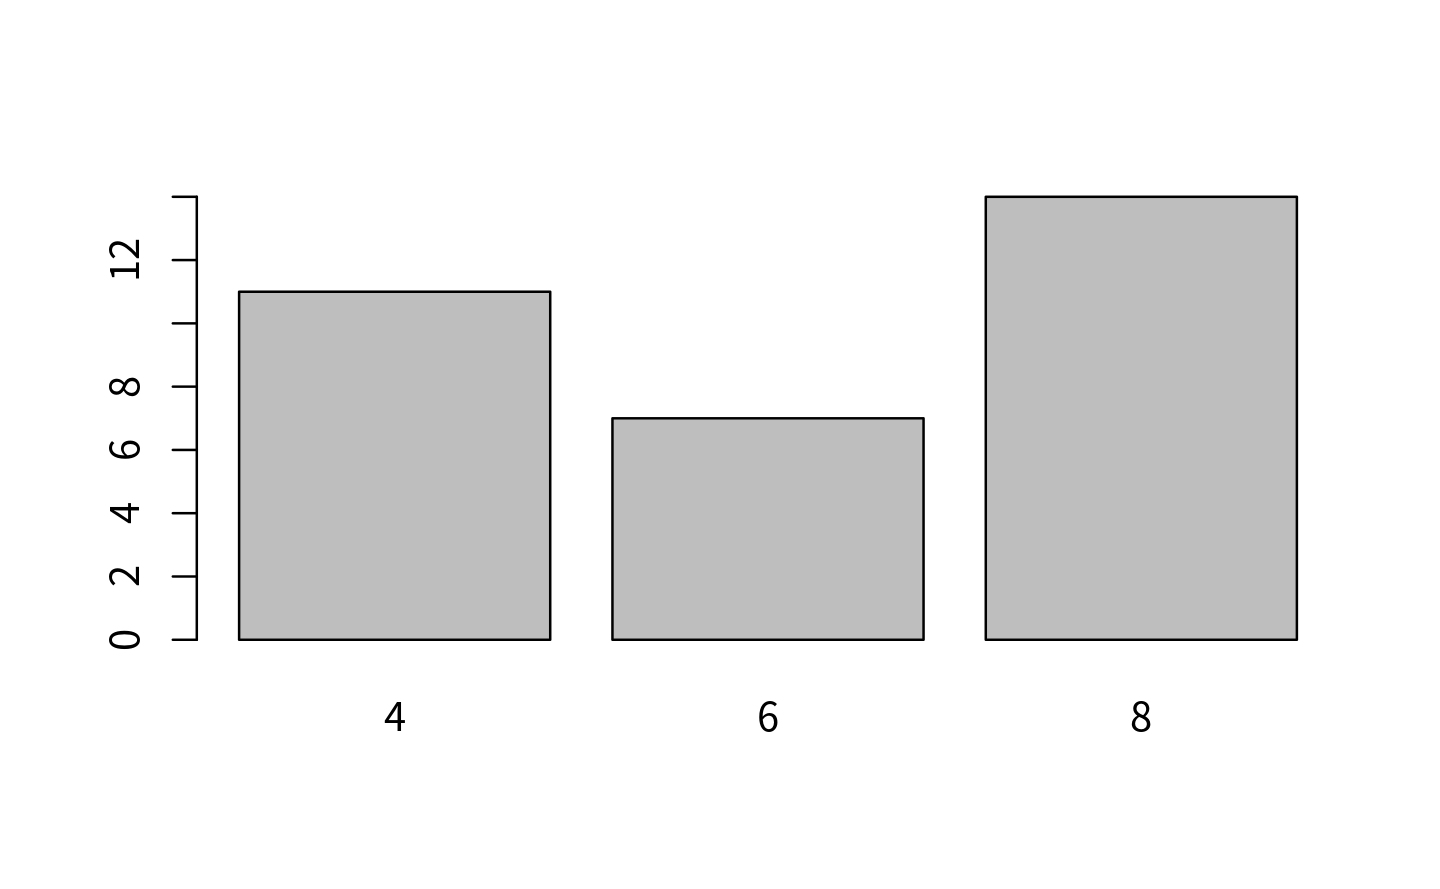
\includegraphics[width=0.7\linewidth]{rmi_copy_test_files/figure-latex/unnamed-chunk-10-1} \end{center}

::: sidebar

\begin{Shaded}
\begin{Highlighting}[]
\NormalTok{v<-}\KeywordTok{as.vector}\NormalTok{(}\KeywordTok{table}\NormalTok{(mtcars}\OperatorTok{$}\NormalTok{cyl))}
\KeywordTok{barplot}\NormalTok{(v)}
\NormalTok{m<-}\KeywordTok{as.matrix}\NormalTok{(}\KeywordTok{table}\NormalTok{(mtcars}\OperatorTok{$}\NormalTok{cyl))}
\KeywordTok{barplot}\NormalTok{(m)}

\KeywordTok{barplot}\NormalTok{(}\KeywordTok{c}\NormalTok{(}\DecValTok{11}\NormalTok{,}\DecValTok{7}\NormalTok{,}\DecValTok{4}\NormalTok{))}
\end{Highlighting}
\end{Shaded}

\begin{center}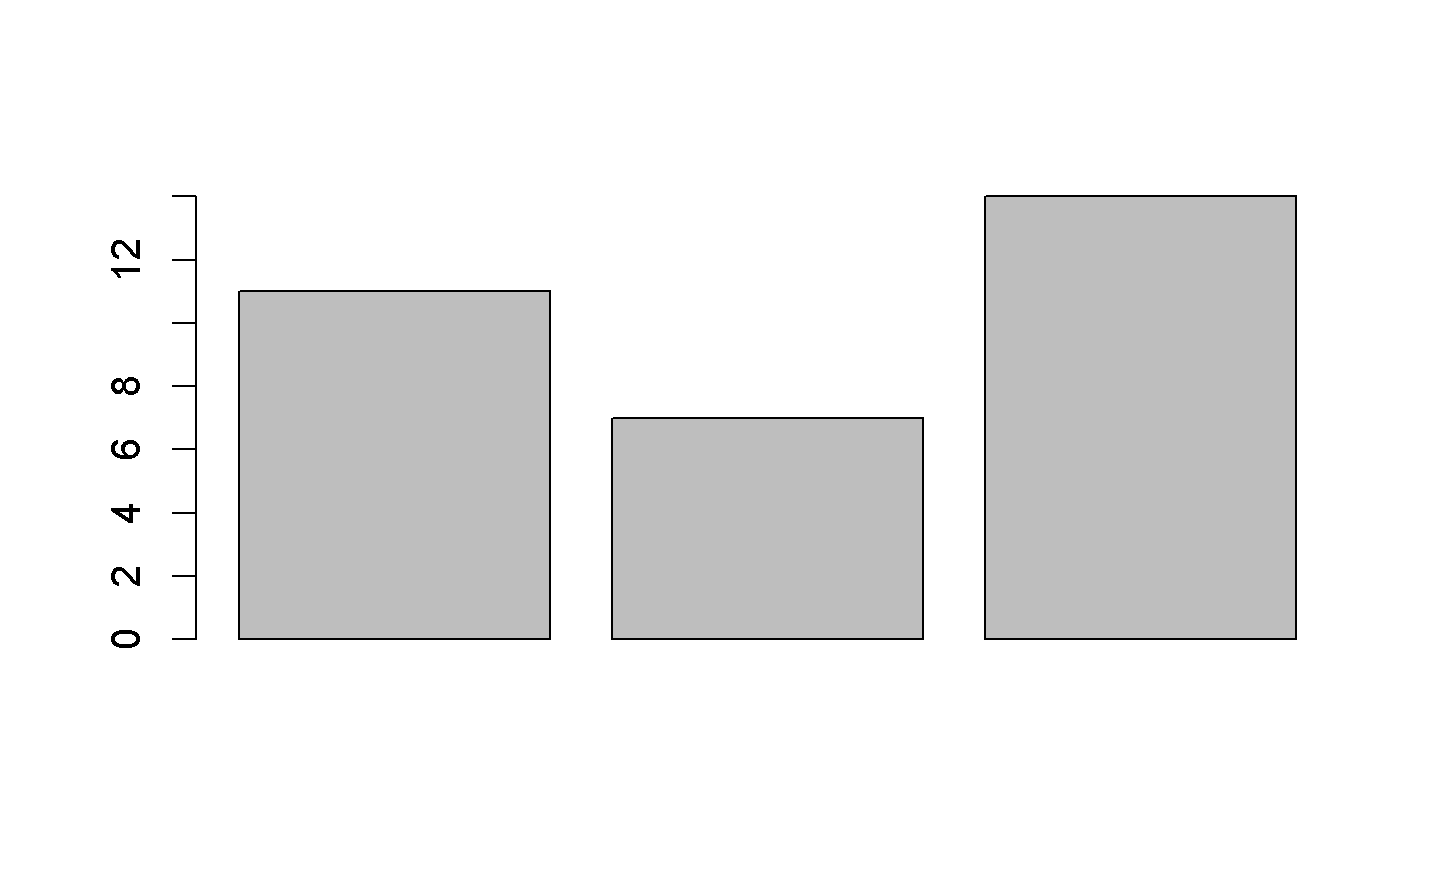
\includegraphics[width=0.7\linewidth]{rmi_copy_test_files/figure-latex/unnamed-chunk-11-1} 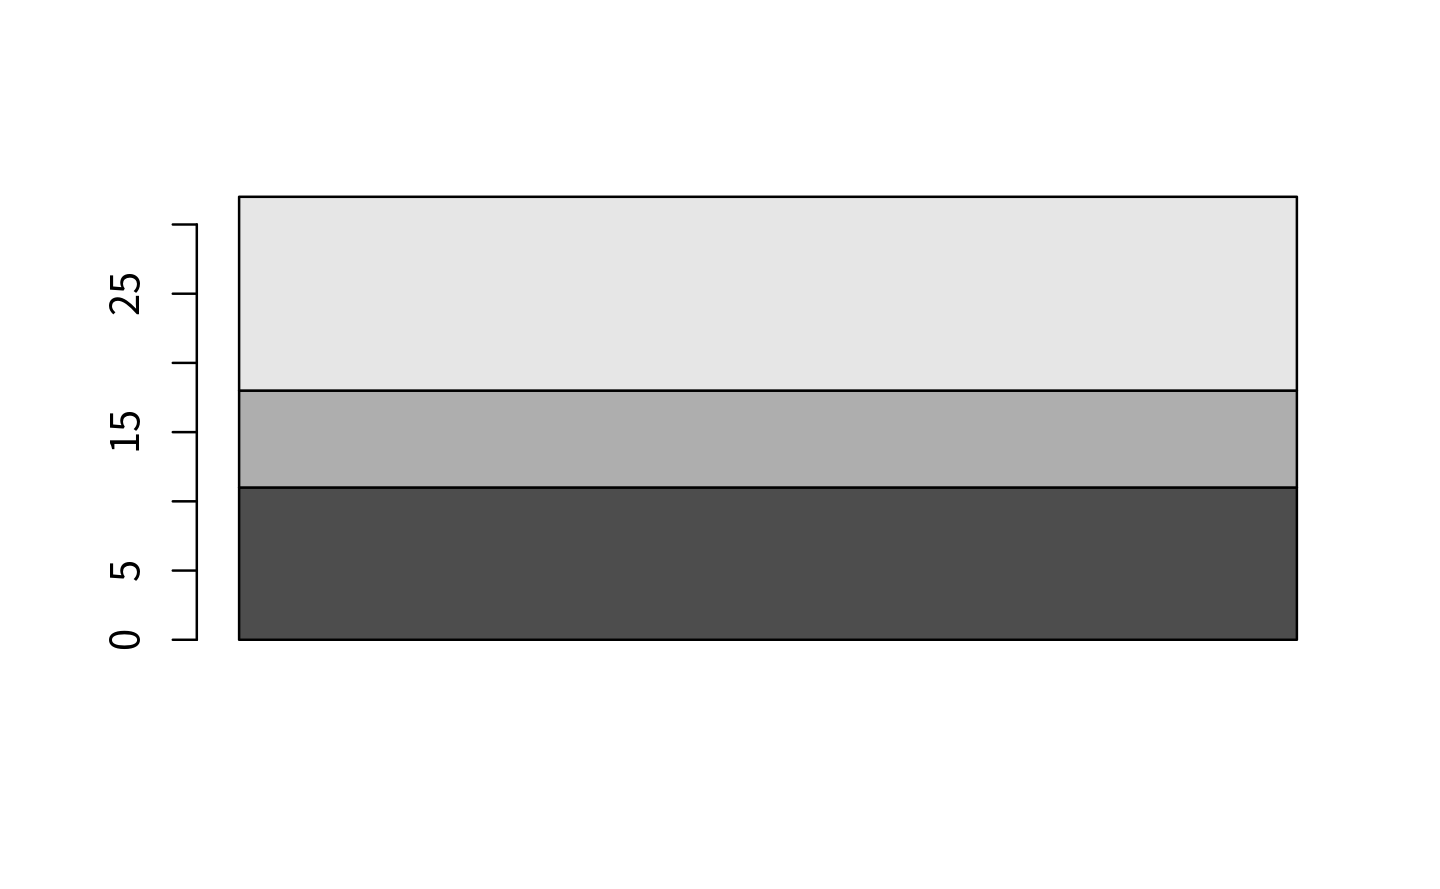
\includegraphics[width=0.7\linewidth]{rmi_copy_test_files/figure-latex/unnamed-chunk-11-2} 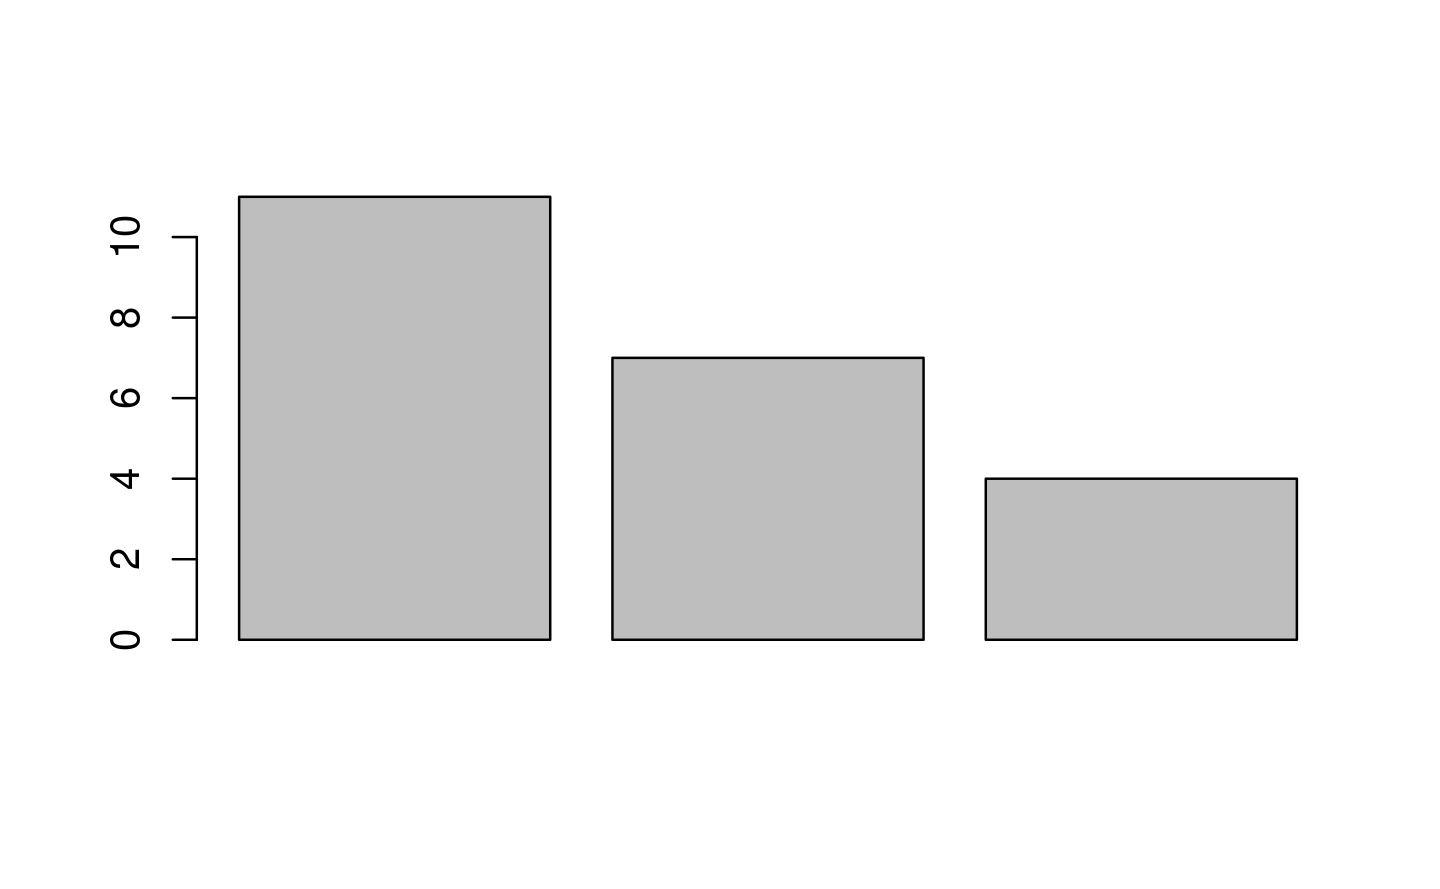
\includegraphics[width=0.7\linewidth]{rmi_copy_test_files/figure-latex/unnamed-chunk-11-3} \end{center}

:::

\begin{Shaded}
\begin{Highlighting}[]
\KeywordTok{barplot}\NormalTok{(mtcars}\OperatorTok{$}\NormalTok{mpg)}
\KeywordTok{barplot}\NormalTok{(mtcars}\OperatorTok{$}\NormalTok{cyl)}
\end{Highlighting}
\end{Shaded}

\begin{center}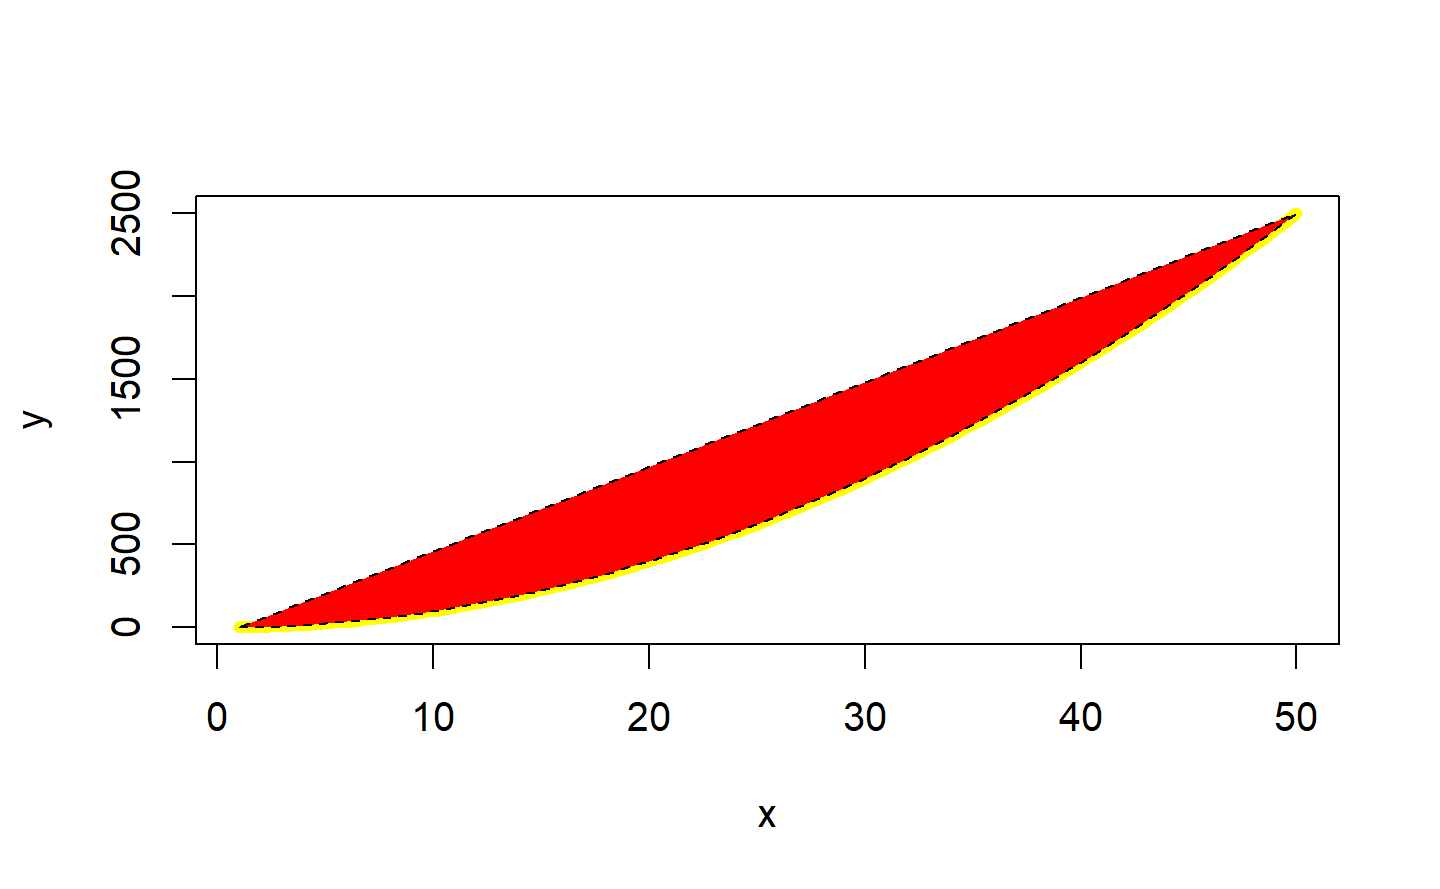
\includegraphics[width=0.7\linewidth]{rmi_copy_test_files/figure-latex/unnamed-chunk-12-1} 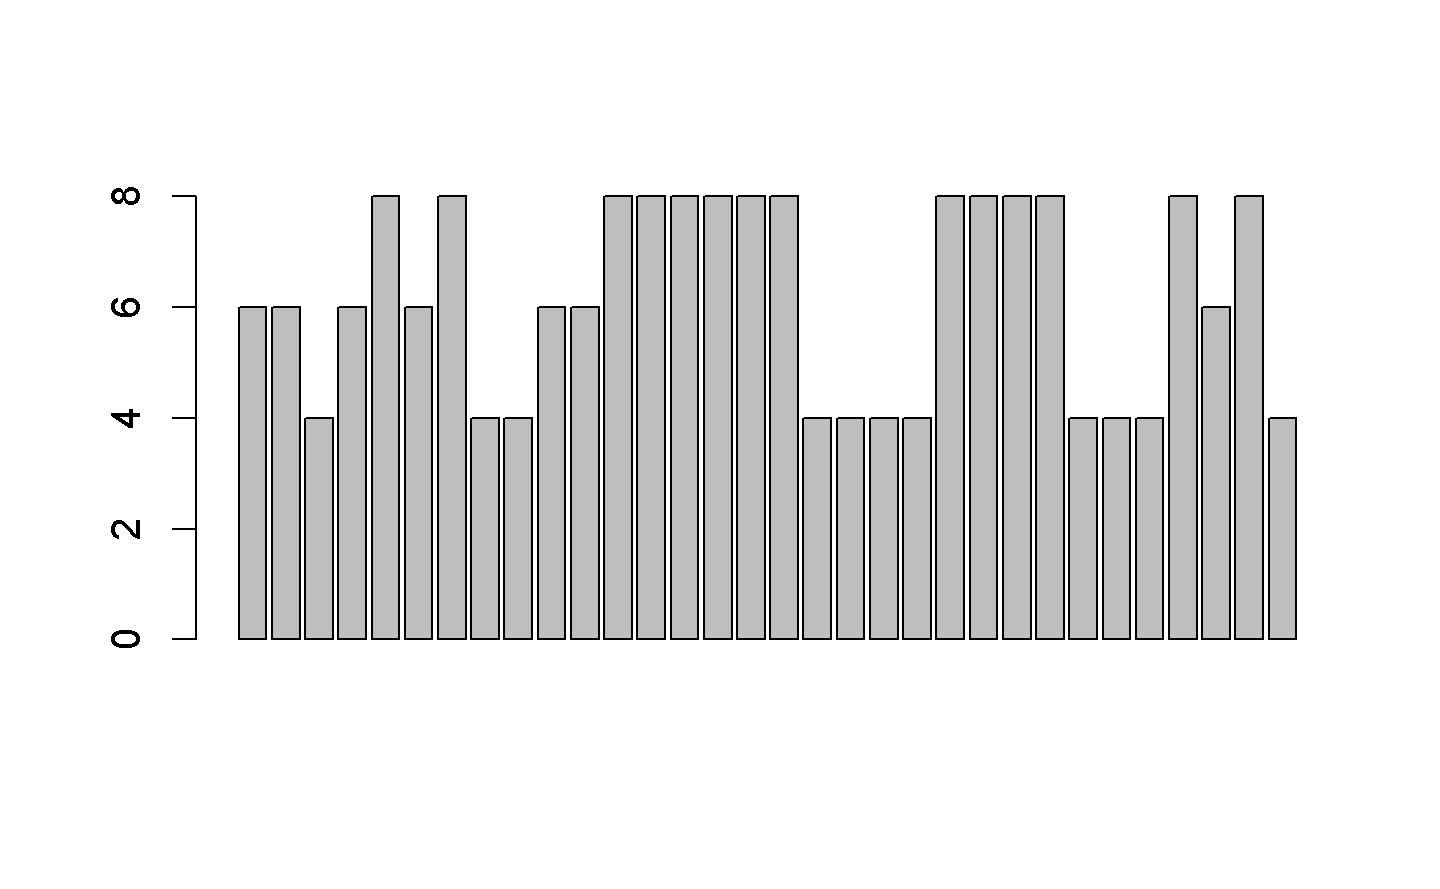
\includegraphics[width=0.7\linewidth]{rmi_copy_test_files/figure-latex/unnamed-chunk-12-2} \end{center}

\section{assignment}\label{assignment}

\textless{}-和 -\textgreater{} 是一對 ,可以向左和向右賦值\\
= 是單向的 ,作用和\textless{}-基本相同,但對函數中的變數通常使用=\\
\textless{}\textless{}- 這個是全域賦值
,跟變數的作用域有關,一般不會用到

\begin{Shaded}
\begin{Highlighting}[]
\NormalTok{##Delete x (if it exists)}
\KeywordTok{rm}\NormalTok{(x)}
\end{Highlighting}
\end{Shaded}

\begin{Shaded}
\begin{Highlighting}[]
\KeywordTok{mean}\NormalTok{(}\DataTypeTok{x =} \DecValTok{1}\OperatorTok{:}\DecValTok{10}\NormalTok{) }\CommentTok{#[1] 5.5}
\end{Highlighting}
\end{Shaded}

\begin{Shaded}
\begin{Highlighting}[]
\NormalTok{x }\CommentTok{#Error: object 'x' not found}
\end{Highlighting}
\end{Shaded}

Here x is declared within the function 's scope of the function, so it
doesn 't exist in the user workspace. Now, let 's run the same piece of
code with using the \textless{}- operator:

\begin{Shaded}
\begin{Highlighting}[]
\KeywordTok{mean}\NormalTok{(x <-}\StringTok{ }\DecValTok{1}\OperatorTok{:}\DecValTok{10}\NormalTok{) }\CommentTok{# [1] 5.5}
\end{Highlighting}
\end{Shaded}

\begin{Shaded}
\begin{Highlighting}[]
\NormalTok{x}
\end{Highlighting}
\end{Shaded}

\begin{quote}
x \# {[}1{]} 1 2 3 4 5 6 7 8 9 10
\end{quote}

This time the x variable is declared within the user workspace. When
does the assignment take place ? In the code above, you may be tempted
to thing that we ``assign 1:10 to x, then calculate the mean.'' This
would be true for \#languages such as C, but it isn 't true in R.
Consider the following function:

\begin{Shaded}
\begin{Highlighting}[]
\NormalTok{a <-}\StringTok{ }\DecValTok{1}
\NormalTok{f <-}\StringTok{ }\ControlFlowTok{function}\NormalTok{(a) }\KeywordTok{return}\NormalTok{(}\OtherTok{TRUE}\NormalTok{)}
\NormalTok{f <-}\StringTok{ }\KeywordTok{f}\NormalTok{(a <-}\StringTok{ }\NormalTok{a }\OperatorTok{+}\StringTok{ }\DecValTok{1}\NormalTok{);}
\CommentTok{# 輸出:TRUE}
\NormalTok{a }\CommentTok{# 結果=1 }
\end{Highlighting}
\end{Shaded}

Notice that the value of a hasn 't changed! In R, the value of a will
only change if we need to evaluate the argument in the function. This
can lead to unpredictable behaviour:

\begin{Shaded}
\begin{Highlighting}[]
\NormalTok{f <-}\StringTok{ }\ControlFlowTok{function}\NormalTok{(a) }\ControlFlowTok{if}\NormalTok{ (}\KeywordTok{runif}\NormalTok{(}\DecValTok{1}\NormalTok{) }\OperatorTok{>}\StringTok{ }\FloatTok{0.5}\NormalTok{) }\OtherTok{TRUE} \ControlFlowTok{else}\NormalTok{ a}
    \KeywordTok{f}\NormalTok{(a <-}\StringTok{ }\NormalTok{a }\OperatorTok{+}\StringTok{ }\DecValTok{1}\NormalTok{);}
\NormalTok{a }\CommentTok{# result 2}
\end{Highlighting}
\end{Shaded}

\begin{Shaded}
\begin{Highlighting}[]
\KeywordTok{f}\NormalTok{(a <-}\StringTok{ }\NormalTok{a }\OperatorTok{+}\StringTok{ }\DecValTok{1}\NormalTok{);}
\end{Highlighting}
\end{Shaded}

\begin{Shaded}
\begin{Highlighting}[]
\CommentTok{# TRUE}
\NormalTok{a }\CommentTok{# 2}
\end{Highlighting}
\end{Shaded}

\begin{Shaded}
\begin{Highlighting}[]
\KeywordTok{f}\NormalTok{(a <-}\StringTok{ }\NormalTok{a }\OperatorTok{+}\StringTok{ }\DecValTok{1}\NormalTok{);}
\end{Highlighting}
\end{Shaded}

\begin{Shaded}
\begin{Highlighting}[]
\NormalTok{a }\CommentTok{#3}
\end{Highlighting}
\end{Shaded}

=用在參數指派 例如

\begin{Shaded}
\begin{Highlighting}[]
\KeywordTok{matrix}\NormalTok{(}\DecValTok{1}\OperatorTok{:}\DecValTok{20}\NormalTok{, }\DataTypeTok{ncol =} \DecValTok{4}\NormalTok{)}
\end{Highlighting}
\end{Shaded}

如果

\begin{Shaded}
\begin{Highlighting}[]
\KeywordTok{matrix}\NormalTok{(}\DecValTok{1}\OperatorTok{:}\DecValTok{20}\NormalTok{, ncol <-}\StringTok{ }\DecValTok{4}\NormalTok{)}
\end{Highlighting}
\end{Shaded}

\begin{Shaded}
\begin{Highlighting}[]
\NormalTok{ncol}
\end{Highlighting}
\end{Shaded}

會產生一個變數 ncol 結論:x\textless{}-3
\textless{}-會在全局產生變數x然後指派3

\begin{Shaded}
\begin{Highlighting}[]
\NormalTok{(x <-}\StringTok{ }\DecValTok{3}\NormalTok{)}
\end{Highlighting}
\end{Shaded}

\begin{Shaded}
\begin{Highlighting}[]
\CommentTok{#rm(list = ls())}
\KeywordTok{rm}\NormalTok{(x)}
\KeywordTok{ls}\NormalTok{()}
\end{Highlighting}
\end{Shaded}

\begin{Shaded}
\begin{Highlighting}[]
\NormalTok{(}\DataTypeTok{x =} \DecValTok{3}\NormalTok{)}
\end{Highlighting}
\end{Shaded}

\begin{Shaded}
\begin{Highlighting}[]
\KeywordTok{ls}\NormalTok{()}
\end{Highlighting}
\end{Shaded}

因為x是參數名稱不是變數,看mean help

\chapter{data type}\label{data-type}

\section{基本操作}

\subsection{指派}

雖然也可以用=但是,R的設計是使用\textless{}-。

\begin{Shaded}
\begin{Highlighting}[]
\NormalTok{a <-}\StringTok{ }\DecValTok{3}
\end{Highlighting}
\end{Shaded}

\texttt{a\textless{}-3}是一個指派的敘述句,不會回饋資訊到螢幕上。如果要知道a的內容是甚麼,就打入\texttt{a}
或者\texttt{(a\textless{}-3)}

\begin{Shaded}
\begin{Highlighting}[]
\NormalTok{    a}
\end{Highlighting}
\end{Shaded}

\begin{Shaded}
\begin{Highlighting}[]
\NormalTok{(a<-}\DecValTok{3}\NormalTok{)}
\end{Highlighting}
\end{Shaded}

\begin{Shaded}
\begin{Highlighting}[]
\NormalTok{b <-}\StringTok{ }\KeywordTok{sqrt}\NormalTok{(a }\OperatorTok{*}\StringTok{ }\NormalTok{a }\OperatorTok{+}\StringTok{ }\DecValTok{5}\NormalTok{)}
\NormalTok{b}
\end{Highlighting}
\end{Shaded}

在session中的如果要列出已經定義過的變數,可以利用ls

\begin{Shaded}
\begin{Highlighting}[]
\KeywordTok{ls}\NormalTok{()}
\end{Highlighting}
\end{Shaded}

\subsection{資源}

\begin{itemize}
\tightlist
\item
  \href{http://adv-r.had.co.nz/Data-structures.html}{資料結構}
\end{itemize}

\section{介紹}

在R語言中,型態不須經過宣告(declared)。
一個變數的型態經由assignment的過程決定,即\textless{}-右邊的R-Objects。也就是在指派變數值的時候,同時決定了型態。基本的
R-object有 −

\begin{itemize}
\tightlist
\item
  Vectors\\
\item
  Lists\\
\item
  Matrices
\item
  Arrays
\item
  Factors
\item
  Data Frames
\end{itemize}

最簡單的是vector物件,atomic vector 有6種data types(有時也叫做 6
個classes)

\begin{longtable}[]{@{}ll@{}}
\toprule
Data Type & Example\tabularnewline
\midrule
\endhead
Logical & TRUE, FALSE\tabularnewline
Numeric & 1.3, 5, 99\tabularnewline
Integer & 3L, 24L, 0L\tabularnewline
Complex & 5 + 4i\tabularnewline
Character & `b' , ``good'', ``TRUE'', `23.4'\tabularnewline
Raw & ``Hello'' is stored as 48 65 6c 6c 6f\tabularnewline
\bottomrule
\end{longtable}

\begin{Shaded}
\begin{Highlighting}[]
\NormalTok{v <-}\StringTok{ }\OtherTok{TRUE} 
\KeywordTok{print}\NormalTok{(}\KeywordTok{class}\NormalTok{(v))}
\end{Highlighting}
\end{Shaded}

\begin{Shaded}
\begin{Highlighting}[]
\NormalTok{v <-}\StringTok{ }\FloatTok{23.5}
\KeywordTok{print}\NormalTok{(}\KeywordTok{class}\NormalTok{(v))}
\end{Highlighting}
\end{Shaded}

\begin{Shaded}
\begin{Highlighting}[]
\NormalTok{v <-}\StringTok{ }\NormalTok{2L}
\KeywordTok{print}\NormalTok{(}\KeywordTok{class}\NormalTok{(v))}
\end{Highlighting}
\end{Shaded}

\begin{Shaded}
\begin{Highlighting}[]
\NormalTok{v <-}\StringTok{ }\DecValTok{2}\OperatorTok{+}\NormalTok{5i}
\KeywordTok{print}\NormalTok{(}\KeywordTok{class}\NormalTok{(v))}
\end{Highlighting}
\end{Shaded}

\begin{Shaded}
\begin{Highlighting}[]
\NormalTok{v <-}\StringTok{ "TRUE"}
\KeywordTok{print}\NormalTok{(}\KeywordTok{class}\NormalTok{(v))}
\end{Highlighting}
\end{Shaded}

\begin{Shaded}
\begin{Highlighting}[]
\NormalTok{v <-}\StringTok{ }\KeywordTok{charToRaw}\NormalTok{(}\StringTok{"Hello"}\NormalTok{)}
\KeywordTok{print}\NormalTok{(}\KeywordTok{class}\NormalTok{(v))}
\end{Highlighting}
\end{Shaded}

\section{實數的比較}

\begin{Shaded}
\begin{Highlighting}[]
\NormalTok{x <-}\StringTok{ }\KeywordTok{seq}\NormalTok{(}\DecValTok{0}\NormalTok{, }\DecValTok{1}\NormalTok{, }\DataTypeTok{by =} \FloatTok{0.2}\NormalTok{)}
\NormalTok{y <-}\StringTok{ }\KeywordTok{seq}\NormalTok{(}\DecValTok{0}\NormalTok{, }\DecValTok{1}\NormalTok{, }\DataTypeTok{by =} \FloatTok{0.2}\NormalTok{)}
\NormalTok{y[}\DecValTok{4}\NormalTok{]}
\end{Highlighting}
\end{Shaded}

\begin{Shaded}
\begin{Highlighting}[]
\NormalTok{x[}\DecValTok{3}\NormalTok{]}
\end{Highlighting}
\end{Shaded}

\begin{Shaded}
\begin{Highlighting}[]
\DecValTok{1} \OperatorTok{-}\StringTok{ }\NormalTok{x[}\DecValTok{3}\NormalTok{]}
\end{Highlighting}
\end{Shaded}

\begin{Shaded}
\begin{Highlighting}[]
\NormalTok{y[}\DecValTok{4}\NormalTok{] }\OperatorTok{==}\StringTok{ }\DecValTok{1} \OperatorTok{-}\StringTok{ }\NormalTok{x[}\DecValTok{3}\NormalTok{]}
\end{Highlighting}
\end{Shaded}

\begin{Shaded}
\begin{Highlighting}[]
\NormalTok{y[}\DecValTok{4}\NormalTok{] }\OperatorTok{>}\StringTok{ }\DecValTok{1} \OperatorTok{-}\StringTok{ }\NormalTok{x[}\DecValTok{3}\NormalTok{]}
\end{Highlighting}
\end{Shaded}

\begin{Shaded}
\begin{Highlighting}[]
\NormalTok{## note:}
\KeywordTok{all.equal}\NormalTok{(y[}\DecValTok{4}\NormalTok{], }\DecValTok{1} \OperatorTok{-}\StringTok{ }\NormalTok{x[}\DecValTok{3}\NormalTok{])}
\end{Highlighting}
\end{Shaded}

\begin{Shaded}
\begin{Highlighting}[]
\NormalTok{## Q: what is the result of : 1-0.4 ==0.6}
\end{Highlighting}
\end{Shaded}

\begin{Shaded}
\begin{Highlighting}[]
\FloatTok{0.1}\OperatorTok{+}\FloatTok{0.2} \OperatorTok{==}\StringTok{ }\FloatTok{0.3}
\end{Highlighting}
\end{Shaded}

\begin{Shaded}
\begin{Highlighting}[]
\KeywordTok{all.equal}\NormalTok{(}\FloatTok{0.1}\OperatorTok{+}\FloatTok{0.2}\NormalTok{,}\FloatTok{0.3}\NormalTok{)}
\end{Highlighting}
\end{Shaded}

\section{字串}

\href{https://www.gastonsanchez.com/r4strings/chars.html}{參考}

\subsection{建立字串}

可以是 雙引號中``'' 或 單引號中''。
字串中如果有雙引號,或單引號,則如下表示:\\
``\,`這個'來自'那個'\,''

\begin{Shaded}
\begin{Highlighting}[]
\NormalTok{a <-}\StringTok{ "hello"}
\NormalTok{a}
\end{Highlighting}
\end{Shaded}

\begin{Shaded}
\begin{Highlighting}[]
\KeywordTok{typeof}\NormalTok{(a)}
\end{Highlighting}
\end{Shaded}

利用函數:character()
這個函數的參數,為整數,建立一個list,裡面的元素都是空字串

\begin{Shaded}
\begin{Highlighting}[]
\CommentTok{# 變數ex初始化為character vector,參看後面的討論}
\NormalTok{(ex <-}\StringTok{ }\KeywordTok{character}\NormalTok{(}\DecValTok{0}\NormalTok{))}
\end{Highlighting}
\end{Shaded}

\begin{Shaded}
\begin{Highlighting}[]
\KeywordTok{length}\NormalTok{(ex)}
\end{Highlighting}
\end{Shaded}

\begin{Shaded}
\begin{Highlighting}[]
\KeywordTok{class}\NormalTok{(ex)}
\end{Highlighting}
\end{Shaded}

\begin{Shaded}
\begin{Highlighting}[]
\CommentTok{# 如果剛剛沒有設定ex <- character(0),這裡會發生錯誤}
\NormalTok{(ex[}\DecValTok{1}\NormalTok{] <-}\StringTok{ "first"}\NormalTok{)}
\end{Highlighting}
\end{Shaded}

\begin{Shaded}
\begin{Highlighting}[]
\CommentTok{# check its length again}
\KeywordTok{length}\NormalTok{(ex)}
\end{Highlighting}
\end{Shaded}

索引可以用跳的:

\begin{Shaded}
\begin{Highlighting}[]
\NormalTok{(ex[}\DecValTok{4}\NormalTok{] <-}\StringTok{ "fourth"}\NormalTok{)}
\end{Highlighting}
\end{Shaded}

\begin{Shaded}
\begin{Highlighting}[]
\KeywordTok{length}\NormalTok{(ex)}
\end{Highlighting}
\end{Shaded}

\begin{Shaded}
\begin{Highlighting}[]
\KeywordTok{typeof}\NormalTok{(ex)}
\end{Highlighting}
\end{Shaded}

\begin{Shaded}
\begin{Highlighting}[]
\NormalTok{ex}
\end{Highlighting}
\end{Shaded}

跳過的索引,內容自動為\texttt{NA}.

\subsection{空字串}

引號內連空白都沒有的字串:
(比較上面利用character(5)可以建立5個元素為空字串的vector。)

\begin{Shaded}
\begin{Highlighting}[]
\CommentTok{# empty string}
\NormalTok{empty_str <-}\StringTok{ ""}
\NormalTok{empty_str}
\end{Highlighting}
\end{Shaded}

\begin{Shaded}
\begin{Highlighting}[]
\CommentTok{# class}
\KeywordTok{class}\NormalTok{(empty_str)}
\end{Highlighting}
\end{Shaded}

\subsubsection{討論character(0)}\label{character0}

前面說character(2),可以傳回長度2,每個元素都是空白字串``''的向量,那麼character(0)是甚麼?
除了前面提到的變數初始化為向量(也許可以說是向量宣告) 例如,整數也是這樣

\begin{Shaded}
\begin{Highlighting}[]
\NormalTok{zz<-}\KeywordTok{integer}\NormalTok{(}\DecValTok{0}\NormalTok{)}
\NormalTok{zz[}\DecValTok{4}\NormalTok{]=}\DecValTok{6}
\NormalTok{zz}
\end{Highlighting}
\end{Shaded}

這裡對character(0)做一些測試:

\begin{Shaded}
\begin{Highlighting}[]
\NormalTok{ex1<-}\KeywordTok{character}\NormalTok{(}\DecValTok{0}\NormalTok{) }
\NormalTok{ex2<-}\StringTok{""}

\KeywordTok{typeof}\NormalTok{(ex1)}
\end{Highlighting}
\end{Shaded}

\begin{Shaded}
\begin{Highlighting}[]
\KeywordTok{typeof}\NormalTok{(ex2)}
\end{Highlighting}
\end{Shaded}

\begin{Shaded}
\begin{Highlighting}[]
\KeywordTok{str}\NormalTok{(ex1)}
\end{Highlighting}
\end{Shaded}

\begin{Shaded}
\begin{Highlighting}[]
\KeywordTok{str}\NormalTok{(ex2)}
\end{Highlighting}
\end{Shaded}

\begin{Shaded}
\begin{Highlighting}[]
\KeywordTok{class}\NormalTok{(ex1)}
\end{Highlighting}
\end{Shaded}

\begin{Shaded}
\begin{Highlighting}[]
\KeywordTok{class}\NormalTok{(ex2)}
\end{Highlighting}
\end{Shaded}

\begin{Shaded}
\begin{Highlighting}[]
\KeywordTok{is.list}\NormalTok{(ex1)}
\end{Highlighting}
\end{Shaded}

\begin{Shaded}
\begin{Highlighting}[]
\KeywordTok{is.list}\NormalTok{(ex2)}
\end{Highlighting}
\end{Shaded}

surprise: 一個字元也是向量。

\begin{Shaded}
\begin{Highlighting}[]
\KeywordTok{is.vector}\NormalTok{(ex1)}
\end{Highlighting}
\end{Shaded}

\begin{Shaded}
\begin{Highlighting}[]
\KeywordTok{is.vector}\NormalTok{(ex2)}
\end{Highlighting}
\end{Shaded}

\begin{Shaded}
\begin{Highlighting}[]
\KeywordTok{length}\NormalTok{(ex1)}
\end{Highlighting}
\end{Shaded}

\begin{Shaded}
\begin{Highlighting}[]
\KeywordTok{length}\NormalTok{(ex2)}
\end{Highlighting}
\end{Shaded}

最後,這兩個是不是相等

\begin{Shaded}
\begin{Highlighting}[]
\NormalTok{ex1}\OperatorTok{==}\NormalTok{ex2}
\end{Highlighting}
\end{Shaded}

\section{型態操作is family}\label{is-family}

is.numeric(), is.integer(), and is.double() \#\# 型態轉換 as family

\begin{Shaded}
\begin{Highlighting}[]
\NormalTok{a<-}\KeywordTok{c}\NormalTok{(}\OtherTok{TRUE}\NormalTok{,}\OtherTok{FALSE}\NormalTok{)}
\KeywordTok{as.numeric}\NormalTok{(a)}
\end{Highlighting}
\end{Shaded}

\begin{Shaded}
\begin{Highlighting}[]
\NormalTok{an<-}\KeywordTok{as.logical}\NormalTok{(a)}
\NormalTok{an}
\end{Highlighting}
\end{Shaded}

\section{vector}\label{vector}

利用\texttt{c}函數,可以使用vector存放一個以上的數字。

\begin{Shaded}
\begin{Highlighting}[]
\NormalTok{a =}\StringTok{ }\KeywordTok{c}\NormalTok{(}\DecValTok{1}\NormalTok{, }\DecValTok{2}\NormalTok{, }\DecValTok{3}\NormalTok{, }\DecValTok{4}\NormalTok{, }\DecValTok{5}\NormalTok{)}
\NormalTok{a1 =}\StringTok{ }\DecValTok{1}\OperatorTok{:}\DecValTok{5}
\end{Highlighting}
\end{Shaded}

有關list的運算:加減乘除等等

\begin{Shaded}
\begin{Highlighting}[]
\NormalTok{a =}\StringTok{ }\KeywordTok{c}\NormalTok{(}\DecValTok{1}\NormalTok{, }\DecValTok{2}\NormalTok{, }\DecValTok{3}\NormalTok{, }\DecValTok{4}\NormalTok{, }\DecValTok{5}\NormalTok{)}
\NormalTok{a}\OperatorTok{+}\DecValTok{1}
\end{Highlighting}
\end{Shaded}

\begin{Shaded}
\begin{Highlighting}[]
\KeywordTok{mean}\NormalTok{(a)}
\end{Highlighting}
\end{Shaded}

\begin{Shaded}
\begin{Highlighting}[]
\KeywordTok{var}\NormalTok{(a)}
\end{Highlighting}
\end{Shaded}

\begin{Shaded}
\begin{Highlighting}[]
\KeywordTok{summary}\NormalTok{(a)}
\end{Highlighting}
\end{Shaded}

list的元素,利用中括號

\begin{Shaded}
\begin{Highlighting}[]
\NormalTok{a =}\StringTok{ }\DecValTok{2}\OperatorTok{:}\DecValTok{6}
\NormalTok{a[}\DecValTok{1}\NormalTok{]}
\end{Highlighting}
\end{Shaded}

\begin{Shaded}
\begin{Highlighting}[]
\NormalTok{a[}\DecValTok{2}\NormalTok{]}
\end{Highlighting}
\end{Shaded}

\begin{Shaded}
\begin{Highlighting}[]
\NormalTok{a[}\DecValTok{0}\NormalTok{]}
\end{Highlighting}
\end{Shaded}

\begin{Shaded}
\begin{Highlighting}[]
\NormalTok{a[}\DecValTok{6}\NormalTok{]}
\end{Highlighting}
\end{Shaded}

在R中,的最小的索引值為1base.如果給索引為0,可以知道資料是否被排序。
超出索引範圍得到``NA。

\begin{Shaded}
\begin{Highlighting}[]
\NormalTok{a=}\DecValTok{2}\OperatorTok{:}\DecValTok{6}
\NormalTok{x =}\StringTok{ }\NormalTok{a[}\DecValTok{6}\NormalTok{]}
\end{Highlighting}
\end{Shaded}

::: sidebar 如何判斷是否NA

\begin{Shaded}
\begin{Highlighting}[]
\NormalTok{x }\OperatorTok{==}\StringTok{ }\OtherTok{NA}
\end{Highlighting}
\end{Shaded}

上面的比較沒有意義,和NA的任何運算都是NA

\begin{Shaded}
\begin{Highlighting}[]
\NormalTok{r =}\StringTok{ }\NormalTok{x }\OperatorTok{==}\StringTok{ }\OtherTok{NA}
\NormalTok{r}
\end{Highlighting}
\end{Shaded}

結論:任何變數和NA運算,結果還是NA\\
另一種方法

\begin{Shaded}
\begin{Highlighting}[]
\KeywordTok{print}\NormalTok{(x }\OperatorTok{==}\StringTok{ }\OtherTok{NA}\NormalTok{)}
\end{Highlighting}
\end{Shaded}

如何判斷NA ? \texttt{is.na()}

\begin{Shaded}
\begin{Highlighting}[]
    \KeywordTok{is.na}\NormalTok{(a[}\DecValTok{6}\NormalTok{])}
\end{Highlighting}
\end{Shaded}

:::

初始化向量,可以利用a\textless{}-10 或指定numeric(double)型態

\begin{Shaded}
\begin{Highlighting}[]
\NormalTok{a <-}\StringTok{ }\KeywordTok{numeric}\NormalTok{(}\DecValTok{10}\NormalTok{) }
\NormalTok{a}
\end{Highlighting}
\end{Shaded}

如果想要知到變數的資料型別,利用函數typeof()

typeof()函數回傳的結果是``字串''

\begin{Shaded}
\begin{Highlighting}[]
\KeywordTok{typeof}\NormalTok{(a) }\CommentTok{# 結果是"double"}
\end{Highlighting}
\end{Shaded}

\begin{Shaded}
\begin{Highlighting}[]
\NormalTok{s =}\StringTok{ }\KeywordTok{typeof}\NormalTok{(a)}
\NormalTok{s}
\end{Highlighting}
\end{Shaded}

\begin{Shaded}
\begin{Highlighting}[]
\KeywordTok{typeof}\NormalTok{(s) }\CommentTok{#結果是 "character"}
\end{Highlighting}
\end{Shaded}

\subsection{練習範例}

Q1. a,a1,a2 屬於甚麼型態

\begin{Shaded}
\begin{Highlighting}[]
\NormalTok{a =}\StringTok{ }\DecValTok{1}\OperatorTok{:}\DecValTok{4}
\NormalTok{a1 =}\StringTok{ }\KeywordTok{c}\NormalTok{(}\DecValTok{1}\NormalTok{, }\DecValTok{2}\NormalTok{, }\DecValTok{3}\NormalTok{, }\DecValTok{4}\NormalTok{)}
\NormalTok{a2 =}\StringTok{ }\KeywordTok{numeric}\NormalTok{(}\DecValTok{4}\NormalTok{)}
\end{Highlighting}
\end{Shaded}

A1

Q2:a3的長度是甚麼?2,或6

\begin{Shaded}
\begin{Highlighting}[]
\NormalTok{a1<-}\KeywordTok{c}\NormalTok{(}\DecValTok{1}\NormalTok{,}\DecValTok{2}\NormalTok{,}\DecValTok{3}\NormalTok{)}
\NormalTok{a2<-}\KeywordTok{c}\NormalTok{(}\DecValTok{2}\NormalTok{,}\DecValTok{3}\NormalTok{,}\DecValTok{4}\NormalTok{)}
\NormalTok{a3<-}\KeywordTok{c}\NormalTok{(a1,a2)}
\end{Highlighting}
\end{Shaded}

HINT: a1 a2 a3;length(a3)

::: sidebar \#\# 字串和vector 在EXCEL中,vector
一般指的是只放元素為數字的陣列(array);而陣列是可以存數字和文字的區域。table是有欄位的陣列。
但是在R語言中,vector 只是元素型態相同即可。 :::

\begin{Shaded}
\begin{Highlighting}[]
\NormalTok{a <-}\StringTok{ "hello"}
\NormalTok{a}
\end{Highlighting}
\end{Shaded}

\begin{Shaded}
\begin{Highlighting}[]
\KeywordTok{typeof}\NormalTok{(a)}
\end{Highlighting}
\end{Shaded}

\begin{Shaded}
\begin{Highlighting}[]
\NormalTok{b <-}\StringTok{ }\KeywordTok{c}\NormalTok{(}\StringTok{"hello"}\NormalTok{, }\StringTok{"there"}\NormalTok{)}
\NormalTok{b}
\end{Highlighting}
\end{Shaded}

\begin{Shaded}
\begin{Highlighting}[]
\NormalTok{b[}\DecValTok{1}\NormalTok{]}
\end{Highlighting}
\end{Shaded}

\begin{Shaded}
\begin{Highlighting}[]
\KeywordTok{typeof}\NormalTok{(b)}
\end{Highlighting}
\end{Shaded}

\begin{Shaded}
\begin{Highlighting}[]
\NormalTok{(}\DataTypeTok{a =} \KeywordTok{character}\NormalTok{(}\DecValTok{5}\NormalTok{)) }\CommentTok{# 產生5個空白字串}
\end{Highlighting}
\end{Shaded}

\begin{Shaded}
\begin{Highlighting}[]
\NormalTok{(}\DataTypeTok{b =}\NormalTok{ letters[}\DecValTok{1}\OperatorTok{:}\DecValTok{4}\NormalTok{]) }\CommentTok{# 注意,letters不是函數}
\end{Highlighting}
\end{Shaded}

\begin{Shaded}
\begin{Highlighting}[]
\NormalTok{letters}
\end{Highlighting}
\end{Shaded}

因為c函數的運算結果為vector,因此下例中,其元素都是字串

\begin{Shaded}
\begin{Highlighting}[]
\NormalTok{ (a<-}\KeywordTok{c}\NormalTok{(}\StringTok{"d"}\NormalTok{,}\DecValTok{4}\NormalTok{,}\OtherTok{TRUE}\NormalTok{))}
\end{Highlighting}
\end{Shaded}

問題: 怎樣知道r是空集合?

\begin{Shaded}
\begin{Highlighting}[]
\NormalTok{y <-}\StringTok{ }\NormalTok{letters[}\DecValTok{1}\OperatorTok{:}\DecValTok{3}\NormalTok{] }
\NormalTok{z <-}\StringTok{ }\NormalTok{letters[}\DecValTok{4}\OperatorTok{:}\DecValTok{6}\NormalTok{] }
\NormalTok{r<-}\KeywordTok{intersect}\NormalTok{(y,z) }
\NormalTok{r}
\end{Highlighting}
\end{Shaded}

\begin{Shaded}
\begin{Highlighting}[]
\KeywordTok{is.na}\NormalTok{(r)}
\end{Highlighting}
\end{Shaded}

另外,當vector有多個字串,而使用索引0的時候,也會出現
\texttt{character(0)},例如:

\begin{Shaded}
\begin{Highlighting}[]
\NormalTok{string <-}\StringTok{ }\KeywordTok{c}\NormalTok{(}\StringTok{'sun'}\NormalTok{, }\StringTok{'sky'}\NormalTok{, }\StringTok{'clouds'}\NormalTok{)}
\NormalTok{string[}\DecValTok{0}\NormalTok{]}
\end{Highlighting}
\end{Shaded}

\subsection{vector 相關的運算}\label{vector-}

連續數字可以利用操作元\texttt{:},例如:

x \textless{}- 1:7; x y \textless{}- 2:-2; y

比較複雜的序列可以利用函數 seq() ,例如

\begin{Shaded}
\begin{Highlighting}[]
\KeywordTok{seq}\NormalTok{(}\DecValTok{1}\NormalTok{, }\DecValTok{3}\NormalTok{, }\DataTypeTok{by=}\FloatTok{0.2}\NormalTok{)          }\CommentTok{# specify step size}
\end{Highlighting}
\end{Shaded}

\begin{Shaded}
\begin{Highlighting}[]
 \KeywordTok{seq}\NormalTok{(}\DecValTok{1}\NormalTok{, }\DecValTok{5}\NormalTok{, }\DataTypeTok{length.out=}\DecValTok{4}\NormalTok{)    }\CommentTok{# specify length of the vector}
\end{Highlighting}
\end{Shaded}

\subsection{如何存取vector中的元素}\label{vector}

元素索引可以利用 logical, integer or character vector.

如果利用整數索引,則從1開始.但是,如果索引值給的是負數(例如-2),則除了2號元素以外,都會被傳回。但是不能同時有正負。同時,浮點數會被truncated。

\begin{Shaded}
\begin{Highlighting}[]
\OperatorTok{>}\StringTok{ }\NormalTok{x}
\NormalTok{[}\DecValTok{1}\NormalTok{]  }\DecValTok{0}  \DecValTok{2}  \DecValTok{4}  \DecValTok{6}  \DecValTok{8} \DecValTok{10}
\OperatorTok{>}\StringTok{ }\NormalTok{x[}\DecValTok{3}\NormalTok{]           }\CommentTok{# access 3rd element}
\NormalTok{[}\DecValTok{1}\NormalTok{] }\DecValTok{4}
\OperatorTok{>}\StringTok{ }\NormalTok{x[}\KeywordTok{c}\NormalTok{(}\DecValTok{2}\NormalTok{, }\DecValTok{4}\NormalTok{)]     }\CommentTok{# access 2nd and 4th element}
\NormalTok{[}\DecValTok{1}\NormalTok{] }\DecValTok{2} \DecValTok{6}
\OperatorTok{>}\StringTok{ }\NormalTok{x[}\OperatorTok{-}\DecValTok{1}\NormalTok{]          }\CommentTok{# access all but 1st element}
\NormalTok{[}\DecValTok{1}\NormalTok{]  }\DecValTok{2}  \DecValTok{4}  \DecValTok{6}  \DecValTok{8} \DecValTok{10}
\OperatorTok{>}\StringTok{ }\NormalTok{x[}\KeywordTok{c}\NormalTok{(}\DecValTok{2}\NormalTok{, }\OperatorTok{-}\DecValTok{4}\NormalTok{)]    }\CommentTok{# 不能混合正負}
\NormalTok{Error }\ControlFlowTok{in}\NormalTok{ x[}\KeywordTok{c}\NormalTok{(}\DecValTok{2}\NormalTok{, }\OperatorTok{-}\DecValTok{4}\NormalTok{)] }\OperatorTok{:}\StringTok{ }\NormalTok{only }\DecValTok{0}\StringTok{'s may be mixed with negative subscripts}
\StringTok{> x[c(2.4, 3.54)]    # real numbers are truncated to integers}
\StringTok{[1] 2 4}
\end{Highlighting}
\end{Shaded}

\subsection{邏輯做為索引}

說是索引有點誤導,可以認為是元素篩選。例如

\begin{Shaded}
\begin{Highlighting}[]
\OperatorTok{>}\StringTok{ }\NormalTok{x[}\KeywordTok{c}\NormalTok{(}\OtherTok{TRUE}\NormalTok{, }\OtherTok{FALSE}\NormalTok{, }\OtherTok{FALSE}\NormalTok{, }\OtherTok{TRUE}\NormalTok{)]}
\NormalTok{[}\DecValTok{1}\NormalTok{] }\OperatorTok{-}\DecValTok{3}  \DecValTok{3}
\OperatorTok{>}\StringTok{ }\NormalTok{x[x }\OperatorTok{<}\StringTok{ }\DecValTok{0}\NormalTok{]  }\CommentTok{# filtering vectors based on conditions}
\NormalTok{[}\DecValTok{1}\NormalTok{] }\OperatorTok{-}\DecValTok{3} \OperatorTok{-}\DecValTok{1}
\OperatorTok{>}\StringTok{ }\NormalTok{x[x }\OperatorTok{>}\StringTok{ }\DecValTok{0}\NormalTok{]}
\NormalTok{[}\DecValTok{1}\NormalTok{] }\DecValTok{3}
\end{Highlighting}
\end{Shaded}

In the above example, the expression x\textgreater{}0 will yield a
logical vector (FALSE, FALSE, FALSE, TRUE) which is then used for
indexing.

\subsection{利用字串( character vector)
作為索引}\label{-character-vector-}

每個元素可以有名稱:

\begin{Shaded}
\begin{Highlighting}[]
\OperatorTok{>}\StringTok{ }\NormalTok{x <-}\StringTok{ }\KeywordTok{c}\NormalTok{(}\StringTok{"first"}\NormalTok{=}\DecValTok{3}\NormalTok{, }\StringTok{"second"}\NormalTok{=}\DecValTok{0}\NormalTok{, }\StringTok{"third"}\NormalTok{=}\DecValTok{9}\NormalTok{)}
\OperatorTok{>}\StringTok{ }\KeywordTok{names}\NormalTok{(x)}
\NormalTok{[}\DecValTok{1}\NormalTok{] }\StringTok{"first"}  \StringTok{"second"} \StringTok{"third"} 
\OperatorTok{>}\StringTok{ }\NormalTok{x[}\StringTok{"second"}\NormalTok{]}
\NormalTok{second }
\DecValTok{0} 
\OperatorTok{>}\StringTok{ }\NormalTok{x[}\KeywordTok{c}\NormalTok{(}\StringTok{"first"}\NormalTok{, }\StringTok{"third"}\NormalTok{)]}
\NormalTok{first third }
\DecValTok{3}     \DecValTok{9}
\end{Highlighting}
\end{Shaded}

\begin{Shaded}
\begin{Highlighting}[]
\NormalTok{a<-}\KeywordTok{c}\NormalTok{(}\DataTypeTok{x=}\DecValTok{1}\OperatorTok{:}\DecValTok{2}\NormalTok{,}\DataTypeTok{y=}\DecValTok{3}\OperatorTok{:}\DecValTok{4}\NormalTok{)}
\NormalTok{a[}\StringTok{"x1"}\NormalTok{] }\CommentTok{# 不是a[x1]}
\end{Highlighting}
\end{Shaded}

\protect\hyperlink{section-1}{}
和{[}\protect\hyperlink{section-1}{}{]}的差別:\\
原來是甚麼(例如,list
或vector),\protect\hyperlink{section-1}{}只是返回子集合(仍然是list或vector),但是{[}\protect\hyperlink{section-1}{}{]}則是返回內容.

\begin{Shaded}
\begin{Highlighting}[]
\NormalTok{x <-}\StringTok{ }\KeywordTok{c}\NormalTok{(}\DataTypeTok{a =} \DecValTok{1}\NormalTok{, }\DataTypeTok{b =} \DecValTok{2}\NormalTok{, }\DataTypeTok{c =} \DecValTok{3}\NormalTok{)}
\NormalTok{x[}\StringTok{"a"}\NormalTok{]}
\end{Highlighting}
\end{Shaded}

\begin{Shaded}
\begin{Highlighting}[]
\NormalTok{x[[}\StringTok{"a"}\NormalTok{]]}
\end{Highlighting}
\end{Shaded}

\begin{Shaded}
\begin{Highlighting}[]
\NormalTok{x[}\DecValTok{1}\NormalTok{]}
\end{Highlighting}
\end{Shaded}

\begin{Shaded}
\begin{Highlighting}[]
\NormalTok{x[[}\DecValTok{1}\NormalTok{]]}
\end{Highlighting}
\end{Shaded}

和list的區別是 1. \$ 1. 不必有``''

\begin{Shaded}
\begin{Highlighting}[]
\NormalTok{a1<-}\KeywordTok{list}\NormalTok{(}\DataTypeTok{x=}\DecValTok{1}\OperatorTok{:}\DecValTok{2}\NormalTok{,}\DataTypeTok{y=}\DecValTok{3}\OperatorTok{:}\DecValTok{4}\NormalTok{)}
\NormalTok{a1}\OperatorTok{$}\NormalTok{x}
\end{Highlighting}
\end{Shaded}

\subsection{How to modify a vector in
R?}\label{how-to-modify-a-vector-in-r}

We can modify a vector using the assignment operator.

We can use the techniques discussed above to access specific elements
and modify them.

If we want to truncate the elements, we can use reassignments.

\begin{Shaded}
\begin{Highlighting}[]
\OperatorTok{>}\StringTok{ }\NormalTok{x}
\NormalTok{[}\DecValTok{1}\NormalTok{] }\OperatorTok{-}\DecValTok{3} \OperatorTok{-}\DecValTok{2} \OperatorTok{-}\DecValTok{1}  \DecValTok{0}  \DecValTok{1}  \DecValTok{2}
\OperatorTok{>}\StringTok{ }\NormalTok{x[}\DecValTok{2}\NormalTok{] <-}\StringTok{ }\DecValTok{0}\NormalTok{; x        }\CommentTok{# modify 2nd element}
\NormalTok{[}\DecValTok{1}\NormalTok{] }\OperatorTok{-}\DecValTok{3}  \DecValTok{0} \OperatorTok{-}\DecValTok{1}  \DecValTok{0}  \DecValTok{1}  \DecValTok{2}
\OperatorTok{>}\StringTok{ }\NormalTok{x[x}\OperatorTok{<}\DecValTok{0}\NormalTok{] <-}\StringTok{ }\DecValTok{5}\NormalTok{; x   }\CommentTok{# modify elements less than 0}
\NormalTok{[}\DecValTok{1}\NormalTok{] }\DecValTok{5} \DecValTok{0} \DecValTok{5} \DecValTok{0} \DecValTok{1} \DecValTok{2}
\OperatorTok{>}\StringTok{ }\NormalTok{x <-}\StringTok{ }\NormalTok{x[}\DecValTok{1}\OperatorTok{:}\DecValTok{4}\NormalTok{]; x      }\CommentTok{# truncate x to first 4 elements}
\NormalTok{[}\DecValTok{1}\NormalTok{] }\DecValTok{5} \DecValTok{0} \DecValTok{5} \DecValTok{0}
\end{Highlighting}
\end{Shaded}

\subsection{How to delete a Vector?}\label{how-to-delete-a-vector}

We can delete a vector by simply assigning a NULL to it.

\begin{Shaded}
\begin{Highlighting}[]
\OperatorTok{>}\StringTok{ }\NormalTok{x}
\NormalTok{[}\DecValTok{1}\NormalTok{] }\OperatorTok{-}\DecValTok{3} \OperatorTok{-}\DecValTok{2} \OperatorTok{-}\DecValTok{1}  \DecValTok{0}  \DecValTok{1}  \DecValTok{2}
\OperatorTok{>}\StringTok{ }\NormalTok{x <-}\StringTok{ }\OtherTok{NULL}
\OperatorTok{>}\StringTok{ }\NormalTok{x}
\OtherTok{NULL}
\OperatorTok{>}\StringTok{ }\NormalTok{x[}\DecValTok{4}\NormalTok{]}
\OtherTok{NULL}
\end{Highlighting}
\end{Shaded}

\section{List}\label{list}

Lists 是一個R物件。其元素內容可以是不同型態,例如 numbers, strings,
vectors,matrix 或者是另一個 list,甚至是函數。。

\subsection{建立 List}\label{-list}

函數\texttt{list()} 可以建立list.

包含多種type的List: strings, numbers, vectors and a logical values.

\begin{Shaded}
\begin{Highlighting}[]
\NormalTok{list_data <-}\StringTok{ }\KeywordTok{list}\NormalTok{(}\StringTok{"Red"}\NormalTok{, }\StringTok{"Green"}\NormalTok{, }\KeywordTok{c}\NormalTok{(}\DecValTok{21}\NormalTok{,}\DecValTok{32}\NormalTok{,}\DecValTok{11}\NormalTok{), }\OtherTok{TRUE}\NormalTok{, }\FloatTok{51.23}\NormalTok{, }\FloatTok{119.1}\NormalTok{)}
\KeywordTok{print}\NormalTok{(list_data)}
\end{Highlighting}
\end{Shaded}

  \#\#\# Naming List Elements

The list elements can be given names and they can be accessed using
these names.

\begin{Shaded}
\begin{Highlighting}[]
\CommentTok{#Create a list containing a vector, a matrix and a list.}
\NormalTok{list_data <-}\StringTok{ }\KeywordTok{list}\NormalTok{(}\KeywordTok{c}\NormalTok{(}\StringTok{"Jan"}\NormalTok{,}\StringTok{"Feb"}\NormalTok{,}\StringTok{"Mar"}\NormalTok{), }\KeywordTok{matrix}\NormalTok{(}\KeywordTok{c}\NormalTok{(}\DecValTok{3}\NormalTok{,}\DecValTok{9}\NormalTok{,}\DecValTok{5}\NormalTok{,}\DecValTok{1}\NormalTok{,}\OperatorTok{-}\DecValTok{2}\NormalTok{,}\DecValTok{8}\NormalTok{), }\DataTypeTok{nrow =} \DecValTok{2}\NormalTok{),}
   \KeywordTok{list}\NormalTok{(}\StringTok{"green"}\NormalTok{,}\FloatTok{12.3}\NormalTok{))}

\CommentTok{#Give names to the elements in the list.}
\KeywordTok{names}\NormalTok{(list_data) <-}\StringTok{ }\KeywordTok{c}\NormalTok{(}\StringTok{"1st Quarter"}\NormalTok{, }\StringTok{"A_Matrix"}\NormalTok{, }\StringTok{"A Inner list"}\NormalTok{)}

\CommentTok{#Show the list.}
\KeywordTok{print}\NormalTok{(list_data)}
\end{Highlighting}
\end{Shaded}

::: sidebar
這裡討論一下為甚麼在R語言堅持\texttt{\textless{}-}而不是\texttt{=}的一個原因

將列名的vector和list ,白話文意思就是將每個元素命名。

\begin{Shaded}
\begin{Highlighting}[]
\NormalTok{x=}\KeywordTok{c}\NormalTok{(}\DecValTok{1}\NormalTok{,}\DecValTok{2}\NormalTok{,}\DecValTok{3}\NormalTok{)}
\KeywordTok{names}\NormalTok{(x)<-}\KeywordTok{c}\NormalTok{(}\StringTok{'a'}\NormalTok{,}\StringTok{'b'}\NormalTok{,}\StringTok{'c'}\NormalTok{)}
\NormalTok{x}
\end{Highlighting}
\end{Shaded}

一般的程式語言,不會用到這種文法,例如,在其他程式語言中,直覺上應該是有一個\texttt{names()},然後用法如下:

\begin{Shaded}
\begin{Highlighting}[]
\NormalTok{names(x,c(}\CharTok{'a'}\NormalTok{,}\CharTok{'b'}\NormalTok{,}\CharTok{'c'}\NormalTok{) )}
\end{Highlighting}
\end{Shaded}

但如果是matrix,被命名的就是欄位?答案是:\textbf{NO}。而是紀錄名稱?答案也是\textbf{NO}.而是給每個元素命名。

\begin{Shaded}
\begin{Highlighting}[]
\NormalTok{x<-}\KeywordTok{matrix}\NormalTok{(}\KeywordTok{runif}\NormalTok{(}\DecValTok{9}\NormalTok{),}\DataTypeTok{nrow=}\DecValTok{3}\NormalTok{)}
\KeywordTok{names}\NormalTok{(x)<-}\KeywordTok{c}\NormalTok{(}\StringTok{'a'}\NormalTok{,}\StringTok{'b'}\NormalTok{,}\StringTok{'c'}\NormalTok{)}
\NormalTok{x}
\end{Highlighting}
\end{Shaded}

\begin{Shaded}
\begin{Highlighting}[]
\KeywordTok{rownames}\NormalTok{(x)<-}\KeywordTok{c}\NormalTok{(}\StringTok{'x'}\NormalTok{,}\StringTok{'y'}\NormalTok{,}\StringTok{'z'}\NormalTok{)}
\KeywordTok{print}\NormalTok{(x,}\DataTypeTok{row.names=}\NormalTok{T)}
\end{Highlighting}
\end{Shaded}

問:在上面的例子中x是一個矩陣,x{[}``a''{]}會傳回甚麼? :::
但是在data.frame的結構中,names()\textless{}- 給定的是欄位名稱

\begin{Shaded}
\begin{Highlighting}[]
\NormalTok{xd<-}\KeywordTok{data.frame}\NormalTok{(x)}
\KeywordTok{names}\NormalTok{(xd)<-}\KeywordTok{c}\NormalTok{(}\StringTok{'a'}\NormalTok{,}\StringTok{'b'}\NormalTok{,}\StringTok{'c'}\NormalTok{)}
\NormalTok{xd}
\end{Highlighting}
\end{Shaded}

\subsection{存取 List 元素}\label{-list-}

\begin{Shaded}
\begin{Highlighting}[]
\CommentTok{# 3個元素,分別是list, matrix, list}
\NormalTok{list_data <-}\StringTok{ }\KeywordTok{list}\NormalTok{(}\KeywordTok{c}\NormalTok{(}\StringTok{"Jan"}\NormalTok{,}\StringTok{"Feb"}\NormalTok{,}\StringTok{"Mar"}\NormalTok{), }\KeywordTok{matrix}\NormalTok{(}\KeywordTok{c}\NormalTok{(}\DecValTok{3}\NormalTok{,}\DecValTok{9}\NormalTok{,}\DecValTok{5}\NormalTok{,}\DecValTok{1}\NormalTok{,}\OperatorTok{-}\DecValTok{2}\NormalTok{,}\DecValTok{8}\NormalTok{), }\DataTypeTok{nrow =} \DecValTok{2}\NormalTok{),}
   \KeywordTok{list}\NormalTok{(}\StringTok{"green"}\NormalTok{,}\FloatTok{12.3}\NormalTok{))}

\CommentTok{# 給名稱}
\KeywordTok{names}\NormalTok{(list_data) <-}\StringTok{ }\KeywordTok{c}\NormalTok{(}\StringTok{"1st Quarter"}\NormalTok{, }\StringTok{"A_Matrix"}\NormalTok{, }\StringTok{"A Inner list"}\NormalTok{)}

\CommentTok{# Access the first element of the list.}
\KeywordTok{print}\NormalTok{(list_data[}\DecValTok{1}\NormalTok{])}
\end{Highlighting}
\end{Shaded}

\begin{Shaded}
\begin{Highlighting}[]
\CommentTok{# Access the thrid element. As it is also a list, all its elements will be printed.}
\KeywordTok{print}\NormalTok{(list_data[}\DecValTok{3}\NormalTok{])}
\end{Highlighting}
\end{Shaded}

\begin{Shaded}
\begin{Highlighting}[]
\CommentTok{# Access the list element using the name of the element.}
\KeywordTok{print}\NormalTok{(list_data}\OperatorTok{$}\NormalTok{A_Matrix)}
\end{Highlighting}
\end{Shaded}

\subsection{Manipulating List
Elements}\label{manipulating-list-elements}

We can add, delete and update list elements as shown below. We can add
and delete elements only at the end of a list. But we can update any
element.

\begin{Shaded}
\begin{Highlighting}[]
\CommentTok{# Create a list containing a vector, a matrix and a list.}
\NormalTok{list_data <-}\StringTok{ }\KeywordTok{list}\NormalTok{(}\KeywordTok{c}\NormalTok{(}\StringTok{"Jan"}\NormalTok{,}\StringTok{"Feb"}\NormalTok{,}\StringTok{"Mar"}\NormalTok{), }\KeywordTok{matrix}\NormalTok{(}\KeywordTok{c}\NormalTok{(}\DecValTok{3}\NormalTok{,}\DecValTok{9}\NormalTok{,}\DecValTok{5}\NormalTok{,}\DecValTok{1}\NormalTok{,}\OperatorTok{-}\DecValTok{2}\NormalTok{,}\DecValTok{8}\NormalTok{), }\DataTypeTok{nrow =} \DecValTok{2}\NormalTok{),}
   \KeywordTok{list}\NormalTok{(}\StringTok{"green"}\NormalTok{,}\FloatTok{12.3}\NormalTok{))}

\CommentTok{# Give names to the elements in the list.}
\KeywordTok{names}\NormalTok{(list_data) <-}\StringTok{ }\KeywordTok{c}\NormalTok{(}\StringTok{"1st Quarter"}\NormalTok{, }\StringTok{"A_Matrix"}\NormalTok{, }\StringTok{"A Inner list"}\NormalTok{)}

\CommentTok{# Add element at the end of the list.}
\NormalTok{list_data[}\DecValTok{4}\NormalTok{] <-}\StringTok{ "New element"}
\KeywordTok{print}\NormalTok{(list_data[}\DecValTok{4}\NormalTok{])}
\end{Highlighting}
\end{Shaded}

\begin{Shaded}
\begin{Highlighting}[]
\CommentTok{# Remove the last element.}
\NormalTok{list_data[}\DecValTok{4}\NormalTok{] <-}\StringTok{ }\OtherTok{NULL}

\CommentTok{# Print the 4th Element.}
\KeywordTok{print}\NormalTok{(list_data[}\DecValTok{4}\NormalTok{])}
\end{Highlighting}
\end{Shaded}

\begin{Shaded}
\begin{Highlighting}[]
\CommentTok{# Update the 3rd Element.}
\NormalTok{list_data[}\DecValTok{3}\NormalTok{] <-}\StringTok{ "updated element"}
\KeywordTok{print}\NormalTok{(list_data[}\DecValTok{3}\NormalTok{])}
\end{Highlighting}
\end{Shaded}

\subsection{Merging Lists}\label{merging-lists}

You can merge many lists into one list by placing all the lists inside
one list() function.

\begin{Shaded}
\begin{Highlighting}[]
\CommentTok{# Create two lists.}
\NormalTok{list1 <-}\StringTok{ }\KeywordTok{list}\NormalTok{(}\DecValTok{1}\NormalTok{,}\DecValTok{2}\NormalTok{,}\DecValTok{3}\NormalTok{)}
\NormalTok{list2 <-}\StringTok{ }\KeywordTok{list}\NormalTok{(}\StringTok{"Sun"}\NormalTok{,}\StringTok{"Mon"}\NormalTok{,}\StringTok{"Tue"}\NormalTok{)}

\CommentTok{# Merge the two lists.}
\NormalTok{merged.list <-}\StringTok{ }\KeywordTok{c}\NormalTok{(list1,list2)}

\CommentTok{# Print the merged list.}
\KeywordTok{print}\NormalTok{(merged.list)}
\end{Highlighting}
\end{Shaded}

我們說函數\texttt{c()}是一個處理向量的函數,但是這裡的list裡面有多個型態,所以為甚麼用\texttt{c()}?
因為,對\texttt{c()}而言,兩個元素都是list
。而在R語言中,向量的意思,只要元素同型態就行。

\subsection{List 轉 Vector}\label{list--vector}

函數 \texttt{unlist()}

\begin{Shaded}
\begin{Highlighting}[]
\CommentTok{# Create lists.}
\NormalTok{list1 <-}\StringTok{ }\KeywordTok{list}\NormalTok{(}\DecValTok{1}\OperatorTok{:}\DecValTok{5}\NormalTok{)}
\KeywordTok{print}\NormalTok{(list1)}
\end{Highlighting}
\end{Shaded}

\begin{Shaded}
\begin{Highlighting}[]
\NormalTok{list2 <-}\KeywordTok{list}\NormalTok{(}\DecValTok{10}\OperatorTok{:}\DecValTok{14}\NormalTok{)}
\KeywordTok{print}\NormalTok{(list2)}
\end{Highlighting}
\end{Shaded}

\begin{Shaded}
\begin{Highlighting}[]
\CommentTok{# Convert the lists to vectors.}
\NormalTok{v1 <-}\StringTok{ }\KeywordTok{unlist}\NormalTok{(list1)}
\NormalTok{v2 <-}\StringTok{ }\KeywordTok{unlist}\NormalTok{(list2)}

\KeywordTok{print}\NormalTok{(v1)}
\end{Highlighting}
\end{Shaded}

\begin{Shaded}
\begin{Highlighting}[]
\KeywordTok{print}\NormalTok{(v2)}
\end{Highlighting}
\end{Shaded}

\begin{Shaded}
\begin{Highlighting}[]
\CommentTok{# Now add the vectors}
\NormalTok{result <-}\StringTok{ }\NormalTok{v1}\OperatorTok{+}\NormalTok{v2}
\KeywordTok{print}\NormalTok{(result)}
\end{Highlighting}
\end{Shaded}

\subsection{比較vector, list中,字串的問題}\label{vector-list}

\begin{enumerate}
\def\labelenumi{\arabic{enumi}.}
\tightlist
\item
  Q length()函數可以知道vector,list
  的長度,但是為甚麼length(``hello'')的長度是1?
\end{enumerate}

\begin{Shaded}
\begin{Highlighting}[]
\NormalTok{a<-}\KeywordTok{c}\NormalTok{(}\StringTok{"hello"}\NormalTok{,}\StringTok{"r"}\NormalTok{)}
\KeywordTok{length}\NormalTok{(a)}
\end{Highlighting}
\end{Shaded}

\begin{Shaded}
\begin{Highlighting}[]
\KeywordTok{length}\NormalTok{(a[}\DecValTok{1}\NormalTok{])}
\end{Highlighting}
\end{Shaded}

\begin{Shaded}
\begin{Highlighting}[]
\KeywordTok{length}\NormalTok{(a[[}\DecValTok{1}\NormalTok{]])}
\end{Highlighting}
\end{Shaded}

\begin{Shaded}
\begin{Highlighting}[]
\KeywordTok{nchar}\NormalTok{(a[}\DecValTok{1}\NormalTok{])}
\end{Highlighting}
\end{Shaded}

\begin{Shaded}
\begin{Highlighting}[]
\KeywordTok{length}\NormalTok{(}\StringTok{"hello"}\NormalTok{)}
\end{Highlighting}
\end{Shaded}

\begin{enumerate}
\def\labelenumi{\arabic{enumi}.}
\tightlist
\item
  Q
\end{enumerate}

\begin{Shaded}
\begin{Highlighting}[]
\NormalTok{a<-}\KeywordTok{list}\NormalTok{(}\StringTok{"hello"}\NormalTok{,}\StringTok{"r"}\NormalTok{)}
\KeywordTok{length}\NormalTok{(a)}
\end{Highlighting}
\end{Shaded}

\begin{Shaded}
\begin{Highlighting}[]
\KeywordTok{length}\NormalTok{(a[}\DecValTok{1}\NormalTok{])}
\end{Highlighting}
\end{Shaded}

\begin{Shaded}
\begin{Highlighting}[]
\KeywordTok{length}\NormalTok{(a[[}\DecValTok{1}\NormalTok{]])}
\end{Highlighting}
\end{Shaded}

上面兩個答案的問題,和R怎樣建立字串有關 我猜是 ``hello'' 的記憶體結構是
list(ptr) ,ptr-\textgreater{}``hello''
也就是說紀錄在list中,當我問說length(``hello'')的時候,list的長度都是1。\\
總之,字串長度函數\texttt{nchar()}。

\section{data set build in}\label{data-set-build-in}

\subsection{List of pre-loaded data}\label{list-of-pre-loaded-data}

\begin{Shaded}
\begin{Highlighting}[]
\KeywordTok{data}\NormalTok{()}
\end{Highlighting}
\end{Shaded}

Loading a built-in R data

\begin{Shaded}
\begin{Highlighting}[]
\KeywordTok{data}\NormalTok{(mtcars) }
\end{Highlighting}
\end{Shaded}

\begin{Shaded}
\begin{Highlighting}[]
\KeywordTok{nrow}\NormalTok{(mtcars)}
\end{Highlighting}
\end{Shaded}

\begin{Shaded}
\begin{Highlighting}[]
\KeywordTok{ncol}\NormalTok{(mtcars)}
\end{Highlighting}
\end{Shaded}

\section{vector 函數範例}\label{vector-}

\subsection{cbind,rbind}\label{cbindrbind}

\begin{Shaded}
\begin{Highlighting}[]
\NormalTok{x<-}\KeywordTok{runif}\NormalTok{(}\DecValTok{5}\NormalTok{)}
\NormalTok{y<-}\KeywordTok{runif}\NormalTok{(}\DecValTok{6}\NormalTok{)}
\KeywordTok{cbind}\NormalTok{(x,y)}
\end{Highlighting}
\end{Shaded}

\subsection{函數diff}\label{diff}

Arguments\\
* x: a numeric vector or matrix containing the values to be
differenced.\\
* lag: an integer indicating which lag to use.\\
* differences: an integer indicating the order of the difference.\\
例如 diff(x,lag=d,differences=n) x{[}(1+d):n{]} - x{[}1:(n-d){]}

\section{matrix}\label{matrix}

矩陣的建立有多種方式,其中一種是利用向量轉填矩陣,填入的方式預設是以coumn為主要方向。

\begin{Shaded}
\begin{Highlighting}[]
\KeywordTok{matrix}\NormalTok{(}\KeywordTok{c}\NormalTok{(}\DecValTok{1}\NormalTok{,}\DecValTok{2}\NormalTok{,}\DecValTok{3}\NormalTok{,}\DecValTok{4}\NormalTok{,}\DecValTok{5}\NormalTok{,}\DecValTok{6}\NormalTok{),}\DecValTok{2}\NormalTok{,}\DecValTok{3}\NormalTok{)}
\end{Highlighting}
\end{Shaded}

問題: 怎樣產生\\
1 2 3\\
4 5 6\\
的矩陣

\begin{Shaded}
\begin{Highlighting}[]
\KeywordTok{diag}\NormalTok{(}\DecValTok{1}\NormalTok{, }\DataTypeTok{nrow =} \DecValTok{5}\NormalTok{)}
\end{Highlighting}
\end{Shaded}

\begin{Shaded}
\begin{Highlighting}[]
\KeywordTok{matrix}\NormalTok{(}\KeywordTok{c}\NormalTok{(}\DecValTok{1}\NormalTok{, }\DecValTok{2}\NormalTok{, }\DecValTok{3}\NormalTok{, }\DecValTok{4}\NormalTok{, }\DecValTok{5}\NormalTok{, }\DecValTok{6}\NormalTok{, }\DecValTok{7}\NormalTok{, }\DecValTok{8}\NormalTok{, }\DecValTok{9}\NormalTok{), }\DataTypeTok{nrow =} \DecValTok{3}\NormalTok{, }\DataTypeTok{byrow =} \OtherTok{TRUE}\NormalTok{, }\DataTypeTok{dimnames =} \KeywordTok{list}\NormalTok{(}\KeywordTok{c}\NormalTok{(}\StringTok{"r1"}\NormalTok{, }\StringTok{"r2"}\NormalTok{, }\StringTok{"r3"}\NormalTok{), }\KeywordTok{c}\NormalTok{(}\StringTok{"c1"}\NormalTok{, }\StringTok{"c2"}\NormalTok{, }\StringTok{"c3"}\NormalTok{)))}
\end{Highlighting}
\end{Shaded}

\begin{Shaded}
\begin{Highlighting}[]
\NormalTok{m1 <-}\StringTok{ }\KeywordTok{matrix}\NormalTok{(}\KeywordTok{c}\NormalTok{(}\DecValTok{1}\NormalTok{, }\DecValTok{2}\NormalTok{, }\DecValTok{3}\NormalTok{, }\DecValTok{4}\NormalTok{, }\DecValTok{5}\NormalTok{, }\DecValTok{6}\NormalTok{, }\DecValTok{7}\NormalTok{, }\DecValTok{8}\NormalTok{, }\DecValTok{9}\NormalTok{), }\DataTypeTok{ncol =} \DecValTok{3}\NormalTok{)}
\KeywordTok{rownames}\NormalTok{(m1) <-}\StringTok{ }\KeywordTok{c}\NormalTok{(}\StringTok{"r1"}\NormalTok{, }\StringTok{"r2"}\NormalTok{, }\StringTok{"r3"}\NormalTok{)}
\KeywordTok{colnames}\NormalTok{(m1) <-}\StringTok{ }\KeywordTok{c}\NormalTok{(}\StringTok{"c1"}\NormalTok{, }\StringTok{"c2"}\NormalTok{, }\StringTok{"c3"}\NormalTok{)}

\NormalTok{m1}
\end{Highlighting}
\end{Shaded}

\begin{Shaded}
\begin{Highlighting}[]
\NormalTok{ B =}\StringTok{ }\KeywordTok{matrix}\NormalTok{( }
    \KeywordTok{c}\NormalTok{(}\DecValTok{2}\NormalTok{, }\DecValTok{4}\NormalTok{, }\DecValTok{3}\NormalTok{, }\DecValTok{1}\NormalTok{, }\DecValTok{5}\NormalTok{, }\DecValTok{7}\NormalTok{), }
    \DataTypeTok{nrow=}\DecValTok{3}\NormalTok{, }
    \DataTypeTok{ncol=}\DecValTok{2}\NormalTok{) }
\NormalTok{B}
\end{Highlighting}
\end{Shaded}

\subsection{Transpose}\label{transpose}

\begin{Shaded}
\begin{Highlighting}[]
\KeywordTok{t}\NormalTok{(B)}
\end{Highlighting}
\end{Shaded}

\subsection{合併矩陣}

利用函數\texttt{cbind()}
可以合併同樣橫行數目的兩個矩陣,例如這裡C也是3個橫行:

\begin{Shaded}
\begin{Highlighting}[]
\NormalTok{C =}\StringTok{ }\KeywordTok{matrix}\NormalTok{( }
   \KeywordTok{c}\NormalTok{(}\DecValTok{7}\NormalTok{, }\DecValTok{4}\NormalTok{, }\DecValTok{2}\NormalTok{), }
   \DataTypeTok{nrow=}\DecValTok{3}\NormalTok{, }
   \DataTypeTok{ncol=}\DecValTok{1}\NormalTok{) }
\NormalTok{C}
\end{Highlighting}
\end{Shaded}

和B合併

\begin{Shaded}
\begin{Highlighting}[]
\KeywordTok{cbind}\NormalTok{(B, C) }
\end{Highlighting}
\end{Shaded}

同樣的,\texttt{rbind()} 也可以合併直行數目相同的兩個矩陣:

\begin{Shaded}
\begin{Highlighting}[]
\NormalTok{ D =}\StringTok{ }\KeywordTok{matrix}\NormalTok{( }
   \KeywordTok{c}\NormalTok{(}\DecValTok{6}\NormalTok{, }\DecValTok{2}\NormalTok{), }
   \DataTypeTok{nrow=}\DecValTok{1}\NormalTok{, }
   \DataTypeTok{ncol=}\DecValTok{2}\NormalTok{) }
\NormalTok{D}
\end{Highlighting}
\end{Shaded}

\begin{Shaded}
\begin{Highlighting}[]
\KeywordTok{rbind}\NormalTok{(B, D) }
\end{Highlighting}
\end{Shaded}

將矩陣解構回向量: 可以利用\texttt{c()}
會把矩陣所有的直行都合併成一個直行.

\begin{Shaded}
\begin{Highlighting}[]
\KeywordTok{c}\NormalTok{(B) }
\end{Highlighting}
\end{Shaded}

unlist ?

\textbf{練習:利用上面的m1 回答下面的問題:}\\
m1{[}1, 2{]}

m1{[}1:2, 2:3{]}

m1{[}1,{]} m1{[},2{]} m1{[}1:2,{]} m1{[}, 2:3{]}

m1{[}-1,{]} m1{[},-2{]}

m1{[}c(``r1'', ``r3''), c(``c1'', ``c3''){]}

m1{[}1{]} m1{[}9{]} m1{[}3:7{]}

m1 \textgreater{} 3

m1{[}m1 \textgreater{} 3{]}

m1 + m1 m1 - 2\emph{m1 m1 } m1 m1 / m1 m1 \^{} 2 m1 \%*\% m1

t(m1)

\section{字串函數}

\subsubsection{asic character string functions provided by
R:}\label{asic-character-string-functions-provided-by-r}

\begin{itemize}
\tightlist
\item
  nchar: string length\\
\item
  paste: concatenate strings
\item
  substr: substring
\item
  toupper: convert entire string to uppercase
\item
  tolower: convert entire string to lowercase
\item
  chartr: character map replacement (like ``tr'')
\item
  strtrim:trunates string
\end{itemize}

nchar, substr, toupper, tolower will accept string vectors as arguments
and return vector results.

strtrim accepts both a vector of strings and a vector of truncation
positions.

\begin{itemize}
\tightlist
\item
  \texttt{\textbackslash{}\textquotesingle{}}: 等同於
  \texttt{"\textquotesingle{}"} .\\
\item
  \texttt{\textbackslash{}"}: 等同於
  \texttt{\textquotesingle{}"\textquotesingle{}}.\\
\item
  \texttt{\textbackslash{}n}: newline.\\
\item
  \texttt{\textbackslash{}r}: carriage return.\\
\item
  \texttt{\textbackslash{}t}: tab character.
\end{itemize}

\begin{quote}
Note: \texttt{cat()} and \texttt{print()}
處理逃逸字元的方式不一樣如果要在螢幕上解讀上面的字串,需要的是
\texttt{cat()}.
\end{quote}

\begin{Shaded}
\begin{Highlighting}[]
\KeywordTok{print}\NormalTok{(}\StringTok{"a}\CharTok{\textbackslash{}n}\StringTok{b"}\NormalTok{)}
\end{Highlighting}
\end{Shaded}

\begin{Shaded}
\begin{Highlighting}[]
\KeywordTok{cat}\NormalTok{(}\StringTok{"a}\CharTok{\textbackslash{}n}\StringTok{b"}\NormalTok{)}
\end{Highlighting}
\end{Shaded}

問題: 1. 解釋paste0(c(1,2),c(3,4),collapse='') 2. 怎樣得到``1234''

\subsection{應用範例macro}\label{macro}

\textbf{version 1}

\begin{Shaded}
\begin{Highlighting}[]
\NormalTok{x<-}\StringTok{ "$\{1\} is good"}
\KeywordTok{gsub}\NormalTok{(}\StringTok{"}\CharTok{\textbackslash{}\textbackslash{}}\StringTok{$}\CharTok{\textbackslash{}\textbackslash{}}\StringTok{\{1}\CharTok{\textbackslash{}\textbackslash{}}\StringTok{\}"}\NormalTok{,}\StringTok{"dog"}\NormalTok{,x)}
\end{Highlighting}
\end{Shaded}

** version 2 to function**

\begin{Shaded}
\begin{Highlighting}[]
\NormalTok{mstr<-}\ControlFlowTok{function}\NormalTok{ (src,mto)}
\NormalTok{\{}
  \KeywordTok{return}\NormalTok{ (}\KeywordTok{gsub}\NormalTok{(}\StringTok{"}\CharTok{\textbackslash{}\textbackslash{}}\StringTok{$}\CharTok{\textbackslash{}\textbackslash{}}\StringTok{\{1}\CharTok{\textbackslash{}\textbackslash{}}\StringTok{\}"}\NormalTok{,mto,src))}
  
\NormalTok{\}}
\NormalTok{x<-}\StringTok{ "$\{1\} is good"}
\KeywordTok{mstr}\NormalTok{(x,}\StringTok{"dog"}\NormalTok{)}
\end{Highlighting}
\end{Shaded}

\subsection{paste}\label{paste}

\begin{Shaded}
\begin{Highlighting}[]
\KeywordTok{paste0}\NormalTok{(}\StringTok{"x"}\NormalTok{,}\StringTok{"y"}\NormalTok{,}\StringTok{"z"}\NormalTok{)}
\end{Highlighting}
\end{Shaded}

\subsection{misc}\label{misc}

.

The get() and assign() functions allow you to reference objects by
character strings, and as.name() will convert a string into a reference
(you would then probably need to use substitute() to create an
expression and eval()) to evaluate it.

eg

\begin{verbatim}
assign("a",get("b"))
\end{verbatim}

does a\textless{}-b

Often there is a better way: the objects can be stored in a list, making
it possible to use character strings directly to reference them

If obj\textless{}-list(a=1,b=2)

then obj{[}{[}``a''{]}{]} is a reference to the ``a'' element and you
can do eg

obj{[}{[}``a''{]}{]}\textless{}-otherobj{[}{[}``b''{]}{]}

\section{Factors}\label{factors}

R也能把資料存為factor(store data is as a factor)。
在大部分實驗中,某些解釋變數經常有不同程度的測試。 (includes trials for
different levels of some explanatory variable) The different levels are
also called factors.

觀察carbon dioxide 對樹木的生長速率 trees91.csv
\href{The\%20original\%20spreadsheet\%20is\%20located\%20at\%20http://cdiac.ornl.gov/ftp/ndp061a/trees91.wk1.}{1\^{}}:

\begin{Shaded}
\begin{Highlighting}[]
\NormalTok{tree =}\StringTok{ }\KeywordTok{read.csv}\NormalTok{(}\StringTok{"./resources/trees91.csv"}\NormalTok{, }\DataTypeTok{header =} \OtherTok{TRUE}\NormalTok{, }\DataTypeTok{sep =} \StringTok{","}\NormalTok{);}
\KeywordTok{attributes}\NormalTok{(tree)}
\end{Highlighting}
\end{Shaded}

\begin{Shaded}
\begin{Highlighting}[]
\KeywordTok{names}\NormalTok{(tree)}
\end{Highlighting}
\end{Shaded}

A description of the data file is located at
\url{http://cdiac.ornl.gov/ftp/ndp061a/ndp061a.txt} .

\begin{Shaded}
\begin{Highlighting}[]
\KeywordTok{summary}\NormalTok{(tree}\OperatorTok{$}\NormalTok{CHBR)}
\end{Highlighting}
\end{Shaded}

在CHBR這個欄位中,因為不全都是數字,因此R自動假定這是一個factor。
因此針對這個欄位\texttt{summary()}函數不會列出5個統計量,而是列出次數表。因為,一旦向量轉為一組factors,
5個基本統計量不再有意義。

但有些欄位例如C,也是一個factor。但是,R認定為數字,這時必須手動處理。\\
以下將 tree\$C 轉為 factor:

\begin{Shaded}
\begin{Highlighting}[]
\NormalTok{tree}\OperatorTok{$}\NormalTok{C}
\end{Highlighting}
\end{Shaded}

\begin{Shaded}
\begin{Highlighting}[]
\KeywordTok{summary}\NormalTok{(tree}\OperatorTok{$}\NormalTok{C)}
\end{Highlighting}
\end{Shaded}

\begin{Shaded}
\begin{Highlighting}[]
\NormalTok{tree}\OperatorTok{$}\NormalTok{C <-}\StringTok{ }\KeywordTok{factor}\NormalTok{(tree}\OperatorTok{$}\NormalTok{C)}
\NormalTok{tree}\OperatorTok{$}\NormalTok{C}
\end{Highlighting}
\end{Shaded}

\begin{Shaded}
\begin{Highlighting}[]
\KeywordTok{summary}\NormalTok{(tree}\OperatorTok{$}\NormalTok{C)}
\end{Highlighting}
\end{Shaded}

\begin{Shaded}
\begin{Highlighting}[]
\KeywordTok{levels}\NormalTok{(tree}\OperatorTok{$}\NormalTok{C)}
\end{Highlighting}
\end{Shaded}

\subsection{Data Frames}\label{data-frames}

\begin{Shaded}
\begin{Highlighting}[]
\CommentTok{# 順便看看結構}
\KeywordTok{typeof}\NormalTok{(tree)}
\end{Highlighting}
\end{Shaded}

\begin{Shaded}
\begin{Highlighting}[]
\KeywordTok{class}\NormalTok{(tree)}
\end{Highlighting}
\end{Shaded}

\begin{Shaded}
\begin{Highlighting}[]
\KeywordTok{is.data.frame}\NormalTok{(tree)}
\end{Highlighting}
\end{Shaded}

既然tree是一個tree,那麼

\begin{Shaded}
\begin{Highlighting}[]
\NormalTok{tree[}\DecValTok{1}\NormalTok{]}
\end{Highlighting}
\end{Shaded}

\begin{Shaded}
\begin{Highlighting}[]
\NormalTok{tree[[}\DecValTok{1}\NormalTok{]] }
\end{Highlighting}
\end{Shaded}

\begin{Shaded}
\begin{Highlighting}[]
\KeywordTok{class}\NormalTok{(tree[}\DecValTok{1}\NormalTok{]) }\CommentTok{# data.frame}
\end{Highlighting}
\end{Shaded}

\begin{Shaded}
\begin{Highlighting}[]
\KeywordTok{class}\NormalTok{(tree[[}\DecValTok{1}\NormalTok{]]) }\CommentTok{# integer}
\end{Highlighting}
\end{Shaded}

\begin{Shaded}
\begin{Highlighting}[]
\KeywordTok{typeof}\NormalTok{(tree[}\DecValTok{1}\NormalTok{]) }\CommentTok{# list}
\end{Highlighting}
\end{Shaded}

\begin{Shaded}
\begin{Highlighting}[]
\KeywordTok{typeof}\NormalTok{(tree}\OperatorTok{$}\NormalTok{C) }\CommentTok{# integer}
\end{Highlighting}
\end{Shaded}

\begin{Shaded}
\begin{Highlighting}[]
\KeywordTok{typeof}\NormalTok{(tree[[}\DecValTok{1}\NormalTok{]]) }\CommentTok{# integer}
\end{Highlighting}
\end{Shaded}

tree{[}1{]} 是一個list\\
tree{[}{[}1{]}{]}
外圍的tree\protect\hyperlink{section-1}{}首先被解讀為list類別,然後{[}1{]}傳到類別

\begin{quote}
{[}{[} vs {[}\\
由typeof,class看起來\\
{[}{[}抽取list中的元素 {[}只是分割list,中的subset
\end{quote}

簡單介紹一下手動建立

\begin{Shaded}
\begin{Highlighting}[]
\NormalTok{a <-}\StringTok{ }\KeywordTok{c}\NormalTok{(}\DecValTok{1}\NormalTok{, }\DecValTok{2}\NormalTok{, }\DecValTok{3}\NormalTok{, }\DecValTok{4}\NormalTok{)}
\NormalTok{b <-}\StringTok{ }\KeywordTok{c}\NormalTok{(}\DecValTok{2}\NormalTok{, }\DecValTok{4}\NormalTok{, }\DecValTok{6}\NormalTok{, }\DecValTok{8}\NormalTok{)}
\NormalTok{levels <-}\StringTok{ }\KeywordTok{factor}\NormalTok{(}\KeywordTok{c}\NormalTok{(}\StringTok{"A"}\NormalTok{, }\StringTok{"B"}\NormalTok{, }\StringTok{"A"}\NormalTok{, }\StringTok{"B"}\NormalTok{))}
\NormalTok{bubba <-}\StringTok{ }\KeywordTok{data.frame}\NormalTok{(}\DataTypeTok{first =}\NormalTok{ a,}
                      \DataTypeTok{second =}\NormalTok{ b,}
                      \DataTypeTok{f =}\NormalTok{ levels)}
\NormalTok{bubba}
\end{Highlighting}
\end{Shaded}

\begin{Shaded}
\begin{Highlighting}[]
\KeywordTok{summary}\NormalTok{(bubba)}
\end{Highlighting}
\end{Shaded}

\begin{Shaded}
\begin{Highlighting}[]
\NormalTok{bubba}\OperatorTok{$}\NormalTok{first}
\end{Highlighting}
\end{Shaded}

\begin{Shaded}
\begin{Highlighting}[]
\NormalTok{bubba}\OperatorTok{$}\NormalTok{second}
\end{Highlighting}
\end{Shaded}

\begin{Shaded}
\begin{Highlighting}[]
\NormalTok{bubba}\OperatorTok{$}\NormalTok{f}
\end{Highlighting}
\end{Shaded}

\subsection{Logical}\label{logical}

Another important data type is the logical type. There are two
predefined variables, TRUE and FALSE:

\begin{Shaded}
\begin{Highlighting}[]
\NormalTok{a =}\StringTok{ }\OtherTok{TRUE}
\KeywordTok{typeof}\NormalTok{(a)}
\end{Highlighting}
\end{Shaded}

\begin{Shaded}
\begin{Highlighting}[]
\NormalTok{b =}\StringTok{ }\OtherTok{FALSE}
\KeywordTok{typeof}\NormalTok{(b)}
\end{Highlighting}
\end{Shaded}

The standard logical operators can be used:

\begin{longtable}[]{@{}ll@{}}
\toprule
operator & 說明\tabularnewline
\midrule
\endhead
\textless{} & less than\tabularnewline
\textgreater{} & great than\tabularnewline
\textless{}= & less than or equal\tabularnewline
\textgreater{}= & greater than or equal\tabularnewline
== & equal to\tabularnewline
!= & not equal to\tabularnewline
\textbar{} & entry wise or\tabularnewline
\textbar{}\textbar{} & or\tabularnewline
! & not\tabularnewline
\& & entry wise and\tabularnewline
\&\& & and\tabularnewline
xor(a,b) & exclusive or\tabularnewline
\bottomrule
\end{longtable}

Note that there is a difference between operators that act on entries
within a vector and the whole vector:

\begin{Shaded}
\begin{Highlighting}[]
\NormalTok{a =}\StringTok{ }\KeywordTok{c}\NormalTok{(}\OtherTok{TRUE}\NormalTok{, }\OtherTok{FALSE}\NormalTok{)}
\NormalTok{b =}\StringTok{ }\KeywordTok{c}\NormalTok{(}\OtherTok{FALSE}\NormalTok{, }\OtherTok{FALSE}\NormalTok{)}
\NormalTok{a }\OperatorTok{|}\StringTok{ }\NormalTok{b}
\end{Highlighting}
\end{Shaded}

\begin{Shaded}
\begin{Highlighting}[]
\NormalTok{a }\OperatorTok{||}\StringTok{ }\NormalTok{b}
\end{Highlighting}
\end{Shaded}

\begin{Shaded}
\begin{Highlighting}[]
\KeywordTok{xor}\NormalTok{(a, b)}
\end{Highlighting}
\end{Shaded}

There are a large number of functions that test to determine the type of
a variable. For example the is.numeric function can determine if a
variable is numeric:

\begin{Shaded}
\begin{Highlighting}[]
\NormalTok{a =}\StringTok{ }\KeywordTok{c}\NormalTok{(}\DecValTok{1}\NormalTok{, }\DecValTok{2}\NormalTok{, }\DecValTok{3}\NormalTok{)}
\KeywordTok{is.numeric}\NormalTok{(a)}
\end{Highlighting}
\end{Shaded}

\begin{Shaded}
\begin{Highlighting}[]
\KeywordTok{is.factor}\NormalTok{(a)}
\end{Highlighting}
\end{Shaded}

\section{Tables}\label{tables}

除了data frame 以外,還有table 可以用來組織資料。
這裡只看怎樣建立table,分析分訪看其他。

\subsection{One Way Tables}\label{one-way-tables}

\begin{itemize}
\tightlist
\item
  one-way tables: a table with one row
\item
  two-way tables: tables with more than one row.
\end{itemize}

table()指令:\\
table uses the cross-classifying factors to build a contingency table of
the counts at each combination of factor levels. The arguments it takes
is a vector of factors, and it calculates the frequency that each factor
occurs. Here is an example of how to create a one way table:

\begin{Shaded}
\begin{Highlighting}[]
\NormalTok{a <-}\StringTok{ }\KeywordTok{factor}\NormalTok{(}\KeywordTok{c}\NormalTok{(}\StringTok{"A"}\NormalTok{, }\StringTok{"A"}\NormalTok{, }\StringTok{"B"}\NormalTok{, }\StringTok{"A"}\NormalTok{, }\StringTok{"B"}\NormalTok{, }\StringTok{"B"}\NormalTok{, }\StringTok{"C"}\NormalTok{, }\StringTok{"A"}\NormalTok{, }\StringTok{"C"}\NormalTok{))}
\NormalTok{results <-}\StringTok{ }\KeywordTok{table}\NormalTok{(a)}
\NormalTok{results}
\end{Highlighting}
\end{Shaded}

\begin{Shaded}
\begin{Highlighting}[]
\NormalTok{a}
\end{Highlighting}
\end{Shaded}

\begin{Shaded}
\begin{Highlighting}[]
\KeywordTok{attributes}\NormalTok{(results)}
\end{Highlighting}
\end{Shaded}

\begin{Shaded}
\begin{Highlighting}[]
\KeywordTok{summary}\NormalTok{(results)}
\end{Highlighting}
\end{Shaded}

如果我們知道A有4,個,B有3個,C有2個,能不能直接建立table?\\
1. 先建立matrix\\
2. 再加入欄位名稱\\
3. 利用函數as.table()

\begin{Shaded}
\begin{Highlighting}[]
\CommentTok{# step 1}
\NormalTok{occur <-}\StringTok{ }\KeywordTok{matrix}\NormalTok{(}\KeywordTok{c}\NormalTok{(}\DecValTok{4}\NormalTok{, }\DecValTok{3}\NormalTok{, }\DecValTok{2}\NormalTok{), }\DataTypeTok{ncol =} \DecValTok{3}\NormalTok{, }\DataTypeTok{byrow =} \OtherTok{TRUE}\NormalTok{)}
\NormalTok{occur}
\end{Highlighting}
\end{Shaded}

\begin{Shaded}
\begin{Highlighting}[]
\CommentTok{#step 2}
\KeywordTok{colnames}\NormalTok{(occur) <-}\StringTok{ }\KeywordTok{c}\NormalTok{(}\StringTok{"A"}\NormalTok{, }\StringTok{"B"}\NormalTok{, }\StringTok{"C"}\NormalTok{)}
\NormalTok{occur}
\end{Highlighting}
\end{Shaded}

\begin{Shaded}
\begin{Highlighting}[]
\CommentTok{#step 3}
\NormalTok{occur <-}\StringTok{ }\KeywordTok{as.table}\NormalTok{(occur)}
\NormalTok{occur}
\end{Highlighting}
\end{Shaded}

\begin{Shaded}
\begin{Highlighting}[]
\KeywordTok{attributes}\NormalTok{(occur)}
\end{Highlighting}
\end{Shaded}

\subsection{Two Way Tables}\label{two-way-tables}

這個例子中有兩個問題:第1個問題的答案有``Never,'' ``Sometimes,'' or
``Always.''\\
第2個問題的答案有 ``Yes,'' ``No,'' or ``Maybe.''
兩個問題分別以向量a,b存放( The set of vectors ``a,'' and ``b,'' contain
the response for each measurement.)

\begin{Shaded}
\begin{Highlighting}[]
\NormalTok{a <-}\StringTok{ }\KeywordTok{c}\NormalTok{(}\StringTok{"Sometimes"}\NormalTok{, }\StringTok{"Sometimes"}\NormalTok{, }\StringTok{"Never"}\NormalTok{, }\StringTok{"Always"}\NormalTok{, }\StringTok{"Always"}\NormalTok{, }\StringTok{"Sometimes"}\NormalTok{, }\StringTok{"Sometimes"}\NormalTok{, }\StringTok{"Never"}\NormalTok{)}
\NormalTok{b <-}\StringTok{ }\KeywordTok{c}\NormalTok{(}\StringTok{"Maybe"}\NormalTok{, }\StringTok{"Maybe"}\NormalTok{, }\StringTok{"Yes"}\NormalTok{, }\StringTok{"Maybe"}\NormalTok{, }\StringTok{"Maybe"}\NormalTok{, }\StringTok{"No"}\NormalTok{, }\StringTok{"Yes"}\NormalTok{, }\StringTok{"No"}\NormalTok{)}
\NormalTok{results <-}\StringTok{ }\KeywordTok{table}\NormalTok{(a, b)}
\NormalTok{results}
\end{Highlighting}
\end{Shaded}

在表格中,可以看到同時回答 ``Maybe'' ``Sometimes'' 的個數有幾個。

這裡是另一個直接由我們知道的數據建立table的例子

\begin{Shaded}
\begin{Highlighting}[]
\NormalTok{sexsmoke <-}\StringTok{ }\KeywordTok{matrix}\NormalTok{(}\KeywordTok{c}\NormalTok{(}\DecValTok{70}\NormalTok{, }\DecValTok{120}\NormalTok{, }\DecValTok{65}\NormalTok{, }\DecValTok{140}\NormalTok{), }\DataTypeTok{ncol =} \DecValTok{2}\NormalTok{, }\DataTypeTok{byrow =} \OtherTok{TRUE}\NormalTok{)}
\KeywordTok{rownames}\NormalTok{(sexsmoke) <-}\StringTok{ }\KeywordTok{c}\NormalTok{(}\StringTok{"male"}\NormalTok{, }\StringTok{"female"}\NormalTok{)}
\KeywordTok{colnames}\NormalTok{(sexsmoke) <-}\StringTok{ }\KeywordTok{c}\NormalTok{(}\StringTok{"smoke"}\NormalTok{, }\StringTok{"nosmoke"}\NormalTok{)}
\NormalTok{sexsmoke <-}\StringTok{ }\KeywordTok{as.table}\NormalTok{(sexsmoke)}
\NormalTok{sexsmoke}
\end{Highlighting}
\end{Shaded}

\section{OOP}\label{oop}

\href{https://adv-r.hadley.nz/base-types.html}{advance R} \#\#\# Base
objects vs OO objects To tell the difference between a base and an OO
object, use is.object():

A base object:

\begin{Shaded}
\begin{Highlighting}[]
\KeywordTok{is.object}\NormalTok{(}\DecValTok{1}\OperatorTok{:}\DecValTok{10}\NormalTok{)}
\end{Highlighting}
\end{Shaded}

{[}1{]} FALSE

An OO object

\begin{Shaded}
\begin{Highlighting}[]
\KeywordTok{is.object}\NormalTok{(mtcars)}
\end{Highlighting}
\end{Shaded}

{[}1{]} TRUE

(This function would be better called is.oo() because it tells you if an
object is a base object or a OO object.)

主要的區別在於基本物件沒有class 這個attribute

\begin{Shaded}
\begin{Highlighting}[]
\KeywordTok{attr}\NormalTok{(}\DecValTok{1}\OperatorTok{:}\DecValTok{10}\NormalTok{, }\StringTok{"class"}\NormalTok{) }\CommentTok{#  NULL}
\end{Highlighting}
\end{Shaded}

attr(mtcars, ``class'') \# {[}1{]} ``data.frame''

class()這個函數,不見得總是會和attr()的結果一致,因為,對基本物件而言,傳回的是後面討論,而不是
NULL。

\section{operator \%\textgreater{}\%}\label{operator}

\%\textgreater{}\% 不是R基礎套件 而是定義再套件 magrittr (CRAN) 且常跟
dplyr (CRAN)搭配。

意思是把左邊(LHS)當成右邊(RHS)的參數。\\
例如下面的例子: 資料框iris 用來當 head()的參數: 也就是說 iris
\%\textgreater{}\% head() 相當於 head(iris).

library(magrittr) iris \%\textgreater{}\% head() Sepal.Length
Sepal.Width Petal.Length Petal.Width Species 1 5.1 3.5 1.4 0.2 setosa 2
4.9 3.0 1.4 0.2 setosa 3 4.7 3.2 1.3 0.2 setosa 4 4.6 3.1 1.5 0.2 setosa
5 5.0 3.6 1.4 0.2 setosa 6 5.4 3.9 1.7 0.4 setosa

為甚麼需要這樣用,下面是一個例子

iris \%\textgreater{}\% head() \%\textgreater{}\% summary() 類似的觀念,
iris \%\textgreater{}\% head() \%\textgreater{}\% summary()
等同於summary(head(iris)). 也就是說,避免了使用巢狀呼叫。

\section{相關操作}

\href{resources/practice1.R}{practice1.R}

問題: 1. 想要知道有甚麼資料庫可以用? 2. 想要知道資料庫裏面有沒有'mtcars'
hint: grep(`pattern',target)

\begin{Shaded}
\begin{Highlighting}[]
\NormalTok{l<-}\KeywordTok{list}\NormalTok{(}\StringTok{'a'}\NormalTok{,}\StringTok{'b'}\NormalTok{,}\StringTok{'c'}\NormalTok{)}
\KeywordTok{grep}\NormalTok{(}\StringTok{'a'}\NormalTok{,l)}
\end{Highlighting}
\end{Shaded}

利用指令

\begin{Shaded}
\begin{Highlighting}[]
\NormalTok{xx<-}\KeywordTok{data}\NormalTok{()}
\end{Highlighting}
\end{Shaded}

xx 是甚麼?

\begin{Shaded}
\begin{Highlighting}[]
\NormalTok{xx}
\end{Highlighting}
\end{Shaded}

\begin{Shaded}
\begin{Highlighting}[]
\KeywordTok{str}\NormalTok{(xx)}
\end{Highlighting}
\end{Shaded}

\begin{Shaded}
\begin{Highlighting}[]
\KeywordTok{is.data.frame}\NormalTok{(xx)}
\end{Highlighting}
\end{Shaded}

\begin{Shaded}
\begin{Highlighting}[]
\KeywordTok{is.list}\NormalTok{(xx)}
\end{Highlighting}
\end{Shaded}

\begin{Shaded}
\begin{Highlighting}[]
\KeywordTok{is.table}\NormalTok{(xx)}
\end{Highlighting}
\end{Shaded}

\begin{Shaded}
\begin{Highlighting}[]
\KeywordTok{class}\NormalTok{(xx)}
\end{Highlighting}
\end{Shaded}

\begin{Shaded}
\begin{Highlighting}[]
\KeywordTok{head}\NormalTok{(xx}\OperatorTok{$}\NormalTok{results)}
\end{Highlighting}
\end{Shaded}

xx\$results 是甚麼?

\begin{Shaded}
\begin{Highlighting}[]
\KeywordTok{str}\NormalTok{(xx}\OperatorTok{$}\NormalTok{results)}
\end{Highlighting}
\end{Shaded}

如果覺得混亂,可以利用

\begin{Shaded}
\begin{Highlighting}[]
\KeywordTok{View}\NormalTok{(xx}\OperatorTok{$}\NormalTok{results)}
\end{Highlighting}
\end{Shaded}

因為是矩陣,所以\$packages 有問題?

\begin{Shaded}
\begin{Highlighting}[]
\NormalTok{xx}\OperatorTok{$}\NormalTok{results}\OperatorTok{$}\NormalTok{Packages}
\end{Highlighting}
\end{Shaded}

\begin{Shaded}
\begin{Highlighting}[]
\KeywordTok{head}\NormalTok{(xx}\OperatorTok{$}\NormalTok{results[,}\StringTok{'item'}\NormalTok{])}
\end{Highlighting}
\end{Shaded}

為甚麼錯誤? 因為大小寫

\begin{Shaded}
\begin{Highlighting}[]
\KeywordTok{head}\NormalTok{(xx}\OperatorTok{$}\NormalTok{results[,}\StringTok{'Item'}\NormalTok{])}
\end{Highlighting}
\end{Shaded}

\begin{Shaded}
\begin{Highlighting}[]
\NormalTok{idx<-}\KeywordTok{grep}\NormalTok{(}\StringTok{'mtcars'}\NormalTok{,xx}\OperatorTok{$}\NormalTok{results[,}\StringTok{'Item'}\NormalTok{])}
\NormalTok{idx}
\end{Highlighting}
\end{Shaded}

確認

\begin{Shaded}
\begin{Highlighting}[]
\NormalTok{xx}\OperatorTok{$}\NormalTok{results[idx,}\StringTok{'Item'}\NormalTok{]}
\end{Highlighting}
\end{Shaded}

\chapter{Regular expression syntax}\label{regular-expression-syntax}

利用一些特殊字元,例如
\texttt{\$\ *\ +\ .\ ?\ {[}\ {]}\ \^{}\ \{\ \}\ \textbar{}\ (\ )\ \textbackslash{}}構成Regular
expressions,用來在文字中表達某些搜尋樣式的語法。 這裡只是簡短的介紹

\subsubsection{Functions which work with regular expression
patterns}\label{functions-which-work-with-regular-expression-patterns}

\begin{itemize}
\tightlist
\item
  strsplit: split string into substrings at occurances of regexp
\item
  grep: search for a regular expression within a string
\item
  sub: search and then replace an occurance of a regular expression in a
  strng
\item
  gsub: global search and replace all occurances of a regular expression
  in a string
\end{itemize}

\subsection{Escape sequences}\label{escape-sequences}

正規表達式中\texttt{.}代表任意字元,但是如果我們要在字串中查找``.''(例如,檔案名稱中的點)
的時候要怎樣表示?答案是使用逃逸字元\texttt{\textbackslash{}}。但是在R語言中,正規表達式,也是使用字串,可是在字串中,\texttt{\textbackslash{}}本身就逃逸字元,因此需要\texttt{\textbackslash{}\textbackslash{}.}。

\begin{Shaded}
\begin{Highlighting}[]
\NormalTok{dot <-}\StringTok{ "}\CharTok{\textbackslash{}\textbackslash{}}\StringTok{."}
\KeywordTok{writeLines}\NormalTok{(dot)}
\end{Highlighting}
\end{Shaded}

\begin{Shaded}
\begin{Highlighting}[]
\NormalTok{x <-}\StringTok{ "a}\CharTok{\textbackslash{}\textbackslash{}}\StringTok{b"}
\KeywordTok{writeLines}\NormalTok{(x)}
\end{Highlighting}
\end{Shaded}

\subsubsection{grep, grepl}\label{grep-grepl}

grep,grepl的差別是後者不支援參數value,且比對的結果和搜尋內容的個數相同。

\begin{Shaded}
\begin{Highlighting}[]
\KeywordTok{grep}\NormalTok{(}\StringTok{"a}\CharTok{\textbackslash{}\textbackslash{}}\StringTok{.c"}\NormalTok{, }\KeywordTok{c}\NormalTok{(}\StringTok{"abc"}\NormalTok{, }\StringTok{"a.c"}\NormalTok{, }\StringTok{"bef"}\NormalTok{))}
\end{Highlighting}
\end{Shaded}

\begin{Shaded}
\begin{Highlighting}[]
\KeywordTok{grep}\NormalTok{(}\StringTok{"a}\CharTok{\textbackslash{}\textbackslash{}}\StringTok{.c"}\NormalTok{, }\KeywordTok{c}\NormalTok{(}\StringTok{"abc"}\NormalTok{, }\StringTok{"a.c"}\NormalTok{, }\StringTok{"bef"}\NormalTok{),}\DataTypeTok{value=}\OtherTok{TRUE}\NormalTok{)}
\end{Highlighting}
\end{Shaded}

\begin{Shaded}
\begin{Highlighting}[]
\KeywordTok{grepl}\NormalTok{(}\StringTok{"a}\CharTok{\textbackslash{}\textbackslash{}}\StringTok{.c"}\NormalTok{, }\KeywordTok{c}\NormalTok{(}\StringTok{"abc"}\NormalTok{, }\StringTok{"a.c"}\NormalTok{, }\StringTok{"bef"}\NormalTok{))}
\end{Highlighting}
\end{Shaded}

又另一個例子,是在字串中尋找單引號,假定要在國家中找尋是否有名稱包含單引號的名字,可以使用\texttt{\textquotesingle{}\textbackslash{}\textquotesingle{}\textquotesingle{}}
問題:為甚麼不是\texttt{\textquotesingle{}\textbackslash{}\textbackslash{}\textquotesingle{}\textquotesingle{}}
hint:
這裡的逃逸字元只是字串的標準用法,\texttt{\textquotesingle{}}不是正規表達式的特殊字元。

\begin{Shaded}
\begin{Highlighting}[]
\NormalTok{country<-}\KeywordTok{read.delim}\NormalTok{(}\StringTok{'resources/country.txt'}\NormalTok{,}\DataTypeTok{header=}\OtherTok{FALSE}\NormalTok{)}
\KeywordTok{names}\NormalTok{(country)<-}\StringTok{"Name"} 
\NormalTok{cname <-}\KeywordTok{levels}\NormalTok{(country}\OperatorTok{$}\NormalTok{Name)}
\KeywordTok{grep}\NormalTok{(}\StringTok{'}\CharTok{\textbackslash{}'}\StringTok{'}\NormalTok{, cname, }\DataTypeTok{value =} \OtherTok{TRUE}\NormalTok{)}
\end{Highlighting}
\end{Shaded}

note: * 不是country.names\textless{}-``Name''

問題:下面兩行有甚麼差別?

\begin{verbatim}
grep('\'', country$Name, value = TRUE)
grep('\'', levels(country$Name), value = TRUE)
\end{verbatim}

Hint: levels 傳回唯一值

\begin{Shaded}
\begin{Highlighting}[]
\KeywordTok{levels}\NormalTok{(}\KeywordTok{factor}\NormalTok{(}\KeywordTok{c}\NormalTok{(}\StringTok{"a"}\NormalTok{,}\StringTok{"b"}\NormalTok{,}\StringTok{"a"}\NormalTok{)))}
\end{Highlighting}
\end{Shaded}

\begin{Shaded}
\begin{Highlighting}[]
\KeywordTok{factor}\NormalTok{(}\KeywordTok{c}\NormalTok{(}\StringTok{"a"}\NormalTok{,}\StringTok{"b"}\NormalTok{,}\StringTok{"a"}\NormalTok{))}
\end{Highlighting}
\end{Shaded}

\subsubsection{regexpr, gregexpr}\label{regexpr-gregexpr}

\texttt{regexpr}
函數的使用方式類似\texttt{grepl}。傳回整數向量(表示符合位置,如果找不到,則傳回-1),個數和比對字串串列相同。這個向量同時有屬性\texttt{match.length}(參考範例)
.

\begin{Shaded}
\begin{Highlighting}[]
\NormalTok{s<-}\StringTok{"a.b.c.9"}
\KeywordTok{regexpr}\NormalTok{(}\StringTok{'b'}\NormalTok{,s )}
\end{Highlighting}
\end{Shaded}

\begin{Shaded}
\begin{Highlighting}[]
\KeywordTok{regexpr}\NormalTok{(}\StringTok{'.'}\NormalTok{,s ) }\CommentTok{# 要定位符號「.」,這是錯的,\textbackslash{}.也錯}
\end{Highlighting}
\end{Shaded}

\begin{Shaded}
\begin{Highlighting}[]
\KeywordTok{regexpr}\NormalTok{(}\StringTok{'}\CharTok{\textbackslash{}\textbackslash{}}\StringTok{.'}\NormalTok{,s ) }\CommentTok{# 正確}
\end{Highlighting}
\end{Shaded}

\begin{Shaded}
\begin{Highlighting}[]
\KeywordTok{regexpr}\NormalTok{(}\StringTok{'[.]'}\NormalTok{,s ) }\CommentTok{# 正確 ,不需要regexpr('[\textbackslash{}\textbackslash{}.]',s )}
\end{Highlighting}
\end{Shaded}

\begin{Shaded}
\begin{Highlighting}[]
\KeywordTok{regexpr}\NormalTok{(}\StringTok{'}\CharTok{\textbackslash{}\textbackslash{}}\StringTok{d'}\NormalTok{,s ) }\CommentTok{# 正確}
\end{Highlighting}
\end{Shaded}

\begin{Shaded}
\begin{Highlighting}[]
\NormalTok{x<-}\KeywordTok{regexpr}\NormalTok{(}\StringTok{'[0-9]'}\NormalTok{,s ) }\CommentTok{# 正確}
\KeywordTok{attr}\NormalTok{(x,}\StringTok{"match.length"}\NormalTok{)}
\end{Highlighting}
\end{Shaded}

\begin{Shaded}
\begin{Highlighting}[]
\NormalTok{s<-}\StringTok{"a.b.c.9 6 8"}
\NormalTok{x<-}\KeywordTok{regexpr}\NormalTok{(}\StringTok{'[0-9]'}\NormalTok{,s ) }
\NormalTok{x}
\end{Highlighting}
\end{Shaded}

\begin{Shaded}
\begin{Highlighting}[]
\KeywordTok{attr}\NormalTok{(x,}\StringTok{"match.length"}\NormalTok{)}
\end{Highlighting}
\end{Shaded}

\texttt{gregexpr()} 和
\texttt{regexpr()}一樣,不同的是會在目標字串中搜尋所有符合的位置而不是只找第一個(g:全局)。
因此傳回的結果個數雖然和查找的串列元素個數一樣,但是每個元素都是一個向量。如果都沒找到,只有一個-1。

\begin{Shaded}
\begin{Highlighting}[]
\NormalTok{s<-}\StringTok{"a.b.c.9 6 8"}
 \KeywordTok{gregexpr}\NormalTok{(}\StringTok{'[0-9]'}\NormalTok{,s ) }
\end{Highlighting}
\end{Shaded}

\subsection{應用}

產生3個檔案,檔案名稱含有cat

\begin{Shaded}
\begin{Highlighting}[]
\KeywordTok{file.create}\NormalTok{(}\KeywordTok{c}\NormalTok{(}\StringTok{"xcat1.rmd"}\NormalTok{, }\StringTok{"ycat2.txt"}\NormalTok{, }\StringTok{"zcat3.rmd"}\NormalTok{))}
\end{Highlighting}
\end{Shaded}

\begin{Shaded}
\begin{Highlighting}[]
\NormalTok{files<-}\KeywordTok{list.files}\NormalTok{(}\StringTok{"."}\NormalTok{)}
\KeywordTok{grep}\NormalTok{(}\StringTok{"cat"}\NormalTok{, files, }\DataTypeTok{value =} \OtherTok{TRUE}\NormalTok{)}
\end{Highlighting}
\end{Shaded}

\begin{Shaded}
\begin{Highlighting}[]
\KeywordTok{grep}\NormalTok{(}\StringTok{"cat"}\NormalTok{, files, }\DataTypeTok{value =} \OtherTok{FALSE}\NormalTok{)}
\end{Highlighting}
\end{Shaded}

\begin{Shaded}
\begin{Highlighting}[]
\KeywordTok{grepl}\NormalTok{(}\StringTok{"cat"}\NormalTok{, files)}
\end{Highlighting}
\end{Shaded}

\subsection{數量修飾詞Quantifiers}\label{quantifiers}

指定重複次數.

\begin{itemize}
\tightlist
\item
  \texttt{*}: 至少0個。\\
\item
  \texttt{+}: 至少一個.\\
\item
  \texttt{?}: 最多一個.\\
\item
  \texttt{\{n\}}: 剛好n個.\\
\item
  \texttt{\{n,\}}: 至少n個.\\
\item
  \texttt{\{n,m\}}: 次數在 n 到 m 之間(包括n,m).
\end{itemize}

\begin{Shaded}
\begin{Highlighting}[]
\NormalTok{(strings <-}\StringTok{ }\KeywordTok{c}\NormalTok{(}\StringTok{"a"}\NormalTok{, }\StringTok{"ab"}\NormalTok{, }\StringTok{"acb"}\NormalTok{, }\StringTok{"accb"}\NormalTok{, }\StringTok{"acccb"}\NormalTok{, }\StringTok{"accccb"}\NormalTok{))}
\end{Highlighting}
\end{Shaded}

\begin{Shaded}
\begin{Highlighting}[]
\KeywordTok{grep}\NormalTok{(}\StringTok{"ac*b"}\NormalTok{, strings, }\DataTypeTok{value =} \OtherTok{TRUE}\NormalTok{)}
\end{Highlighting}
\end{Shaded}

\begin{Shaded}
\begin{Highlighting}[]
\KeywordTok{grep}\NormalTok{(}\StringTok{"ac+b"}\NormalTok{, strings, }\DataTypeTok{value =} \OtherTok{TRUE}\NormalTok{)}
\end{Highlighting}
\end{Shaded}

\begin{Shaded}
\begin{Highlighting}[]
\KeywordTok{grep}\NormalTok{(}\StringTok{"ac?b"}\NormalTok{, strings, }\DataTypeTok{value =} \OtherTok{TRUE}\NormalTok{)}
\end{Highlighting}
\end{Shaded}

\begin{Shaded}
\begin{Highlighting}[]
\KeywordTok{grep}\NormalTok{(}\StringTok{"ac\{2\}b"}\NormalTok{, strings, }\DataTypeTok{value =} \OtherTok{TRUE}\NormalTok{)}
\end{Highlighting}
\end{Shaded}

\begin{Shaded}
\begin{Highlighting}[]
\KeywordTok{grep}\NormalTok{(}\StringTok{"ac\{2,\}b"}\NormalTok{, strings, }\DataTypeTok{value =} \OtherTok{TRUE}\NormalTok{)}
\end{Highlighting}
\end{Shaded}

\begin{Shaded}
\begin{Highlighting}[]
\KeywordTok{grep}\NormalTok{(}\StringTok{"ac\{2,3\}b"}\NormalTok{, strings, }\DataTypeTok{value =} \OtherTok{TRUE}\NormalTok{)}
\end{Highlighting}
\end{Shaded}

\subsubsection{Exercise}\label{exercise}

Find all countries with \texttt{ee} in Gapminder using quantifiers.

\subsection{Position of pattern within the
string}\label{position-of-pattern-within-the-string}

\begin{itemize}
\tightlist
\item
  \texttt{\^{}}: 字串開頭.\\
\item
  \texttt{\$}: 字串結尾.\\
\item
  \texttt{\textbackslash{}b}: 左右都空白的 \emph{word}.\\
\item
  \texttt{\textbackslash{}B}: 左右不是空白 \emph{word}.
\end{itemize}

\begin{Shaded}
\begin{Highlighting}[]
\NormalTok{(strings <-}\StringTok{ }\KeywordTok{c}\NormalTok{(}\StringTok{"abcd"}\NormalTok{, }\StringTok{"cdab"}\NormalTok{, }\StringTok{"cabd"}\NormalTok{, }\StringTok{"c abd"}\NormalTok{))}
\end{Highlighting}
\end{Shaded}

\begin{Shaded}
\begin{Highlighting}[]
\KeywordTok{grep}\NormalTok{(}\StringTok{"ab"}\NormalTok{, strings, }\DataTypeTok{value =} \OtherTok{TRUE}\NormalTok{)}
\end{Highlighting}
\end{Shaded}

\begin{Shaded}
\begin{Highlighting}[]
\KeywordTok{grep}\NormalTok{(}\StringTok{"^ab"}\NormalTok{, strings, }\DataTypeTok{value =} \OtherTok{TRUE}\NormalTok{)}
\end{Highlighting}
\end{Shaded}

\begin{Shaded}
\begin{Highlighting}[]
\KeywordTok{grep}\NormalTok{(}\StringTok{"ab$"}\NormalTok{, strings, }\DataTypeTok{value =} \OtherTok{TRUE}\NormalTok{)}
\end{Highlighting}
\end{Shaded}

\begin{Shaded}
\begin{Highlighting}[]
\KeywordTok{grep}\NormalTok{(}\StringTok{"}\CharTok{\textbackslash{}\textbackslash{}}\StringTok{bab"}\NormalTok{, strings, }\DataTypeTok{value =} \OtherTok{TRUE}\NormalTok{)}
\end{Highlighting}
\end{Shaded}

\begin{Shaded}
\begin{Highlighting}[]
\KeywordTok{regexpr}\NormalTok{(}\StringTok{"}\CharTok{\textbackslash{}\textbackslash{}}\StringTok{bab"}\NormalTok{, strings)}
\end{Highlighting}
\end{Shaded}

\begin{Shaded}
\begin{Highlighting}[]
\KeywordTok{regexpr}\NormalTok{(}\StringTok{"}\CharTok{\textbackslash{}\textbackslash{}}\StringTok{Bab"}\NormalTok{, strings)}
\end{Highlighting}
\end{Shaded}

\subsubsection{Exercise}\label{exercise-1}

Find all \texttt{.txt} files in the repository.

\subsection{Operators}\label{operators}

\begin{itemize}
\tightlist
\item
  \texttt{.}: 任意字元。\\
\item
  \texttt{{[}...{]}}: 例如,{[}ade{]} 3個字元其中一個。{[}a-e{]},a到e.\\
\item
  \texttt{{[}\^{}...{]}}:
  除了\protect\hyperlink{section-1}{}指定的字元,非{[}\ldots{}{]}的意思。.\\
\item
  \texttt{\textbackslash{}}: 抑制下列字元在字串,\texttt{""},中的特殊意思
  \texttt{\$\ *\ +\ .\ ?\ {[}\ {]}\ \^{}\ \{\ \}\ \textbar{}\ (\ )\ \textbackslash{}},
  只是在R中,因為\texttt{\textbackslash{}}又有特殊意義
  ,因此必須雙\texttt{\textbackslash{}}例如
  \texttt{\textbackslash{}\textbackslash{}\$}。\\
\item
  \texttt{\textbar{}}: 或.\\
\item
  \texttt{(...)}: 字元組,根據出現的順序,可以用
  \texttt{\textbackslash{}\textbackslash{}N}識別(
  \textbf{backreference}).
\end{itemize}

\begin{Shaded}
\begin{Highlighting}[]
\NormalTok{(strings <-}\StringTok{ }\KeywordTok{c}\NormalTok{(}\StringTok{"^ab"}\NormalTok{, }\StringTok{"ab"}\NormalTok{, }\StringTok{"abc"}\NormalTok{, }\StringTok{"abd"}\NormalTok{, }\StringTok{"abe"}\NormalTok{, }\StringTok{"ab 12"}\NormalTok{))}
\end{Highlighting}
\end{Shaded}

\begin{Shaded}
\begin{Highlighting}[]
\KeywordTok{grep}\NormalTok{(}\StringTok{"ab."}\NormalTok{, strings, }\DataTypeTok{value =} \OtherTok{TRUE}\NormalTok{) }
\end{Highlighting}
\end{Shaded}

\begin{Shaded}
\begin{Highlighting}[]
\KeywordTok{grep}\NormalTok{(}\StringTok{"ab[c-e]"}\NormalTok{, strings, }\DataTypeTok{value =} \OtherTok{TRUE}\NormalTok{)}
\end{Highlighting}
\end{Shaded}

\begin{Shaded}
\begin{Highlighting}[]
\KeywordTok{grep}\NormalTok{(}\StringTok{"ab[^c]"}\NormalTok{, strings, }\DataTypeTok{value =} \OtherTok{TRUE}\NormalTok{)}
\end{Highlighting}
\end{Shaded}

\begin{Shaded}
\begin{Highlighting}[]
\KeywordTok{grep}\NormalTok{(}\StringTok{"^ab"}\NormalTok{, strings, }\DataTypeTok{value =} \OtherTok{TRUE}\NormalTok{) }
\end{Highlighting}
\end{Shaded}

\begin{Shaded}
\begin{Highlighting}[]
\KeywordTok{grep}\NormalTok{(}\StringTok{"}\CharTok{\textbackslash{}\textbackslash{}}\StringTok{^ab"}\NormalTok{, strings, }\DataTypeTok{value =} \OtherTok{TRUE}\NormalTok{) }
\end{Highlighting}
\end{Shaded}

\begin{Shaded}
\begin{Highlighting}[]
\KeywordTok{grep}\NormalTok{(}\StringTok{"abc|abd"}\NormalTok{, strings, }\DataTypeTok{value =} \OtherTok{TRUE}\NormalTok{) }
\end{Highlighting}
\end{Shaded}

\begin{Shaded}
\begin{Highlighting}[]
\KeywordTok{gsub}\NormalTok{(}\StringTok{"(ab) 12"}\NormalTok{, }\StringTok{"}\CharTok{\textbackslash{}\textbackslash{}}\StringTok{1 34"}\NormalTok{, strings) }
\end{Highlighting}
\end{Shaded}

note: 要讓\texttt{.}失效,可以\texttt{{[}.{]}}或
\texttt{\textbackslash{}\textbackslash{}.} 表示。

\subsubsection{Excercise}\label{excercise}

找出國名中間有字元\texttt{i} \texttt{t}
並且將\texttt{land}結尾的字串改為大寫。例如,Finland-\textgreater{}FinLAND

\subsection{Character classes}\label{character-classes}

預設字元分類例如 numbers, letters, 分類。 開頭\texttt{{[}:} 結尾
\texttt{:{]}} ,另一種簡寫方式為利用 \texttt{\textbackslash{}} 。

\begin{itemize}
\tightlist
\item
  \texttt{{[}:digit:{]}} or \texttt{\textbackslash{}d}: 數字,等同
  \texttt{{[}0-9{]}}.\\
\item
  \texttt{\textbackslash{}D}: 非數字,等同 \texttt{{[}\^{}0-9{]}}.\\
\item
  \texttt{{[}:lower:{]}}: 小寫,等同 \texttt{{[}a-z{]}}.\\
\item
  \texttt{{[}:upper:{]}}: 大寫,等同 \texttt{{[}A-Z{]}}.\\
\item
  \texttt{{[}:alpha:{]}}: 字母,等同
  \texttt{{[}{[}:lower:{]}{[}:upper:{]}{]}} or \texttt{{[}A-z{]}}.\\
\item
  \texttt{{[}:alnum:{]}}: 等同 \texttt{{[}{[}:alpha:{]}{[}:digit:{]}{]}}
  或 \texttt{{[}A-z0-9{]}}.\\
\item
  \texttt{\textbackslash{}w}: word characters, equivalent to
  \texttt{{[}{[}:alnum:{]}\_{]}} or \texttt{{[}A-z0-9\_{]}}.\\
\item
  \texttt{\textbackslash{}W}: not word, equivalent to
  \texttt{{[}\^{}A-z0-9\_{]}}.\\
\item
  \texttt{{[}:xdigit:{]}}: hexadecimal digits (base 16), 0 1 2 3 4 5 6 7
  8 9 A B C D E F a b c d e f, equivalent to \texttt{{[}0-9A-Fa-f{]}}.
\item
  \texttt{{[}:blank:{]}}: blank characters, i.e.~space and tab.\\
\item
  \texttt{{[}:space:{]}}: space characters: tab, newline, vertical tab,
  form feed, carriage return, space.
\item
  \texttt{\textbackslash{}s}: space, ` `.\\
\item
  \texttt{\textbackslash{}S}: not space.\\
\item
  \texttt{{[}:punct:{]}}: punctuation characters, ! " \# \$ \% \& ' ( )
  * + , - . / : ; \textless{} = \textgreater{} ? @ {[} ~{]} \^{} \_ ` \{
  \textbar{} \} \textasciitilde{}.
\item
  \texttt{{[}:graph:{]}}: graphical (human readable) characters:
  equivalent to \texttt{{[}{[}:alnum:{]}{[}:punct:{]}{]}}.
\item
  \texttt{{[}:print:{]}}: printable characters, equivalent to
  \texttt{{[}{[}:alnum:{]}{[}:punct:{]}\textbackslash{}\textbackslash{}s{]}}.
\item
  \texttt{{[}:cntrl:{]}}: control characters, like
  \texttt{\textbackslash{}n} or \texttt{\textbackslash{}r},
  \texttt{{[}\textbackslash{}x00-\textbackslash{}x1F\textbackslash{}x7F{]}}.
\end{itemize}

Note:

\begin{itemize}
\tightlist
\item
  \texttt{{[}:...:{]}} 必須寫在中括號中, 例如
  \texttt{{[}{[}:digit:{]}{]}}.\\
\item
  \texttt{\textbackslash{}} 注意
  \texttt{\textbackslash{}\textbackslash{}d}. 和
  \texttt{\textbackslash{}t}的區別。
\end{itemize}

\section{attribute}\label{attribute}

oth the names and the dimensions of matrices and arrays are stored in R
as attributes of the object. These attributes can be seen as labeled
values you can attach to any object.

They form one of the mechanisms R uses to define specific object types
like dates, time series, and so on. They can include any kind of
information, and you can use them yourself to add information to any
object.

To see all the attributes of an object, you can use the attributes()
function. You can see all the attributes of my.array like this:

\begin{quote}
attributes(my.array) \$dim {[}1{]} 3 4 2 This function returns a named
list, where each item in the list is an attribute. Each attribute can,
on itself, be a list again. For example, the attribute dimnames is
actually a list containing the row and column names of a matrix.
\end{quote}

You can check that for yourself by checking the output of
attributes(baskets.team). You can set all attributes as a named list as
well. You find examples of that in the Help file ?attributes.

To get or set a single attribute, you can use the attr() function. This
function takes two important arguments. The first argument is the object
you want to examine, and the second argument is the name of the
attribute you want to see or change. If the attribute you ask for
doesn't exist, R simply returns NULL.

Imagine you want to add which season Granny and Geraldine scored the
baskets mentioned in baskets.team. You can do this with the following
code:

\begin{quote}
attr(baskets.team,`season') \textless{}- `2010-2011' To get the value of
this attribute returned, you can then use following code:
\end{quote}

\begin{quote}
attr(baskets.team,`season') {[}1{]} ``2010-2011'' You can delete
attributes again by setting their value to NULL, like this:
\end{quote}

\begin{quote}
attr(baskets.team,`season') \textless{}- NULL
\end{quote}

\chapter{File System}\label{file-system}

暫時子目錄

函數 tempfile() 不是建立新檔案,而是在目前的r
session中隨機產生唯一檔案名稱,檔案位置預設是在暫時子目錄中。

\begin{Shaded}
\begin{Highlighting}[]
\NormalTok{mydirname <-}\StringTok{ }\KeywordTok{tempfile}\NormalTok{(}\DataTypeTok{pattern =} \StringTok{"mydir"}\NormalTok{)}
\end{Highlighting}
\end{Shaded}

mydirname {[}1{]}
``C:\textbackslash{}Users\textbackslash{}linchao\textbackslash{}AppData\textbackslash{}Local\textbackslash{}Temp\textbackslash{}RtmpIp3ZiD\\
\#\# Exploring file system function file.exists()
可以用來知道檔案是否存在, function dir() 用來知道目前檔案位置的內容.

\begin{Shaded}
\begin{Highlighting}[]
\KeywordTok{file.exists}\NormalTok{(mydirname)}
\end{Highlighting}
\end{Shaded}

dir(tempdir()) character(0) \# Empty character vector ::: sidebar a
\textless{}- character(0) identical(a, character(0)) \# returns TRUE

identical(a, ``'') \# returns FALSE identical(a, numeric(0)) \# returns
also FALSE hint: 利用length :::

\section{Creating of a directory}\label{creating-of-a-directory}

dir.create 建立子目錄

\begin{Shaded}
\begin{Highlighting}[]
\KeywordTok{dir.create}\NormalTok{(mydirname)  }
\KeywordTok{file.exists}\NormalTok{(mydirname) }\CommentTok{# 上面指令建立的子目錄是否存在}
\KeywordTok{dir}\NormalTok{(}\KeywordTok{tempdir}\NormalTok{(), }\DataTypeTok{full.names =} \OtherTok{TRUE}\NormalTok{) }\CommentTok{#列出目前子目錄內容(全名)}
\KeywordTok{file.mtime}\NormalTok{(mydirname) }\CommentTok{#子目錄建立時間,make time}
\end{Highlighting}
\end{Shaded}

{[}1{]} TRUE\\
{[}1{]}
``C:\textbackslash{}Users\textbackslash{}linchao\textbackslash{}AppData\textbackslash{}Local\textbackslash{}Temp\textbackslash{}RtmpIp3ZiD/file87e8755a1876''\\
{[}2{]}
``C:\textbackslash{}Users\textbackslash{}linchao\textbackslash{}AppData\textbackslash{}Local\textbackslash{}Temp\textbackslash{}RtmpIp3ZiD/mydir87e86b51384d''\\
{[}3{]}
``C:\textbackslash{}Users\textbackslash{}linchao\textbackslash{}AppData\textbackslash{}Local\textbackslash{}Temp\textbackslash{}RtmpIp3ZiD/rs-graphics-0f3f81af-32b7-49c4-a272-ad1a859f222f''\\
{[}1{]} ``2018-10-25 23:42:51 CST''

\section{R系統檔案列表}\label{r}

如果要觀察安裝套件的檔案內無,可以使用指令
\texttt{system.file()},這個指令可以列出套建的全路徑。例如,

\begin{Shaded}
\begin{Highlighting}[]
\KeywordTok{system.file}\NormalTok{(}\DataTypeTok{package =} \StringTok{"stats"}\NormalTok{)}
\end{Highlighting}
\end{Shaded}

{[}1{]} ``C:/PROGRA\textasciitilde{}1/R/R-3.5.1/library/stats''

列出套件stats中,所有的檔案

\begin{Shaded}
\begin{Highlighting}[]
\KeywordTok{dir}\NormalTok{(}\KeywordTok{system.file}\NormalTok{(}\DataTypeTok{package =} \StringTok{"stats"}\NormalTok{))}
\end{Highlighting}
\end{Shaded}

{[}1{]} ``COPYRIGHTS.modreg'' ``demo'' ``DESCRIPTION''\\
{[}4{]} ``help'' ``html'' ``INDEX''\\
{[}7{]} ``libs'' ``Meta'' ``NAMESPACE''\\
{[}10{]} ``R'' ``SOURCES.ts''

上面可以看到套件中包含子目錄\texttt{demo},如果還要查看\texttt{demo}中的檔案內容:

\begin{Shaded}
\begin{Highlighting}[]
\KeywordTok{dir}\NormalTok{(}\KeywordTok{system.file}\NormalTok{(}\StringTok{"demo"}\NormalTok{, }\DataTypeTok{package =} \StringTok{"stats"}\NormalTok{))}
\end{Highlighting}
\end{Shaded}

{[}1{]} ``glm.vr.R'' ``lm.glm.R'' ``nlm.R'' ``smooth.R''

如果要看全路徑,可以:

\begin{Shaded}
\begin{Highlighting}[]
\KeywordTok{dir}\NormalTok{(}\KeywordTok{system.file}\NormalTok{(}\StringTok{"demo"}\NormalTok{, }\DataTypeTok{package =} \StringTok{"stats"}\NormalTok{), }\DataTypeTok{full.names =} \OtherTok{TRUE}\NormalTok{)}
\end{Highlighting}
\end{Shaded}

{[}1{]} ``/usr/lib64/R/library/stats/demo/glm.vr.R'' {[}2{]}
``/usr/lib64/R/library/stats/demo/lm.glm.R'' {[}3{]}
``/usr/lib64/R/library/stats/demo/nlm.R''\\
{[}4{]} ``/usr/lib64/R/library/stats/demo/smooth.R''

\section{在R中建立檔案名稱}\label{r}

甚麼是檔案名稱?不是 \textbf{character string} 而是
\textbf{system-specific character
string}。例如,R函數\texttt{file.path()}的執行結果就是\texttt{system-specific\ file\ names}.

\begin{Shaded}
\begin{Highlighting}[]
\NormalTok{workingdir <-}\StringTok{ "projects"}
\NormalTok{projectdir <-}\StringTok{ "warandpeace"}
\NormalTok{datadir    <-}\StringTok{ "data"}
\KeywordTok{file.path}\NormalTok{(workingdir, projectdir, datadir)}
\end{Highlighting}
\end{Shaded}

{[}1{]} ``projects/warandpeace/data'' 上面是windows 10系統上的結果,比較
Linux-based OS,則為:\\
{[}1{]} ``projects/warandpeace/data'' 注意斜線都一樣。

\subsection{Note about Windows}\label{note-about-windows}

利用函數 \texttt{file.path()}列出的檔案路徑分隔是斜線,而不是反斜線
(例如for example
\texttt{C:\textbackslash{}Program\ Files\textbackslash{}R\textbackslash{}R-3.5.1})?

求助文件說:

The components are by default separated by `/' (not `') on Windows.
Note: DOS 和 Windows 也支援斜線.

\subsection{和工作區相關的指令}

dir(), list.files, list.dirs

getwd() setwd()

\begin{Shaded}
\begin{Highlighting}[]
\KeywordTok{list.files}\NormalTok{(}\KeywordTok{R.home}\NormalTok{())}
\NormalTok{## Only files starting with a-l or r}
\NormalTok{## Note that a-l is locale-dependent, but using case-insensitive}
\NormalTok{## matching makes it unambiguous in English locales}
\KeywordTok{dir}\NormalTok{(}\StringTok{"../.."}\NormalTok{, }\DataTypeTok{pattern =} \StringTok{"^[a-lr]"}\NormalTok{, }\DataTypeTok{full.names =} \OtherTok{TRUE}\NormalTok{, }\DataTypeTok{ignore.case =} \OtherTok{TRUE}\NormalTok{)}

\KeywordTok{list.dirs}\NormalTok{(}\KeywordTok{R.home}\NormalTok{(}\StringTok{"doc"}\NormalTok{))}
\KeywordTok{list.dirs}\NormalTok{(}\KeywordTok{R.home}\NormalTok{(}\StringTok{"doc"}\NormalTok{), }\DataTypeTok{full.names =} \OtherTok{FALSE}\NormalTok{)}
\end{Highlighting}
\end{Shaded}

\subsection{應用範例}

\subsubsection{列出目前工作目錄上的檔案}

\begin{Shaded}
\begin{Highlighting}[]
\NormalTok{x <-}\StringTok{ }\KeywordTok{dir}\NormalTok{()}
\ControlFlowTok{for}\NormalTok{ (item }\ControlFlowTok{in}\NormalTok{ x) \{}
    \KeywordTok{show}\NormalTok{(item) }\CommentTok{#print(item)}
\NormalTok{\}}
\end{Highlighting}
\end{Shaded}

或者,僅列出前幾個檔案

\begin{Shaded}
\begin{Highlighting}[]
\NormalTok{x<-}\KeywordTok{dir}\NormalTok{()}
\KeywordTok{head}\NormalTok{(x)}
\end{Highlighting}
\end{Shaded}

\section{讀檔}

\subsubsection{僅僅查看檔案內容}

\href{resources/wh_chinese.csv}{測試中文的檔案}\\
\href{resources/wh.csv}{測試檔案}

注意檔案內容第一行不是資料。

\texttt{file.show("resources/wh.csv")}會打開excel\\
也可以利用殼層指令:\\
\texttt{system("cat\ resources/wh.csv")},但是如果內容是中文,顯示結果會變成亂碼。

\begin{Shaded}
\begin{Highlighting}[]
\KeywordTok{cat}\NormalTok{(}\KeywordTok{readChar}\NormalTok{(}\StringTok{"resources/wh.csv"}\NormalTok{, }\FloatTok{1e5}\NormalTok{))}
\end{Highlighting}
\end{Shaded}

利用useBytes 不會出現警告

\begin{Shaded}
\begin{Highlighting}[]
\KeywordTok{cat}\NormalTok{(}\KeywordTok{readChar}\NormalTok{(}\StringTok{"resources/wh.csv"}\NormalTok{, }\DataTypeTok{useBytes=}\OtherTok{TRUE}\NormalTok{,}\FloatTok{1e5}\NormalTok{))  }
\end{Highlighting}
\end{Shaded}

參數有useBytes,但是不管TRUE/FALSE,都是中文亂碼

\begin{Shaded}
\begin{Highlighting}[]
\NormalTok{res <-}\StringTok{ }\KeywordTok{readLines}\NormalTok{(}\KeywordTok{system.file}\NormalTok{(}\StringTok{"DESCRIPTION"}\NormalTok{, }\DataTypeTok{package=}\StringTok{"MASS"}\NormalTok{))}
\KeywordTok{length}\NormalTok{(res)}
\end{Highlighting}
\end{Shaded}

一般的開黨關檔過程

\begin{Shaded}
\begin{Highlighting}[]
\NormalTok{  con =}\StringTok{ }\KeywordTok{file}\NormalTok{(filepath, }\StringTok{"r"}\NormalTok{)}
\NormalTok{  開始讀寫操作}
  \KeywordTok{close}\NormalTok{(con)}
\end{Highlighting}
\end{Shaded}

\subsubsection{csv}\label{csv}

\begin{Shaded}
\begin{Highlighting}[]
\KeywordTok{read.csv}\NormalTok{(}\StringTok{"filename.csv"}\NormalTok{, }\CommentTok{#name of file}
         \DataTypeTok{header =} \OtherTok{TRUE}\NormalTok{, }\CommentTok{#are there column names in 1st row?}
         \DataTypeTok{sep =} \StringTok{","}\NormalTok{, }\CommentTok{#what separates rows?}
         \DataTypeTok{as.is =} \OperatorTok{!}\NormalTok{stringsAsFactors, }\CommentTok{#關掉字元轉factor}
         \DataTypeTok{colClasses =} \OtherTok{NA} \CommentTok{# to convert everything to character data set to "character"}
         \DataTypeTok{na.string =} \StringTok{"NA"} \CommentTok{# could be "." for SAS files}
         \DataTypeTok{skip =} \DecValTok{0}\NormalTok{, }\CommentTok{#要跳過的前幾行數目>0}
         \DataTypeTok{strip.white =} \OtherTok{TRUE}\NormalTok{, }\CommentTok{#擠掉空白,例如 " 0.1" = "0.1"}
         \DataTypeTok{fill =} \OtherTok{TRUE}\NormalTok{, }\CommentTok{#fill in rows that have unequal numbers of columns}
         \DataTypeTok{comment.char =} \StringTok{"#"}\NormalTok{, }\CommentTok{#註解不讀入}
         \DataTypeTok{stringsAsFactors =} \OtherTok{FALSE} \CommentTok{#比as.is 常用,關掉字元轉factor}
\NormalTok{         )}
\end{Highlighting}
\end{Shaded}

\texttt{read.csv()}最簡單的用法是直接給檔案名稱,例如

\begin{Shaded}
\begin{Highlighting}[]
\NormalTok{rst =}\StringTok{ }\KeywordTok{read.csv}\NormalTok{(}\StringTok{'resources/wh.csv'}\NormalTok{)}
\end{Highlighting}
\end{Shaded}

但是wh.csv 前面有幾行是註解

\begin{Shaded}
\begin{Highlighting}[]
\KeywordTok{readLines}\NormalTok{(}\StringTok{'resources/wh.csv'}\NormalTok{,}\DataTypeTok{n=}\DecValTok{3}\NormalTok{)}
\end{Highlighting}
\end{Shaded}

因此加上skip 參數

\begin{Shaded}
\begin{Highlighting}[]
\NormalTok{rst =}\StringTok{ }\KeywordTok{read.csv}\NormalTok{(}\StringTok{'resources/wh.csv'}\NormalTok{,}\DataTypeTok{skip=}\DecValTok{1}\NormalTok{)}
\KeywordTok{head}\NormalTok{(rst)}
\end{Highlighting}
\end{Shaded}

也可以利用參數\texttt{comment.char}

\begin{Shaded}
\begin{Highlighting}[]
\NormalTok{rst =}\StringTok{ }\KeywordTok{read.csv}\NormalTok{(}\StringTok{'resources/wh.csv'}\NormalTok{,}\DataTypeTok{comment.char=}\StringTok{"#"}\NormalTok{)}
\KeywordTok{head}\NormalTok{(rst)}
\end{Highlighting}
\end{Shaded}

但是注意到\texttt{weight}這個欄位被轉為字串,因為有一個 ``.''
。有些套裝軟體的CSV輸出將NA轉為``.'',因此

\begin{Shaded}
\begin{Highlighting}[]
\NormalTok{rst =}\StringTok{ }\KeywordTok{read.csv}\NormalTok{(}\StringTok{'resources/wh.csv'}\NormalTok{,}\DataTypeTok{comment.char=}\StringTok{"#"}\NormalTok{,}\DataTypeTok{na.string=}\StringTok{'.'}\NormalTok{)}
\KeywordTok{head}\NormalTok{(rst)}
\end{Highlighting}
\end{Shaded}

\section{write csv}\label{write-csv}

\subsection{data.frame to CSV}\label{data.frame-to-csv}

\begin{Shaded}
\begin{Highlighting}[]
\NormalTok{rst =}\StringTok{ }\KeywordTok{read.csv}\NormalTok{(}\StringTok{'resources/wh.csv'}\NormalTok{,}\DataTypeTok{comment.char=}\StringTok{"#"}\NormalTok{,}\DataTypeTok{na.string=}\StringTok{'.'}\NormalTok{)}
\KeywordTok{write.csv}\NormalTok{(rst, }\DataTypeTok{file =} \StringTok{"MyData.csv"}\NormalTok{)}
\KeywordTok{readLines}\NormalTok{(}\StringTok{"MyData.csv"}\NormalTok{,}\DataTypeTok{n=}\DecValTok{3}\NormalTok{) }\CommentTok{# note: readLines()不是readline() }
\end{Highlighting}
\end{Shaded}

如果row names不要寫進csv,可以利用參數 \texttt{row.names=FALSE}。

\begin{Shaded}
\begin{Highlighting}[]
\NormalTok{rst =}\StringTok{ }\KeywordTok{read.csv}\NormalTok{(}\StringTok{'resources/wh.csv'}\NormalTok{,}\DataTypeTok{comment.char=}\StringTok{"#"}\NormalTok{,}\DataTypeTok{na.string=}\StringTok{'.'}\NormalTok{)}
\KeywordTok{write.csv}\NormalTok{(rst, }\DataTypeTok{file =} \StringTok{"MyData.csv"}\NormalTok{,}\DataTypeTok{row.names=}\OtherTok{FALSE}\NormalTok{)}
\KeywordTok{readLines}\NormalTok{(}\StringTok{"MyData.csv"}\NormalTok{,}\DataTypeTok{n=}\DecValTok{3}\NormalTok{) }
\end{Highlighting}
\end{Shaded}

::: sidebar

\begin{Shaded}
\begin{Highlighting}[]
\NormalTok{rst =}\StringTok{ }\KeywordTok{read.csv}\NormalTok{(}\StringTok{'resources/wh.csv'}\NormalTok{,}\DataTypeTok{comment.char=}\StringTok{"#"}\NormalTok{,}\DataTypeTok{na.string=}\StringTok{'.'}\NormalTok{)}
\KeywordTok{write.csv}\NormalTok{(rst, }\DataTypeTok{file =} \StringTok{"MyData.csv"}\NormalTok{,}\DataTypeTok{row.names=}\OtherTok{FALSE}\NormalTok{)}
\KeywordTok{readLines}\NormalTok{(}\StringTok{"MyData.csv"}\NormalTok{,}\DataTypeTok{n=}\DecValTok{3}\NormalTok{) }
\end{Highlighting}
\end{Shaded}

輸出是: {[}1{]} ``"height","weight","sex"''\\
{[}2{]} ``156,56," m"''\\
{[}3{]} ``167,NA," f"''

可以看出來每一行都有雙引號表示字串。\\
對照文字檔(mData.csv)

``height'',``weight'',``sex''\\
156,56," m"\\
167,NA," f"\\
189,70," m"\\
180,NA," f"

:::

::: quiz 1. 上面sidebar中,顯示的的sex欄位,可以看見" m"
也就是有空白,問利用\texttt{read.csv} 讀入時,會是甚麼情況? :::

如果要指定NA的值,可以利用欄位='''',否則預定是\texttt{NA}

\begin{Shaded}
\begin{Highlighting}[]
\NormalTok{rst =}\StringTok{ }\KeywordTok{read.csv}\NormalTok{(}\StringTok{'resources/wh.csv'}\NormalTok{,}\DataTypeTok{comment.char=}\StringTok{"#"}\NormalTok{,}\DataTypeTok{na.string=}\StringTok{'.'}\NormalTok{)}
\KeywordTok{write.csv}\NormalTok{(rst, }\DataTypeTok{file =} \StringTok{"MyData.csv"}\NormalTok{,}\DataTypeTok{row.names=}\OtherTok{FALSE}\NormalTok{, }\DataTypeTok{na=}\StringTok{""}\NormalTok{)}
\KeywordTok{cat}\NormalTok{(}\KeywordTok{readLines}\NormalTok{(}\StringTok{"MyData.csv"}\NormalTok{), }\DataTypeTok{sep =} \StringTok{'}\CharTok{\textbackslash{}n}\StringTok{'}\NormalTok{)}
\end{Highlighting}
\end{Shaded}

Note: 參考rmarkdown 提要 ::: todo
\href{doc:rmarkdown01\#terminal-out}{cat} :::

如果輸出時,字串不要雙引號,則可以用\texttt{quote=FALSE}

\begin{Shaded}
\begin{Highlighting}[]
\NormalTok{rst =}\StringTok{ }\KeywordTok{read.csv}\NormalTok{(}\StringTok{'resources/wh.csv'}\NormalTok{,}\DataTypeTok{comment.char=}\StringTok{"#"}\NormalTok{,}\DataTypeTok{na.string=}\StringTok{'.'}\NormalTok{)}
\KeywordTok{write.csv}\NormalTok{(rst, }\DataTypeTok{file =} \StringTok{"MyData.csv"}\NormalTok{,}\DataTypeTok{row.names=}\OtherTok{FALSE}\NormalTok{, }\DataTypeTok{quote=}\NormalTok{F)}
\CommentTok{# system("cat myData.csv") # 這個不行}
\KeywordTok{cat}\NormalTok{(}\KeywordTok{readLines}\NormalTok{(}\StringTok{'MyData.csv'}\NormalTok{), }\DataTypeTok{sep =} \StringTok{'}\CharTok{\textbackslash{}n}\StringTok{'}\NormalTok{)}
\end{Highlighting}
\end{Shaded}

如果要更多的輸出控制可以參考可以\href{http://stat.ethz.ch/R-manual/R-devel/library/utils/html/write.table.html}{\texttt{write.table()}}.
\texttt{write.csv()}函數,實際上會再呼叫\texttt{write.table()}函數。例如,欄位名稱也不要輸出的話,可以利用\texttt{write.table()},要設定的參數如下:
\texttt{sep=”,”} 和
\texttt{col.names=FALSE},前者是CSV的主要分隔字元,後者則是不要欄位名稱。

\begin{Shaded}
\begin{Highlighting}[]
\KeywordTok{write.table}\NormalTok{(rst, }\DataTypeTok{file =} \StringTok{"MyData.csv"}\NormalTok{,}\DataTypeTok{row.names=}\OtherTok{FALSE}\NormalTok{, }\DataTypeTok{na=}\StringTok{""}\NormalTok{,}\DataTypeTok{col.names=}\OtherTok{FALSE}\NormalTok{, }\DataTypeTok{sep=}\StringTok{","}\NormalTok{)}
\KeywordTok{cat}\NormalTok{(}\KeywordTok{readLines}\NormalTok{(}\StringTok{'MyData.csv'}\NormalTok{), }\DataTypeTok{sep =} \StringTok{'}\CharTok{\textbackslash{}n}\StringTok{'}\NormalTok{)}
\end{Highlighting}
\end{Shaded}

\chapter{Functions}\label{functions}

\section{Introduction}\label{introduction}

簡單測試 \#\#\# Quiz \{-\}

Answer the following questions to see if you can safely skip this
chapter. You can find the answers in \ref{function-answer}.

\begin{enumerate}
\def\labelenumi{\arabic{enumi}.}
\item
  What are the three components of a function?
\item
  What does the following code return?

\begin{Shaded}
\begin{Highlighting}[]
\NormalTok{x <-}\StringTok{ }\DecValTok{10}
\NormalTok{f1 <-}\StringTok{ }\ControlFlowTok{function}\NormalTok{(x) \{}
  \ControlFlowTok{function}\NormalTok{() \{}
\NormalTok{    x }\OperatorTok{+}\StringTok{ }\DecValTok{10}
\NormalTok{  \}}
\NormalTok{\}}
\KeywordTok{f1}\NormalTok{(}\DecValTok{1}\NormalTok{)()}
\end{Highlighting}
\end{Shaded}
\item
  How would you usually write this code?

\begin{Shaded}
\begin{Highlighting}[]
\StringTok{`}\DataTypeTok{+}\StringTok{`}\NormalTok{(}\DecValTok{1}\NormalTok{, }\StringTok{`}\DataTypeTok{*}\StringTok{`}\NormalTok{(}\DecValTok{2}\NormalTok{, }\DecValTok{3}\NormalTok{))}
\end{Highlighting}
\end{Shaded}
\item
  How could you make this call easier to read?

\begin{Shaded}
\begin{Highlighting}[]
\KeywordTok{mean}\NormalTok{(, }\OtherTok{TRUE}\NormalTok{, }\DataTypeTok{x =} \KeywordTok{c}\NormalTok{(}\DecValTok{1}\OperatorTok{:}\DecValTok{10}\NormalTok{, }\OtherTok{NA}\NormalTok{))}
\end{Highlighting}
\end{Shaded}
\item
  Does the following code throw an error when executed? Why/why not?

\begin{Shaded}
\begin{Highlighting}[]
\NormalTok{f2 <-}\StringTok{ }\ControlFlowTok{function}\NormalTok{(a, b) \{}
\NormalTok{  a }\OperatorTok{*}\StringTok{ }\DecValTok{10}
\NormalTok{\}}
\KeywordTok{f2}\NormalTok{(}\DecValTok{10}\NormalTok{, }\KeywordTok{stop}\NormalTok{(}\StringTok{"This is an error!"}\NormalTok{))}
\end{Highlighting}
\end{Shaded}
\item
  What is an infix function? How do you write it? What's a replacement
  function? How do you write it?
\item
  How do you ensure that cleanup action occurs regardless of how a
  function exits?
\end{enumerate}

\subsection*{Outline}\label{outline}
\addcontentsline{toc}{subsection}{Outline}

\begin{itemize}
\item
  Section \ref{function-fundamentals} describes the basics of creating a
  function, the three main components of a function, and the exception
  to many function rules: primitive functions (which are implemented in
  C, not R).
\item
  Section \ref{lexical-scoping} shows you how R finds the value
  associated with a given name, i.e.~the rules of lexical scoping.
\item
  Section \ref{lazy-evaluation} is devoted to an important property of
  function arguments: they are only evaluated when used for the first
  time.
\item
  Section \ref{exiting-a-function} discusses the two primary ways that a
  function can exit, and how to define an exit handler, code that is run
  on exit, regardless of what triggers it.
\item
  Section \ref{function-forms} shows you the various ways in which R
  disguises ordinary function calls, and how you can use the standard
  prefix form to better understand what's going on.
\end{itemize}

\section{Function fundamentals}\label{function-fundamentals}

幾個重要觀念

\begin{itemize}
\item
  函數也是物件,就像是vectors 也是物件。
\item
  由三個部份組成: arguments, body, and environment.
\end{itemize}

There are exceptions to every rule, and in this case, there is a small
selection of ``primitive'' base functions that are implemented purely in
C.

\subsection{First-class functions}\label{first-class-functions}

在R中,函數也是物件,這種特性也叫做 ``first-class functions''. 如下:

\begin{Shaded}
\begin{Highlighting}[]
\NormalTok{f01 <-}\StringTok{ }\ControlFlowTok{function}\NormalTok{(x) \{}
  \KeywordTok{sin}\NormalTok{(}\DecValTok{1} \OperatorTok{/}\StringTok{ }\NormalTok{x }\OperatorTok{^}\StringTok{ }\DecValTok{2}\NormalTok{)}
\NormalTok{\}}
\end{Highlighting}
\end{Shaded}

\begin{center}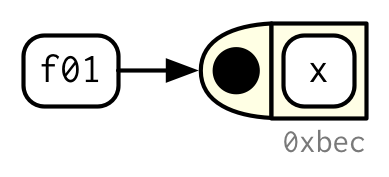
\includegraphics{diagrams/functions/first-class} \end{center}

匿名函數:

\begin{Shaded}
\begin{Highlighting}[]
\KeywordTok{lapply}\NormalTok{(mtcars, }\ControlFlowTok{function}\NormalTok{(x) }\KeywordTok{length}\NormalTok{(}\KeywordTok{unique}\NormalTok{(x)))}
\KeywordTok{Filter}\NormalTok{(}\ControlFlowTok{function}\NormalTok{(x) }\OperatorTok{!}\KeywordTok{is.numeric}\NormalTok{(x), mtcars)}
\KeywordTok{integrate}\NormalTok{(}\ControlFlowTok{function}\NormalTok{(x) }\KeywordTok{sin}\NormalTok{(x) }\OperatorTok{^}\StringTok{ }\DecValTok{2}\NormalTok{, }\DecValTok{0}\NormalTok{, pi)}
\end{Highlighting}
\end{Shaded}

在list中,也可以放入:

\begin{Shaded}
\begin{Highlighting}[]
\NormalTok{funs <-}\StringTok{ }\KeywordTok{list}\NormalTok{(}
  \DataTypeTok{half =} \ControlFlowTok{function}\NormalTok{(x) x }\OperatorTok{/}\StringTok{ }\DecValTok{2}\NormalTok{,}
  \DataTypeTok{double =} \ControlFlowTok{function}\NormalTok{(x) x }\OperatorTok{*}\StringTok{ }\DecValTok{2}
\NormalTok{)}

\NormalTok{funs}\OperatorTok{$}\KeywordTok{double}\NormalTok{(}\DecValTok{10}\NormalTok{)}
\end{Highlighting}
\end{Shaded}

在R語言中,函數有叫做closure因為,R函數包含(enclose)它們的環境
environments.

\begin{Shaded}
\begin{Highlighting}[]
\KeywordTok{typeof}\NormalTok{(f01)}
\end{Highlighting}
\end{Shaded}

\subsection{Function components}\label{function-components}

1個函數有3個部分:

\begin{itemize}
\item
  \texttt{formals()}, 參數
\item
  \texttt{body()}, \{\}內部.
\item
  \texttt{environment()}, 決定函數怎樣找出變數(names)的內容。.
\end{itemize}

I'll draw functions as in the following diagram. The black dot on the
left is the environment. The two blocks to the right are the function
arguments. I won't draw the body, because it's usually large, and
doesn't help you understand the ``shape'' of the function.

\begin{center}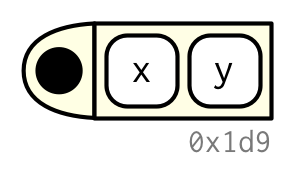
\includegraphics{diagrams/functions/components} \end{center}

The function environment always exists, but it is only printed when the
function isn't defined in the global environment.

\begin{Shaded}
\begin{Highlighting}[]
\NormalTok{f02 <-}\StringTok{ }\ControlFlowTok{function}\NormalTok{(x) \{}
  \CommentTok{# A comment}
\NormalTok{  x }\OperatorTok{^}\StringTok{ }\DecValTok{2}
\NormalTok{\}}

\KeywordTok{formals}\NormalTok{(f02)}
\end{Highlighting}
\end{Shaded}

\begin{Shaded}
\begin{Highlighting}[]
\KeywordTok{body}\NormalTok{(f02)}
\end{Highlighting}
\end{Shaded}

\begin{Shaded}
\begin{Highlighting}[]
\KeywordTok{environment}\NormalTok{(f02)}
\end{Highlighting}
\end{Shaded}

就像所以其他R的物件,函數也有很多 \texttt{attributes()}. 其中一個
``srcref'', 是 source reference的縮寫。  

\begin{Shaded}
\begin{Highlighting}[]
\KeywordTok{attr}\NormalTok{(f02, }\StringTok{"srcref"}\NormalTok{)}
\end{Highlighting}
\end{Shaded}

\subsection{Primitive functions}\label{primitive-functions}

3個組件的規則有例外,像是 Primitive functions, like \texttt{sum()} and
\texttt{{[}}, 直接調用C語言。

\begin{Shaded}
\begin{Highlighting}[]
\NormalTok{sum}
\end{Highlighting}
\end{Shaded}

\begin{Shaded}
\begin{Highlighting}[]
\StringTok{`}\DataTypeTok{[}\StringTok{`}
\end{Highlighting}
\end{Shaded}

看一下type 分別屬於 ``builtin'' or ``special'':

\begin{Shaded}
\begin{Highlighting}[]
\KeywordTok{typeof}\NormalTok{(sum)}
\end{Highlighting}
\end{Shaded}

\begin{Shaded}
\begin{Highlighting}[]
\KeywordTok{typeof}\NormalTok{(}\StringTok{`}\DataTypeTok{[}\StringTok{`}\NormalTok{)}
\end{Highlighting}
\end{Shaded}

因此, \texttt{formals()}, \texttt{body()}, and \texttt{environment()}
都回傳 \texttt{NULL}:

\begin{Shaded}
\begin{Highlighting}[]
\KeywordTok{formals}\NormalTok{(sum)}
\end{Highlighting}
\end{Shaded}

\begin{Shaded}
\begin{Highlighting}[]
\KeywordTok{body}\NormalTok{(sum)}
\end{Highlighting}
\end{Shaded}

\begin{Shaded}
\begin{Highlighting}[]
\KeywordTok{environment}\NormalTok{(sum)}
\end{Highlighting}
\end{Shaded}

這些所謂的原始函數,只存在於基本套件(base packages) 。.

\subsection{Exercises}\label{exercises}

\begin{enumerate}
\def\labelenumi{\arabic{enumi}.}
\item
  Given a function, like \texttt{"mean"}, \texttt{match.fun()} lets you
  find a function. Given a function, can you find its name? Why doesn't
  that make sense in R?
\item
  It's possible (although typically not useful) to call an anonymous
  function. Which of the two approaches below is correct? Why?

\begin{Shaded}
\begin{Highlighting}[]
\ControlFlowTok{function}\NormalTok{(x) }\DecValTok{3}\NormalTok{()}
\end{Highlighting}
\end{Shaded}

\begin{Shaded}
\begin{Highlighting}[]
\NormalTok{(}\ControlFlowTok{function}\NormalTok{(x) }\DecValTok{3}\NormalTok{)()}
\end{Highlighting}
\end{Shaded}
\item
  A good rule of thumb is that an anonymous function should fit on one
  line and shouldn't need to use \texttt{\{\}}. Review your code. Where
  could you have used an anonymous function instead of a named function?
  Where should you have used a named function instead of an anonymous
  function?
\item
  What function allows you to tell if an object is a function? What
  function allows you to tell if a function is a primitive function?
\item
  This code makes a list of all functions in the base package.

\begin{Shaded}
\begin{Highlighting}[]
\NormalTok{objs <-}\StringTok{ }\KeywordTok{mget}\NormalTok{(}\KeywordTok{ls}\NormalTok{(}\StringTok{"package:base"}\NormalTok{), }\DataTypeTok{inherits =} \OtherTok{TRUE}\NormalTok{)}
\NormalTok{funs <-}\StringTok{ }\KeywordTok{Filter}\NormalTok{(is.function, objs)}
\end{Highlighting}
\end{Shaded}

  Use it to answer the following questions:

  \begin{enumerate}
  \def\labelenumii{\alph{enumii}.}
  \item
    Which base function has the most arguments?
  \item
    How many base functions have no arguments? What's special about
    those functions?
  \item
    How could you adapt the code to find all primitive functions?
  \end{enumerate}
\item
  What are the three important components of a function?
\item
  When does printing a function not show the environment it was created
  in?
\end{enumerate}

\section{Lexical scoping}\label{lexical-scoping}

In {[}Names and values{]}, we discussed assignment, the act of binding a
name to a value. Here we'll discuss \textbf{scoping}, the act of finding
the value associated with a name.

下面的執行結果傳回10還是20?\footnote{\texttt{20}.}

\begin{Shaded}
\begin{Highlighting}[]
\NormalTok{x <-}\StringTok{ }\DecValTok{10}
\NormalTok{g01 <-}\StringTok{ }\ControlFlowTok{function}\NormalTok{() \{}
\NormalTok{  x <-}\StringTok{ }\DecValTok{20}
\NormalTok{  x}
\NormalTok{\}}

\KeywordTok{g01}\NormalTok{()}
\end{Highlighting}
\end{Shaded}

了解範圍規則,有助於函數的模組開發,甚至有助於將R翻譯到其他語言。

\emph{lexical scoping} \footnote{Functions that automatically quote one
  or more arguments (sometimes called NSE functions) can override the
  default scoping rules to implement other varieties of scoping. You'll
  learn more about that in \protect\hyperlink{meta}{metaprogramming}.}:
it looks up the values of names based on how a function is defined, not
how it is called. ``Lexical'' here is not the English adjective
``relating to words or a vocabulary''. It's a technical CS term that
tells us that the scoping rules use a parse-time, rather than a run-time
structure.

R的's lexical scoping 遵循4個主要規則::

\begin{itemize}
\tightlist
\item
  Name masking
\item
  Functions vs.~variables
\item
  A fresh start
\item
  Dynamic lookup
\end{itemize}

\subsection{Name masking}\label{name-masking}

內部範圍的宣告(第一次使用)覆蓋外部範圍的宣告。.

\begin{Shaded}
\begin{Highlighting}[]
\NormalTok{x <-}\StringTok{ }\DecValTok{10}
\NormalTok{y <-}\StringTok{ }\DecValTok{20}
\NormalTok{g02 <-}\StringTok{ }\ControlFlowTok{function}\NormalTok{() \{}
\NormalTok{  x <-}\StringTok{ }\DecValTok{1}
\NormalTok{  y <-}\StringTok{ }\DecValTok{2}
  \KeywordTok{c}\NormalTok{(x, y)}
\NormalTok{\}}
\KeywordTok{g02}\NormalTok{()}
\end{Highlighting}
\end{Shaded}

如果在內部宣告找不到,就找外一層,一直到global environment。

\begin{Shaded}
\begin{Highlighting}[]
\NormalTok{x <-}\StringTok{ }\DecValTok{2}
\NormalTok{g03 <-}\StringTok{ }\ControlFlowTok{function}\NormalTok{() \{}
\NormalTok{  y <-}\StringTok{ }\DecValTok{1}
  \KeywordTok{c}\NormalTok{(x, y)}
\NormalTok{\}}
\KeywordTok{g03}\NormalTok{()}
\end{Highlighting}
\end{Shaded}

上面的規則仍然適用於函數中的函數.

測試:下面的R程式會有甚麼結果 ? \footnote{\texttt{g04()} returns
  \texttt{c(1,\ 2,\ 3)}.}

\begin{Shaded}
\begin{Highlighting}[]
\NormalTok{x <-}\StringTok{ }\DecValTok{1}
\NormalTok{g04 <-}\StringTok{ }\ControlFlowTok{function}\NormalTok{() \{}
\NormalTok{  y <-}\StringTok{ }\DecValTok{2}
\NormalTok{  i <-}\StringTok{ }\ControlFlowTok{function}\NormalTok{() \{}
\NormalTok{    z <-}\StringTok{ }\DecValTok{3}
    \KeywordTok{c}\NormalTok{(x, y, z)}
\NormalTok{  \}}
  \KeywordTok{i}\NormalTok{()}
\NormalTok{\}}
\KeywordTok{g04}\NormalTok{()}
\end{Highlighting}
\end{Shaded}

同樣也適用於建立函數的函數( \textbf{closures}).參考 {[}closures{]};
這裡只是用來說明上述規則的使用。 \texttt{g05()},
傳回函數,猜猜執行結果?\footnote{\texttt{g06()} returns
  \texttt{c(10,\ 2)}.}

\begin{Shaded}
\begin{Highlighting}[]
\NormalTok{x <-}\StringTok{ }\DecValTok{10}
\NormalTok{y <-}\StringTok{ }\DecValTok{20}

\NormalTok{g05 <-}\StringTok{ }\ControlFlowTok{function}\NormalTok{() \{}
\NormalTok{  y <-}\StringTok{ }\DecValTok{2}
  \ControlFlowTok{function}\NormalTok{() \{}
    \KeywordTok{c}\NormalTok{(x, y)}
\NormalTok{  \}}
\NormalTok{\}}
\NormalTok{g06 <-}\StringTok{ }\KeywordTok{g05}\NormalTok{()}
\KeywordTok{g06}\NormalTok{()}
\end{Highlighting}
\end{Shaded}

This seems a little magical: how does R know what the value of
\texttt{y} is after \texttt{j()} has returned? It works because
\texttt{k} preserves the environment in which it was defined and because
the environment includes the value of \texttt{y}. You'll learn more
about how environments work in
\protect\hyperlink{environments}{Environments}.

\subsection{Functions vs.~variables}\label{functions-vs.variables}

既然函數也只是普通的物件,那麼同樣的名稱尋找規則也適用於函數:這個例子中,g07在外部和內部皆有定義。

\begin{Shaded}
\begin{Highlighting}[]
\NormalTok{g07 <-}\StringTok{ }\ControlFlowTok{function}\NormalTok{(x) x }\OperatorTok{+}\StringTok{ }\DecValTok{1}
\NormalTok{g08 <-}\StringTok{ }\ControlFlowTok{function}\NormalTok{() \{}
\NormalTok{  g07 <-}\StringTok{ }\ControlFlowTok{function}\NormalTok{(x) x }\OperatorTok{+}\StringTok{ }\DecValTok{100}
  \KeywordTok{g07}\NormalTok{(}\DecValTok{10}\NormalTok{)}
\NormalTok{\}}
\KeywordTok{g08}\NormalTok{()}
\end{Highlighting}
\end{Shaded}

但是如果同一個名稱,在不同範圍有不一樣的型態呢?例如g9一個是變數,一個是函數:

\begin{Shaded}
\begin{Highlighting}[]
\NormalTok{g09 <-}\StringTok{ }\ControlFlowTok{function}\NormalTok{(x) x }\OperatorTok{+}\StringTok{ }\DecValTok{100}
\NormalTok{g10 <-}\StringTok{ }\ControlFlowTok{function}\NormalTok{() \{}
\NormalTok{  g09 <-}\StringTok{ }\DecValTok{10}
  \KeywordTok{g09}\NormalTok{(g09)}
\NormalTok{\}}
\KeywordTok{g10}\NormalTok{()}
\end{Highlighting}
\end{Shaded}

一般來講,上面的用法在語法上是沒問題,但是最好避免。

\hypertarget{fresh-start}{\subsection{A fresh start}\label{fresh-start}}

第一次執行和第二次執行有甚麼不同?\footnote{\texttt{g11()}
  每次被調用都是傳回 \texttt{1}。.}

函數 \texttt{exists(x)} :會尋找變數名稱x是否存在,存在則無回
\texttt{TRUE},否則傳回 \texttt{FALSE}.)

\begin{Shaded}
\begin{Highlighting}[]
\NormalTok{g11 <-}\StringTok{ }\ControlFlowTok{function}\NormalTok{() \{}
  \ControlFlowTok{if}\NormalTok{ (}\OperatorTok{!}\KeywordTok{exists}\NormalTok{(}\StringTok{"a"}\NormalTok{)) \{}
\NormalTok{    a <-}\StringTok{ }\DecValTok{1}
\NormalTok{  \} }\ControlFlowTok{else}\NormalTok{ \{}
\NormalTok{    a <-}\StringTok{ }\NormalTok{a }\OperatorTok{+}\StringTok{ }\DecValTok{1}
\NormalTok{  \}}
\NormalTok{  a}
\NormalTok{\}}

\KeywordTok{g11}\NormalTok{()}
\KeywordTok{g11}\NormalTok{()}
\end{Highlighting}
\end{Shaded}

每次執行的時候,一個新的environment會被建立,用來主導函數的執行。
\ref{stateful-funs}.)

\subsection{Dynamic lookup}\label{dynamic-lookup}

Lexical scoping determines where to look for values, not when to look
for them. R looks for values when the function is run, not when it's
created. This means that the output of a function can differ depending
on objects outside its environment:

\begin{Shaded}
\begin{Highlighting}[]
\NormalTok{g12 <-}\StringTok{ }\ControlFlowTok{function}\NormalTok{() x }\OperatorTok{+}\StringTok{ }\DecValTok{1}
\NormalTok{x <-}\StringTok{ }\DecValTok{15}
\KeywordTok{g12}\NormalTok{()}
\end{Highlighting}
\end{Shaded}

\begin{Shaded}
\begin{Highlighting}[]
\NormalTok{x <-}\StringTok{ }\DecValTok{20}
\KeywordTok{g12}\NormalTok{()}
\end{Highlighting}
\end{Shaded}

This behaviour can be quite annoying. If you make a spelling mistake in
your code, you won't get an error when you create the function, and you
might not even get one when you run the function, depending on what
variables are defined in the global environment.

One way to detect this problem is to use
\texttt{codetools::findGlobals()}. This function lists all the external
dependencies (unbound symbols) within a function:

\begin{Shaded}
\begin{Highlighting}[]
\NormalTok{codetools}\OperatorTok{::}\KeywordTok{findGlobals}\NormalTok{(g12)}
\end{Highlighting}
\end{Shaded}

Another way to solve the problem would be to manually change the
environment of the function to the \texttt{emptyenv()}, an environment
which contains nothing:

\begin{Shaded}
\begin{Highlighting}[]
\KeywordTok{environment}\NormalTok{(g12) <-}\StringTok{ }\KeywordTok{emptyenv}\NormalTok{()}
\KeywordTok{g12}\NormalTok{()}
\end{Highlighting}
\end{Shaded}

Both of these approaches reveal why this undesirable behaviour exists: R
relies on lexical scoping to find \emph{everything}, even the \texttt{+}
operator. This provides a rather beautiful simplicity to R's scoping
rules.

\subsection{Exercises}\label{exercises-1}

\begin{enumerate}
\def\labelenumi{\arabic{enumi}.}
\item
  What does the following code return? Why? Describe how each of the
  three \texttt{c}'s is interpreted.

\begin{Shaded}
\begin{Highlighting}[]
\NormalTok{c <-}\StringTok{ }\DecValTok{10}
\KeywordTok{c}\NormalTok{(}\DataTypeTok{c =}\NormalTok{ c)}
\end{Highlighting}
\end{Shaded}
\item
  What are the four principles that govern how R looks for values?
\item
  What does the following function return? Make a prediction before
  running the code yourself.

\begin{Shaded}
\begin{Highlighting}[]
\NormalTok{f <-}\StringTok{ }\ControlFlowTok{function}\NormalTok{(x) \{}
\NormalTok{  f <-}\StringTok{ }\ControlFlowTok{function}\NormalTok{(x) \{}
\NormalTok{    f <-}\StringTok{ }\ControlFlowTok{function}\NormalTok{() \{}
\NormalTok{      x }\OperatorTok{^}\StringTok{ }\DecValTok{2}
\NormalTok{    \}}
    \KeywordTok{f}\NormalTok{() }\OperatorTok{+}\StringTok{ }\DecValTok{1}
\NormalTok{  \}}
  \KeywordTok{f}\NormalTok{(x) }\OperatorTok{*}\StringTok{ }\DecValTok{2}
\NormalTok{\}}
\KeywordTok{f}\NormalTok{(}\DecValTok{10}\NormalTok{)}
\end{Highlighting}
\end{Shaded}
\end{enumerate}

\section{Lazy evaluation}\label{lazy-evaluation}

In R, function arguments are \textbf{lazily evaluated}: they're only
evaluated if accessed. For example, this code doesn't generate an error
because \texttt{x} is never used:

\begin{Shaded}
\begin{Highlighting}[]
\NormalTok{h01 <-}\StringTok{ }\ControlFlowTok{function}\NormalTok{(x) \{}
  \DecValTok{10}
\NormalTok{\}}
\KeywordTok{h01}\NormalTok{(}\KeywordTok{stop}\NormalTok{(}\StringTok{"This is an error!"}\NormalTok{))}
\end{Highlighting}
\end{Shaded}

This is an important feature because it allows you to do things like
include potentially expensive computations in function arguments that
will only be evaluated if needed.

\subsection{Forcing evaluation}\label{forcing-evaluation}

To \textbf{compel} the evaluation of an argument, use \texttt{force()}:

\begin{Shaded}
\begin{Highlighting}[]
\NormalTok{h02 <-}\StringTok{ }\ControlFlowTok{function}\NormalTok{(x) \{}
  \KeywordTok{force}\NormalTok{(x)}
  \DecValTok{10}
\NormalTok{\}}
\KeywordTok{h02}\NormalTok{(}\KeywordTok{stop}\NormalTok{(}\StringTok{"This is an error!"}\NormalTok{))}
\end{Highlighting}
\end{Shaded}

It is usually not necessary to force evaluation. It's needed primarily
for certain functional programming techniques which we'll cover in
detail in {[}function operators{]}. Here, I want to show you the basic
issue.

Take this small but surprisingly tricky function. It takes a single
argument \texttt{x}, and returns a function that returns \texttt{x} when
called.

\begin{Shaded}
\begin{Highlighting}[]
\NormalTok{capture1 <-}\StringTok{ }\ControlFlowTok{function}\NormalTok{(x) \{}
  \ControlFlowTok{function}\NormalTok{() \{}
\NormalTok{    x}
\NormalTok{  \}}
\NormalTok{\}}
\end{Highlighting}
\end{Shaded}

There's a subtle issue with this function: the value of \texttt{x} will
be captured not when you call \texttt{capture()}, but when you call the
function that \texttt{capture()} returns:

\begin{Shaded}
\begin{Highlighting}[]
\NormalTok{x <-}\StringTok{ }\DecValTok{10}
\NormalTok{h03 <-}\StringTok{ }\KeywordTok{capture1}\NormalTok{(x)}
\NormalTok{h04 <-}\StringTok{ }\KeywordTok{capture1}\NormalTok{(x)}

\KeywordTok{h03}\NormalTok{()}
\end{Highlighting}
\end{Shaded}

\begin{Shaded}
\begin{Highlighting}[]
\NormalTok{x <-}\StringTok{ }\DecValTok{20}
\KeywordTok{h04}\NormalTok{()}
\end{Highlighting}
\end{Shaded}

Even more confusingly this only happens once: the value is locked in
after you have called \texttt{h03()}/\texttt{h04()} for the first time.

\begin{Shaded}
\begin{Highlighting}[]
\NormalTok{x <-}\StringTok{ }\DecValTok{30}
\KeywordTok{h03}\NormalTok{()}
\end{Highlighting}
\end{Shaded}

\begin{Shaded}
\begin{Highlighting}[]
\KeywordTok{h04}\NormalTok{()}
\end{Highlighting}
\end{Shaded}

This behaviour is a consequence of lazy evaluation. The \texttt{x}
argument is evaluated once \texttt{h03()}/\texttt{h04()} is called, and
then its value is cached. We can avoid the confusion by forcing
\texttt{x}:

\begin{Shaded}
\begin{Highlighting}[]
\NormalTok{capture2 <-}\StringTok{ }\ControlFlowTok{function}\NormalTok{(x) \{}
  \KeywordTok{force}\NormalTok{(x)}
  
  \ControlFlowTok{function}\NormalTok{() \{}
\NormalTok{    x}
\NormalTok{  \}}
\NormalTok{\}}

\NormalTok{x <-}\StringTok{ }\DecValTok{10}
\NormalTok{h05 <-}\StringTok{ }\KeywordTok{capture2}\NormalTok{(x)}

\NormalTok{x <-}\StringTok{ }\DecValTok{20}
\KeywordTok{h05}\NormalTok{()}
\end{Highlighting}
\end{Shaded}

\subsection{Promises}\label{promises}

\}

Lazy evaluation is powered by a data structure called a
\textbf{promise}, or (less commonly) a thunk. We'll come back to this
data structure in \protect\hyperlink{meta}{metaprogramming} because it's
one of the features of R that makes it most interesting as a programming
language.

A promise has three components:

\begin{itemize}
\item
  The expression, like \texttt{x\ +\ y} which gives rise to the delayed
  computation.
\item
  The environment where the expression should be evaluated.
\item
  The value, which is computed and cached when the promise is first
  accessed by evaluating the expression in the specified environment.
\end{itemize}

The value cache ensures that accessing the promise multiple times always
returns the same value. For example, you can see in the following code
that \texttt{runif(1)} is only evaluated once:

\begin{Shaded}
\begin{Highlighting}[]
\NormalTok{h06 <-}\StringTok{ }\ControlFlowTok{function}\NormalTok{(x) \{ }
  \KeywordTok{c}\NormalTok{(x, x, x)  }
\NormalTok{\}}

\KeywordTok{h06}\NormalTok{(}\KeywordTok{runif}\NormalTok{(}\DecValTok{1}\NormalTok{))}
\end{Highlighting}
\end{Shaded}

You can also create promises ``by hand'' using \texttt{delayedAssign()}:

\begin{Shaded}
\begin{Highlighting}[]
\KeywordTok{delayedAssign}\NormalTok{(}\StringTok{"x"}\NormalTok{, \{}\KeywordTok{print}\NormalTok{(}\StringTok{"Executing code"}\NormalTok{); }\KeywordTok{runif}\NormalTok{(}\DecValTok{1}\NormalTok{)\})}
\NormalTok{x}
\end{Highlighting}
\end{Shaded}

\begin{Shaded}
\begin{Highlighting}[]
\NormalTok{x}
\end{Highlighting}
\end{Shaded}

You'll see this idea again in
\protect\hyperlink{advanced-bindings}{advanced bindings}.

\subsection{Default arguments}\label{default-arguments}

Thanks to lazy evaluation, default value can be defined in terms of
other arguments, or even in terms of variables defined later in the
function:

\begin{Shaded}
\begin{Highlighting}[]
\NormalTok{h07 <-}\StringTok{ }\ControlFlowTok{function}\NormalTok{(}\DataTypeTok{x =} \DecValTok{1}\NormalTok{, }\DataTypeTok{y =}\NormalTok{ x }\OperatorTok{*}\StringTok{ }\DecValTok{2}\NormalTok{, }\DataTypeTok{z =}\NormalTok{ a }\OperatorTok{+}\StringTok{ }\NormalTok{b) \{}
\NormalTok{  a <-}\StringTok{ }\DecValTok{10}
\NormalTok{  b <-}\StringTok{ }\DecValTok{100}
  
  \KeywordTok{c}\NormalTok{(x, y, z)}
\NormalTok{\}}

\KeywordTok{h07}\NormalTok{()}
\end{Highlighting}
\end{Shaded}

Many base R functions use this technique, but I don't recommend it. It
makes code harder to understand because it requires that you know
exactly \emph{when} default arguments are evaluated in order to predict
\emph{what} they will evaluate to.

The evaluation environment is slightly different for default and user
supplied arguments, as default arguments are evaluated inside the
function. This means that seemingly identical calls can yield different
results. It's easiest to see this with an extreme example:

\begin{Shaded}
\begin{Highlighting}[]
\NormalTok{h08 <-}\StringTok{ }\ControlFlowTok{function}\NormalTok{(}\DataTypeTok{x =} \KeywordTok{ls}\NormalTok{()) \{}
\NormalTok{  a <-}\StringTok{ }\DecValTok{1}
\NormalTok{  x}
\NormalTok{\}}

\CommentTok{# ls() evaluated inside f:}
\KeywordTok{h08}\NormalTok{()}
\CommentTok{#> [1] "a" "x"}

\CommentTok{# ls() evaluated in global environment:}
\KeywordTok{h08}\NormalTok{(}\KeywordTok{ls}\NormalTok{())}
\CommentTok{#> [1] "f"}
\end{Highlighting}
\end{Shaded}

\subsection{Missing arguments}\label{missing-arguments}

If an argument has a default, you can determine if the value comes from
the user or the default with \texttt{missing()}:

\begin{Shaded}
\begin{Highlighting}[]
\NormalTok{h09 <-}\StringTok{ }\ControlFlowTok{function}\NormalTok{(}\DataTypeTok{x =} \DecValTok{10}\NormalTok{) \{}
  \KeywordTok{list}\NormalTok{(}\KeywordTok{missing}\NormalTok{(x), x)}
\NormalTok{\}}
\KeywordTok{str}\NormalTok{(}\KeywordTok{h09}\NormalTok{())}
\end{Highlighting}
\end{Shaded}

\begin{Shaded}
\begin{Highlighting}[]
\KeywordTok{str}\NormalTok{(}\KeywordTok{h09}\NormalTok{(}\DecValTok{10}\NormalTok{))}
\end{Highlighting}
\end{Shaded}

\texttt{missing()} is best used sparingly. Take \texttt{sample()}, for
example. How many arguments are required?

\begin{Shaded}
\begin{Highlighting}[]
\KeywordTok{args}\NormalTok{(sample)}
\end{Highlighting}
\end{Shaded}

It looks like both \texttt{x} and \texttt{size} are required, but in
fact \texttt{sample()} uses \texttt{missing()} to provide a default for
\texttt{size} if it's not supplied. If I was to rewrite sample
myself\footnote{Note that this only implements one way of calling
  \texttt{sample()}: you can also call it with a single integer, like
  \texttt{sample(10)}. This unfortunately makes \texttt{sample()} prone
  to silent errors in situations like \texttt{sample(x{[}i{]})}.}, I'd
use an explicit \texttt{NULL} to indicate that \texttt{size} can be
supplied, but it's not required:

\begin{Shaded}
\begin{Highlighting}[]
\NormalTok{sample <-}\StringTok{ }\ControlFlowTok{function}\NormalTok{(x, }\DataTypeTok{size =} \OtherTok{NULL}\NormalTok{, }\DataTypeTok{replace =} \OtherTok{FALSE}\NormalTok{, }\DataTypeTok{prob =} \OtherTok{NULL}\NormalTok{) \{}
  \ControlFlowTok{if}\NormalTok{ (}\KeywordTok{is.null}\NormalTok{(size)) \{}
\NormalTok{    size <-}\StringTok{ }\KeywordTok{length}\NormalTok{(x)}
\NormalTok{  \}}
  
\NormalTok{  x[}\KeywordTok{sample.int}\NormalTok{(}\KeywordTok{length}\NormalTok{(x), size, }\DataTypeTok{replace =}\NormalTok{ replace, }\DataTypeTok{prob =}\NormalTok{ prob)]}
\NormalTok{\}}
\end{Highlighting}
\end{Shaded}

You can make that pattern even simpler with a small helper. The infix
\texttt{\%\textbar{}\textbar{}\%} function uses the LHS if it's not
null, otherwise it uses the RHS:

\begin{Shaded}
\begin{Highlighting}[]
\StringTok{`}\DataTypeTok\StringTok{`}\NormalTok{ <-}\StringTok{ }\ControlFlowTok{function}\NormalTok{(lhs, rhs) \{}
  \ControlFlowTok{if}\NormalTok{ (}\OperatorTok{!}\KeywordTok{is.null}\NormalTok{(lhs)) \{}
\NormalTok{    lhs}
\NormalTok{  \} }\ControlFlowTok{else}\NormalTok{ \{}
\NormalTok{    rhs}
\NormalTok{  \}}
\NormalTok{\}}

\NormalTok{sample <-}\StringTok{ }\ControlFlowTok{function}\NormalTok{(x, }\DataTypeTok{size =} \OtherTok{NULL}\NormalTok{, }\DataTypeTok{replace =} \OtherTok{FALSE}\NormalTok{, }\DataTypeTok{prob =} \OtherTok{NULL}\NormalTok{) \{}
\NormalTok{  size <-}\StringTok{ }\NormalTok{size }\OperatorTok\StringTok{ }\KeywordTok{length}\NormalTok{(x)}
\NormalTok{  x[}\KeywordTok{sample.int}\NormalTok{(}\KeywordTok{length}\NormalTok{(x), size, }\DataTypeTok{replace =}\NormalTok{ replace, }\DataTypeTok{prob =}\NormalTok{ prob)]}
\NormalTok{\}}
\end{Highlighting}
\end{Shaded}

Because of lazy evaluation, you don't need to worry about unnecessary
computation: the RHS of \texttt{\%\textbar{}\textbar{}\%} will only be
evaluated if the LHS is null.

\subsection{Exercises}\label{exercises-2}

\begin{enumerate}
\def\labelenumi{\arabic{enumi}.}
\item
  What important property of \texttt{\&\&} make \texttt{x\_ok()} work?

\begin{Shaded}
\begin{Highlighting}[]
\NormalTok{x_ok <-}\StringTok{ }\ControlFlowTok{function}\NormalTok{(x) \{}
  \OperatorTok{!}\KeywordTok{is.null}\NormalTok{(x) }\OperatorTok{&&}\StringTok{ }\KeywordTok{length}\NormalTok{(x) }\OperatorTok{==}\StringTok{ }\DecValTok{1} \OperatorTok{&&}\StringTok{ }\NormalTok{x }\OperatorTok{>}\StringTok{ }\DecValTok{0}
\NormalTok{\}}

\KeywordTok{x_ok}\NormalTok{(}\OtherTok{NULL}\NormalTok{)}
\end{Highlighting}
\end{Shaded}

\begin{Shaded}
\begin{Highlighting}[]
\KeywordTok{x_ok}\NormalTok{(}\DecValTok{1}\NormalTok{)}
\end{Highlighting}
\end{Shaded}

\begin{Shaded}
\begin{Highlighting}[]
\KeywordTok{x_ok}\NormalTok{(}\DecValTok{1}\OperatorTok{:}\DecValTok{3}\NormalTok{)}
\end{Highlighting}
\end{Shaded}

  What is different with this code? Why is this behaviour undesirable
  here?

\begin{Shaded}
\begin{Highlighting}[]
\NormalTok{x_ok <-}\StringTok{ }\ControlFlowTok{function}\NormalTok{(x) \{}
  \OperatorTok{!}\KeywordTok{is.null}\NormalTok{(x) }\OperatorTok{&}\StringTok{ }\KeywordTok{length}\NormalTok{(x) }\OperatorTok{==}\StringTok{ }\DecValTok{1} \OperatorTok{&}\StringTok{ }\NormalTok{x }\OperatorTok{>}\StringTok{ }\DecValTok{0}
\NormalTok{\}}

\KeywordTok{x_ok}\NormalTok{(}\OtherTok{NULL}\NormalTok{)}
\end{Highlighting}
\end{Shaded}

\begin{Shaded}
\begin{Highlighting}[]
\KeywordTok{x_ok}\NormalTok{(}\DecValTok{1}\NormalTok{)}
\end{Highlighting}
\end{Shaded}

\begin{Shaded}
\begin{Highlighting}[]
\KeywordTok{x_ok}\NormalTok{(}\DecValTok{1}\OperatorTok{:}\DecValTok{3}\NormalTok{)}
\end{Highlighting}
\end{Shaded}
\item
  The definition of \texttt{force()} is simple:

\begin{Shaded}
\begin{Highlighting}[]
\NormalTok{force}
\end{Highlighting}
\end{Shaded}

  Why is it better to \texttt{force(x)} instead of just \texttt{x}?
\item
  What does this function return? Why? Which principle does it
  illustrate?

\begin{Shaded}
\begin{Highlighting}[]
\NormalTok{f2 <-}\StringTok{ }\ControlFlowTok{function}\NormalTok{(}\DataTypeTok{x =}\NormalTok{ z) \{}
\NormalTok{  z <-}\StringTok{ }\DecValTok{100}
\NormalTok{  x}
\NormalTok{\}}
\KeywordTok{f2}\NormalTok{()}
\end{Highlighting}
\end{Shaded}
\item
  What does this function return? Why? Which principle does it
  illustrate?

\begin{Shaded}
\begin{Highlighting}[]
\NormalTok{y <-}\StringTok{ }\DecValTok{10}
\NormalTok{f1 <-}\StringTok{ }\ControlFlowTok{function}\NormalTok{(}\DataTypeTok{x =}\NormalTok{ \{y <-}\StringTok{ }\DecValTok{1}\NormalTok{; }\DecValTok{2}\NormalTok{\}, }\DataTypeTok{y =} \DecValTok{0}\NormalTok{) \{}
  \KeywordTok{c}\NormalTok{(x, y)}
\NormalTok{\}}
\KeywordTok{f1}\NormalTok{()}
\NormalTok{y}
\end{Highlighting}
\end{Shaded}
\item
  In \texttt{hist()}, the default value of \texttt{xlim} is
  \texttt{range(breaks)}, the default value for \texttt{breaks} is
  \texttt{"Sturges"}, and

\begin{Shaded}
\begin{Highlighting}[]
\KeywordTok{range}\NormalTok{(}\StringTok{"Sturges"}\NormalTok{)}
\end{Highlighting}
\end{Shaded}

  Explain how \texttt{hist()} works to get a correct \texttt{xlim}
  value.
\item
  Explain why this function works. Why is it confusing?

\begin{Shaded}
\begin{Highlighting}[]
\NormalTok{show_time <-}\StringTok{ }\ControlFlowTok{function}\NormalTok{(}\DataTypeTok{x =} \KeywordTok{stop}\NormalTok{(}\StringTok{"Error!"}\NormalTok{)) \{}
\NormalTok{  stop <-}\StringTok{ }\ControlFlowTok{function}\NormalTok{(...) }\KeywordTok{Sys.time}\NormalTok{()}
  \KeywordTok{print}\NormalTok{(x)}
\NormalTok{\}}
\KeywordTok{show_time}\NormalTok{()}
\end{Highlighting}
\end{Shaded}
\item
  How many arguments are required when calling \texttt{library()}?
\end{enumerate}

\section{\texorpdfstring{\texttt{...}
(dot-dot-dot)}{... (dot-dot-dot)}}\label{fun-dot-dot-dot}

Functions can have a special argument \texttt{...} (pronounced
dot-dot-dot). If a function has this argument, it can take any number of
additional arguments. In other programming languages, this type of
argument is often called a varargs, or the function is said to be
variadic.

Inside a function, you can use \texttt{...} to pass those additional
arguments on to another function:

\begin{Shaded}
\begin{Highlighting}[]
\NormalTok{i01 <-}\StringTok{ }\ControlFlowTok{function}\NormalTok{(y, z) \{}
  \KeywordTok{list}\NormalTok{(}\DataTypeTok{y =}\NormalTok{ y, }\DataTypeTok{z =}\NormalTok{ z)}
\NormalTok{\}}

\NormalTok{i02 <-}\StringTok{ }\ControlFlowTok{function}\NormalTok{(x, ...) \{}
  \KeywordTok{i01}\NormalTok{(...)}
\NormalTok{\}}

\KeywordTok{str}\NormalTok{(}\KeywordTok{i02}\NormalTok{(}\DataTypeTok{x =} \DecValTok{1}\NormalTok{, }\DataTypeTok{y =} \DecValTok{2}\NormalTok{, }\DataTypeTok{z =} \DecValTok{3}\NormalTok{))}
\end{Highlighting}
\end{Shaded}

It's possible (but rarely useful) to refer to elements of \texttt{...}
by their position, using a special form:

\begin{Shaded}
\begin{Highlighting}[]
\NormalTok{i03 <-}\StringTok{ }\ControlFlowTok{function}\NormalTok{(...) \{}
  \KeywordTok{list}\NormalTok{(}\DataTypeTok{first =}\NormalTok{ ..}\DecValTok{1}\NormalTok{, }\DataTypeTok{third =}\NormalTok{ ..}\DecValTok{3}\NormalTok{)}
\NormalTok{\}}
\KeywordTok{str}\NormalTok{(}\KeywordTok{i03}\NormalTok{(}\DecValTok{1}\NormalTok{, }\DecValTok{2}\NormalTok{, }\DecValTok{3}\NormalTok{))}
\end{Highlighting}
\end{Shaded}

More often useful is \texttt{list(...)}, which evaluates the arguments
and stores them in a list:

\begin{Shaded}
\begin{Highlighting}[]
\NormalTok{i04 <-}\StringTok{ }\ControlFlowTok{function}\NormalTok{(...) \{}
  \KeywordTok{list}\NormalTok{(...)}
\NormalTok{\}}
\KeywordTok{str}\NormalTok{(}\KeywordTok{i04}\NormalTok{(}\DataTypeTok{a =} \DecValTok{1}\NormalTok{, }\DataTypeTok{b =} \DecValTok{2}\NormalTok{))}
\end{Highlighting}
\end{Shaded}

(See also \texttt{rlang::list2()} to support splicing and to silently
ignore trailing commas, and \texttt{rlang::enquos()} to capture the
unevaluated arguments, the topic of {[}quasiquotation{]}.)

There are two primary uses of \texttt{...}, both of which we'll come
back to later in the book:

\begin{itemize}
\item
  If your function takes a function as an argument, you want some way to
  pass on additional arguments to that function. In this example,
  \texttt{lapply()} uses \texttt{...} to pass \texttt{na.rm} on to
  \texttt{mean()}:

\begin{Shaded}
\begin{Highlighting}[]
\NormalTok{x <-}\StringTok{ }\KeywordTok{list}\NormalTok{(}\KeywordTok{c}\NormalTok{(}\DecValTok{1}\NormalTok{, }\DecValTok{3}\NormalTok{, }\OtherTok{NA}\NormalTok{), }\KeywordTok{c}\NormalTok{(}\DecValTok{4}\NormalTok{, }\OtherTok{NA}\NormalTok{, }\DecValTok{6}\NormalTok{))}
\KeywordTok{str}\NormalTok{(}\KeywordTok{lapply}\NormalTok{(x, mean, }\DataTypeTok{na.rm =} \OtherTok{TRUE}\NormalTok{))}
\end{Highlighting}
\end{Shaded}

  We'll come back to this technique in Section
  \ref{functional-arguments}.
\item
  If your function is an S3 generic, you need some way to allow methods
  to take arbitrary extra arguments. For example, take the
  \texttt{print()} function. There are different options for printing
  types of object, so there's no way for the print generic to prespecify
  every possible argument. Instead, it uses \texttt{...} to allow
  individual methods to have different arguments:

\begin{Shaded}
\begin{Highlighting}[]
\KeywordTok{print}\NormalTok{(}\KeywordTok{factor}\NormalTok{(letters), }\DataTypeTok{max.levels =} \DecValTok{4}\NormalTok{)}

\KeywordTok{print}\NormalTok{(y }\OperatorTok{~}\StringTok{ }\NormalTok{x, }\DataTypeTok{showEnv =} \OtherTok{TRUE}\NormalTok{)}
\end{Highlighting}
\end{Shaded}

  We'll come back to this use of \texttt{...} in Section
  \ref{s3-arguments}.
\end{itemize}

Using \texttt{...} comes with two downsides:

\begin{itemize}
\item
  When you use it to pass arguments on to another function, you have to
  carefully explain to the user where those arguments go. This makes it
  hard to understand the what you can do with functions like
  \texttt{lapply()} and \texttt{plot()}.
\item
  Any misspelled arguments will not raise an error. This makes it easy
  for typos to go unnoticed:

\begin{Shaded}
\begin{Highlighting}[]
\KeywordTok{sum}\NormalTok{(}\DecValTok{1}\NormalTok{, }\DecValTok{2}\NormalTok{, }\OtherTok{NA}\NormalTok{, }\DataTypeTok{na_rm =} \OtherTok{TRUE}\NormalTok{)}
\end{Highlighting}
\end{Shaded}
\end{itemize}

\texttt{...} is a powerful tool, but be aware of the downsides.

\subsection{Exercises}\label{exercises-3}

\begin{enumerate}
\def\labelenumi{\arabic{enumi}.}
\item
  Explain the following results:

\begin{Shaded}
\begin{Highlighting}[]
\KeywordTok{sum}\NormalTok{(}\DecValTok{1}\NormalTok{, }\DecValTok{2}\NormalTok{, }\DecValTok{3}\NormalTok{)}
\end{Highlighting}
\end{Shaded}

\begin{Shaded}
\begin{Highlighting}[]
\KeywordTok{mean}\NormalTok{(}\DecValTok{1}\NormalTok{, }\DecValTok{2}\NormalTok{, }\DecValTok{3}\NormalTok{)}
\end{Highlighting}
\end{Shaded}

\begin{Shaded}
\begin{Highlighting}[]
\KeywordTok{sum}\NormalTok{(}\DecValTok{1}\NormalTok{, }\DecValTok{2}\NormalTok{, }\DecValTok{3}\NormalTok{, }\DataTypeTok{na.omit =} \OtherTok{TRUE}\NormalTok{)}
\end{Highlighting}
\end{Shaded}

\begin{Shaded}
\begin{Highlighting}[]
\KeywordTok{mean}\NormalTok{(}\DecValTok{1}\NormalTok{, }\DecValTok{2}\NormalTok{, }\DecValTok{3}\NormalTok{, }\DataTypeTok{na.omit =} \OtherTok{TRUE}\NormalTok{)}
\end{Highlighting}
\end{Shaded}
\item
  In the following call, explain how to find the documentation for the
  named arguments in the following function call:

\begin{Shaded}
\begin{Highlighting}[]
\KeywordTok{plot}\NormalTok{(}\DecValTok{1}\OperatorTok{:}\DecValTok{10}\NormalTok{, }\DataTypeTok{col =} \StringTok{"red"}\NormalTok{, }\DataTypeTok{pch =} \DecValTok{20}\NormalTok{, }\DataTypeTok{xlab =} \StringTok{"x"}\NormalTok{, }\DataTypeTok{col.lab =} \StringTok{"blue"}\NormalTok{)}
\end{Highlighting}
\end{Shaded}

  \begin{center}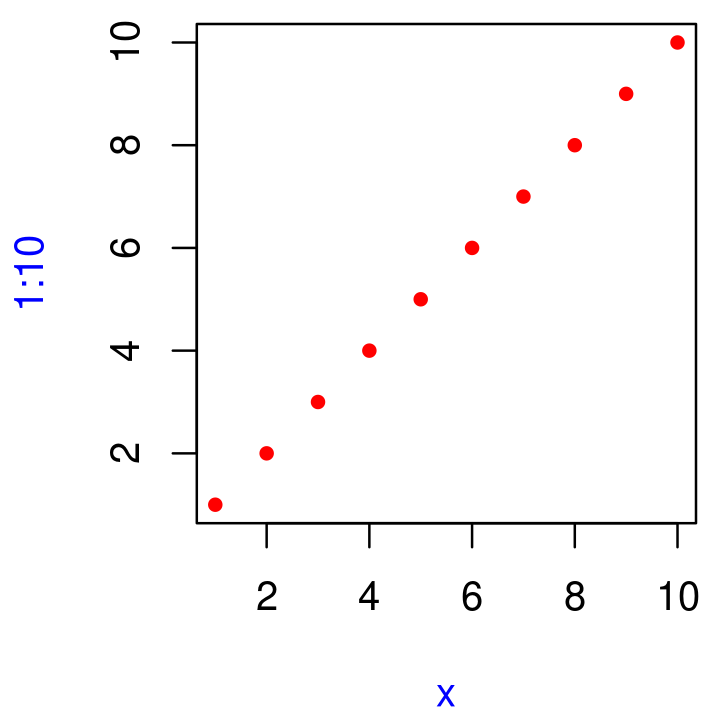
\includegraphics[width=0.7\linewidth]{rmi_copy_test_files/figure-latex/unnamed-chunk-243-1} \end{center}
\item
  Why does \texttt{plot(1:10,\ col\ =\ "red")} only colour the points,
  not the axes or labels? Read the source code of
  \texttt{plot.default()} to find out.
\end{enumerate}

\section{Exiting a function}\label{exiting-a-function}

Most functions exit in one of two ways\footnote{Functions can exit in
  other more esoteric ways like signalling a condition that is caught by
  an exiting handler, invoking a restart, or pressing ``Q'' in an
  interactive browser.}: either returning a value, indicating successful
completion, or throwing an error, indicating failure. This section
describes return values (implicit vs.~explicit; visible vs.~invisible),
briefly discusses errors, and introduces exit handlers, which allow you
to run code when a function exits, regardless of how it exits.

\subsection{Implicit vs.~explict
returns}\label{implicit-vs.explict-returns}

There are two ways that a function can return a value:

\begin{itemize}
\item
  Implicitly, where the last evaluated expression becomes the return
  value:

\begin{Shaded}
\begin{Highlighting}[]
\NormalTok{j01 <-}\StringTok{ }\ControlFlowTok{function}\NormalTok{(x) \{}
  \ControlFlowTok{if}\NormalTok{ (x }\OperatorTok{<}\StringTok{ }\DecValTok{10}\NormalTok{) \{}
    \DecValTok{0}
\NormalTok{  \} }\ControlFlowTok{else}\NormalTok{ \{}
    \DecValTok{10}
\NormalTok{  \}}
\NormalTok{\}}
\KeywordTok{f}\NormalTok{(}\DecValTok{5}\NormalTok{)}
\end{Highlighting}
\end{Shaded}

\begin{Shaded}
\begin{Highlighting}[]
\KeywordTok{f}\NormalTok{(}\DecValTok{15}\NormalTok{)}
\end{Highlighting}
\end{Shaded}
\item
  Explicitly, by calling \texttt{return()}:

\begin{Shaded}
\begin{Highlighting}[]
\NormalTok{j02 <-}\StringTok{ }\ControlFlowTok{function}\NormalTok{(x) \{}
  \ControlFlowTok{if}\NormalTok{ (x }\OperatorTok{<}\StringTok{ }\DecValTok{10}\NormalTok{) \{}
    \KeywordTok{return}\NormalTok{(}\DecValTok{0}\NormalTok{)}
\NormalTok{  \} }\ControlFlowTok{else}\NormalTok{ \{}
    \KeywordTok{return}\NormalTok{(}\DecValTok{10}\NormalTok{)}
\NormalTok{  \}}
\NormalTok{\}}
\end{Highlighting}
\end{Shaded}
\end{itemize}

\subsection{Invisible values}\label{invisible-values}

Most functions return visibly: calling the function in an interactive
context causes the result to be automatically printed.

\begin{Shaded}
\begin{Highlighting}[]
\NormalTok{j03 <-}\StringTok{ }\ControlFlowTok{function}\NormalTok{() }\DecValTok{1}
\KeywordTok{j03}\NormalTok{()}
\end{Highlighting}
\end{Shaded}

However, it's also possible to return an \texttt{invisible()} value,
which is not automatically printed.

\begin{Shaded}
\begin{Highlighting}[]
\NormalTok{j04 <-}\StringTok{ }\ControlFlowTok{function}\NormalTok{() }\KeywordTok{invisible}\NormalTok{(}\DecValTok{1}\NormalTok{)}
\KeywordTok{j04}\NormalTok{()}
\end{Highlighting}
\end{Shaded}

You can verify that the value exists either by explicitly printing it or
by wrapping in parentheses:

\begin{Shaded}
\begin{Highlighting}[]
\KeywordTok{print}\NormalTok{(}\KeywordTok{j04}\NormalTok{())}
\end{Highlighting}
\end{Shaded}

\begin{Shaded}
\begin{Highlighting}[]
\NormalTok{(}\KeywordTok{j04}\NormalTok{())}
\end{Highlighting}
\end{Shaded}

Alternatively, use \texttt{withVisible()} to return the value and a
visibility flag:

\begin{Shaded}
\begin{Highlighting}[]
\KeywordTok{str}\NormalTok{(}\KeywordTok{withVisible}\NormalTok{(}\KeywordTok{j04}\NormalTok{()))}
\end{Highlighting}
\end{Shaded}

The most common function that returns invisibly is
\texttt{\textless{}-}:

\begin{Shaded}
\begin{Highlighting}[]
\NormalTok{a <-}\StringTok{ }\DecValTok{2}
\NormalTok{(a <-}\StringTok{ }\DecValTok{2}\NormalTok{)}
\end{Highlighting}
\end{Shaded}

And this is what makes it possible to chain assignment:

\begin{Shaded}
\begin{Highlighting}[]
\NormalTok{a <-}\StringTok{ }\NormalTok{b <-}\StringTok{ }\NormalTok{c <-}\StringTok{ }\NormalTok{d <-}\StringTok{ }\DecValTok{2}
\end{Highlighting}
\end{Shaded}

In general, any function called primarily for its side effects (like
\texttt{\textless{}-}, \texttt{print()}, or \texttt{plot()}) should
return an invisible value (typically the value of the first argument).

\subsection{Errors}\label{errors}

If a function can not complete its assigned task, it should throw an
error with \texttt{stop()}, which immediately terminates the execution
of the function.

\begin{Shaded}
\begin{Highlighting}[]
\NormalTok{j05 <-}\StringTok{ }\ControlFlowTok{function}\NormalTok{() \{}
  \KeywordTok{stop}\NormalTok{(}\StringTok{"I'm an error"}\NormalTok{)}
  \KeywordTok{return}\NormalTok{(}\DecValTok{10}\NormalTok{)}
\NormalTok{\}}
\KeywordTok{j05}\NormalTok{()}
\end{Highlighting}
\end{Shaded}

Errors indicate that something has gone wrong, and force the user to
handle them. Some languages (like C, go, and rust) rely on special
return values to indicate problems, but in R you should always throw an
error. You'll learn more about errors, and how to handle them, in
{[}Conditions{]}.

\hypertarget{on-exit}{\subsection{Exit handlers}\label{on-exit}}

Sometimes a function needs to make a temporary change to global state
and you want to ensure those changes are restored when the function
completes. It's painful to make sure you cleanup before any explicit
return, and what happens if there's an error? Instead, you can set up an
\textbf{exiting handler} that is called when the function terminates,
regardless of whether it returns a value or throws an error.

To setup an exiting handler, call \texttt{on.exit()} with the code to be
run. It will execute when the function exits, regardless of what causes
it to exit:

\begin{Shaded}
\begin{Highlighting}[]
\NormalTok{j06 <-}\StringTok{ }\ControlFlowTok{function}\NormalTok{(x) \{}
  \KeywordTok{cat}\NormalTok{(}\StringTok{"Hello}\CharTok{\textbackslash{}n}\StringTok{"}\NormalTok{)}
  \KeywordTok{on.exit}\NormalTok{(}\KeywordTok{cat}\NormalTok{(}\StringTok{"Goodbye!}\CharTok{\textbackslash{}n}\StringTok{"}\NormalTok{), }\DataTypeTok{add =} \OtherTok{TRUE}\NormalTok{)}
  
  \ControlFlowTok{if}\NormalTok{ (x) \{}
    \KeywordTok{return}\NormalTok{(}\DecValTok{10}\NormalTok{)}
\NormalTok{  \} }\ControlFlowTok{else}\NormalTok{ \{}
    \KeywordTok{stop}\NormalTok{(}\StringTok{"Error"}\NormalTok{)}
\NormalTok{  \}}
\NormalTok{\}}

\KeywordTok{f}\NormalTok{(}\OtherTok{TRUE}\NormalTok{)}
\end{Highlighting}
\end{Shaded}

\begin{Shaded}
\begin{Highlighting}[]
\KeywordTok{f}\NormalTok{(}\OtherTok{FALSE}\NormalTok{)}
\end{Highlighting}
\end{Shaded}

::: sidebar Always set \texttt{add\ =\ TRUE} when using
\texttt{on.exit()}. If you don't, each call to \texttt{on.exit()} will
overwrite the previous exiting handler. Even when only registering a
single handler, it's good practice to set \texttt{add\ =\ TRUE} so that
you don't get an unpleasant surprise if you later add more exit handlers
:::

\texttt{on.exit()} is important because it allows you to place clean-up
actions next to actions with their cleanup operations.

\begin{Shaded}
\begin{Highlighting}[]
\NormalTok{cleanup <-}\StringTok{ }\ControlFlowTok{function}\NormalTok{(dir, code) \{}
\NormalTok{  old_dir <-}\StringTok{ }\KeywordTok{setwd}\NormalTok{(dir)}
  \KeywordTok{on.exit}\NormalTok{(}\KeywordTok{setwd}\NormalTok{(old), }\DataTypeTok{add =} \OtherTok{TRUE}\NormalTok{)}
  
\NormalTok{  old_opt <-}\StringTok{ }\KeywordTok{options}\NormalTok{(}\DataTypeTok{stringsAsFactors =} \OtherTok{FALSE}\NormalTok{)}
  \KeywordTok{on.exit}\NormalTok{(}\KeywordTok{options}\NormalTok{(old_opt), }\DataTypeTok{add =} \OtherTok{TRUE}\NormalTok{)}
\NormalTok{\}}
\end{Highlighting}
\end{Shaded}

When coupled with lazy evaluation, this leads to a very useful pattern
for running a block of code in an altered environment:

\begin{Shaded}
\begin{Highlighting}[]
\NormalTok{with_dir <-}\StringTok{ }\ControlFlowTok{function}\NormalTok{(dir, code) \{}
\NormalTok{  old <-}\StringTok{ }\KeywordTok{setwd}\NormalTok{(dir)}
  \KeywordTok{on.exit}\NormalTok{(}\KeywordTok{setwd}\NormalTok{(old), }\DataTypeTok{add =} \OtherTok{TRUE}\NormalTok{)}

  \KeywordTok{force}\NormalTok{(code)}
\NormalTok{\}}

\KeywordTok{getwd}\NormalTok{()}
\end{Highlighting}
\end{Shaded}

\begin{Shaded}
\begin{Highlighting}[]
\KeywordTok{with_dir}\NormalTok{(}\StringTok{"~"}\NormalTok{, }\KeywordTok{getwd}\NormalTok{())}
\end{Highlighting}
\end{Shaded}

See the \href{http://withr.r-lib.org}{withr package} for a collection of
functions of this nature.

In R 3.4 and prior, \texttt{on.exit()} expressions are always run in the
order in which they are created:

\begin{Shaded}
\begin{Highlighting}[]
\NormalTok{f <-}\StringTok{ }\ControlFlowTok{function}\NormalTok{() \{}
  \KeywordTok{on.exit}\NormalTok{(}\KeywordTok{message}\NormalTok{(}\StringTok{"a"}\NormalTok{), }\DataTypeTok{add =} \OtherTok{TRUE}\NormalTok{)}
  \KeywordTok{on.exit}\NormalTok{(}\KeywordTok{message}\NormalTok{(}\StringTok{"b"}\NormalTok{), }\DataTypeTok{add =} \OtherTok{TRUE}\NormalTok{)}
\NormalTok{\}}
\KeywordTok{f}\NormalTok{()}
\end{Highlighting}
\end{Shaded}

\begin{verbatim}
a
\end{verbatim}

\begin{verbatim}
b
\end{verbatim}

This can make cleanup a little tricky if some actions need to happen in
a specific order; typically you want the most recent added expression to
be run first. In R 3.5 and later, you can control this by setting
\texttt{after\ =\ FALSE}:

\begin{Shaded}
\begin{Highlighting}[]
\NormalTok{f <-}\StringTok{ }\ControlFlowTok{function}\NormalTok{() \{}
  \KeywordTok{on.exit}\NormalTok{(}\KeywordTok{message}\NormalTok{(}\StringTok{"a"}\NormalTok{), }\DataTypeTok{add =} \OtherTok{TRUE}\NormalTok{, }\DataTypeTok{after =} \OtherTok{FALSE}\NormalTok{)}
  \KeywordTok{on.exit}\NormalTok{(}\KeywordTok{message}\NormalTok{(}\StringTok{"b"}\NormalTok{), }\DataTypeTok{add =} \OtherTok{TRUE}\NormalTok{, }\DataTypeTok{after =} \OtherTok{FALSE}\NormalTok{)}
\NormalTok{\}}
\KeywordTok{f}\NormalTok{()}
\end{Highlighting}
\end{Shaded}

\begin{verbatim}
b
\end{verbatim}

\begin{verbatim}
a
\end{verbatim}

\subsection{Exercises}\label{exercises-4}

\begin{enumerate}
\def\labelenumi{\arabic{enumi}.}
\item
  What does \texttt{load()} return? Why don't you normally see these
  values?
\item
  What does \texttt{write.table()} return? What would be more useful?
\item
  How does the \texttt{chdir} parameter of \texttt{source()} compare to
  \texttt{in\_dir()}? Why might you prefer one approach to the other?
\item
  Write a function that opens a graphics device, runs the supplied code,
  and closes the graphics device (always, regardless of whether or not
  the plotting code worked).
\item
  We can use \texttt{on.exit()} to implement a simple version of
  \texttt{capture.output()}.

\begin{Shaded}
\begin{Highlighting}[]
\NormalTok{capture.output2 <-}\StringTok{ }\ControlFlowTok{function}\NormalTok{(code) \{}
\NormalTok{  temp <-}\StringTok{ }\KeywordTok{tempfile}\NormalTok{()}
  \KeywordTok{on.exit}\NormalTok{(}\KeywordTok{file.remove}\NormalTok{(temp), }\DataTypeTok{add =} \OtherTok{TRUE}\NormalTok{, }\DataTypeTok{after =} \OtherTok{TRUE}\NormalTok{)}

  \KeywordTok{sink}\NormalTok{(temp)}
  \KeywordTok{on.exit}\NormalTok{(}\KeywordTok{sink}\NormalTok{(), }\DataTypeTok{add =} \OtherTok{TRUE}\NormalTok{, }\DataTypeTok{after =} \OtherTok{TRUE}\NormalTok{)}

  \KeywordTok{force}\NormalTok{(code)}
  \KeywordTok{readLines}\NormalTok{(temp)}
\NormalTok{\}}
\KeywordTok{capture.output2}\NormalTok{(}\KeywordTok{cat}\NormalTok{(}\StringTok{"a"}\NormalTok{, }\StringTok{"b"}\NormalTok{, }\StringTok{"c"}\NormalTok{, }\DataTypeTok{sep =} \StringTok{"}\CharTok{\textbackslash{}n}\StringTok{"}\NormalTok{))}
\end{Highlighting}
\end{Shaded}

  Compare \texttt{capture.output()} to \texttt{capture.output2()}. How
  do the functions differ? What features have I removed to make the key
  ideas easier to see? How have I rewritten the key ideas to be easier
  to understand?
\end{enumerate}

\section{Function forms}\label{function-forms}

\begin{quote}
``To understand computations in R, two slogans are helpful:

\begin{itemize}
\tightlist
\item
  Everything that exists is an object.
\item
  Everything that happens is a function call."
\end{itemize}

--- John Chambers
\end{quote}

While everything that happens in R is a result of a function call, not
all calls look the same. Function calls come in four varieties:

\begin{itemize}
\item
  In \textbf{prefix} form, the function name comes before its arguments,
  like \texttt{foofy(a,\ b,\ c)}. These constitute of the majority of
  function calls in R.
\item
  In \textbf{infix} form, the function name comes inbetween its
  arguments, like \texttt{x\ +\ y}. Infix forms are used for many
  mathematical operators, as well as user-defined functions that begin
  and end with \texttt{\%}.
\item
  A \textbf{replacement} function assigns into what looks like a prefix
  function, like \texttt{names(df)\ \textless{}-\ c("a",\ "b",\ "c")}.
\item
  \textbf{Special forms} like \texttt{{[}{[}}, \texttt{if}, and
  \texttt{for}, don't have a consistent structure and provide some of
  the most important syntax in R.
\end{itemize}

While four forms exist, you only need to use one, because any call can
be written in prefix form. I'll demonstrate this property, and then
you'll learn about each of the forms in turn.

\subsection{Rewriting to prefix form}\label{rewriting-to-prefix-form}

\}\}

An interesting property of R is every infix, replacement, or special
form can be rewritten in prefix form. Rewriting in prefix form is useful
because it helps you better understand the structure of the language,
and it gives you the real name of every function. Knowing the real name
of non-prefix functions is useful because it allows you to modify them
for fun and profit.

The following example shows three pairs of equivalent calls, rewriting
an infix form, replacement form, and a special form into prefix form.

\begin{Shaded}
\begin{Highlighting}[]
\NormalTok{x }\OperatorTok{+}\StringTok{ }\NormalTok{y}
\StringTok{`}\DataTypeTok{+}\StringTok{`}\NormalTok{(x, y)}

\KeywordTok{names}\NormalTok{(df) <-}\StringTok{ }\KeywordTok{c}\NormalTok{(}\StringTok{"x"}\NormalTok{, }\StringTok{"y"}\NormalTok{, }\StringTok{"z"}\NormalTok{)}
\StringTok{`}\DataTypeTok{names<-}\StringTok{`}\NormalTok{(df, }\KeywordTok{c}\NormalTok{(}\StringTok{"x"}\NormalTok{, }\StringTok{"y"}\NormalTok{, }\StringTok{"z"}\NormalTok{))}

\ControlFlowTok{for}\NormalTok{(i }\ControlFlowTok{in} \DecValTok{1}\OperatorTok{:}\DecValTok{10}\NormalTok{) }\KeywordTok{print}\NormalTok{(i)}
\StringTok{`}\DataTypeTok{for}\StringTok{`}\NormalTok{(i, }\DecValTok{1}\OperatorTok{:}\DecValTok{10}\NormalTok{, }\KeywordTok{print}\NormalTok{(i))}
\end{Highlighting}
\end{Shaded}

Knowing the function name of a non-prefix function allows you to
override its behaviour. For example, if you're ever feeling particularly
evil, run the following code while a friend is away from their computer.
It will introduce a fun bug: 10\% of the time, 1 will be added to any
numeric calculation inside of parentheses.

\begin{Shaded}
\begin{Highlighting}[]
\StringTok{`}\DataTypeTok{(}\StringTok{`}\NormalTok{ <-}\StringTok{ }\ControlFlowTok{function}\NormalTok{(e1) \{}
  \ControlFlowTok{if}\NormalTok{ (}\KeywordTok{is.numeric}\NormalTok{(e1) }\OperatorTok{&&}\StringTok{ }\KeywordTok{runif}\NormalTok{(}\DecValTok{1}\NormalTok{) }\OperatorTok{<}\StringTok{ }\FloatTok{0.1}\NormalTok{) \{}
\NormalTok{    e1 }\OperatorTok{+}\StringTok{ }\DecValTok{1}
\NormalTok{  \} }\ControlFlowTok{else}\NormalTok{ \{}
\NormalTok{    e1}
\NormalTok{  \}}
\NormalTok{\}}
\KeywordTok{replicate}\NormalTok{(}\DecValTok{50}\NormalTok{, (}\DecValTok{1} \OperatorTok{+}\StringTok{ }\DecValTok{2}\NormalTok{))}
\end{Highlighting}
\end{Shaded}

\begin{Shaded}
\begin{Highlighting}[]
\KeywordTok{rm}\NormalTok{(}\StringTok{"("}\NormalTok{)}
\end{Highlighting}
\end{Shaded}

Of course, overriding built-in functions like this is a bad idea, but,
as you'll learn about in {[}metaprogramming{]}, it's possible to apply
it only to selected code blocks. This provides a clean and elegant
approach to writing domain specific languages and translators to other
languages.

A more useful technique is to use this knowledge when using functional
programming tools. For example, you could use \texttt{sapply()} to add 3
to every element of a list by first defining a function \texttt{add()},
like this:

\begin{Shaded}
\begin{Highlighting}[]
\NormalTok{add <-}\StringTok{ }\ControlFlowTok{function}\NormalTok{(x, y) x }\OperatorTok{+}\StringTok{ }\NormalTok{y}
\KeywordTok{sapply}\NormalTok{(}\DecValTok{1}\OperatorTok{:}\DecValTok{10}\NormalTok{, add, }\DecValTok{3}\NormalTok{)}
\end{Highlighting}
\end{Shaded}

But we can also get the same effect more simply by relying on the
existing \texttt{+} function:

\begin{Shaded}
\begin{Highlighting}[]
\KeywordTok{sapply}\NormalTok{(}\DecValTok{1}\OperatorTok{:}\DecValTok{5}\NormalTok{, }\StringTok{`}\DataTypeTok{+}\StringTok{`}\NormalTok{, }\DecValTok{3}\NormalTok{)}
\end{Highlighting}
\end{Shaded}

We'll explore this idea in detail in {[}functionals{]}.

\subsection{Prefix form \{prefix-form\}}\label{prefix-form-prefix-form}

The prefix form is the most common form in R code, and indeed in the
majority of programming languages. Prefix calls in R are a little
special because you can specify arguments in three ways:

\begin{itemize}
\tightlist
\item
  By position, like \texttt{help(mean)}.
\item
  Using partial matching, like \texttt{help(to\ =\ mean)}.
\item
  By name, like \texttt{help(topic\ =\ mean)}.
\end{itemize}

As illustrated by the following chunk, arguments are matched by exact
name, then with unique prefixes, and finally by position.

\begin{Shaded}
\begin{Highlighting}[]
\NormalTok{k01 <-}\StringTok{ }\ControlFlowTok{function}\NormalTok{(abcdef, bcde1, bcde2) \{}
  \KeywordTok{list}\NormalTok{(}\DataTypeTok{a =}\NormalTok{ abcdef, }\DataTypeTok{b1 =}\NormalTok{ bcde1, }\DataTypeTok{b2 =}\NormalTok{ bcde2)}
\NormalTok{\}}
\KeywordTok{str}\NormalTok{(}\KeywordTok{k01}\NormalTok{(}\DecValTok{1}\NormalTok{, }\DecValTok{2}\NormalTok{, }\DecValTok{3}\NormalTok{))}
\end{Highlighting}
\end{Shaded}

\begin{Shaded}
\begin{Highlighting}[]
\KeywordTok{str}\NormalTok{(}\KeywordTok{k01}\NormalTok{(}\DecValTok{2}\NormalTok{, }\DecValTok{3}\NormalTok{, }\DataTypeTok{abcdef =} \DecValTok{1}\NormalTok{))}
\end{Highlighting}
\end{Shaded}

\begin{Shaded}
\begin{Highlighting}[]
\CommentTok{# Can abbreviate long argument names:}
\KeywordTok{str}\NormalTok{(}\KeywordTok{k01}\NormalTok{(}\DecValTok{2}\NormalTok{, }\DecValTok{3}\NormalTok{, }\DataTypeTok{a =} \DecValTok{1}\NormalTok{))}
\end{Highlighting}
\end{Shaded}

\begin{Shaded}
\begin{Highlighting}[]
\CommentTok{# But this doesn't work because abbreviation is ambiguous}
\KeywordTok{str}\NormalTok{(}\KeywordTok{k01}\NormalTok{(}\DecValTok{1}\NormalTok{, }\DecValTok{3}\NormalTok{, }\DataTypeTok{b =} \DecValTok{1}\NormalTok{))}
\end{Highlighting}
\end{Shaded}

Generally, only use positional matching for the first one or two
arguments; they will be the most commonly used, and most readers will
know what they are. Avoid using positional matching for less commonly
used arguments, and never use partial matching. See the tidyverse style
guide, \url{http://style.tidyverse.org/syntax.html\#argument-names}, for
more advice.

\hypertarget{infix-functions}{\subsection{Infix
functions}\label{infix-functions}}

Infix functions are so called because the function name comes
\textbf{in}between its arguments, and hence infix functions have two
arguments. R comes with a number of built-in infix operators:
\texttt{:}, \texttt{::}, \texttt{:::}, \texttt{\$}, \texttt{@},
\texttt{\^{}}, \texttt{*}, \texttt{/}, \texttt{+}, \texttt{-},
\texttt{\textgreater{}}, \texttt{\textgreater{}=}, \texttt{\textless{}},
\texttt{\textless{}=}, \texttt{==}, \texttt{!=}, \texttt{!},
\texttt{\&}, \texttt{\&\&}, \texttt{\textbar{}},
\texttt{\textbar{}\textbar{}}, \texttt{\textasciitilde{}},
\texttt{\textless{}-}, and \texttt{\textless{}\textless{}-}. You can
also create your own infix functions that start and end with
\texttt{\%}, and base R uses this to additionally define \texttt{\%\%},
\texttt{\%*\%}, \texttt{\%/\%}, \texttt{\%in\%}, \texttt{\%o\%}, and
\texttt{\%x\%}.

Defining your own infix function is simple. You create a two argument
function and bind it to a name that starts and ends with \texttt{\%}:

\begin{Shaded}
\begin{Highlighting}[]
\StringTok{`}\DataTypeTok\StringTok{`}\NormalTok{ <-}\StringTok{ }\ControlFlowTok{function}\NormalTok{(a, b) }\KeywordTok{paste0}\NormalTok{(a, b)}
\StringTok{"new "} \OperatorTok\StringTok{ "string"}
\end{Highlighting}
\end{Shaded}

The names of infix functions are more flexible than regular R functions:
they can contain any sequence of characters except ``\%''. You will need
to escape any special characters in the string used to define the
function, but not when you call it:

\begin{Shaded}
\begin{Highlighting}[]
\StringTok{`}\DataTypeTok\StringTok{`}\NormalTok{ <-}\StringTok{ }\ControlFlowTok{function}\NormalTok{(a, b) }\KeywordTok{paste}\NormalTok{(a, b)}
\StringTok{`}\DataTypeTok\StringTok{`}\NormalTok{ <-}\StringTok{ }\ControlFlowTok{function}\NormalTok{(a, b) }\KeywordTok{paste}\NormalTok{(a, b)}

\StringTok{"a"} \OperatorTok\StringTok{ "b"}
\end{Highlighting}
\end{Shaded}

\begin{Shaded}
\begin{Highlighting}[]
\StringTok{"a"} \OperatorTok\StringTok{ "b"}
\end{Highlighting}
\end{Shaded}

R's default precedence rules mean that infix operators are composed from
left to right:

\begin{Shaded}
\begin{Highlighting}[]
\StringTok{`}\DataTypeTok\StringTok{`}\NormalTok{ <-}\StringTok{ }\ControlFlowTok{function}\NormalTok{(a, b) }\KeywordTok{paste0}\NormalTok{(}\StringTok{"("}\NormalTok{, a, }\StringTok{" %-% "}\NormalTok{, b, }\StringTok{")"}\NormalTok{)}
\StringTok{"a"} \OperatorTok\StringTok{ "b"} \OperatorTok\StringTok{ "c"}
\end{Highlighting}
\end{Shaded}

There are two special infix functions that can be called with a single
argument: \texttt{+} and \texttt{-}.

\begin{Shaded}
\begin{Highlighting}[]
\OperatorTok{-}\DecValTok{1}
\end{Highlighting}
\end{Shaded}

\begin{Shaded}
\begin{Highlighting}[]
\OperatorTok{+}\DecValTok{10}
\end{Highlighting}
\end{Shaded}

\hypertarget{replacement-functions}{\subsection{Replacement
functions}\label{replacement-functions}}

Replacement functions act like they modify their arguments in place, and
have the special name \texttt{xxx\textless{}-}. They must have arguments
named \texttt{x} and \texttt{value}, and must return the modified
object. For example, the following function allows you to modify the
second element of a vector:

\begin{Shaded}
\begin{Highlighting}[]
\StringTok{`}\DataTypeTok{second<-}\StringTok{`}\NormalTok{ <-}\StringTok{ }\ControlFlowTok{function}\NormalTok{(x, value) \{}
\NormalTok{  x[}\DecValTok{2}\NormalTok{] <-}\StringTok{ }\NormalTok{value}
\NormalTok{  x}
\NormalTok{\}}
\end{Highlighting}
\end{Shaded}

Replacement functions are used by placing the function call on the LHS
of \texttt{\textless{}-}:

\begin{Shaded}
\begin{Highlighting}[]
\NormalTok{x <-}\StringTok{ }\DecValTok{1}\OperatorTok{:}\DecValTok{10}
\KeywordTok{second}\NormalTok{(x) <-}\StringTok{ }\NormalTok{5L}
\NormalTok{x}
\end{Highlighting}
\end{Shaded}

I say they ``act'' like they modify their arguments in place, because,
as discussed in {[}Modify-in-place{]}, they actually create a modified
copy. We can see that by using \texttt{tracemem()}:

\begin{Shaded}
\begin{Highlighting}[]
\NormalTok{x <-}\StringTok{ }\DecValTok{1}\OperatorTok{:}\DecValTok{10}
\KeywordTok{tracemem}\NormalTok{(x)}
\CommentTok{#> <0x7ffae71bd880>}

\KeywordTok{second}\NormalTok{(x) <-}\StringTok{ }\NormalTok{6L}
\CommentTok{#> tracemem[0x7ffae71bd880 -> 0x7ffae61b5480]: }
\CommentTok{#> tracemem[0x7ffae61b5480 -> 0x7ffae73f0408]: second<- }
\end{Highlighting}
\end{Shaded}

If you want to supply additional arguments, they go inbetween \texttt{x}
and \texttt{value}:

\begin{Shaded}
\begin{Highlighting}[]
\StringTok{`}\DataTypeTok{modify<-}\StringTok{`}\NormalTok{ <-}\StringTok{ }\ControlFlowTok{function}\NormalTok{(x, position, value) \{}
\NormalTok{  x[position] <-}\StringTok{ }\NormalTok{value}
\NormalTok{  x}
\NormalTok{\}}
\KeywordTok{modify}\NormalTok{(x, }\DecValTok{1}\NormalTok{) <-}\StringTok{ }\DecValTok{10}
\NormalTok{x}
\end{Highlighting}
\end{Shaded}

When you write \texttt{modify(x,\ 1)\ \textless{}-\ 10}, behind the
scenes R turns it into:

\begin{Shaded}
\begin{Highlighting}[]
\NormalTok{x <-}\StringTok{ `}\DataTypeTok{modify<-}\StringTok{`}\NormalTok{(x, }\DecValTok{1}\NormalTok{, }\DecValTok{10}\NormalTok{)}
\end{Highlighting}
\end{Shaded}

Combining replacement with other functions requires more complex
translation. For example, this:

\begin{Shaded}
\begin{Highlighting}[]
\NormalTok{x <-}\StringTok{ }\KeywordTok{c}\NormalTok{(}\DataTypeTok{a =} \DecValTok{1}\NormalTok{, }\DataTypeTok{b =} \DecValTok{2}\NormalTok{, }\DataTypeTok{c =} \DecValTok{3}\NormalTok{)}
\KeywordTok{names}\NormalTok{(x)}
\end{Highlighting}
\end{Shaded}

\begin{Shaded}
\begin{Highlighting}[]
\KeywordTok{names}\NormalTok{(x)[}\DecValTok{2}\NormalTok{] <-}\StringTok{ "two"}
\KeywordTok{names}\NormalTok{(x)}
\end{Highlighting}
\end{Shaded}

Is translated into:

\begin{Shaded}
\begin{Highlighting}[]
\StringTok{`}\DataTypeTok{*tmp*}\StringTok{`}\NormalTok{ <-}\StringTok{ }\NormalTok{x}
\NormalTok{x <-}\StringTok{ `}\DataTypeTok{names<-}\StringTok{`}\NormalTok{(}\StringTok{`}\DataTypeTok{*tmp*}\StringTok{`}\NormalTok{, }\StringTok{`}\DataTypeTok{[<-}\StringTok{`}\NormalTok{(}\KeywordTok{names}\NormalTok{(}\StringTok{`}\DataTypeTok{*tmp*}\StringTok{`}\NormalTok{), }\DecValTok{2}\NormalTok{, }\StringTok{"two"}\NormalTok{))}
\KeywordTok{rm}\NormalTok{(}\StringTok{`}\DataTypeTok{*tmp*}\StringTok{`}\NormalTok{)}
\end{Highlighting}
\end{Shaded}

(Yes, it really does create a local variable named \emph{tmp}, which is
removed afterwards.)

\subsection{Special forms}\label{special-forms}

Finally, there are a bunch of language features that are usually written
in special ways, but also have prefix forms. These include parentheses:

\begin{itemize}
\tightlist
\item
  \texttt{(x)} (\texttt{\textasciigrave{}(\textasciigrave{}(x)})
\item
  \texttt{\{x\}} (\texttt{\textasciigrave{}\{\textasciigrave{}(x)}).
\end{itemize}

The subsetting operators:

\begin{itemize}
\tightlist
\item
  \texttt{x{[}i{]}}
  (\texttt{\textasciigrave{}{[}\textasciigrave{}(x,\ i)})
\item
  \texttt{x{[}{[}i{]}{]}}
  (\texttt{\textasciigrave{}{[}{[}\textasciigrave{}(x,\ i)})
\end{itemize}

And the tools of control flow:

\begin{itemize}
\tightlist
\item
  \texttt{if\ (cond)\ true}
  (\texttt{\textasciigrave{}if\textasciigrave{}(cond,\ true)})
\item
  \texttt{if\ (cond)\ true\ else\ false}
  (\texttt{\textasciigrave{}if\textasciigrave{}(cond,\ true,\ false)})
\item
  \texttt{for(var\ in\ seq)\ action}
  (\texttt{\textasciigrave{}for\textasciigrave{}(var,\ seq,\ action)})
\item
  \texttt{while(cond)\ action}
  (\texttt{\textasciigrave{}while\textasciigrave{}(cond,\ action)})
\item
  \texttt{repeat\ expr}
  (\texttt{\textasciigrave{}repeat\textasciigrave{}(expr)})
\item
  \texttt{next} (\texttt{\textasciigrave{}next\textasciigrave{}()})
\item
  \texttt{break} (\texttt{\textasciigrave{}break\textasciigrave{}()})
\end{itemize}

Finally, the most complex is the ``function'' function:

\begin{itemize}
\tightlist
\item
  \texttt{function(arg1,\ arg2)\ \{body\}}
  (\texttt{\textasciigrave{}function\textasciigrave{}(alist(arg1,\ arg2),\ body,\ env)})
\end{itemize}

Knowing the name of the function that underlies the special form is
useful for getting documentation. \texttt{?(} is a syntax error;
\texttt{?\textasciigrave{}(\textasciigrave{}} will give you the
documentation for parentheses.

Note that all special forms are implemented as primitive functions
(i.e.~in C); that means printing these functions is not informative:

\begin{Shaded}
\begin{Highlighting}[]
\StringTok{`}\DataTypeTok{for}\StringTok{`}
\end{Highlighting}
\end{Shaded}

\section{Invoking a function}\label{invoking-a-function}

Suppose you had a list of function arguments:

\begin{Shaded}
\begin{Highlighting}[]
\NormalTok{args <-}\StringTok{ }\KeywordTok{list}\NormalTok{(}\DecValTok{1}\OperatorTok{:}\DecValTok{10}\NormalTok{, }\DataTypeTok{na.rm =} \OtherTok{TRUE}\NormalTok{)}
\end{Highlighting}
\end{Shaded}

How could you then send that list to \texttt{mean()}? In base R, you
need \texttt{do.call()}:

\begin{Shaded}
\begin{Highlighting}[]
\KeywordTok{do.call}\NormalTok{(mean, args)}
\end{Highlighting}
\end{Shaded}

\begin{Shaded}
\begin{Highlighting}[]
\CommentTok{# Equivalent to}
\KeywordTok{mean}\NormalTok{(}\DecValTok{1}\OperatorTok{:}\DecValTok{10}\NormalTok{, }\DataTypeTok{na.rm =} \OtherTok{TRUE}\NormalTok{)}
\end{Highlighting}
\end{Shaded}

\subsection{Exercises}\label{exercises-5}

\begin{enumerate}
\def\labelenumi{\arabic{enumi}.}
\item
  Rewrite the following code snippets into prefix form:

\begin{Shaded}
\begin{Highlighting}[]
\DecValTok{1} \OperatorTok{+}\StringTok{ }\DecValTok{2} \OperatorTok{+}\StringTok{ }\DecValTok{3}

\DecValTok{1} \OperatorTok{+}\StringTok{ }\NormalTok{(}\DecValTok{2} \OperatorTok{+}\StringTok{ }\DecValTok{3}\NormalTok{)}

\ControlFlowTok{if}\NormalTok{ (}\KeywordTok{length}\NormalTok{(x) }\OperatorTok{<=}\StringTok{ }\DecValTok{5}\NormalTok{) x[[}\DecValTok{5}\NormalTok{]] }\ControlFlowTok{else}\NormalTok{ x[[n]]}
\end{Highlighting}
\end{Shaded}
\item
  Clarify the following list of odd function calls:

\begin{Shaded}
\begin{Highlighting}[]
\NormalTok{x <-}\StringTok{ }\KeywordTok{sample}\NormalTok{(}\DataTypeTok{replace =} \OtherTok{TRUE}\NormalTok{, }\DecValTok{20}\NormalTok{, }\DataTypeTok{x =} \KeywordTok{c}\NormalTok{(}\DecValTok{1}\OperatorTok{:}\DecValTok{10}\NormalTok{, }\OtherTok{NA}\NormalTok{))}
\NormalTok{y <-}\StringTok{ }\KeywordTok{runif}\NormalTok{(}\DataTypeTok{min =} \DecValTok{0}\NormalTok{, }\DataTypeTok{max =} \DecValTok{1}\NormalTok{, }\DecValTok{20}\NormalTok{)}
\KeywordTok{cor}\NormalTok{(}\DataTypeTok{m =} \StringTok{"k"}\NormalTok{, }\DataTypeTok{y =}\NormalTok{ y, }\DataTypeTok{u =} \StringTok{"p"}\NormalTok{, }\DataTypeTok{x =}\NormalTok{ x)}
\end{Highlighting}
\end{Shaded}
\item
  Explain why the following code fails:

\begin{Shaded}
\begin{Highlighting}[]
\KeywordTok{modify}\NormalTok{(}\KeywordTok{get}\NormalTok{(}\StringTok{"x"}\NormalTok{), }\DecValTok{1}\NormalTok{) <-}\StringTok{ }\DecValTok{10}
\CommentTok{#> Error: target of assignment expands to non-language object}
\end{Highlighting}
\end{Shaded}
\item
  Create a replacement function that modifies a random location in a
  vector.
\item
  Write your own version of \texttt{+} that will paste its inputs
  together if they are character vectors but behaves as usual otherwise.
  In other words, make this code work:

\begin{Shaded}
\begin{Highlighting}[]
\DecValTok{1} \OperatorTok{+}\StringTok{ }\DecValTok{2}
\CommentTok{#> [1] 3}

\StringTok{"a"} \OperatorTok{+}\StringTok{ "b"}
\CommentTok{#> [1] "ab"}
\end{Highlighting}
\end{Shaded}
\item
  Create a list of all the replacement functions found in the base
  package. Which ones are primitive functions? (Hint use
  \texttt{apropros()})
\item
  What are valid names for user-created infix functions?
\item
  Create an infix \texttt{xor()} operator.
\item
  Create infix versions of the set functions \texttt{intersect()},
  \texttt{union()}, and \texttt{setdiff()}. You might call them
  \texttt{\%n\%}, \texttt{\%u\%}, and \texttt{\%/\%} to match
  conventions from mathematics.
\end{enumerate}

\section{Quiz answers}\label{function-answers}

\begin{enumerate}
\def\labelenumi{\arabic{enumi}.}
\item
  The three components of a function are its body, arguments, and
  environment.
\item
  \texttt{f1(1)()} returns 11.
\item
  You'd normally write it in infix style: \texttt{1\ +\ (2\ *\ 3)}.
\item
  Rewriting the call to \texttt{mean(c(1:10,\ NA),\ na.rm\ =\ TRUE)} is
  easier to understand.
\item
  No, it does not throw an error because the second argument is never
  used so it's never evaluated.
\item
  See \protect\hyperlink{infix-functions}{infix} and
  \protect\hyperlink{replacement-functions}{replacement functions}.
\item
  You use \texttt{on.exit()}; see \protect\hyperlink{on-exit}{on exit}
  for details.
\end{enumerate}

\chapter{R Packages}\label{r-packages}

\section{基本}

\subsection{reference}\label{reference}

\begin{itemize}
\tightlist
\item
  \href{https://yulongniu.bionutshell.org/blog/2012/05/30/r-package-and-roxygen2/}{R
  包製作}
\end{itemize}

\subsection{套件在哪裡}

\begin{itemize}
\tightlist
\item
  \href{http://r-pkgs.had.co.nz/git.html}{R package and Github}
\end{itemize}

可以DOS指令tree .列出目錄樹結構

\begin{Shaded}
\begin{Highlighting}[]
\KeywordTok{R.home}\NormalTok{()}
\end{Highlighting}
\end{Shaded}

\begin{Shaded}
\begin{Highlighting}[]
\KeywordTok{system.file}\NormalTok{()}
\end{Highlighting}
\end{Shaded}

\begin{Shaded}
\begin{Highlighting}[]
\KeywordTok{system.file}\NormalTok{(}\StringTok{'rmarkdown'}\NormalTok{)}
\end{Highlighting}
\end{Shaded}

system.file()除了可以找出套件的根節點以外,也可以視為檔案路徑的在不同系統表示方法的跨平台表示。例如,在package下按照前面的folder順序找檔案

\begin{Shaded}
\begin{Highlighting}[]
\NormalTok{  css <-}\StringTok{ }\KeywordTok{system.file}\NormalTok{(}\StringTok{"rmarkdown"}\NormalTok{, }\StringTok{"templates"}\NormalTok{, }\StringTok{"epurate"}\NormalTok{ ,}\StringTok{"resources"}\NormalTok{, }\StringTok{"style.css"}\NormalTok{, }\DataTypeTok{package =} \StringTok{"epuRate"}\NormalTok{)}
\NormalTok{  header <-}\StringTok{ }\KeywordTok{system.file}\NormalTok{(}\StringTok{"rmarkdown"}\NormalTok{, }\StringTok{"templates"}\NormalTok{, }\StringTok{"epurate"}\NormalTok{ ,}\StringTok{"resources"}\NormalTok{, }\StringTok{"header.html"}\NormalTok{, }\DataTypeTok{package =} \StringTok{"epuRate"}\NormalTok{)}
\NormalTok{  template <-}\StringTok{ }\KeywordTok{system.file}\NormalTok{(}\StringTok{"rmarkdown"}\NormalTok{, }\StringTok{"templates"}\NormalTok{, }\StringTok{"epurate"}\NormalTok{ ,}\StringTok{"resources"}\NormalTok{, }\StringTok{"template_epurate.html"}\NormalTok{, }\DataTypeTok{package =} \StringTok{"epuRate"}\NormalTok{)}
  
\NormalTok{D}\OperatorTok{:}\NormalTok{\textbackslash{}RSTUDIO\textbackslash{}RMD\textbackslash{}RPACK\textbackslash{}EPURATE}\OperatorTok{-}\NormalTok{MASTER\textbackslash{}INST}
\NormalTok{└─rmarkdown}
\NormalTok{    └─templates}
\NormalTok{        ├─basic}
\NormalTok{        │  └─skeleton}
\NormalTok{        ├─epurate}
\NormalTok{        │  ├─resources}
\NormalTok{        │  └─skeleton}
\NormalTok{        └─PCTG}
\NormalTok{            ├─resources}
\NormalTok{            └─skeleton}
  
  
\end{Highlighting}
\end{Shaded}

哪個函數屬於哪個套件? 可以直接打入函數名稱但是不要有括號,看最後一行:

\begin{Shaded}
\begin{Highlighting}[]
\NormalTok{R.home}
\end{Highlighting}
\end{Shaded}

\section{範例解析}

\subsection{test}\label{test}

system.file(``help'', ``AnIndex'', package = ``splines'')

結果:{[}1{]}
``C:/PROGRA\textsubscript{1/MICROS}4/RCLIEN\textasciitilde{}1/R\_SERVER/library/splines/help/AnIndex''
套件,splines 中,help, AnIndex

\begin{itemize}
\tightlist
\item
  \href{https://docs.microsoft.com/zh-tw/visualstudio/rtvs/debugging-r-in-visual-studio?view=vs-2017}{RTVS
  debug}\\
\item
  \href{https://www.rdocumentation.org/packages/base/versions/3.5.1/topics/attributes}{互動R
  document}
\end{itemize}

\section{測試debug}\label{debug}

y是局部變數。

\begin{Shaded}
\begin{Highlighting}[]
\NormalTok{x <-}\StringTok{ }\DecValTok{2}
\NormalTok{g <-}\StringTok{ }\ControlFlowTok{function}\NormalTok{() \{}
\NormalTok{    y <-}\StringTok{ }\DecValTok{1}
    \KeywordTok{c}\NormalTok{(x, y)}
\NormalTok{\}}
\KeywordTok{g}\NormalTok{()}
\end{Highlighting}
\end{Shaded}

\begin{Shaded}
\begin{Highlighting}[]
\NormalTok{y}
\end{Highlighting}
\end{Shaded}

\begin{Shaded}
\begin{Highlighting}[]
\KeywordTok{rm}\NormalTok{(x, g)}
\end{Highlighting}
\end{Shaded}

\section{自製 package 範例}\label{-package-}

\begin{enumerate}
\def\labelenumi{\arabic{enumi}.}
\tightlist
\item
  package 只有一個data.frame,一個函數.\\
\item
  執行完package.seleton()以後,必須在man子目錄中修改每個RD檔案,title裡面必須有內容。\\
\item
  然後才執行build()
\end{enumerate}

\href{./resources/trees91.csv}{trees91.csv}

\begin{verbatim}
rm(list = ls())
ufc <- read.csv('./resource/trees91.csv')
vol.m3 <- function(dbh.cm, height.m, multiplier = 0.5) {
    vol.m3 <- pi * (dbh.cm / 200) ^ 2 * height.m * multiplier
     return(vol.m3)
    
}
package.skeleton(name = "xxx", path = "./packages", force = TRUE)

library(devtools)
build("./packages/xxx")
build("./packages/xxx", binary = TRUE)
\end{verbatim}

\hypertarget{environments}{\chapter{Environments}\label{environments}}

參考 \url{https://holtzy.github.io/Pimp-my-rmd/}

\section{Introduction}\label{introduction-1}

The environment is the data structure that powers scoping.
相關概念:lexical scoping, namespaces, and R6 classes。

這個文件需要

\begin{Shaded}
\begin{Highlighting}[]
\NormalTok{devtools}\OperatorTok{::}\KeywordTok{install_github}\NormalTok{(}\StringTok{"tidyverse/rlang"}\NormalTok{)}
\end{Highlighting}
\end{Shaded}

\subsection*{Quiz}\label{quiz}
\addcontentsline{toc}{subsection}{Quiz}

If you can answer the following questions correctly, you already know
the most important topics in this chapter. You can find the answers at
the end of the chapter in \protect\hyperlink{env-answers}{answers}.

\begin{enumerate}
\def\labelenumi{\arabic{enumi}.}
\item
  List at least three ways that an environment is different to a list.
\item
  What is the parent of the global environment? What is the only
  environment that doesn't have a parent?
\item
  What is the enclosing environment of a function? Why is it important?
\item
  How do you determine the environment from which a function was called?
\item
  How are \texttt{\textless{}-} and \texttt{\textless{}\textless{}-}
  different?
\end{enumerate}

\subsection*{Outline}\label{outline-1}
\addcontentsline{toc}{subsection}{Outline}

\begin{itemize}
\item
  \protect\hyperlink{env-basics}{Environment basics} introduces you to
  the basic properties of an environment and shows you how to create
  your own.
\item
  \protect\hyperlink{env-recursion}{Recursing over environments}
  provides a function template for computing with environments,
  illustrating the idea with a useful function.
\item
  \protect\hyperlink{explicit-envs}{Explicit environments} briefly
  discusses three places where environments are useful data structures
  for solving other problems.
\end{itemize}

\subsection*{Prerequisites}\label{prerequisites}
\addcontentsline{toc}{subsection}{Prerequisites}

這個章節利用了套件\texttt{rlang}裡的函數,來探索環境物件。

在\texttt{rlang}套件中,\texttt{env\_}函數是設計用來和pipe一起工作的,這裡不深入。

::: sidebar \texttt{global\_env()}和\texttt{globalenv()}的執行結果一樣。

\texttt{r\ \ \ .GlobalEnv}

\texttt{r\ \ \ globalenv()}

\texttt{r\ \ \ global\_env()}

\texttt{r\ \ \ .BaseNamespaceEnv}

\texttt{r\ \ \ current\_env()\ \#}

:::

\hypertarget{env-basics}{\section{Environment basics}\label{env-basics}}

基本上一個 environment 類似名稱串列(named list),但是有4個例外:

\begin{itemize}
\tightlist
\item
  名稱唯一(就是變數唯一)\\
\item
  名稱沒有順序關係\\
\item
  會有一個parent\\
\item
  當改變的時候,不會自動複製 (Environments are not copied when modified).
\end{itemize}

分別探索上面四點:

\subsection{Basics}\label{basics}

要建立environment, 使用 \texttt{rlang::env()}.
類似使用\texttt{list()},也是一組名稱-值的配對。:

\begin{Shaded}
\begin{Highlighting}[]
\NormalTok{e1 <-}\StringTok{ }\KeywordTok{env}\NormalTok{(}
  \DataTypeTok{a =} \OtherTok{FALSE}\NormalTok{,}
  \DataTypeTok{b =} \StringTok{"a"}\NormalTok{,}
  \DataTypeTok{c =} \FloatTok{2.3}\NormalTok{,}
  \DataTypeTok{d =} \DecValTok{1}\OperatorTok{:}\DecValTok{3}
\NormalTok{)}
\end{Highlighting}
\end{Shaded}

::: base 建立environment物件,利用函數 \texttt{new.env()} 不用管參數
\texttt{hash} 和
\texttt{size}。注意不能利用\texttt{\$\textless{}-}同時定義和建立
parameters; 例如, e1 \textless{}- env( ** a \textless{}- FALSE ** ) \#
error . :::

environment物件可以想成是一個袋子,或是names集合。因為沒有次序關係

\begin{center}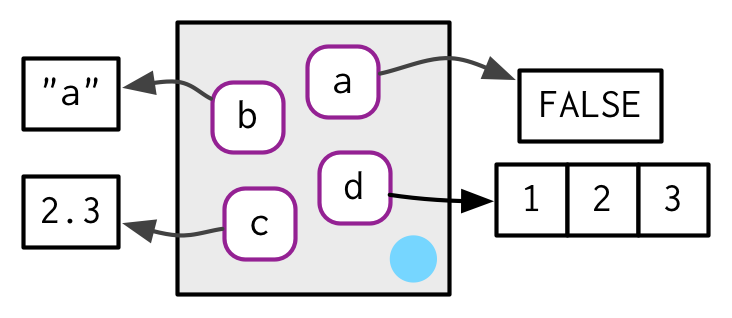
\includegraphics{diagrams/environments/bindings} \end{center}

就像在 \protect\hyperlink{env-modify}{names and values},
討論的,這個物件是參考為基礎.(in C concept) 不會有copy on
modifying。而且,環境物件可以自己指向自己(recursion)

\begin{Shaded}
\begin{Highlighting}[]
\NormalTok{e1}\OperatorTok{$}\NormalTok{d <-}\StringTok{ }\NormalTok{e1}
\end{Highlighting}
\end{Shaded}

\begin{center}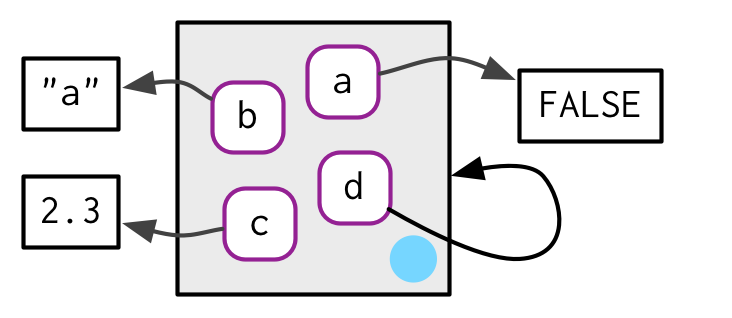
\includegraphics{diagrams/environments/loop} \end{center}

沒有指派的環境變數,只會顯示記憶體位址:

\begin{Shaded}
\begin{Highlighting}[]
\NormalTok{e1}
\end{Highlighting}
\end{Shaded}

要知道內容可以使用 \texttt{env\_print()} :

\begin{Shaded}
\begin{Highlighting}[]
\KeywordTok{env_print}\NormalTok{(e1)}
\end{Highlighting}
\end{Shaded}

想要知道目前有哪些binding(名稱-值 配對)可以利用 \texttt{env\_names()}

\begin{Shaded}
\begin{Highlighting}[]
\KeywordTok{env_names}\NormalTok{(e1)}
\end{Highlighting}
\end{Shaded}

::: base 要列出環境下的繫結,在R 3.2.0 以上,可以使用函數\texttt{names()}
,之前的版本則是 \texttt{ls()}, 但是要注意的是ls 的參數
\texttt{all.names} 內設是 \texttt{FALSE} 因此\texttt{.}開頭的看不到。.
:::

\subsection{Important environments}\label{important-environments}

另外參考 \protect\hyperlink{function-envs}{Special environments}。
\texttt{current\_env()}
可以知道目前程式碼的執行環境。例如,當我們互動執行RCODE的時候,環境通常是
\protect\hyperlink{globalux5cux2520environment}{總體環境},或者由函數\texttt{global\_env()}可以得到。這個總體環境有時候就叫``workspace'',同時,這也是函數外面所有互動計算發生的地方。
環境物件的比較不能用\texttt{==},只能用函數\texttt{identical()}。

\begin{Shaded}
\begin{Highlighting}[]
\KeywordTok{identical}\NormalTok{(}\KeywordTok{global_env}\NormalTok{(), }\KeywordTok{current_env}\NormalTok{())}
\end{Highlighting}
\end{Shaded}

\begin{Shaded}
\begin{Highlighting}[]
\KeywordTok{global_env}\NormalTok{() }\OperatorTok{==}\StringTok{ }\KeywordTok{current_env}\NormalTok{()}
\end{Highlighting}
\end{Shaded}

:::base

\begin{itemize}
\tightlist
\item
  \texttt{globalenv()} 和\texttt{.GlobalEnv}: 拿到global
  environmentand。
\item
  \texttt{environment()}:拿到目前的環境
\end{itemize}

global environment 的名稱為 \texttt{R\_GlobalEnv} 。

\begin{Shaded}
\begin{Highlighting}[]
\KeywordTok{global_env}\NormalTok{()}
\end{Highlighting}
\end{Shaded}

\begin{Shaded}
\begin{Highlighting}[]
\KeywordTok{current_env}\NormalTok{()}
\end{Highlighting}
\end{Shaded}

\begin{Shaded}
\begin{Highlighting}[]
\NormalTok{.GlobalEnv}
\end{Highlighting}
\end{Shaded}

:::

\subsection{Parents}\label{parents}

每一個環境物件都有一個\emph{parent}。\emph{parent}
也一個環境物件。在方塊圖中,parent以藍色圈表示,並用箭頭指向另一個環境物件。

這個parent用來建立 lexical scoping:
如果name沒有在某個環境物件找到,R會重複的在parent中找。
函數\texttt{env()}可以用來建立一個沒有名字的環境 You can set the parent
environment by supplying an unnamed argument to \texttt{env()}. If you
don't supply it, it defaults to the current environment.

\begin{Shaded}
\begin{Highlighting}[]
\NormalTok{e2a <-}\StringTok{ }\KeywordTok{env}\NormalTok{(}\DataTypeTok{d =} \DecValTok{4}\NormalTok{, }\DataTypeTok{e =} \DecValTok{5}\NormalTok{)}
\NormalTok{e2b <-}\StringTok{ }\KeywordTok{env}\NormalTok{(e2a, }\DataTypeTok{a =} \DecValTok{1}\NormalTok{, }\DataTypeTok{b =} \DecValTok{2}\NormalTok{, }\DataTypeTok{c =} \DecValTok{3}\NormalTok{)}
\end{Highlighting}
\end{Shaded}

\begin{center}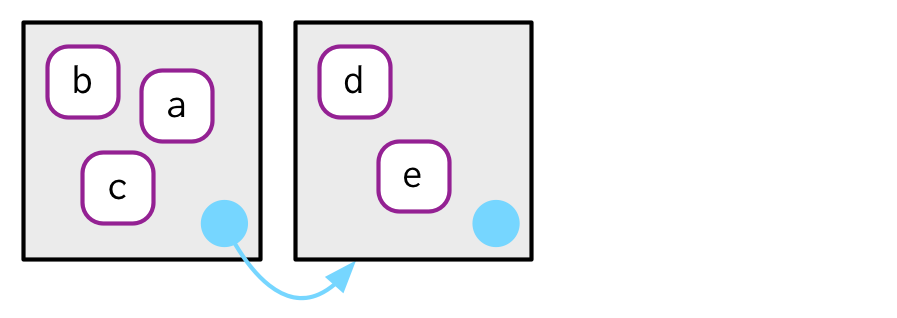
\includegraphics{diagrams/environments/parents} \end{center}

函數 \texttt{env\_parent()}可以用來找出某個環境物件的parent:

\begin{Shaded}
\begin{Highlighting}[]
\KeywordTok{env_parent}\NormalTok{(e2b)}
\end{Highlighting}
\end{Shaded}

\begin{Shaded}
\begin{Highlighting}[]
\KeywordTok{env_parent}\NormalTok{(e2a)}
\end{Highlighting}
\end{Shaded}

::: base parent.env() === env\_parent()

:::

所有的環境物件中只有一個名稱為\texttt{R\_EmptyEnv}的物件沒有parent(用空心藍色表示):

\begin{Shaded}
\begin{Highlighting}[]
\NormalTok{e2c <-}\StringTok{ }\KeywordTok{env}\NormalTok{(}\KeywordTok{empty_env}\NormalTok{(), }\DataTypeTok{d =} \DecValTok{4}\NormalTok{, }\DataTypeTok{e =} \DecValTok{5}\NormalTok{)}
\NormalTok{e2d <-}\StringTok{ }\KeywordTok{env}\NormalTok{(e2c, }\DataTypeTok{a =} \DecValTok{1}\NormalTok{, }\DataTypeTok{b =} \DecValTok{2}\NormalTok{, }\DataTypeTok{c =} \DecValTok{3}\NormalTok{)}
\end{Highlighting}
\end{Shaded}

\begin{center}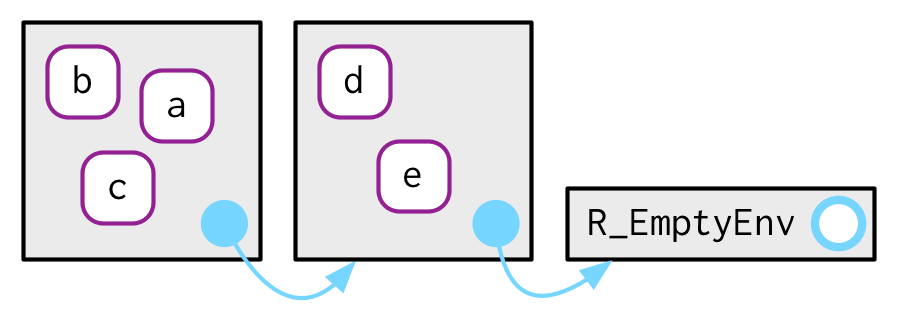
\includegraphics{diagrams/environments/parents-empty} \end{center}

::: base emptyenv() === empty\_env()

:::

試圖利用函數\texttt{env\_parent()}找空環境物件的parent會發生錯誤:

\begin{Shaded}
\begin{Highlighting}[]
\KeywordTok{env_parent}\NormalTok{(}\KeywordTok{empty_env}\NormalTok{())}
\end{Highlighting}
\end{Shaded}

函數
\texttt{env\_parents()}可以找出目前環境物件的所有祖先:這個函數會繼續直到遇上global
environment 或是空環境物件。上述過程可以利用\texttt{last}環境物件控制。

\begin{Shaded}
\begin{Highlighting}[]
\KeywordTok{env_parents}\NormalTok{(e2b)}
\end{Highlighting}
\end{Shaded}

\begin{Shaded}
\begin{Highlighting}[]
\KeywordTok{env_parents}\NormalTok{(e2d)}
\end{Highlighting}
\end{Shaded}

::: base 可以利用Use \texttt{parent.env()}
找到環境的parent,但是base中沒有可以找出所有祖先的函數。

:::

\subsection{Getting and setting}\label{getting-and-setting}

存取環境中元素的方法和list類似:使用 \texttt{\$} 和 \texttt{{[}{[}}:

\begin{Shaded}
\begin{Highlighting}[]
\NormalTok{e3 <-}\StringTok{ }\KeywordTok{env}\NormalTok{(}\DataTypeTok{x =} \DecValTok{1}\NormalTok{, }\DataTypeTok{y =} \DecValTok{2}\NormalTok{)}
\NormalTok{e3}\OperatorTok{$}\NormalTok{x}
\end{Highlighting}
\end{Shaded}

\begin{Shaded}
\begin{Highlighting}[]
\NormalTok{e3}\OperatorTok{$}\NormalTok{z <-}\StringTok{ }\DecValTok{3}
\NormalTok{e3[[}\StringTok{"z"}\NormalTok{]]}
\end{Highlighting}
\end{Shaded}

但是不能使用 \texttt{{[}{[}} +數字索引,也不能單獨使用 \texttt{{[}}:

\begin{Shaded}
\begin{Highlighting}[]
\NormalTok{e3[[}\DecValTok{1}\NormalTok{]]}
\end{Highlighting}
\end{Shaded}

\begin{Shaded}
\begin{Highlighting}[]
\NormalTok{e3[}\KeywordTok{c}\NormalTok{(}\StringTok{"x"}\NormalTok{, }\StringTok{"y"}\NormalTok{)]}
\end{Highlighting}
\end{Shaded}

當環境中的繫結不存在時(簡單點,就是變數不存在時)\texttt{\$} 和
\texttt{{[}{[}} 會傳回 \texttt{NULL}
但不會引發錯誤,如果要有錯誤警告,則利用 \texttt{env\_get()} :

\begin{Shaded}
\begin{Highlighting}[]
\NormalTok{e3}\OperatorTok{$}\NormalTok{xyz}
\end{Highlighting}
\end{Shaded}

\begin{Shaded}
\begin{Highlighting}[]
\KeywordTok{env_get}\NormalTok{(e3, }\StringTok{"xyz"}\NormalTok{)}
\end{Highlighting}
\end{Shaded}

當繫結不存在,但是想要有預設值傳回時,可以利用參數 \texttt{default} .

\begin{Shaded}
\begin{Highlighting}[]
\KeywordTok{env_get}\NormalTok{(e3, }\StringTok{"xyz"}\NormalTok{, }\DataTypeTok{default =} \OtherTok{NA}\NormalTok{)}
\end{Highlighting}
\end{Shaded}

另有兩種方式可以在環境物件加入繫結:

\begin{itemize}
\item
  \texttt{env\_poke()}\footnote{You might wonder why rlang has
    \texttt{env\_poke()} instead of \texttt{env\_set()}. This is for
    consistency: \texttt{\_set()} functions return a modified copy;
    \texttt{\_poke()} functions modify in place.} takes a name (as
  string) and a value:

\begin{Shaded}
\begin{Highlighting}[]
\KeywordTok{env_poke}\NormalTok{(e3, }\StringTok{"a"}\NormalTok{, }\DecValTok{100}\NormalTok{)}
\NormalTok{e3}\OperatorTok{$}\NormalTok{a}
\end{Highlighting}
\end{Shaded}
\item
  \texttt{env\_bind()} allows you to bind multiple values:

\begin{Shaded}
\begin{Highlighting}[]
\KeywordTok{env_bind}\NormalTok{(e3, }\DataTypeTok{a =} \DecValTok{10}\NormalTok{, }\DataTypeTok{b =} \DecValTok{20}\NormalTok{)}
\KeywordTok{env_names}\NormalTok{(e3)}
\end{Highlighting}
\end{Shaded}
\end{itemize}

\texttt{env\_has()}: 是否環境中有繫結

\begin{Shaded}
\begin{Highlighting}[]
\KeywordTok{env_has}\NormalTok{(e3, }\StringTok{"a"}\NormalTok{)}
\end{Highlighting}
\end{Shaded}

不能像是list中刪除元素的方式(指派\texttt{NULL}給元素),而必須使用
\texttt{env\_unbind()}:

\begin{Shaded}
\begin{Highlighting}[]
\NormalTok{e3}\OperatorTok{$}\NormalTok{a <-}\StringTok{ }\OtherTok{NULL}
\KeywordTok{env_has}\NormalTok{(e3, }\StringTok{"a"}\NormalTok{)}
\end{Highlighting}
\end{Shaded}

\begin{Shaded}
\begin{Highlighting}[]
\KeywordTok{env_unbind}\NormalTok{(e3, }\StringTok{"a"}\NormalTok{)}
\KeywordTok{env_has}\NormalTok{(e3, }\StringTok{"a"}\NormalTok{)}
\end{Highlighting}
\end{Shaded}

從一個物件Unbinding 解除名稱,並不會刪除物件,是否刪除物件是 garbage
collector的工作.。可以參考 \protect\hyperlink{gc}{GC}.

::: base

See \texttt{get()}, \texttt{assign()}, \texttt{exists()}, and
\texttt{rm()}. These are designed interactively for use with the current
environment, so working with other environments is a little clunky. Also
beware the \texttt{inherits} argument: it defaults to \texttt{TRUE}
meaning that the base equivalents will inspect the supplied environment
and all its ancestors. :::

\subsection{Finalisers}\label{finalisers}

{Add something once rlang has an API. Also mention in data structures
below}

\hypertarget{advanced-bindings}{\subsection{Advanced
bindings}\label{advanced-bindings}}

There are two more exotic variants of \texttt{env\_bind()}:

\begin{itemize}
\item
  \texttt{env\_bind\_exprs()} creates \textbf{delayed bindings}, which
  are evaluated the first time they are accessed. Behind the scenes,
  delayed bindings create promises, so behave in the same way as
  function arguments.

\begin{Shaded}
\begin{Highlighting}[]
\KeywordTok{env_bind_exprs}\NormalTok{(}\KeywordTok{current_env}\NormalTok{(), }\DataTypeTok{b =}\NormalTok{ \{}\KeywordTok{Sys.sleep}\NormalTok{(}\DecValTok{1}\NormalTok{); }\DecValTok{1}\NormalTok{\})}
\end{Highlighting}
\end{Shaded}

\begin{Shaded}
\begin{Highlighting}[]
\KeywordTok{system.time}\NormalTok{(}\KeywordTok{print}\NormalTok{(b))}
\end{Highlighting}
\end{Shaded}

\begin{Shaded}
\begin{Highlighting}[]
\KeywordTok{system.time}\NormalTok{(}\KeywordTok{print}\NormalTok{(b))}
\end{Highlighting}
\end{Shaded}

  Delayed bindings are used to implement \texttt{autoload()}, which
  makes R behave as if the package data is in memory, even though it's
  only loaded from disk when you ask for it.
\item
  \texttt{env\_bind\_fns()} creates \textbf{active bindings} which are
  re-computed every time they're accessed:

\begin{Shaded}
\begin{Highlighting}[]
\KeywordTok{env_bind_fns}\NormalTok{(}\KeywordTok{current_env}\NormalTok{(), }\DataTypeTok{z1 =} \ControlFlowTok{function}\NormalTok{(val) }\KeywordTok{runif}\NormalTok{(}\DecValTok{1}\NormalTok{))}
\end{Highlighting}
\end{Shaded}

\begin{Shaded}
\begin{Highlighting}[]
\NormalTok{z1}
\end{Highlighting}
\end{Shaded}

\begin{Shaded}
\begin{Highlighting}[]
\NormalTok{z1}
\end{Highlighting}
\end{Shaded}

  The argument to the function allows you to also override behaviour
  when the variable is set:

\begin{Shaded}
\begin{Highlighting}[]
\KeywordTok{env_bind_fns}\NormalTok{(}\KeywordTok{current_env}\NormalTok{(), }\DataTypeTok{z2 =} \ControlFlowTok{function}\NormalTok{(val) \{}
  \ControlFlowTok{if}\NormalTok{ (}\KeywordTok{missing}\NormalTok{(val)) \{}
    \DecValTok{2}
\NormalTok{  \} }\ControlFlowTok{else}\NormalTok{ \{}
     \KeywordTok{stop}\NormalTok{(}\StringTok{"Don't touch z2!"}\NormalTok{, }\DataTypeTok{call. =} \OtherTok{FALSE}\NormalTok{)}
\NormalTok{  \}}
\NormalTok{\})}

\NormalTok{z2}
\end{Highlighting}
\end{Shaded}

\begin{Shaded}
\begin{Highlighting}[]
\NormalTok{z2 <-}\StringTok{ }\DecValTok{3}
\end{Highlighting}
\end{Shaded}
\end{itemize}

::: base See \texttt{?delayedAssign()} and
\texttt{?makeActiveBinding()}. :::

\subsection{Exercises}\label{exercises-6}

\begin{enumerate}
\def\labelenumi{\arabic{enumi}.}
\item
  List three ways in which an environment differs from a list.
\item
  Create an environment as illustrated by this picture.

  \begin{center}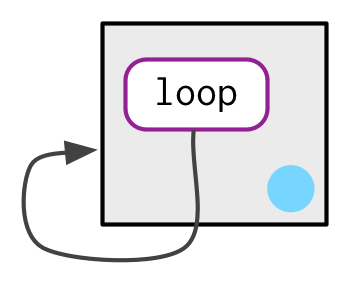
\includegraphics{diagrams/environments/recursive-1} \end{center}
\item
  Create a pair of environments as illustrated by this picture.

  \begin{center}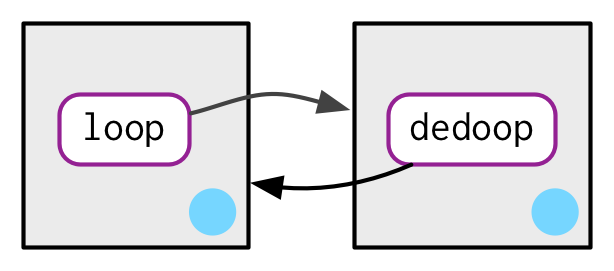
\includegraphics{diagrams/environments/recursive-2} \end{center}
\item
  Explain why \texttt{e{[}{[}1{]}{]}} and \texttt{e{[}c("a",\ "b"){]}}
  don't make sense when \texttt{e} is an environment.
\item
  Create a version of \texttt{env\_poke()} that will only bind new
  names, never re-bind old names. Some programming languages only do
  this, and are known as
  \href{http://en.wikipedia.org/wiki/Assignment_(computer_science)\#Single_assignment}{single
  assignment languages}.
\end{enumerate}

\hypertarget{env-recursion}{\section{Recursing over
environments}\label{env-recursion}}

If you want to operate on every ancestor of an environment, it's often
convenient to write a recursive function. This section shows you how,
applying your new knowledge of environments to write a function that
given a name, finds the environment \texttt{where()} that name is
defined, using R's regular scoping rules.

The definition of \texttt{where()} is straightforward. It has two
arguments: the name to look for (as a string), and the environment in
which to start the search. (We'll learn why \texttt{caller\_env()} is a
good default in \protect\hyperlink{calling-environments}{calling
environments}.)

\begin{Shaded}
\begin{Highlighting}[]
\NormalTok{where <-}\StringTok{ }\ControlFlowTok{function}\NormalTok{(name, }\DataTypeTok{env =} \KeywordTok{caller_env}\NormalTok{()) \{}
  \ControlFlowTok{if}\NormalTok{ (}\KeywordTok{identical}\NormalTok{(env, }\KeywordTok{empty_env}\NormalTok{())) \{}
    \CommentTok{# Base case}
    \KeywordTok{stop}\NormalTok{(}\StringTok{"Can't find "}\NormalTok{, name, }\DataTypeTok{call. =} \OtherTok{FALSE}\NormalTok{)}
\NormalTok{  \} }\ControlFlowTok{else} \ControlFlowTok{if}\NormalTok{ (}\KeywordTok{env_has}\NormalTok{(env, name)) \{}
    \CommentTok{# Success case}
\NormalTok{    env}
\NormalTok{  \} }\ControlFlowTok{else}\NormalTok{ \{}
    \CommentTok{# Recursive case}
    \KeywordTok{where}\NormalTok{(name, }\KeywordTok{env_parent}\NormalTok{(env))}
\NormalTok{  \}}
\NormalTok{\}}
\end{Highlighting}
\end{Shaded}

3個情況:

\begin{itemize}
\item
  The base case: 到達empty environment 沒有parent無法繼續,所以丟出error.
\item
  The successful case: 在env中找到name ,成功,所以傳回env。.
\item
  The recursive case: 在env中找不到,繼續在parent中找。.
\end{itemize}

These three cases are illustrated with these three examples:

\begin{Shaded}
\begin{Highlighting}[]
\KeywordTok{where}\NormalTok{(}\StringTok{"yyy"}\NormalTok{)}
\end{Highlighting}
\end{Shaded}

\begin{Shaded}
\begin{Highlighting}[]
\NormalTok{x <-}\StringTok{ }\DecValTok{5}
\KeywordTok{where}\NormalTok{(}\StringTok{"x"}\NormalTok{)}
\end{Highlighting}
\end{Shaded}

\begin{Shaded}
\begin{Highlighting}[]
\KeywordTok{where}\NormalTok{(}\StringTok{"mean"}\NormalTok{)}
\end{Highlighting}
\end{Shaded}

想像有兩個環境物件(如圖):

\begin{Shaded}
\begin{Highlighting}[]
\NormalTok{e4a <-}\StringTok{ }\KeywordTok{env}\NormalTok{(}\KeywordTok{empty_env}\NormalTok{(), }\DataTypeTok{a =} \DecValTok{1}\NormalTok{, }\DataTypeTok{b =} \DecValTok{2}\NormalTok{)}
\NormalTok{e4b <-}\StringTok{ }\KeywordTok{env}\NormalTok{(e4a, }\DataTypeTok{x =} \DecValTok{10}\NormalTok{, }\DataTypeTok{a =} \DecValTok{11}\NormalTok{)}
\end{Highlighting}
\end{Shaded}

\begin{center}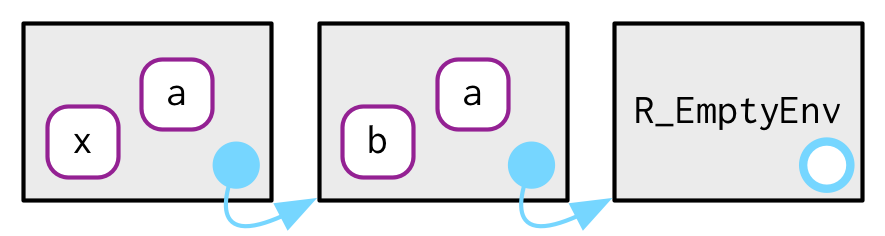
\includegraphics{diagrams/environments/where-ex} \end{center}

\begin{itemize}
\item
  \texttt{where(a,\ e4a)} will find \texttt{a} in \texttt{e4a}.
\item
  \texttt{where("b",\ e4a)} doesn't find \texttt{b} in \texttt{e4a}, so
  it looks in its parent, \texttt{e4b}, and finds it there.
\item
  \texttt{where("c",\ e4a)} looks in \texttt{e4a}, then \texttt{e4b},
  then hits the empty environment and throws an error.
\end{itemize}

It's natural to work with environments recursively, so \texttt{where()}
provides a useful template. Removing the specifics of \texttt{where()}
shows the structure more clearly:

\begin{Shaded}
\begin{Highlighting}[]
\NormalTok{f <-}\StringTok{ }\ControlFlowTok{function}\NormalTok{(..., }\DataTypeTok{env =} \KeywordTok{caller_env}\NormalTok{()) \{}
  \ControlFlowTok{if}\NormalTok{ (}\KeywordTok{identical}\NormalTok{(env, }\KeywordTok{empty_env}\NormalTok{())) \{}
    \CommentTok{# base case}
\NormalTok{  \} }\ControlFlowTok{else} \ControlFlowTok{if}\NormalTok{ (success) \{}
    \CommentTok{# success case}
\NormalTok{  \} }\ControlFlowTok{else}\NormalTok{ \{}
    \CommentTok{# recursive case}
    \KeywordTok{f}\NormalTok{(..., }\DataTypeTok{env =} \KeywordTok{env_parent}\NormalTok{(env))}
\NormalTok{  \}}
\NormalTok{\}}
\end{Highlighting}
\end{Shaded}

::: sidebar \#\#\# Iteration vs recursion \{-\}

也可以用迭代的方式

\begin{Shaded}
\begin{Highlighting}[]
\NormalTok{f2 <-}\StringTok{ }\ControlFlowTok{function}\NormalTok{(..., }\DataTypeTok{env =} \KeywordTok{caller_env}\NormalTok{()) \{}
  \ControlFlowTok{while}\NormalTok{ (}\OperatorTok{!}\KeywordTok{identical}\NormalTok{(env, }\KeywordTok{empty_env}\NormalTok{())) \{}
    \ControlFlowTok{if}\NormalTok{ (success) \{}
      \CommentTok{# success case}
      \KeywordTok{return}\NormalTok{()}
\NormalTok{    \}}
    \CommentTok{# inspect parent}
\NormalTok{    env <-}\StringTok{ }\KeywordTok{env_parent}\NormalTok{(env)}
\NormalTok{  \}}

  \CommentTok{# base case}
\NormalTok{\}}
\end{Highlighting}
\end{Shaded}

:::

\subsection{Exercises}\label{exercises-7}

\begin{enumerate}
\def\labelenumi{\arabic{enumi}.}
\item
  Modify \texttt{where()} to return \emph{all} environments that contain
  a binding for \texttt{name}. Carefully think through what type of
  object the function will need to return.
\item
  Write a function called \texttt{fget()} that finds only function
  objects. It should have two arguments, \texttt{name} and \texttt{env},
  and should obey the regular scoping rules for functions: if there's an
  object with a matching name that's not a function, look in the parent.
  For an added challenge, also add an \texttt{inherits} argument which
  controls whether the function recurses up the parents or only looks in
  one environment.
\end{enumerate}

\hypertarget{function-envs}{\section{Special
environments}\label{function-envs}}

這裡討論 package environments.
然後探討當函數建立時,綁入函數的函數環境。還有當函數被呼叫時的執行環境(ephemeral)。

\href{package-environments}{套裝環境}主要是看這些環境如何支援namespaces。同時,namespace讓package每次載入的時候,都有一樣的行為,而不售其他packages載入先後的影響。

\subsection{Package environments and the search
path}\label{package-environments-and-the-search-path}

每個套件經由\texttt{library()} 或 \texttt{require()}
接入成為\protect\hyperlink{global-environment}{總體環境}的parent。而最後一個\protect\hyperlink{attach}{接入}的套件,則是總體環境的第一個parent:

::: sidebar load 和
attach不一樣,當我們使用library的時候,我們做的是{[}\^{}attach{]}
在環境串列中加入我們利用library載入的物件.. {[}\^{}attach{]}: Note the
difference between attached and loaded. A package is loaded
automatically if you access one of its functions using \texttt{::}; it
is only \textbf{attached} to the search path by \texttt{library()} or
\texttt{require()}.

:::

\begin{Shaded}
\begin{Highlighting}[]
\KeywordTok{env_parent}\NormalTok{(}\KeywordTok{global_env}\NormalTok{())}
\end{Highlighting}
\end{Shaded}

And the parent of that package is the second to last package you
attached:

\begin{Shaded}
\begin{Highlighting}[]
\KeywordTok{env_parent}\NormalTok{(}\KeywordTok{env_parent}\NormalTok{(}\KeywordTok{global_env}\NormalTok{()))}
\end{Highlighting}
\end{Shaded}

如果一層一層parent回朔,就可以到每個套件被接入的順序,這也是R執行中會用到的
\textbf{search path} 因為這些環境的所有物件都可以經由 top-level
interactive workspace找到。

\begin{Shaded}
\begin{Highlighting}[]
\KeywordTok{search_envs}\NormalTok{()}
\end{Highlighting}
\end{Shaded}

:::base 函數 \texttt{search()}可以找出環境物件的名稱。 :::

最後兩個環境物件都一樣:

\begin{itemize}
\item
  \texttt{Autoloads} 環境物件,利用 delayed
  bindings來節省記憶體,也就是在需要的時候才載入(loading)package中的物件(例如大型資料集)。
\item
  base environment, \texttt{package:base} 或簡稱 \texttt{base}, 是base
  套裝的環境物件。用來 載入其他套裝(bootstrap)。利用函數
  \texttt{base\_env()}存取.
\end{itemize}

利用圖型表示:

\begin{center}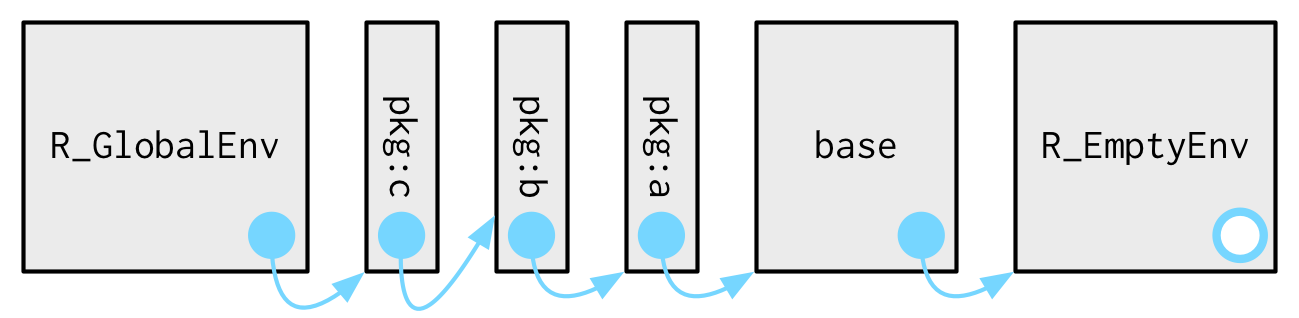
\includegraphics{diagrams/environments/search-path} \end{center}

當利用 \texttt{library()} attach其他套件的時候,
總體環境的parent馬上改變:

\begin{center}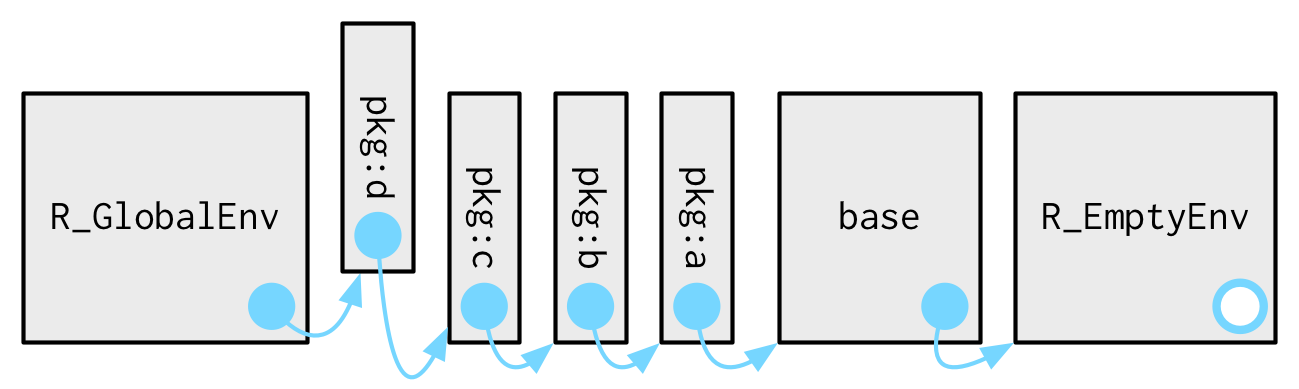
\includegraphics{diagrams/environments/search-path-2} \end{center}

\subsection{The function environment}\label{the-function-environment}

當函數被建立的時候,現有的環境會被繫結。稱為\emph{function environment},
主要用來支援lexical scoping.
在電腦語言中,當函數紀錄它們的運作環境時,我們說這個函數屬於
\emph{closures}。,這也是為甚麼這個字眼經常在R語言中出現。.

利用函數 \texttt{fn\_env()}可以得到函數的環境物件:

\begin{Shaded}
\begin{Highlighting}[]
\NormalTok{y <-}\StringTok{ }\DecValTok{1}
\NormalTok{f <-}\StringTok{ }\ControlFlowTok{function}\NormalTok{(x) x }\OperatorTok{+}\StringTok{ }\NormalTok{y}
\KeywordTok{fn_env}\NormalTok{(f)}
\end{Highlighting}
\end{Shaded}

::: base 一樣利用函數 \texttt{environment(f)} 可以找到函數
\texttt{f}的環境. :::

在圖形中,函數被畫成類似子彈,而彈頭的部分繫結環境。

\begin{center}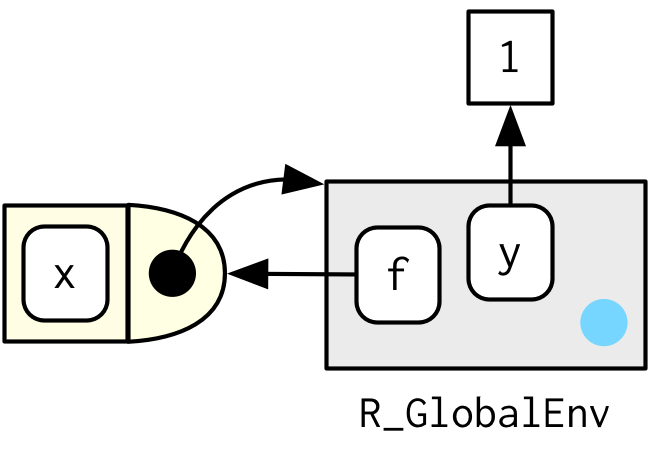
\includegraphics{diagrams/environments/binding} \end{center}

在這個案例中,\texttt{f()}繫結的環境物件,就是繫結名稱\texttt{f}的環境。但並不一定總是這樣,例如在下一個例子中,\texttt{g}被繫結在新環境物件\texttt{e}中。但是函數\texttt{g()}繫結的是global
environment。這之間的分別是我們如何找到\texttt{g}和\texttt{g}如何找到他的變數。

\begin{Shaded}
\begin{Highlighting}[]
\NormalTok{e <-}\StringTok{ }\KeywordTok{env}\NormalTok{()}
\NormalTok{e}\OperatorTok{$}\NormalTok{g <-}\StringTok{ }\ControlFlowTok{function}\NormalTok{() }\DecValTok{1}
\end{Highlighting}
\end{Shaded}

\begin{center}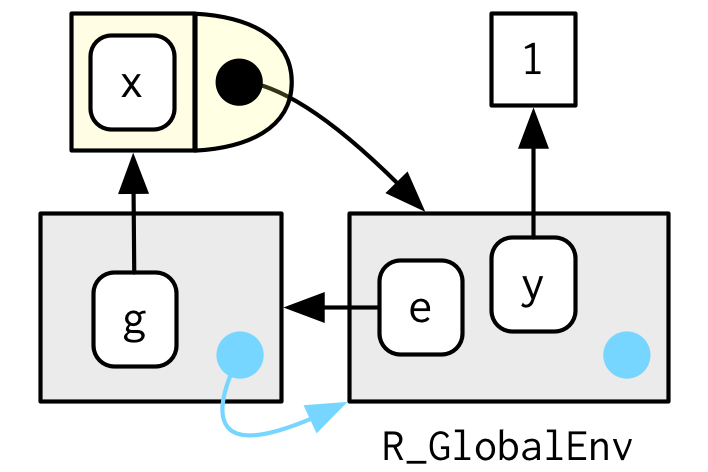
\includegraphics{diagrams/environments/binding-2} \end{center}

\subsection{Namespaces}\label{namespaces}

在上面的圖形中,我們已經知道套件的parent會隨著之前套件載入的順序不同而不同。這就導致R程式設計者必須保證個別套件上如果使用別的套件的函數,必須是原始目的的那一個。\emph{namespaces}
就是為此目的而產生: 每個套件必須的使用必須一致,而不管使用者如何載入套件.

以 \texttt{sd()}為例子:

\begin{Shaded}
\begin{Highlighting}[]
\NormalTok{sd}
\end{Highlighting}
\end{Shaded}

\texttt{sd()} 必須使用函數 \texttt{var()},
因此這個\texttt{var()}到底來自 global
environment,還是其他接入(attached)的套件的這種問題必須避免。 R avoids
this problem by taking advantage of the function vs.~binding environment
described above.

每個套件中的函數和一對環境物件有關:套件環境(之前學到的)還有\emph{namespace}環境物件。

\begin{itemize}
\item
  package environment:
  是套件的外部介面,這是R使用者如何在接入的套件中尋找函數的地方(或者可以利用
  \texttt{::}) package enviromnent 的parent
  由搜尋路徑決定(可以利用\texttt{search()}知道)決定(也就是載入的順序)
\item
  namespace environment:是套件的內部介面。package environment
  控制我們如何找到函數,而namespace environment控制函數如何找到變數。
\end{itemize}

在package environment的每個繫結也可以在namespace
environment中找到。這樣可以確保每個函數可以使用套件中的其他函數。但是有些繫結只能在namespace
中找到(例如內部或非輸出物件),這種內部物件通常是用來隱藏一些繁瑣的且不需要給使用者看到的細節。;

\begin{center}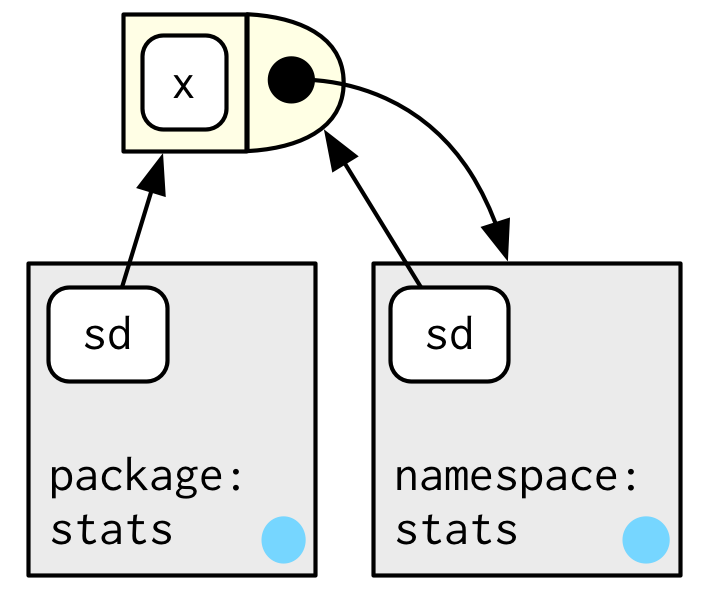
\includegraphics{diagrams/environments/namespace-bind} \end{center}

每個namespace environment 有一樣的祖集合:

\begin{itemize}
\item
  每個namespace有\emph{imports}的環境物件,其中包含了套件中用到的所有函數繫結。而所謂\protect\hyperlink{imports-environment}{輸入環境}實際由套裝開發人員在檔案\texttt{NAMESPACE}指定
\item
  明確的輸入每個\texttt{base}函數,很繁瑣,所以R直接設定\texttt{import\ enviroment}的parent是\texttt{base\ *namespae*}{[}\^{}1{]}。
\end{itemize}

::: sidebar The base namespace contains the same bindings as the base
environment, but it has different parent. :::

\begin{itemize}
\tightlist
\item
  \emph{base namespace} 的parent是總體環境(\#global
  environment).參考下圖,這種設計導致在import
  environment中找不到繫結時,會開始再總體環境中尋找,而之前提過總體環境通常是互動環境下名稱搜尋的開始路徑,這也導致搜尋的方式受到套件載入順序的影響。因此,R提供了了\texttt{R\ CMD\ check}來警告此種情況的發生。(雖然有麻煩,但是由於S3
  方法的dispatch 關係,此種方式仍然留著)
\end{itemize}

\begin{center}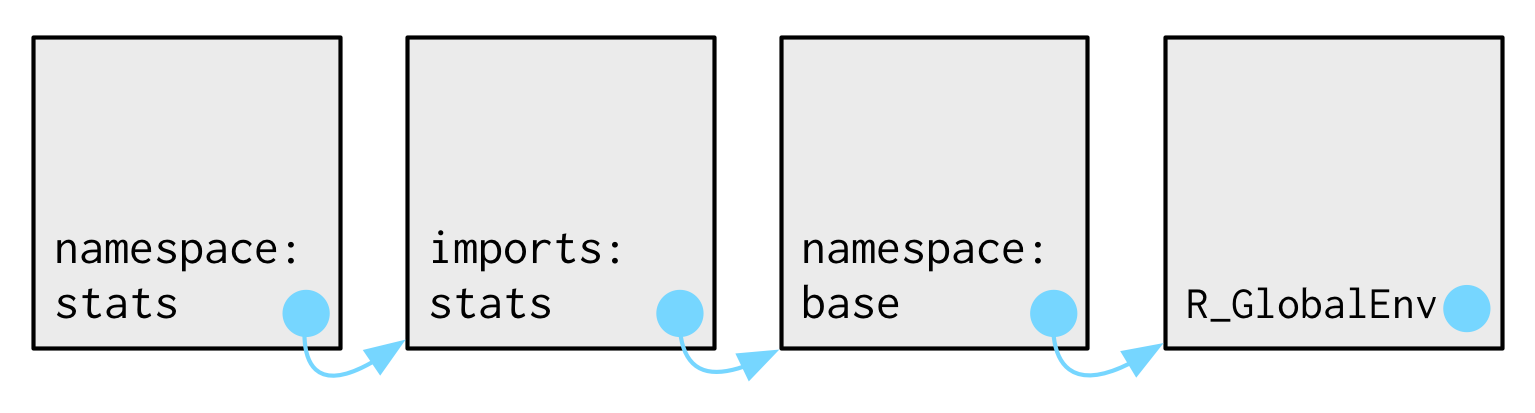
\includegraphics{diagrams/environments/namespace-env} \end{center}

綜合上述,可以得到下圖::

\begin{center}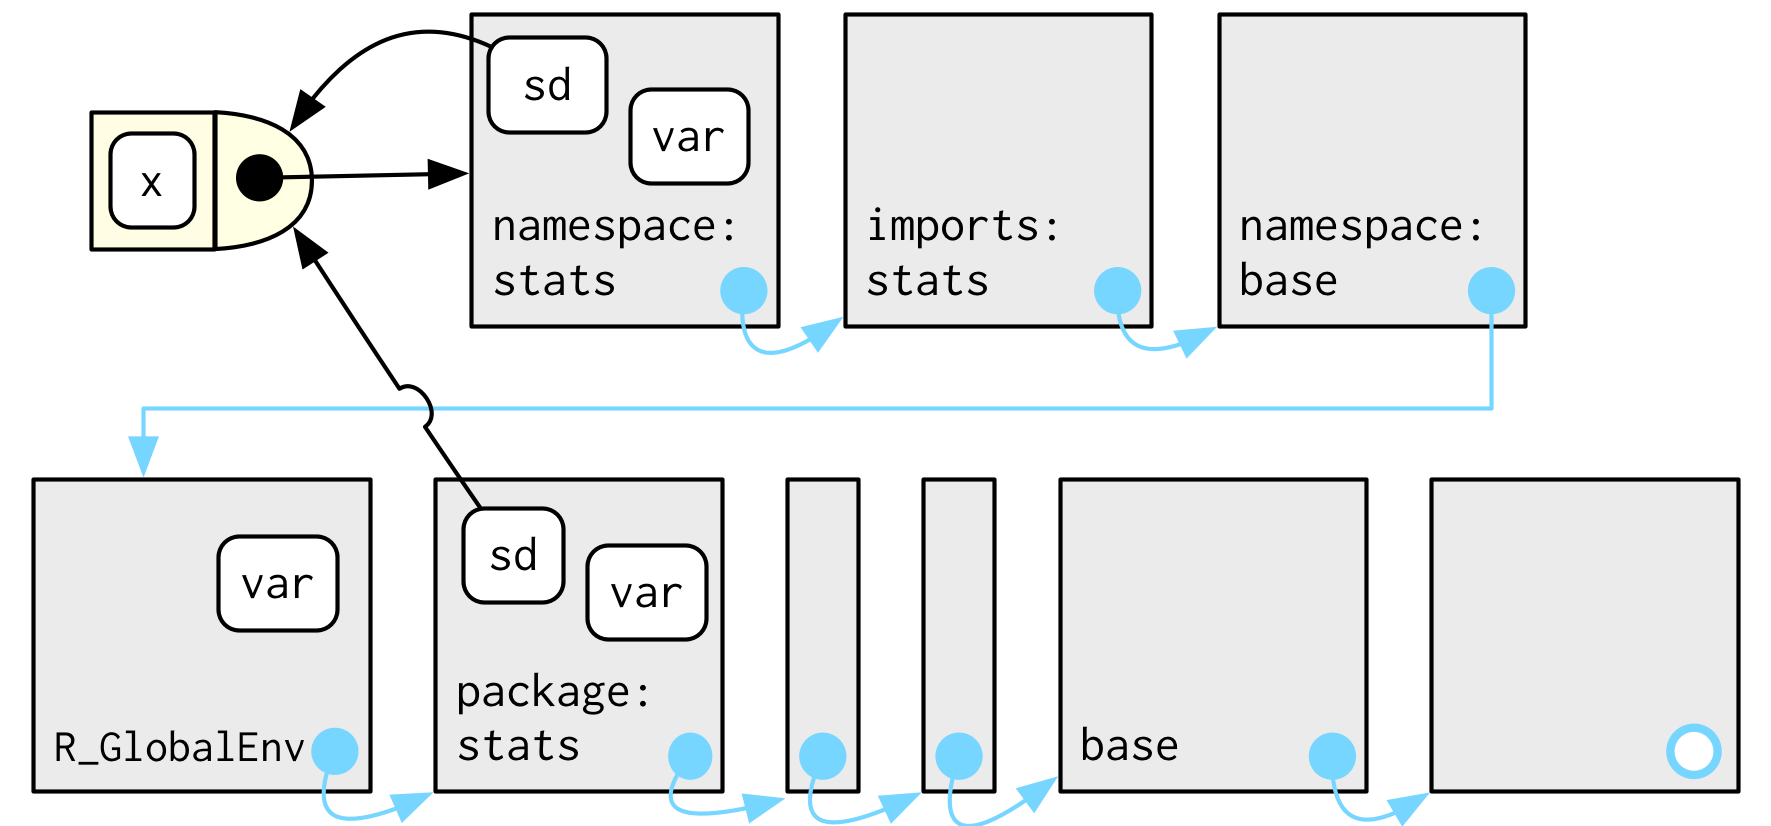
\includegraphics{diagrams/environments/namespace} \end{center}

所以當 \texttt{sd()} 搜尋\texttt{var}
的值的時候,搜尋順序是受到開發者的指定(在檔案NAMESPACE利用import),而不會受到套裝使用者的影響。這樣保證每次套件程式碼執行的時候,都一樣,而不會受到一般使用者載入套件的順序而影響。

注意在package和namespace兩種環境之間沒有直接的連結.連結是由\emph{函數環境}定義。

\subsection{Execution environments}\label{execution-environments}

\textbf{execution} environment.
下面的函數第一次執行的時候會傳回甚麼?第2次呢?

\begin{Shaded}
\begin{Highlighting}[]
\NormalTok{g <-}\StringTok{ }\ControlFlowTok{function}\NormalTok{(x) \{}
  \ControlFlowTok{if}\NormalTok{ (}\OperatorTok{!}\KeywordTok{env_has}\NormalTok{(}\KeywordTok{current_env}\NormalTok{(), }\StringTok{"a"}\NormalTok{)) \{}
    \KeywordTok{message}\NormalTok{(}\StringTok{"Defining a"}\NormalTok{)}
\NormalTok{    a <-}\StringTok{ }\DecValTok{1}
\NormalTok{  \} }\ControlFlowTok{else}\NormalTok{ \{}
\NormalTok{    a <-}\StringTok{ }\NormalTok{a }\OperatorTok{+}\StringTok{ }\DecValTok{1}
\NormalTok{  \}}
\NormalTok{  a}
\NormalTok{\}}
\end{Highlighting}
\end{Shaded}

再一次利用下面的調用,確認你的答案:

\begin{Shaded}
\begin{Highlighting}[]
\KeywordTok{g}\NormalTok{(}\DecValTok{10}\NormalTok{)}
\end{Highlighting}
\end{Shaded}

\begin{verbatim}
Defining a
\end{verbatim}

\begin{Shaded}
\begin{Highlighting}[]
\KeywordTok{g}\NormalTok{(}\DecValTok{10}\NormalTok{)}
\end{Highlighting}
\end{Shaded}

\begin{verbatim}
Defining a
\end{verbatim}

\begin{Shaded}
\begin{Highlighting}[]
\KeywordTok{g}\NormalTok{(}\DecValTok{11}\NormalTok{)}
\end{Highlighting}
\end{Shaded}

\begin{verbatim}
Defining a
\end{verbatim}

這個函數每次執行都傳回一樣的答案,參考 \protect\hyperlink{fresh-start}{a
fresh start}.
每次函數被調用的時候,一個新的環境都會被建立來主導執行。這種環境稱為\emph{執行環境}。而\emph{執行環境}的parent為
function environment.

用另一個簡單點的例子說明. (圖中,執行環境的parent間接表示:經由函數環境).

\begin{Shaded}
\begin{Highlighting}[]
\NormalTok{h <-}\StringTok{ }\ControlFlowTok{function}\NormalTok{(x) \{}
  \CommentTok{# 1.}
\NormalTok{  a <-}\StringTok{ }\DecValTok{2} \CommentTok{# 2.}
\NormalTok{  x }\OperatorTok{+}\StringTok{ }\NormalTok{a}
\NormalTok{\}}
\NormalTok{y <-}\StringTok{ }\KeywordTok{h}\NormalTok{(}\DecValTok{1}\NormalTok{) }\CommentTok{# 3.}
\end{Highlighting}
\end{Shaded}

\begin{center}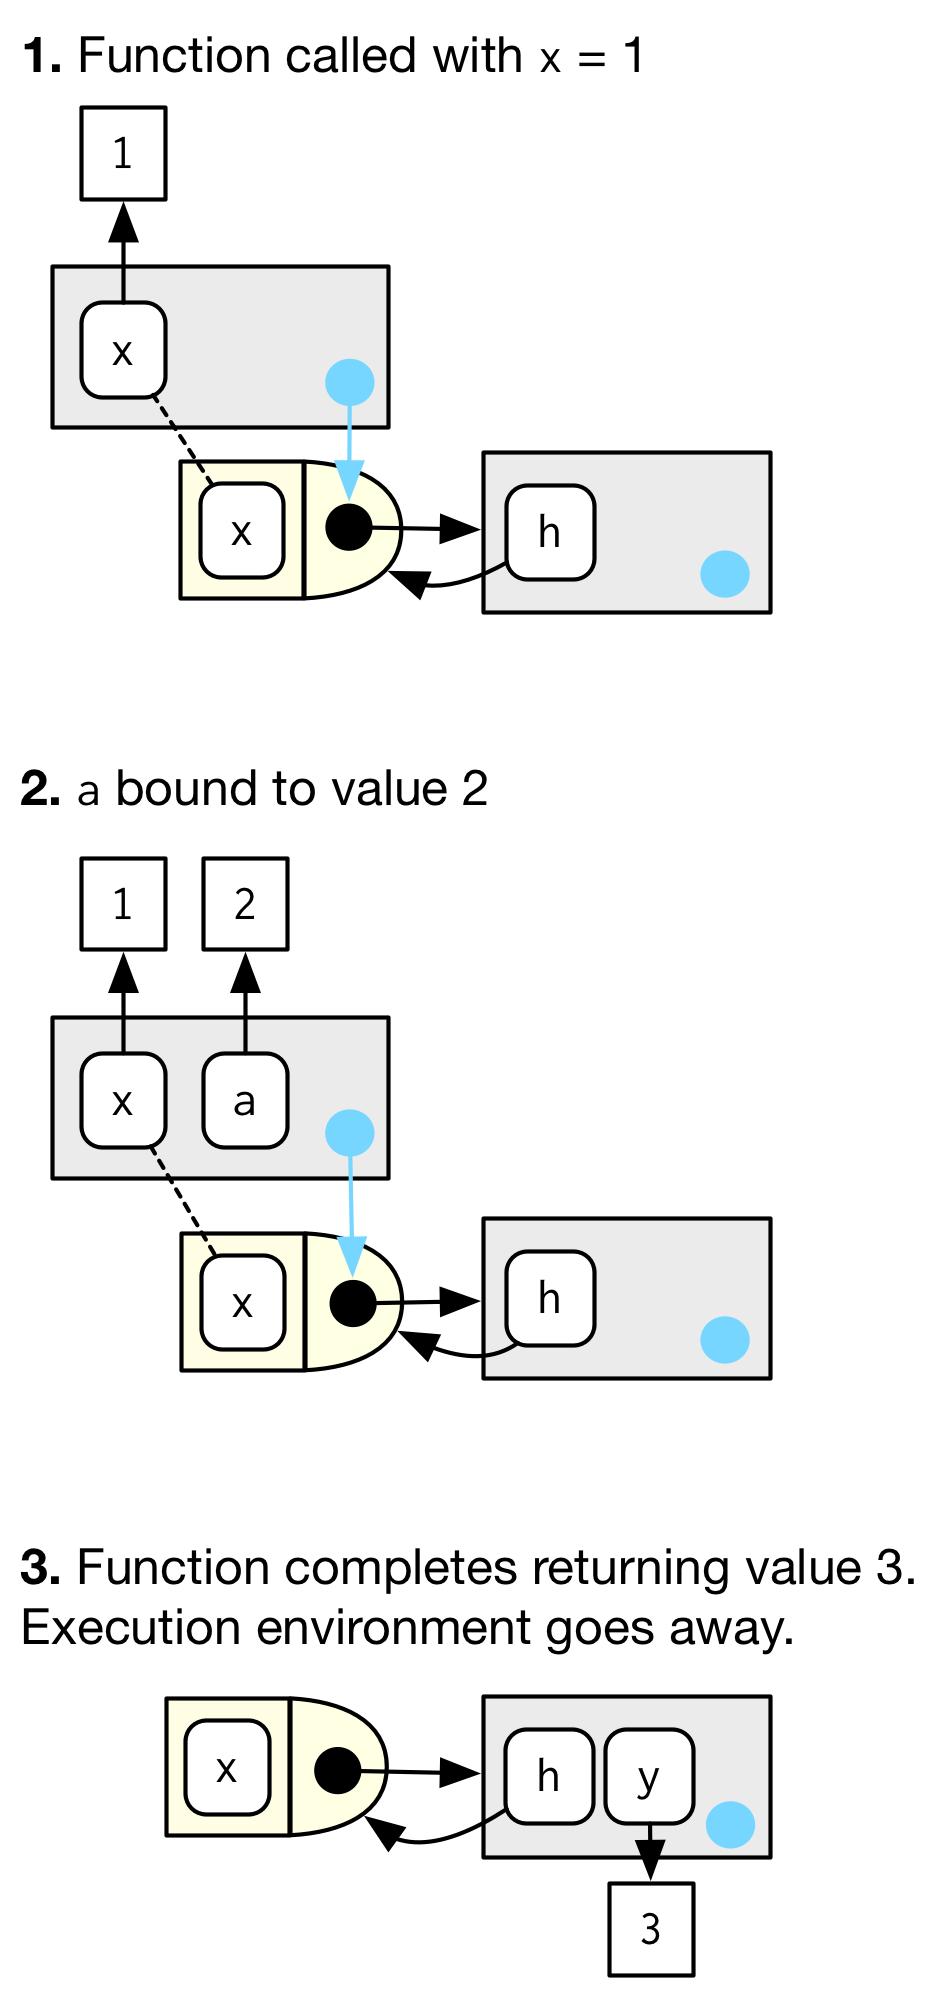
\includegraphics{diagrams/environments/execution} \end{center}

執行環境(execution
environment)短暫存在,當函數執行完畢通常會被GC。在幾種情況下,會在記憶體存在比較久,第一種是回傳給另一個變數:

\begin{Shaded}
\begin{Highlighting}[]
\NormalTok{h2 <-}\StringTok{ }\ControlFlowTok{function}\NormalTok{(x) \{}
\NormalTok{  a <-}\StringTok{ }\NormalTok{x }\OperatorTok{*}\StringTok{ }\DecValTok{2}
  \KeywordTok{current_env}\NormalTok{()}
\NormalTok{\}}

\NormalTok{e <-}\StringTok{ }\KeywordTok{h2}\NormalTok{(}\DataTypeTok{x =} \DecValTok{10}\NormalTok{)}
\KeywordTok{env_print}\NormalTok{(e)}
\end{Highlighting}
\end{Shaded}

\begin{Shaded}
\begin{Highlighting}[]
\KeywordTok{fn_env}\NormalTok{(h2)}
\end{Highlighting}
\end{Shaded}

Another way to capture it is to return an object with a binding to that
environment, like a function. The following example illustrates that
idea with a function factory, \texttt{plus()}. We use that factory to
create a function called \texttt{plus\_one()}.

There's a lot going on in the diagram because the enclosing environment
of \texttt{plus\_one()} is the execution environment of \texttt{plus()}.

\begin{Shaded}
\begin{Highlighting}[]
\NormalTok{plus <-}\StringTok{ }\ControlFlowTok{function}\NormalTok{(x) \{}
  \ControlFlowTok{function}\NormalTok{(y) x }\OperatorTok{+}\StringTok{ }\NormalTok{y}
\NormalTok{\}}

\NormalTok{plus_one <-}\StringTok{ }\KeywordTok{plus}\NormalTok{(}\DecValTok{1}\NormalTok{)}
\NormalTok{plus_one}
\end{Highlighting}
\end{Shaded}

\begin{center}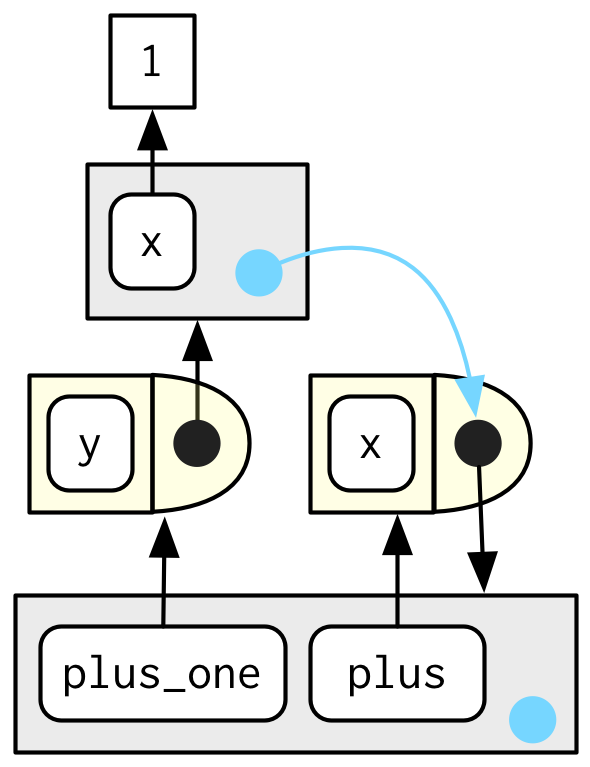
\includegraphics{diagrams/environments/closure} \end{center}

What happens when we call \texttt{plus\_one()}? Its execution
environment will have the captured execution environment of
\texttt{plus()} as its parent:

\begin{Shaded}
\begin{Highlighting}[]
\KeywordTok{plus_one}\NormalTok{(}\DecValTok{2}\NormalTok{)}
\end{Highlighting}
\end{Shaded}

\begin{center}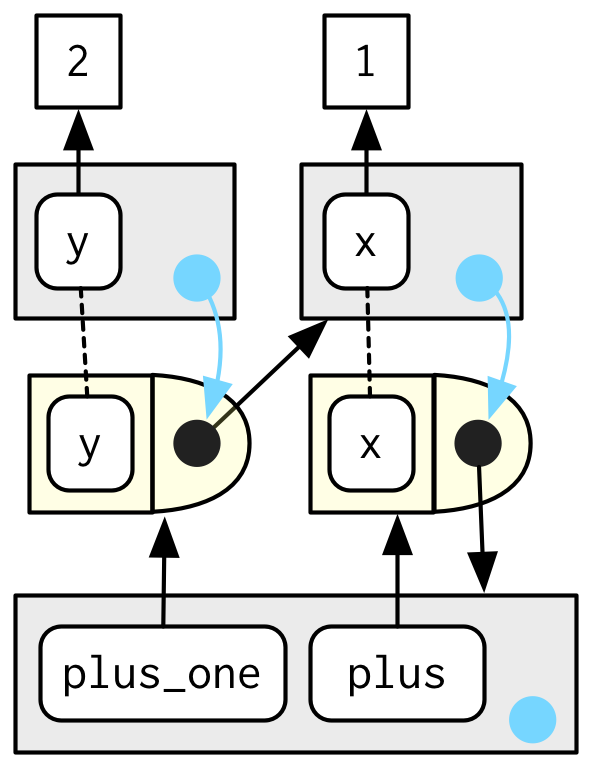
\includegraphics{diagrams/environments/closure-call} \end{center}

You'll learn more about function factories in
\protect\hyperlink{functional-programming}{functional programming}.

\subsection{Exercises}\label{exercises-8}

\begin{enumerate}
\def\labelenumi{\arabic{enumi}.}
\item
  How is \texttt{search\_envs()} different to
  \texttt{env\_parents(global\_env())}?
\item
  Draw a diagram that shows the enclosing environments of this function:

\begin{Shaded}
\begin{Highlighting}[]
\NormalTok{f1 <-}\StringTok{ }\ControlFlowTok{function}\NormalTok{(x1) \{}
\NormalTok{  f2 <-}\StringTok{ }\ControlFlowTok{function}\NormalTok{(x2) \{}
\NormalTok{    f3 <-}\StringTok{ }\ControlFlowTok{function}\NormalTok{(x3) \{}
\NormalTok{      x1 }\OperatorTok{+}\StringTok{ }\NormalTok{x2 }\OperatorTok{+}\StringTok{ }\NormalTok{x3}
\NormalTok{    \}}
    \KeywordTok{f3}\NormalTok{(}\DecValTok{3}\NormalTok{)}
\NormalTok{  \}}
  \KeywordTok{f2}\NormalTok{(}\DecValTok{2}\NormalTok{)}
\NormalTok{\}}
\KeywordTok{f1}\NormalTok{(}\DecValTok{1}\NormalTok{)}
\end{Highlighting}
\end{Shaded}
\item
  Write an enhanced version of \texttt{str()} that provides more
  information about functions. Show where the function was found and
  what environment it was defined in.
\end{enumerate}

\section{The call stack}\label{the-call-stack}

還有另一種環境稱為 \textbf{caller} environment, 可以經由
\texttt{rlang::caller\_env()}存取。. This provides the environment from
which the function was called, and hence varies based on how the
function is called, not how the function was created. As we saw above
this is a useful default whenever you write a function that takes an
environment as an argument.

::: base \texttt{parent.frame()} is equivalent to
\texttt{caller\_env()}; just note that it returns an environment, not a
frame. :::

To fully understand the caller environment we need to discuss two
related concepts: the \textbf{call stack}, which is made up of
\textbf{frames}. Executing a function creates two types of context.
You've learned about one already: the execution environment is a child
of the function environment, which is determined by where the function
was created. There's another type of context created by where the
function was called: this is called the call stack.

There are also a couple of small wrinkles when it comes to custom
evaluation. See \protect\hyperlink{eval-frame}{environments vs.~frames}
for more details.

\subsection{Simple call stacks}\label{simple-call-stacks}

Let's illustrate this with a simple sequence of calls: \texttt{f()}
calls \texttt{g()} calls \texttt{h()}.

\begin{Shaded}
\begin{Highlighting}[]
\NormalTok{f <-}\StringTok{ }\ControlFlowTok{function}\NormalTok{(x) \{}
  \KeywordTok{g}\NormalTok{(}\DataTypeTok{x =} \DecValTok{2}\NormalTok{)}
\NormalTok{\}}
\NormalTok{g <-}\StringTok{ }\ControlFlowTok{function}\NormalTok{(x) \{}
  \KeywordTok{h}\NormalTok{(}\DataTypeTok{x =} \DecValTok{3}\NormalTok{)}
\NormalTok{\}}
\NormalTok{h <-}\StringTok{ }\ControlFlowTok{function}\NormalTok{(x) \{}
  \KeywordTok{stop}\NormalTok{()}
\NormalTok{\}}
\end{Highlighting}
\end{Shaded}

The way you most commonly see a call stack in R is by looking at the
\texttt{traceback()} after an error has occured:

\begin{Shaded}
\begin{Highlighting}[]
\KeywordTok{f}\NormalTok{(}\DataTypeTok{x =} \DecValTok{1}\NormalTok{)}
\CommentTok{#> Error:}
\KeywordTok{traceback}\NormalTok{()}
\CommentTok{#> 4: stop()}
\CommentTok{#> 3: h(x = 3) }
\CommentTok{#> 2: g(x = 2)}
\CommentTok{#> 1: f(x = 1)}
\end{Highlighting}
\end{Shaded}

Instead of \texttt{stop()} + \texttt{traceback()} to understand the call
stack, we're going to use \texttt{lobstr::cst()} to print out the
\textbf{c}all \textbf{s}tack \textbf{t}ree:

\begin{Shaded}
\begin{Highlighting}[]
\NormalTok{h <-}\StringTok{ }\ControlFlowTok{function}\NormalTok{(x) \{}
\NormalTok{  lobstr}\OperatorTok{::}\KeywordTok{cst}\NormalTok{()}
\NormalTok{\}}
\KeywordTok{f}\NormalTok{(}\DataTypeTok{x =} \DecValTok{1}\NormalTok{)}
\CommentTok{#> ???}
\CommentTok{#> ???€f(x = 1)}
\CommentTok{#>   ???€g(x = 2)}
\CommentTok{#>     ???€h(x = 3)}
\CommentTok{#>       ???€lobstr::cst()}
\end{Highlighting}
\end{Shaded}

This shows us that \texttt{cst()} was called from \texttt{h()}, which
was called from \texttt{g()}, which was called from \texttt{f()}. Note
that the order is the opposite from \texttt{traceback()}. As the call
stacks get more compliated, I think it's easier to understand the
sequence of calls if you start from the beginning, rather than the end
(i.e. \texttt{f()} calls \texttt{g()}; rather than \texttt{g()} was
called by \texttt{f()}).

\subsection{Lazy evaluation}\label{lazy-evaluation}

The call stack above is simple - while you get a hint that there's some
tree-like structure involved, everything happens on a single branch.
This is typical of a call stack when all arguments are eagerly
evaluated.

Let's create a more complicated example that involves some lazy
evaluation. We'll create a sequence of functions, \texttt{a()},
\texttt{b()}, \texttt{c()}, that pass along an argument \texttt{x}.

\begin{Shaded}
\begin{Highlighting}[]
\NormalTok{a <-}\StringTok{ }\ControlFlowTok{function}\NormalTok{(x) }\KeywordTok{b}\NormalTok{(x)}
\NormalTok{b <-}\StringTok{ }\ControlFlowTok{function}\NormalTok{(x) }\KeywordTok{c}\NormalTok{(x)}
\NormalTok{c <-}\StringTok{ }\ControlFlowTok{function}\NormalTok{(x) x}

\KeywordTok{a}\NormalTok{(}\KeywordTok{f}\NormalTok{())}
\CommentTok{#> ???}
\CommentTok{#> ???€a(f())}
\CommentTok{#> ??? ???€b(x)}
\CommentTok{#> ???   ???€c(x)}
\CommentTok{#> ???€f()}
\CommentTok{#>   ???€g(x = 2)}
\CommentTok{#>     ???€h(x = 3)}
\CommentTok{#>       ???€lobstr::cst()}
\end{Highlighting}
\end{Shaded}

\texttt{x} is lazily evaluated so this tree gets two branches. In the
first branch \texttt{a()} calls \texttt{b()}, then \texttt{b()} calls
\texttt{c()}. The second branch starts when \texttt{c()} evaluates its
argument \texttt{x}. This argument is evaluated in a new branch because
the environment in which it is evaluated is the global environment, not
the environment of \texttt{c()}.

\subsection{Frames}\label{frames}

Each element of the call stack is a \textbf{frame}\footnote{NB:
  \texttt{?environment} uses frame in a different sense: ``Environments
  consist of a \emph{frame}, or collection of named objects, and a
  pointer to an enclosing environment.''. We avoid this sense of frame,
  which comes from S, because it's very specific and not widely used in
  base R. For example, the ``frame'' in \texttt{parent.frame()} is an
  execution context, not a collection of named objects.}, also known as
an evaluation context. The frame is an extremely important internal data
structure, and R code can only access a small part of the data structure
because it's so critical. A frame has three main components that are
accessible from R:

\begin{itemize}
\item
  An expression (labelled with \texttt{expr}) giving the function call.
  This is what \texttt{traceback()} prints out.
\item
  An environment (labelled with \texttt{env}), which is typically the
  execution environment of a function. There are two main exceptions:
  the environment of the global frame is the global environment, and
  calling \texttt{eval()} also generates frames, where the environment
  can be anything.
\item
  A parent, the previous call in the call stack (shown by a grey arrow).
\end{itemize}

\begin{center}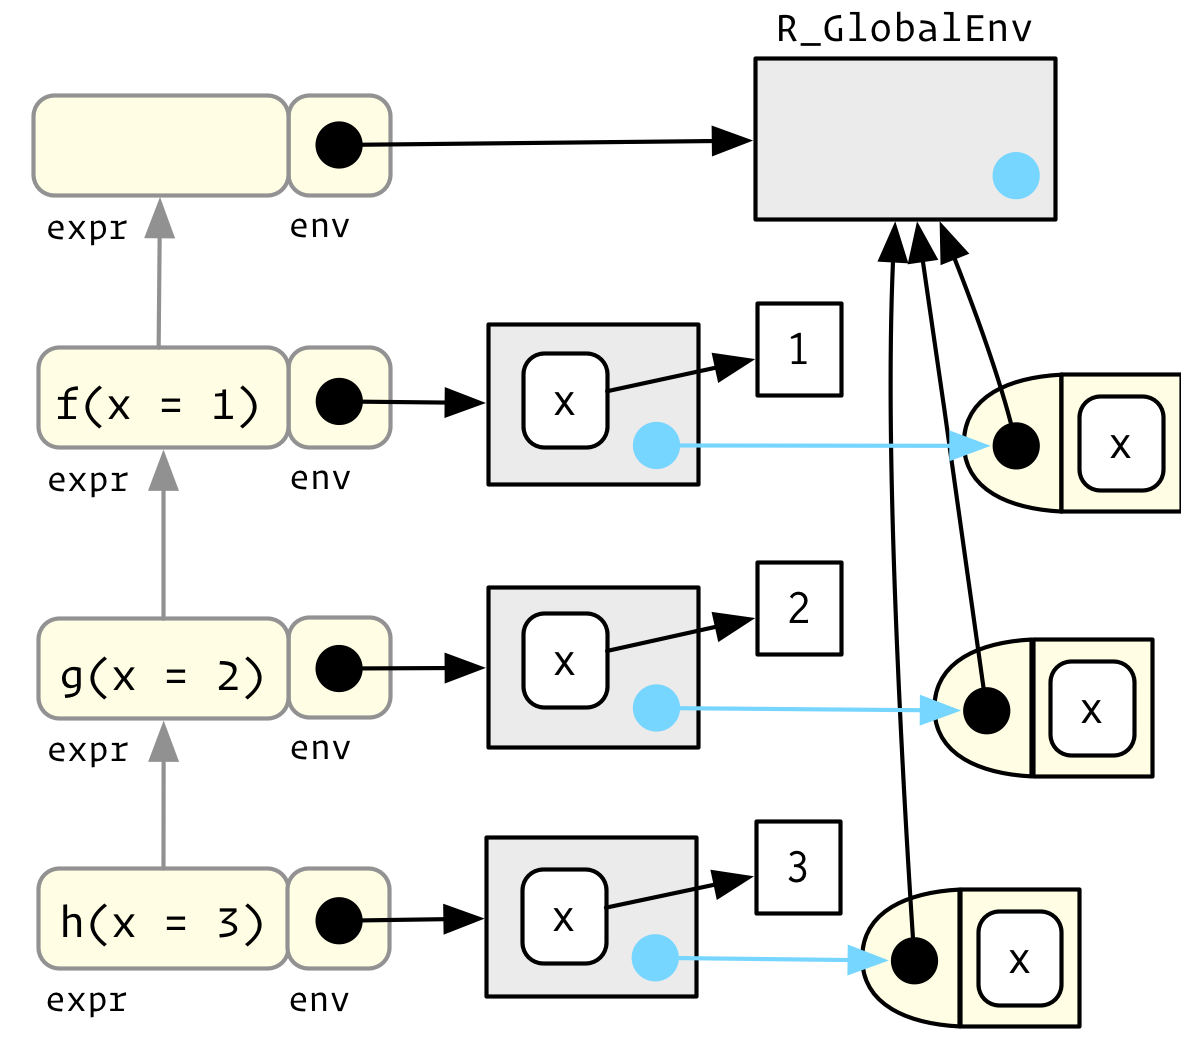
\includegraphics{diagrams/environments/calling} \end{center}

(To focus on the calling environments, I have omitted the bindings in
the global environment from \texttt{f}, \texttt{g}, and \texttt{h} to
the respective function objects.)

The frame also holds exit handlers created with \texttt{on.exit()},
restarts and handlers for the condition system, and which context to
\texttt{return()} to when a function completes. These are important for
the internal operation of R, but are not directly accessible.

\subsection{Dynamic scope}\label{dynamic-scope}

Looking up variables in the calling stack rather than in the enclosing
environment is called \textbf{dynamic scoping}. Few languages implement
dynamic scoping (Emacs Lisp is a
\href{http://www.gnu.org/software/emacs/emacs-paper.html\#SEC15}{notable
exception}.) This is because dynamic scoping makes it much harder to
reason about how a function operates: not only do you need to know how
it was defined, you also need to know the context in which it was
called. Dynamic scoping is primarily useful for developing functions
that aid interactive data analysis. It is one of the topics discussed in
\protect\hyperlink{nse}{non-standard evaluation}.

\subsection{Exercises}\label{exercises-9}

\begin{enumerate}
\def\labelenumi{\arabic{enumi}.}
\tightlist
\item
  Write a function that lists all the variables defined in the
  environment in which it was called. It should return the same results
  as \texttt{ls()}.
\end{enumerate}

\hypertarget{explicit-envs}{\section{As data
structures}\label{explicit-envs}}

As well as powering scoping, environments are also useful data
structures in their own right because they have reference semantics.
There are three common problems that they can help solve:

\begin{itemize}
\item
  \textbf{Avoiding copies of large data}. Since environments have
  reference semantics, you'll never accidentally create a copy. This
  makes it a useful vessel for large objects. Bare environments are not
  that pleasant to work with; I recommend using R6 objects instead.
  Learn more in {[}R6{]}.
\item
  \textbf{Managing state within a package}. Explicit environments are
  useful in packages because they allow you to maintain state across
  function calls. Normally, objects in a package are locked, so you
  can't modify them directly. Instead, you can do something like this:

\begin{Shaded}
\begin{Highlighting}[]
\NormalTok{my_env <-}\StringTok{ }\KeywordTok{new.env}\NormalTok{(}\DataTypeTok{parent =} \KeywordTok{emptyenv}\NormalTok{())}
\NormalTok{my_env}\OperatorTok{$}\NormalTok{a <-}\StringTok{ }\DecValTok{1}

\NormalTok{get_a <-}\StringTok{ }\ControlFlowTok{function}\NormalTok{() \{}
\NormalTok{  my_env}\OperatorTok{$}\NormalTok{a}
\NormalTok{\}}
\NormalTok{set_a <-}\StringTok{ }\ControlFlowTok{function}\NormalTok{(value) \{}
\NormalTok{  old <-}\StringTok{ }\NormalTok{my_env}\OperatorTok{$}\NormalTok{a}
\NormalTok{  my_env}\OperatorTok{$}\NormalTok{a <-}\StringTok{ }\NormalTok{value}
  \KeywordTok{invisible}\NormalTok{(old)}
\NormalTok{\}}
\end{Highlighting}
\end{Shaded}

  Returning the old value from setter functions is a good pattern
  because it makes it easier to reset the previous value in conjunction
  with \texttt{on.exit()} (see more in \protect\hyperlink{on-exit}{on
  exit}).
\item
  \textbf{As a hashmap}. A hashmap is a data structure that takes
  constant, O(1), time to find an object based on its name. Environments
  provide this behaviour by default, so can be used to simulate a
  hashmap. See the CRAN package hash for a complete development of this
  idea.
\end{itemize}

\section{\texorpdfstring{\texttt{\textless{}\textless{}-}}{\textless{}\textless{}-}}\label{section}

The ancestors of an environment have an important relationship to
\texttt{\textless{}\textless{}-}. The regular assignment arrow,
\texttt{\textless{}-}, always creates a variable in the current
environment. The deep assignment arrow,
\texttt{\textless{}\textless{}-}, never creates a variable in the
current environment, but instead modifies an existing variable found by
walking up the parent environments.

\begin{Shaded}
\begin{Highlighting}[]
\NormalTok{x <-}\StringTok{ }\DecValTok{0}
\NormalTok{f <-}\StringTok{ }\ControlFlowTok{function}\NormalTok{() \{}
\NormalTok{  x <<-}\StringTok{ }\DecValTok{1}
\NormalTok{\}}
\KeywordTok{f}\NormalTok{()}
\NormalTok{x}
\end{Highlighting}
\end{Shaded}

If \texttt{\textless{}\textless{}-} doesn't find an existing variable,
it will create one in the global environment. This is usually
undesirable, because global variables introduce non-obvious dependencies
between functions. \texttt{\textless{}\textless{}-} is most often used
in conjunction with a closure, as described in
\protect\hyperlink{closures}{Closures}.

\subsection{Exercises}\label{exercises-10}

\begin{enumerate}
\def\labelenumi{\arabic{enumi}.}
\item
  What does this function do? How does it differ from
  \texttt{\textless{}\textless{}-} and why might you prefer it?

\begin{Shaded}
\begin{Highlighting}[]
\NormalTok{rebind <-}\StringTok{ }\ControlFlowTok{function}\NormalTok{(name, value, }\DataTypeTok{env =} \KeywordTok{caller_env}\NormalTok{()) \{}
  \ControlFlowTok{if}\NormalTok{ (}\KeywordTok{identical}\NormalTok{(env, }\KeywordTok{empty_env}\NormalTok{())) \{}
    \KeywordTok{stop}\NormalTok{(}\StringTok{"Can't find `"}\NormalTok{, name, }\StringTok{"`"}\NormalTok{, }\DataTypeTok{call. =} \OtherTok{FALSE}\NormalTok{)}
\NormalTok{  \} }\ControlFlowTok{else} \ControlFlowTok{if}\NormalTok{ (}\KeywordTok{env_has}\NormalTok{(env, name)) \{}
    \KeywordTok{env_poke}\NormalTok{(env, name, value)}
\NormalTok{  \} }\ControlFlowTok{else}\NormalTok{ \{}
    \KeywordTok{rebind}\NormalTok{(name, value, }\KeywordTok{env_parent}\NormalTok{(env))}
\NormalTok{  \}}
\NormalTok{\}}
\KeywordTok{rebind}\NormalTok{(}\StringTok{"a"}\NormalTok{, }\DecValTok{10}\NormalTok{)}
\end{Highlighting}
\end{Shaded}

\begin{Shaded}
\begin{Highlighting}[]
\NormalTok{a <-}\StringTok{ }\DecValTok{5}
\KeywordTok{rebind}\NormalTok{(}\StringTok{"a"}\NormalTok{, }\DecValTok{10}\NormalTok{)}
\NormalTok{a}
\end{Highlighting}
\end{Shaded}
\end{enumerate}

\hypertarget{env-answers}{\section{Quiz answers}\label{env-answers}}

\begin{enumerate}
\def\labelenumi{\arabic{enumi}.}
\item
  There are four ways: every object in an environment must have a name;
  order doesn't matter; environments have parents; environments have
  reference semantics.
\item
  The parent of the global environment is the last package that you
  loaded. The only environment that doesn't have a parent is the empty
  environment.
\item
  The enclosing environment of a function is the environment where it
  was created. It determines where a function looks for variables.
\item
  Use \texttt{caller\_env()} or \texttt{parent.frame()}.
\item
  \texttt{\textless{}-} always creates a binding in the current
  environment; \texttt{\textless{}\textless{}-} rebinds an existing name
  in a parent of the current environment.
\end{enumerate}

\subsection{term}\label{term}

\hypertarget{global-environment}{\paragraph{global environment
:總體環境}\label{global-environment}}

\paragraph{package environments}\label{package-environments}

\hypertarget{imports-environment}{\paragraph{imports
environment}\label{imports-environment}}

\chapter{Basic Plot}\label{basic-plot}

\section{reference}\label{reference-1}

\href{https://www.statmethods.net/graphs/creating.html}{Quric R}

windows() \#\# create window to plot your file \#\# \ldots{} your
plotting code here \ldots{}

\begin{quote}
dev.off()
\end{quote}

Note:

This will delete your current plots in the RStudio Plots Pane. If you
have multiple graphics devices open, repeat this command until the
output displays null device.

\section{basic}\label{basic}

Creating a Graph In R, graphs are typically created interactively.

\subsection{Creating a Graph}\label{creating-a-graph}

\begin{Shaded}
\begin{Highlighting}[]
\KeywordTok{attach}\NormalTok{(mtcars)}
\end{Highlighting}
\end{Shaded}

\begin{verbatim}
The following object is masked from package:ggplot2:

    mpg
\end{verbatim}

\begin{Shaded}
\begin{Highlighting}[]
\KeywordTok{plot}\NormalTok{(wt, mpg) }
\KeywordTok{abline}\NormalTok{(}\KeywordTok{lm}\NormalTok{(mpg}\OperatorTok{~}\NormalTok{wt))}
\KeywordTok{title}\NormalTok{(}\StringTok{"Regression of MPG on Weight"}\NormalTok{)}
\end{Highlighting}
\end{Shaded}

\begin{center}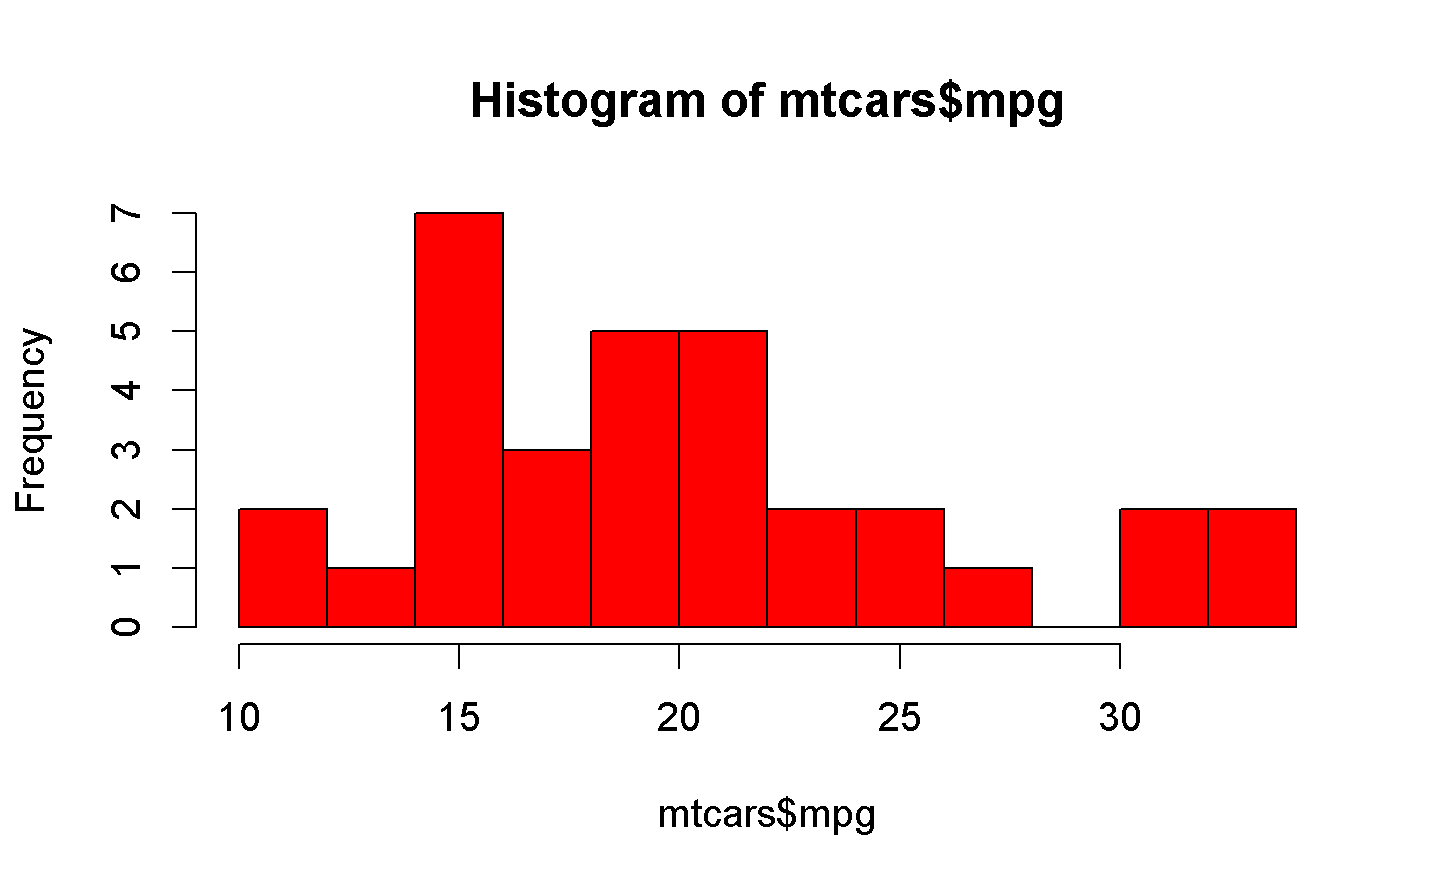
\includegraphics[width=0.7\linewidth]{rmi_copy_test_files/figure-latex/unnamed-chunk-360-1} \end{center}

The plot( ) function opens a graph window and plots weight vs.~miles per
gallon. The next line of code adds a regression line to this graph. The
final line adds a title.

plot example click to view

Saving Graphs\\
You can save the graph in a variety of formats from the menu File
-\textgreater{} Save As.

You can also save the graph via code using one of the following
functions.

\begin{longtable}[]{@{}ll@{}}
\toprule
Function & Output to\tabularnewline
\midrule
\endhead
pdf(``mygraph.pdf'') & pdf file\tabularnewline
win.metafile(``mygraph.wmf'') & windows metafile\tabularnewline
png(``mygraph.png'') & png file\tabularnewline
jpeg(``mygraph.jpg'') & jpeg file\tabularnewline
bmp(``mygraph.bmp'') & bmp file\tabularnewline
postscript(``mygraph.ps'') & postscript file\tabularnewline
\bottomrule
\end{longtable}

See input/output for details.

Viewing Several Graphs Creating a new graph by issuing a high level
plotting command (plot, hist, boxplot, etc.) will typically overwrite a
previous graph. To avoid this, open a new graph window before creating a
new graph. To open a new graph window use one of the functions below.

\begin{longtable}[]{@{}ll@{}}
\toprule
Function & Platform\tabularnewline
\midrule
\endhead
windows() & Windows\tabularnewline
X11() & Unix\tabularnewline
quartz() & Mac\tabularnewline
\bottomrule
\end{longtable}

You can have multiple graph windows open at one time. See help(dev.cur)
for more details.

\section{Histograms and Density
Plots}\label{histograms-and-density-plots}

\subsection{Histograms}\label{histograms}

You can create histograms with the function hist(x) where x is a numeric
vector of values to be plotted. The option freq=FALSE plots probability
densities instead of frequencies. The option breaks= controls the number
of bins.

\subsubsection{Simple Histogram}\label{simple-histogram}

\begin{Shaded}
\begin{Highlighting}[]
\KeywordTok{hist}\NormalTok{(mtcars}\OperatorTok{$}\NormalTok{mpg)}
\end{Highlighting}
\end{Shaded}

\begin{center}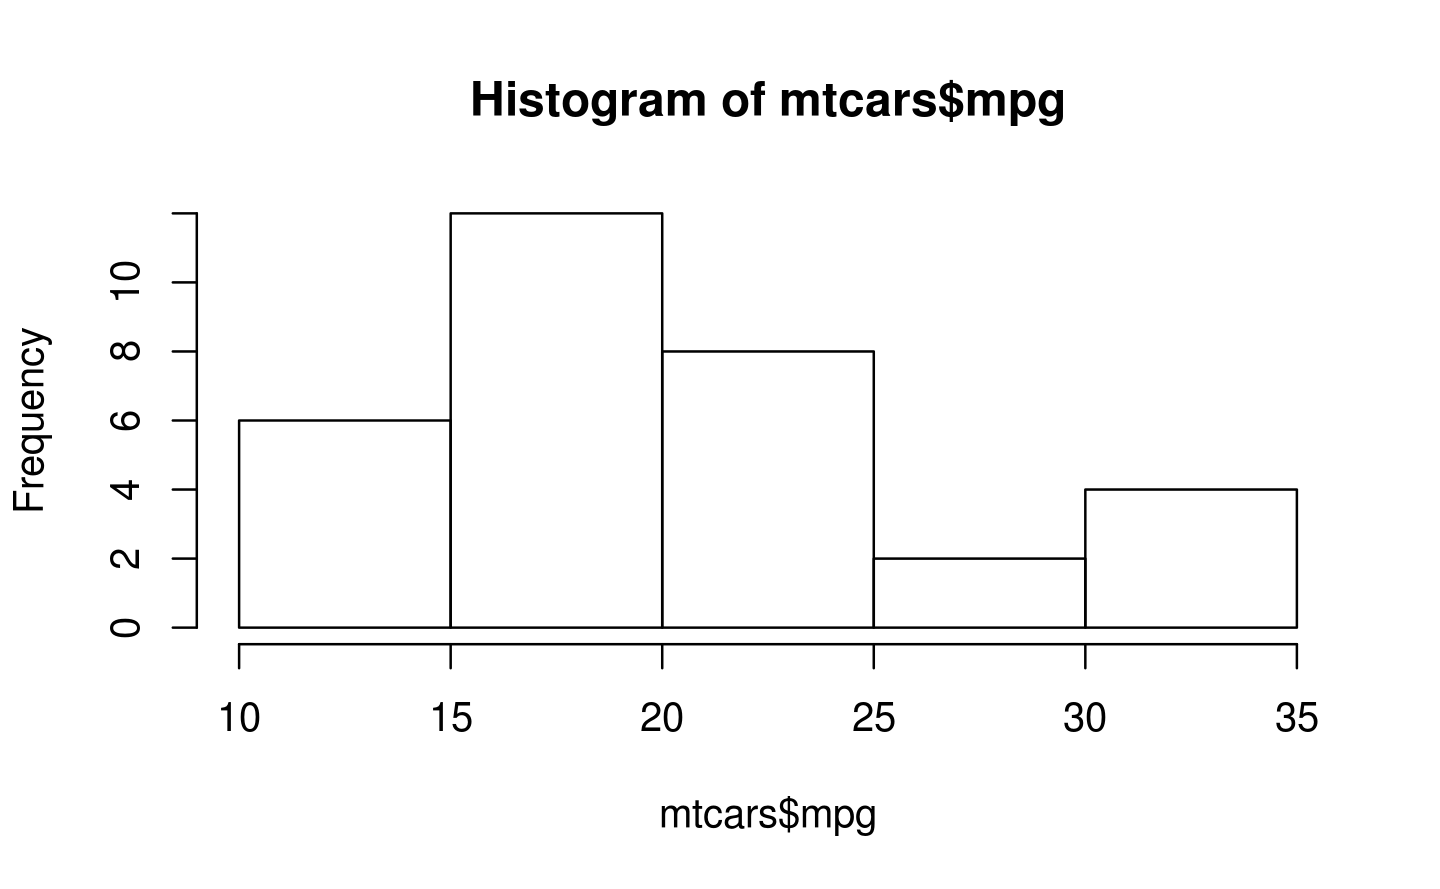
\includegraphics[width=0.7\linewidth]{rmi_copy_test_files/figure-latex/unnamed-chunk-361-1} \end{center}

simple histogram click to view

\subsubsection{Colored Histogram with Different Number of
Bins}\label{colored-histogram-with-different-number-of-bins}

\begin{Shaded}
\begin{Highlighting}[]
\KeywordTok{hist}\NormalTok{(mtcars}\OperatorTok{$}\NormalTok{mpg, }\DataTypeTok{breaks=}\DecValTok{12}\NormalTok{, }\DataTypeTok{col=}\StringTok{"red"}\NormalTok{)}
\end{Highlighting}
\end{Shaded}

\begin{center}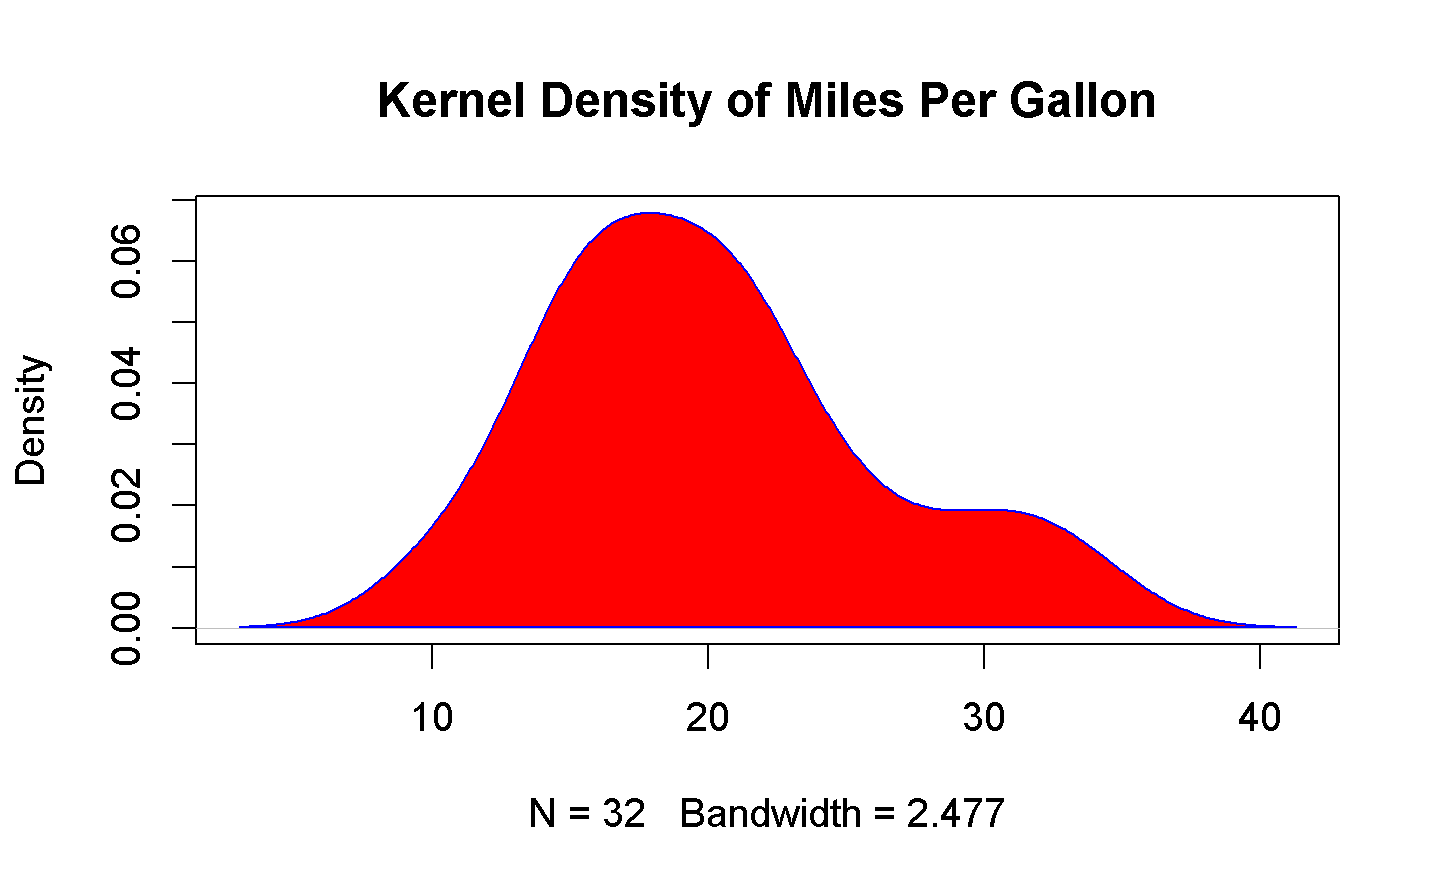
\includegraphics[width=0.7\linewidth]{rmi_copy_test_files/figure-latex/unnamed-chunk-362-1} \end{center}

colored histogram click to view

\subsubsection{Add a Normal Curve (Thanks to Peter
Dalgaard)}\label{add-a-normal-curve-thanks-to-peter-dalgaard}

\begin{Shaded}
\begin{Highlighting}[]
\NormalTok{x <-}\StringTok{ }\NormalTok{mtcars}\OperatorTok{$}\NormalTok{mpg }
\NormalTok{h<-}\KeywordTok{hist}\NormalTok{(x, }\DataTypeTok{breaks=}\DecValTok{10}\NormalTok{, }\DataTypeTok{col=}\StringTok{"red"}\NormalTok{, }\DataTypeTok{xlab=}\StringTok{"Miles Per Gallon"}\NormalTok{, }
    \DataTypeTok{main=}\StringTok{"Histogram with Normal Curve"}\NormalTok{) }
\NormalTok{xfit<-}\KeywordTok{seq}\NormalTok{(}\KeywordTok{min}\NormalTok{(x),}\KeywordTok{max}\NormalTok{(x),}\DataTypeTok{length=}\DecValTok{40}\NormalTok{) }
\NormalTok{yfit<-}\KeywordTok{dnorm}\NormalTok{(xfit,}\DataTypeTok{mean=}\KeywordTok{mean}\NormalTok{(x),}\DataTypeTok{sd=}\KeywordTok{sd}\NormalTok{(x)) }
\NormalTok{yfit <-}\StringTok{ }\NormalTok{yfit}\OperatorTok{*}\KeywordTok{diff}\NormalTok{(h}\OperatorTok{$}\NormalTok{mids[}\DecValTok{1}\OperatorTok{:}\DecValTok{2}\NormalTok{])}\OperatorTok{*}\KeywordTok{length}\NormalTok{(x) }
\KeywordTok{lines}\NormalTok{(xfit, yfit, }\DataTypeTok{col=}\StringTok{"blue"}\NormalTok{, }\DataTypeTok{lwd=}\DecValTok{2}\NormalTok{)}
\end{Highlighting}
\end{Shaded}

\begin{center}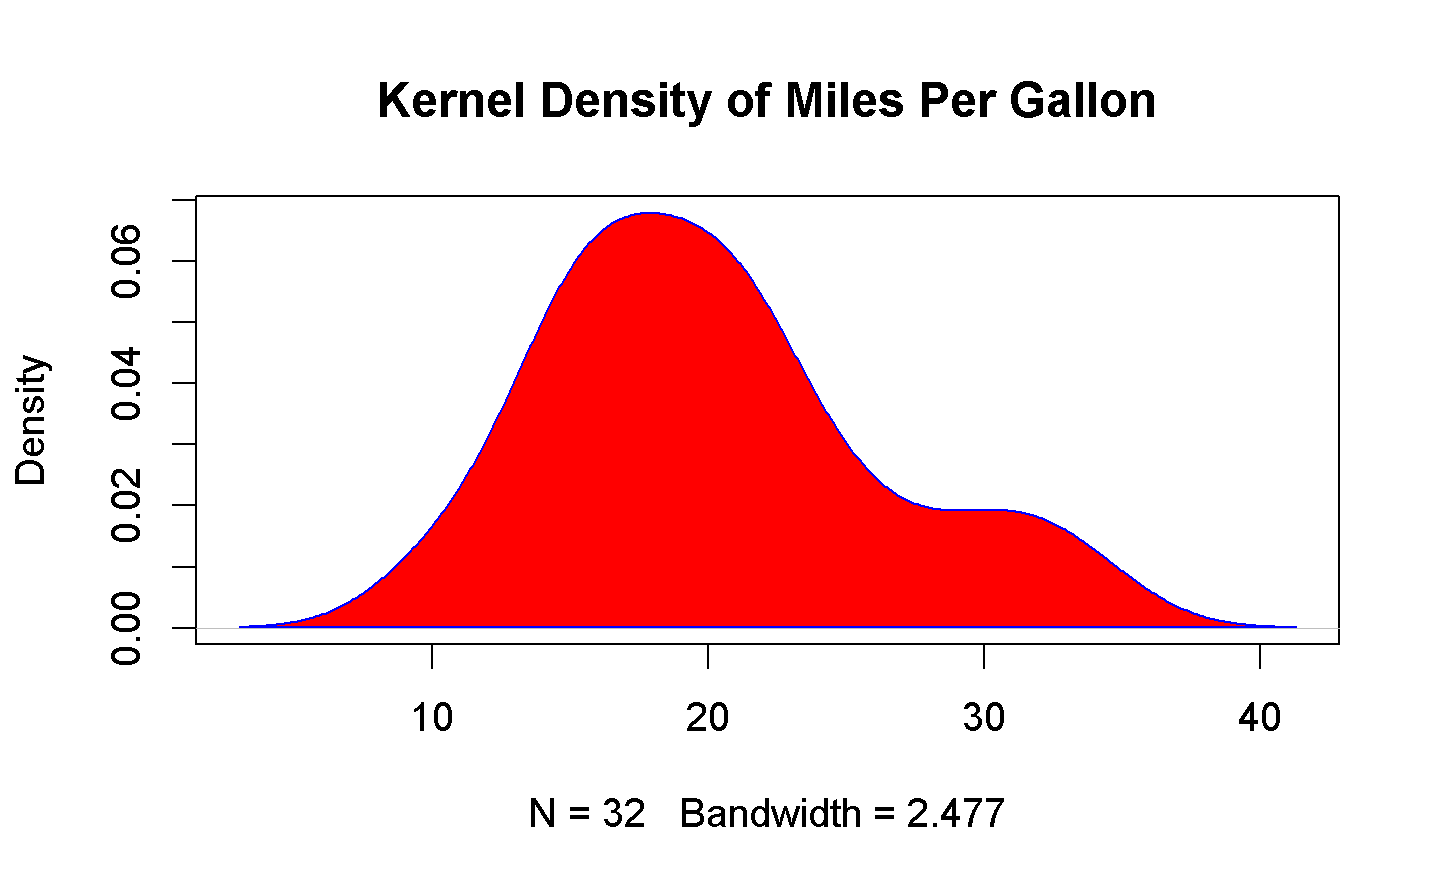
\includegraphics[width=0.7\linewidth]{rmi_copy_test_files/figure-latex/unnamed-chunk-363-1} \end{center}

histogram with normal curve click to view

Histograms can be a poor method for determining the shape of a
distribution because it is so strongly affected by the number of bins
used.

To practice making a density plot with the hist() function, try this
exercise.

\subsection{Kernel Density Plot}\label{kernel-density-plot}

Kernal density plots are usually a much more effective way to view the
distribution of a variable. Create the plot using plot(density(x)) where
x is a numeric vector.

\begin{Shaded}
\begin{Highlighting}[]
\NormalTok{d <-}\StringTok{ }\KeywordTok{density}\NormalTok{(mtcars}\OperatorTok{$}\NormalTok{mpg) }\CommentTok{# returns the density data }
\KeywordTok{plot}\NormalTok{(d) }\CommentTok{# plots the results}
\end{Highlighting}
\end{Shaded}

\begin{center}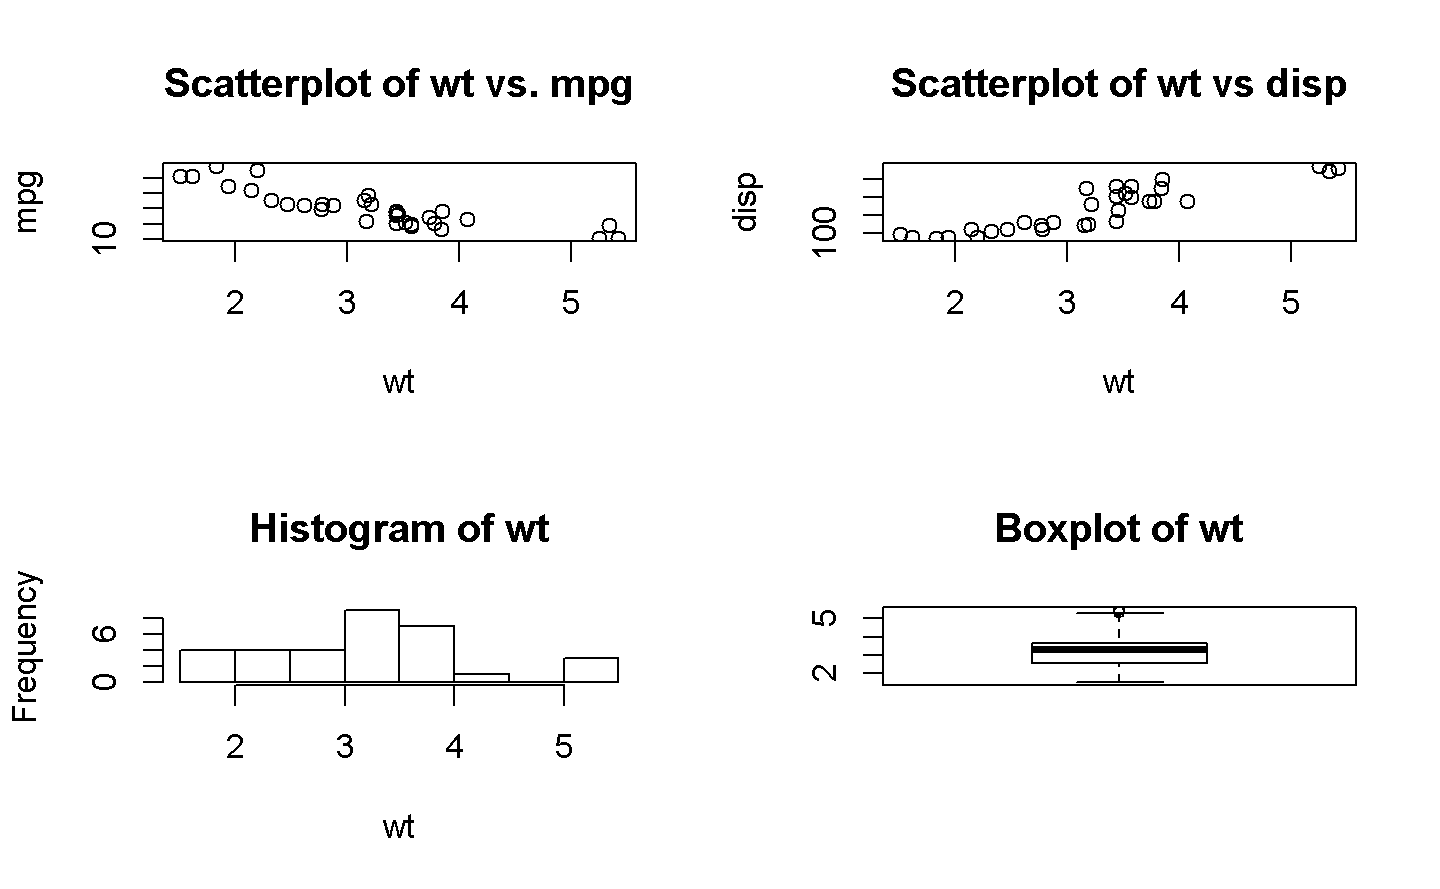
\includegraphics[width=0.7\linewidth]{rmi_copy_test_files/figure-latex/unnamed-chunk-364-1} \end{center}

simple density plot click to view

\subsubsection{Filled Density Plot}\label{filled-density-plot}

\begin{Shaded}
\begin{Highlighting}[]
\NormalTok{d <-}\StringTok{ }\KeywordTok{density}\NormalTok{(mtcars}\OperatorTok{$}\NormalTok{mpg)}
\KeywordTok{plot}\NormalTok{(d, }\DataTypeTok{main=}\StringTok{"Kernel Density of Miles Per Gallon"}\NormalTok{)}
\KeywordTok{polygon}\NormalTok{(d, }\DataTypeTok{col=}\StringTok{"red"}\NormalTok{, }\DataTypeTok{border=}\StringTok{"blue"}\NormalTok{)}
\end{Highlighting}
\end{Shaded}

\begin{center}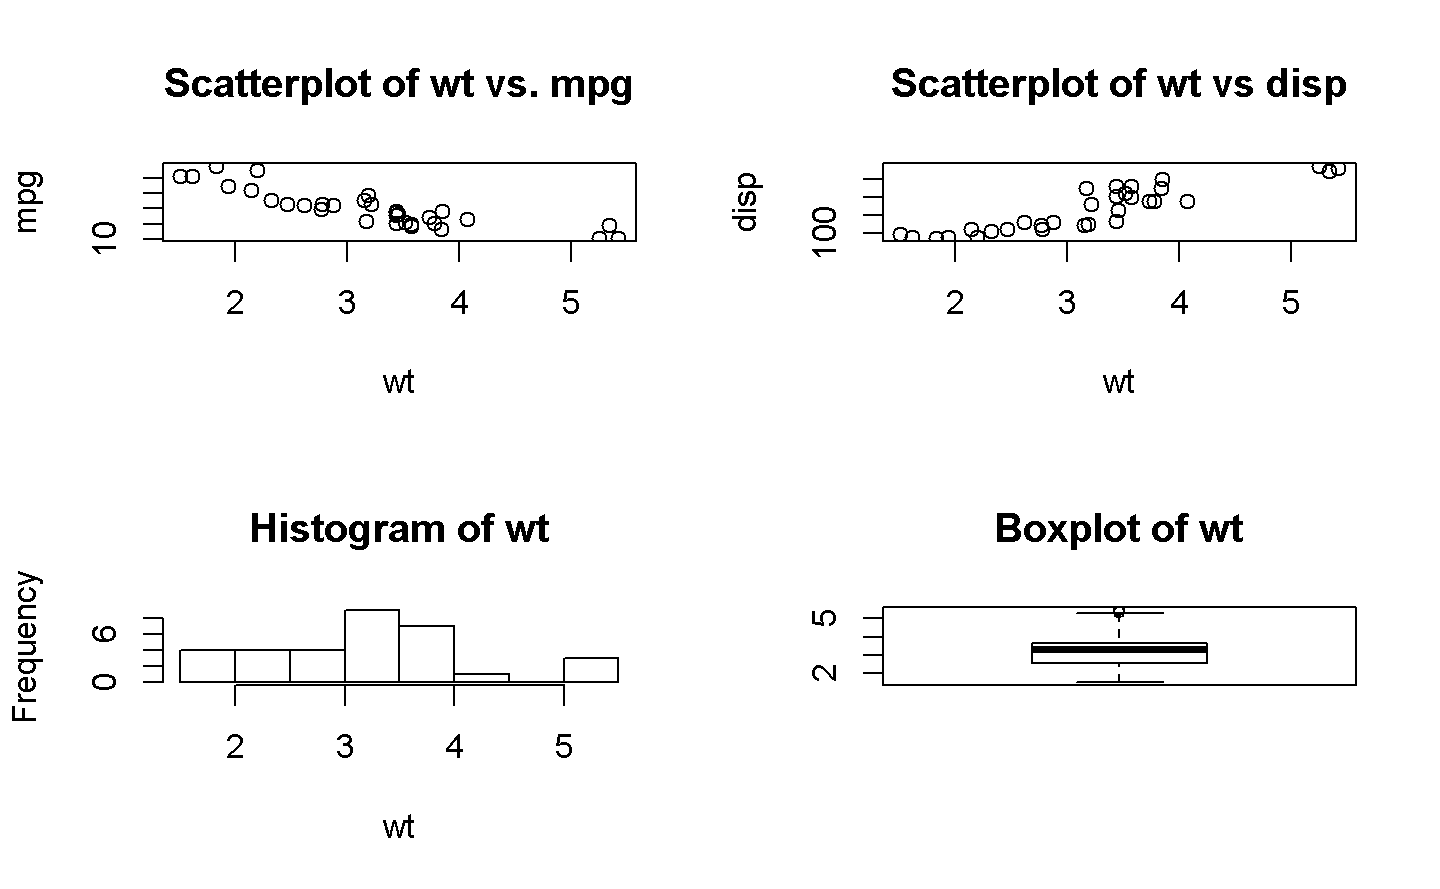
\includegraphics[width=0.7\linewidth]{rmi_copy_test_files/figure-latex/unnamed-chunk-365-1} \end{center}

colored density plot click to view

\subsection{Comparing Groups VIA Kernal
Density}\label{comparing-groups-via-kernal-density}

The sm.density.compare( ) function in the sm package allows you to
superimpose the kernal density plots of two or more groups. The format
is sm.density.compare(x, factor) where x is a numeric vector and factor
is the grouping variable.

\subsubsection{Compare MPG distributions for cars with 4,6, or 8
cylinders}\label{compare-mpg-distributions-for-cars-with-46-or-8-cylinders}

\begin{Shaded}
\begin{Highlighting}[]
\KeywordTok{library}\NormalTok{(sm)}
\KeywordTok{attach}\NormalTok{(mtcars)}

\CommentTok{#create value labels }
\NormalTok{cyl.f <-}\StringTok{ }\KeywordTok{factor}\NormalTok{(cyl, }\DataTypeTok{levels=} \KeywordTok{c}\NormalTok{(}\DecValTok{4}\NormalTok{,}\DecValTok{6}\NormalTok{,}\DecValTok{8}\NormalTok{),}
  \DataTypeTok{labels =} \KeywordTok{c}\NormalTok{(}\StringTok{"4 cylinder"}\NormalTok{, }\StringTok{"6 cylinder"}\NormalTok{, }\StringTok{"8 cylinder"}\NormalTok{)) }

\CommentTok{#plot densities }
\KeywordTok{sm.density.compare}\NormalTok{(mpg, cyl, }\DataTypeTok{xlab=}\StringTok{"Miles Per Gallon"}\NormalTok{)}
\KeywordTok{title}\NormalTok{(}\DataTypeTok{main=}\StringTok{"MPG Distribution by Car Cylinders"}\NormalTok{)}

\CommentTok{#add legend via mouse click}
\NormalTok{colfill<-}\KeywordTok{c}\NormalTok{(}\DecValTok{2}\OperatorTok{:}\NormalTok{(}\DecValTok{2}\OperatorTok{+}\KeywordTok{length}\NormalTok{(}\KeywordTok{levels}\NormalTok{(cyl.f)))) }
\KeywordTok{legend}\NormalTok{(}\KeywordTok{locator}\NormalTok{(}\DecValTok{1}\NormalTok{), }\KeywordTok{levels}\NormalTok{(cyl.f), }\DataTypeTok{fill=}\NormalTok{colfill)}
\end{Highlighting}
\end{Shaded}

\section{Combining Plots}\label{combining-plots}

R makes it easy to combine multiple plots into one overall graph, using
either the par( ) or layout( ) function.

With the par( ) function, you can include the option mfrow=c(nrows,
ncols) to create a matrix of nrows x ncols plots that are filled in by
row. mfcol=c(nrows, ncols) fills in the matrix by columns.

\begin{Shaded}
\begin{Highlighting}[]
\CommentTok{#4 figures arranged in 2 rows and 2 columns}

\KeywordTok{attach}\NormalTok{(mtcars)}
\end{Highlighting}
\end{Shaded}

\begin{verbatim}
The following objects are masked from mtcars (pos = 3):

    am, carb, cyl, disp, drat, gear, hp, mpg, qsec, vs, wt
\end{verbatim}

\begin{verbatim}
The following object is masked from package:ggplot2:

    mpg
\end{verbatim}

\begin{Shaded}
\begin{Highlighting}[]
\KeywordTok{par}\NormalTok{(}\DataTypeTok{mfrow=}\KeywordTok{c}\NormalTok{(}\DecValTok{2}\NormalTok{,}\DecValTok{2}\NormalTok{))}
\KeywordTok{plot}\NormalTok{(wt,mpg, }\DataTypeTok{main=}\StringTok{"Scatterplot of wt vs. mpg"}\NormalTok{)}
\KeywordTok{plot}\NormalTok{(wt,disp, }\DataTypeTok{main=}\StringTok{"Scatterplot of wt vs disp"}\NormalTok{)}
\KeywordTok{hist}\NormalTok{(wt, }\DataTypeTok{main=}\StringTok{"Histogram of wt"}\NormalTok{)}
\KeywordTok{boxplot}\NormalTok{(wt, }\DataTypeTok{main=}\StringTok{"Boxplot of wt"}\NormalTok{)}
\KeywordTok{dev.off}\NormalTok{()}
\end{Highlighting}
\end{Shaded}

\begin{center}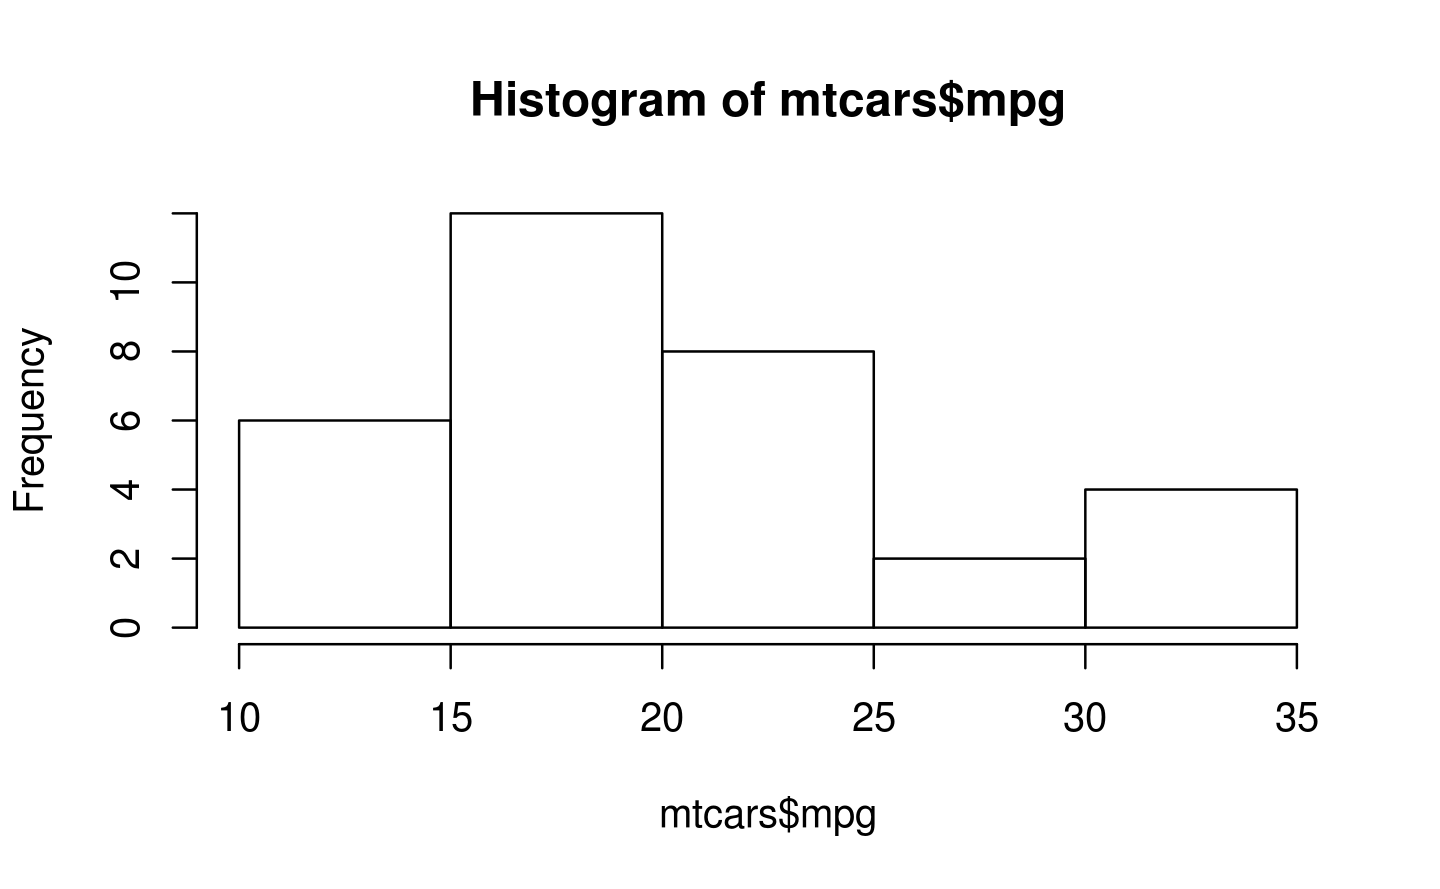
\includegraphics[width=0.7\linewidth]{rmi_copy_test_files/figure-latex/unnamed-chunk-367-1} \end{center}

2 x2 layout click to view

\begin{Shaded}
\begin{Highlighting}[]
\CommentTok{# 3 figures arranged in 3 rows and 1 column}

\KeywordTok{attach}\NormalTok{(mtcars)}
\end{Highlighting}
\end{Shaded}

\begin{verbatim}
The following objects are masked from mtcars (pos = 3):

    am, carb, cyl, disp, drat, gear, hp, mpg, qsec, vs, wt
\end{verbatim}

\begin{verbatim}
The following objects are masked from mtcars (pos = 4):

    am, carb, cyl, disp, drat, gear, hp, mpg, qsec, vs, wt
\end{verbatim}

\begin{verbatim}
The following object is masked from package:ggplot2:

    mpg
\end{verbatim}

\begin{Shaded}
\begin{Highlighting}[]
\KeywordTok{par}\NormalTok{(}\DataTypeTok{mfrow=}\KeywordTok{c}\NormalTok{(}\DecValTok{3}\NormalTok{,}\DecValTok{1}\NormalTok{)) }
\KeywordTok{hist}\NormalTok{(wt)}
\KeywordTok{hist}\NormalTok{(mpg)}
\KeywordTok{hist}\NormalTok{(disp)}
\KeywordTok{dev.off}\NormalTok{()}
\end{Highlighting}
\end{Shaded}

\begin{center}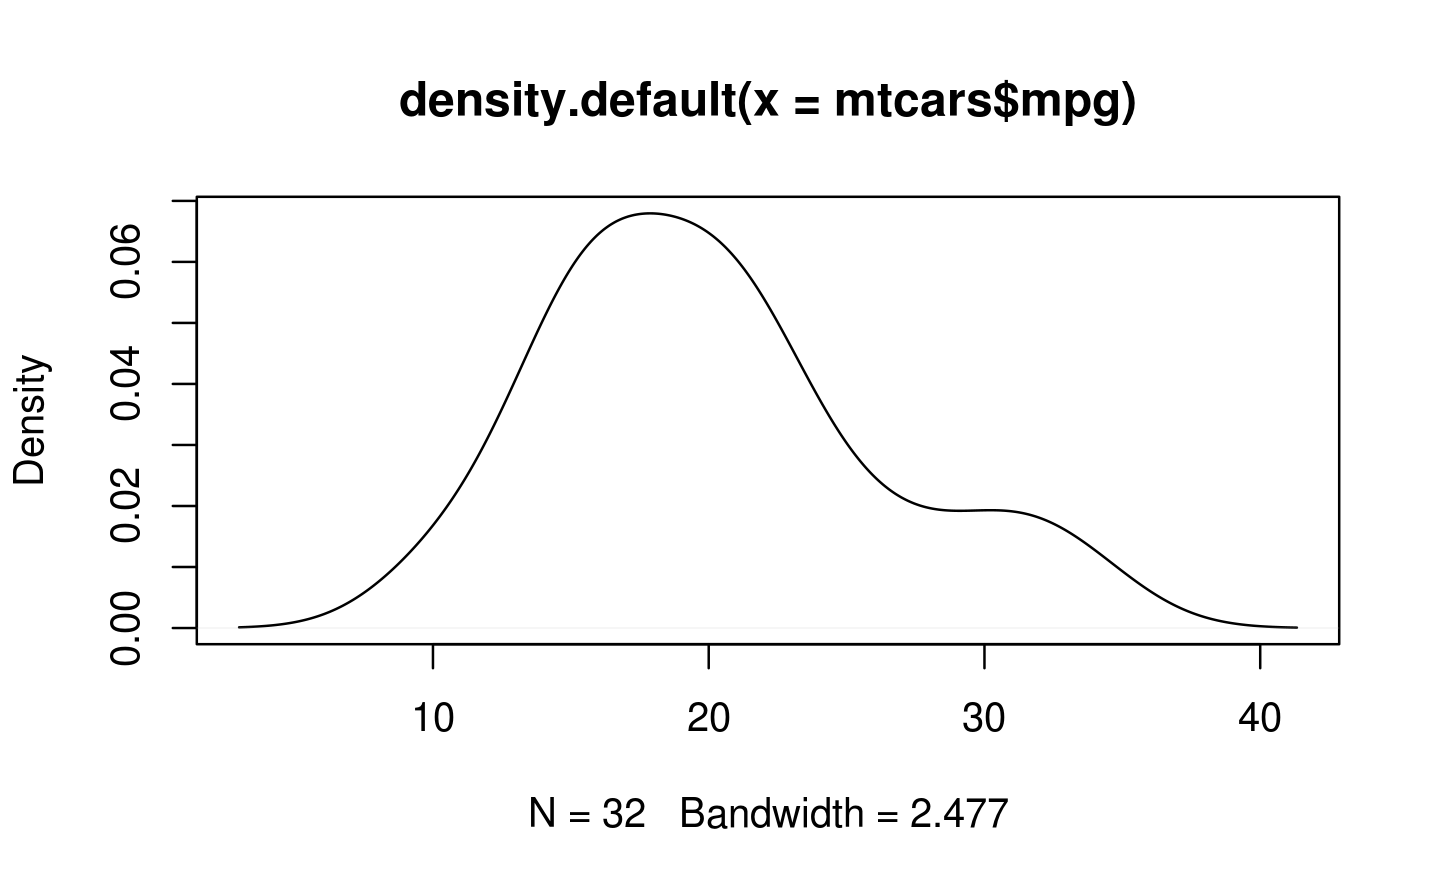
\includegraphics[width=0.7\linewidth]{rmi_copy_test_files/figure-latex/unnamed-chunk-368-1} \end{center}

3 x 1 layout

函數 layout( ) 的使用方法為 layout(mat) 其中 mat
的元素用來指定圖形號碼。例如分成4個格子,順序為左右上下(byrow=TRUE)
1在第一ROW,占用{[}1,1{]}-{[}1,2{]},2,3,分別占用{[}2,1{]}和{[}2,2{]}

\begin{Shaded}
\begin{Highlighting}[]
\CommentTok{# One figure in row 1 and two figures in row 2}
 
\KeywordTok{attach}\NormalTok{(mtcars)}
\end{Highlighting}
\end{Shaded}

\begin{verbatim}
The following objects are masked from mtcars (pos = 3):

    am, carb, cyl, disp, drat, gear, hp, mpg, qsec, vs, wt
\end{verbatim}

\begin{verbatim}
The following objects are masked from mtcars (pos = 4):

    am, carb, cyl, disp, drat, gear, hp, mpg, qsec, vs, wt
\end{verbatim}

\begin{verbatim}
The following objects are masked from mtcars (pos = 5):

    am, carb, cyl, disp, drat, gear, hp, mpg, qsec, vs, wt
\end{verbatim}

\begin{verbatim}
The following object is masked from package:ggplot2:

    mpg
\end{verbatim}

\begin{Shaded}
\begin{Highlighting}[]
\KeywordTok{layout}\NormalTok{(}\KeywordTok{matrix}\NormalTok{(}\KeywordTok{c}\NormalTok{(}\DecValTok{1}\NormalTok{,}\DecValTok{1}\NormalTok{,}\DecValTok{2}\NormalTok{,}\DecValTok{3}\NormalTok{), }\DecValTok{2}\NormalTok{, }\DecValTok{2}\NormalTok{, }\DataTypeTok{byrow =} \OtherTok{TRUE}\NormalTok{))}
\KeywordTok{hist}\NormalTok{(wt)}
\KeywordTok{hist}\NormalTok{(mpg)}
\KeywordTok{hist}\NormalTok{(disp)}
\KeywordTok{dev.off}\NormalTok{()}
\end{Highlighting}
\end{Shaded}

\begin{center}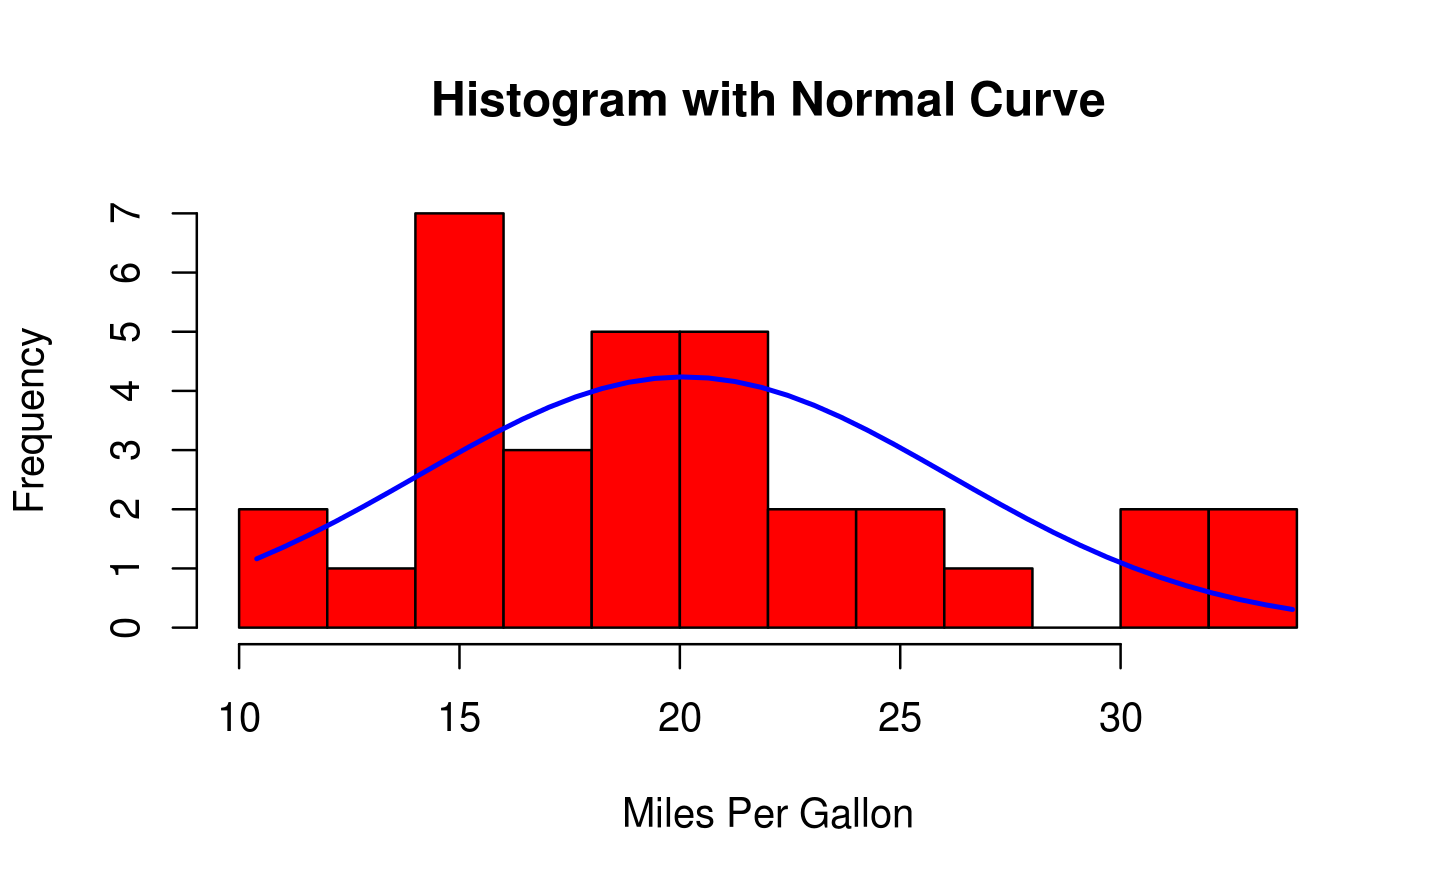
\includegraphics[width=0.7\linewidth]{rmi_copy_test_files/figure-latex/unnamed-chunk-369-1} \end{center}

Optionally, you can include widths= and heights= options in the layout(
) function to control the size of each figure more precisely. These
options have the form widths= a vector of values for the widths of
columns heights= a vector of values for the heights of rows.

Relative widths are specified with numeric values. Absolute widths (in
centimetres) are specified with the lcm() function.

::: sidebar note: par(mar) 列出margin\\
par(mar=c(1,1,1,1)) 更動margin

錯誤於plot.new() : figure margins too large

有兩個原因:1 是畫布過小 2,當前畫布的上下左右距離過大 解決第二個原因

默認的畫布上邊款的距離為: 預設為 c(5, 4, 4, 2) + 0.1. 對應 c(bottom,
left, top, right) 我們可以講其設置為0.

op \textless{}- par(mar = rep(0, 4)) \# op 之前的margin = 5.1 4.1 4.1
2.1\\
plot.new() \# 畫圖\\
par(op) \# 改回原先的margin

:::

\begin{Shaded}
\begin{Highlighting}[]
\KeywordTok{par}\NormalTok{(}\DataTypeTok{mar =} \KeywordTok{rep}\NormalTok{(}\DecValTok{2}\NormalTok{, }\DecValTok{4}\NormalTok{)) }
\CommentTok{# One figure in row 1 and two figures in row 2}
\CommentTok{# row 1 is 1/3 the height of row 2}
\CommentTok{# column 2 is 1/4 the width of the column 1 }
\KeywordTok{attach}\NormalTok{(mtcars)}
\end{Highlighting}
\end{Shaded}

\begin{verbatim}
The following objects are masked from mtcars (pos = 3):

    am, carb, cyl, disp, drat, gear, hp, mpg, qsec, vs, wt
\end{verbatim}

\begin{verbatim}
The following objects are masked from mtcars (pos = 4):

    am, carb, cyl, disp, drat, gear, hp, mpg, qsec, vs, wt
\end{verbatim}

\begin{verbatim}
The following objects are masked from mtcars (pos = 5):

    am, carb, cyl, disp, drat, gear, hp, mpg, qsec, vs, wt
\end{verbatim}

\begin{verbatim}
The following objects are masked from mtcars (pos = 6):

    am, carb, cyl, disp, drat, gear, hp, mpg, qsec, vs, wt
\end{verbatim}

\begin{verbatim}
The following object is masked from package:ggplot2:

    mpg
\end{verbatim}

\begin{Shaded}
\begin{Highlighting}[]
\KeywordTok{layout}\NormalTok{(}\KeywordTok{matrix}\NormalTok{(}\KeywordTok{c}\NormalTok{(}\DecValTok{1}\NormalTok{,}\DecValTok{1}\NormalTok{,}\DecValTok{2}\NormalTok{,}\DecValTok{3}\NormalTok{), }\DecValTok{2}\NormalTok{, }\DecValTok{2}\NormalTok{, }\DataTypeTok{byrow =} \OtherTok{TRUE}\NormalTok{), }
    \DataTypeTok{widths=}\KeywordTok{c}\NormalTok{(}\DecValTok{3}\NormalTok{,}\DecValTok{1}\NormalTok{), }\DataTypeTok{heights=}\KeywordTok{c}\NormalTok{(}\DecValTok{1}\NormalTok{,}\DecValTok{2}\NormalTok{))}
\KeywordTok{hist}\NormalTok{(wt)}
\KeywordTok{hist}\NormalTok{(mpg)}
\KeywordTok{hist}\NormalTok{(disp)}
\end{Highlighting}
\end{Shaded}

\begin{center}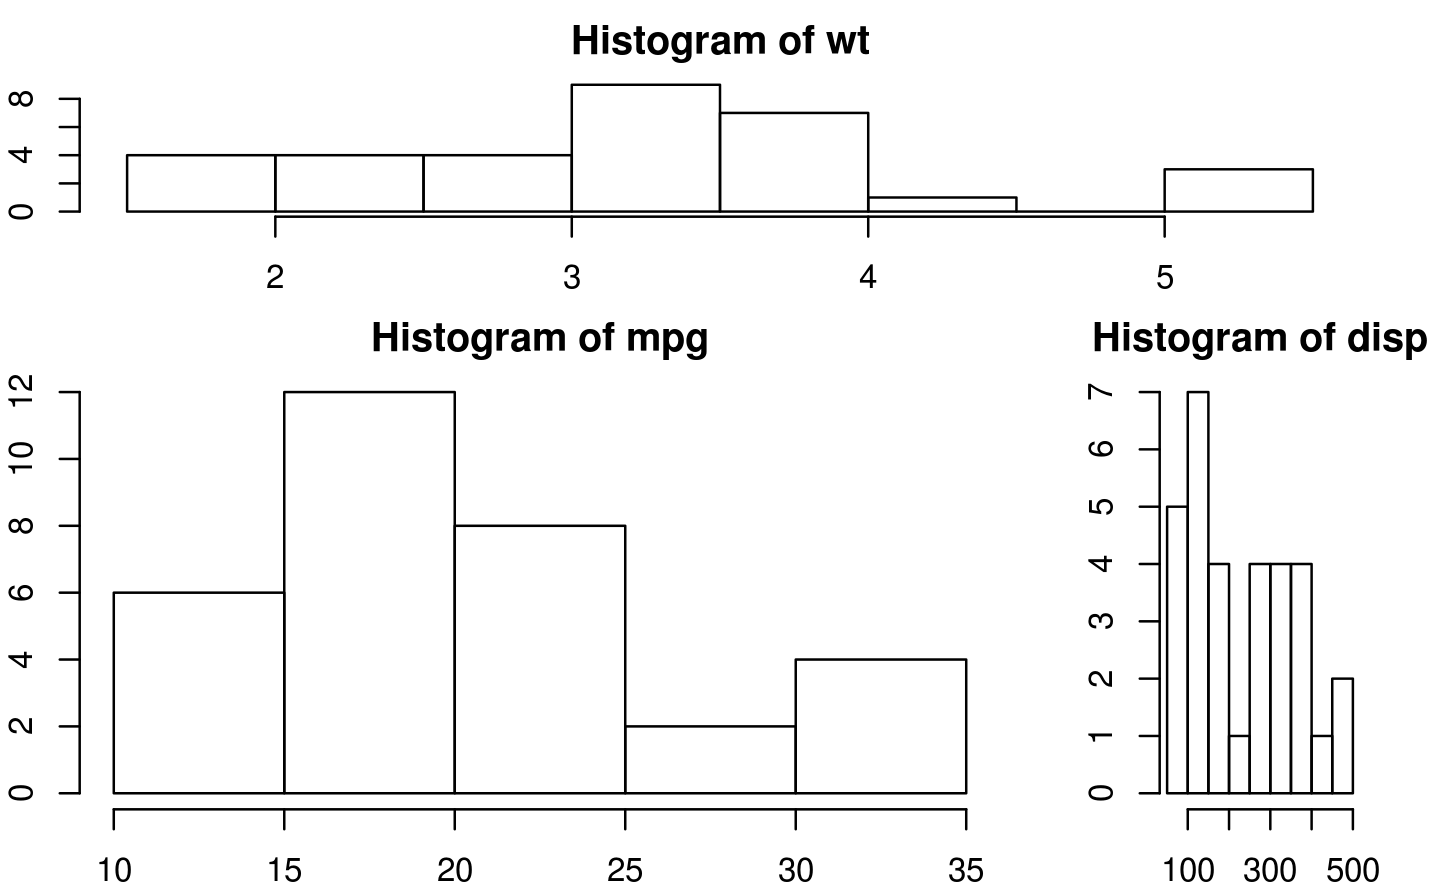
\includegraphics[width=0.7\linewidth]{rmi_copy_test_files/figure-latex/unnamed-chunk-370-1} \end{center}

multiplot layout with fine control click to view

See help(layout) for more details.

Creating a figure arrangement with fine control In the following
example, two box plots are added to scatterplot to create an enhanced
graph.

\begin{Shaded}
\begin{Highlighting}[]
\KeywordTok{par}\NormalTok{(}\DataTypeTok{mar =} \KeywordTok{rep}\NormalTok{(}\DecValTok{2}\NormalTok{, }\DecValTok{4}\NormalTok{)) }
\CommentTok{# Add boxplots to a scatterplot}
\KeywordTok{par}\NormalTok{(}\DataTypeTok{fig=}\KeywordTok{c}\NormalTok{(}\DecValTok{0}\NormalTok{,}\FloatTok{0.8}\NormalTok{,}\DecValTok{0}\NormalTok{,}\FloatTok{0.8}\NormalTok{), }\DataTypeTok{new=}\OtherTok{TRUE}\NormalTok{)}
\end{Highlighting}
\end{Shaded}

\begin{Shaded}
\begin{Highlighting}[]
\KeywordTok{plot}\NormalTok{(mtcars}\OperatorTok{$}\NormalTok{wt, mtcars}\OperatorTok{$}\NormalTok{mpg, }\DataTypeTok{xlab=}\StringTok{"Car Weight"}\NormalTok{,}
  \DataTypeTok{ylab=}\StringTok{"Miles Per Gallon"}\NormalTok{)}
\KeywordTok{par}\NormalTok{(}\DataTypeTok{fig=}\KeywordTok{c}\NormalTok{(}\DecValTok{0}\NormalTok{,}\FloatTok{0.8}\NormalTok{,}\FloatTok{0.55}\NormalTok{,}\DecValTok{1}\NormalTok{), }\DataTypeTok{new=}\OtherTok{TRUE}\NormalTok{)}
\KeywordTok{boxplot}\NormalTok{(mtcars}\OperatorTok{$}\NormalTok{wt, }\DataTypeTok{horizontal=}\OtherTok{TRUE}\NormalTok{, }\DataTypeTok{axes=}\OtherTok{FALSE}\NormalTok{)}
\KeywordTok{par}\NormalTok{(}\DataTypeTok{fig=}\KeywordTok{c}\NormalTok{(}\FloatTok{0.65}\NormalTok{,}\DecValTok{1}\NormalTok{,}\DecValTok{0}\NormalTok{,}\FloatTok{0.8}\NormalTok{),}\DataTypeTok{new=}\OtherTok{TRUE}\NormalTok{)}
\KeywordTok{boxplot}\NormalTok{(mtcars}\OperatorTok{$}\NormalTok{mpg, }\DataTypeTok{axes=}\OtherTok{FALSE}\NormalTok{)}
\KeywordTok{mtext}\NormalTok{(}\StringTok{"Enhanced Scatterplot"}\NormalTok{, }\DataTypeTok{side=}\DecValTok{3}\NormalTok{, }\DataTypeTok{outer=}\OtherTok{TRUE}\NormalTok{, }\DataTypeTok{line=}\OperatorTok{-}\DecValTok{3}\NormalTok{)}
\end{Highlighting}
\end{Shaded}

\begin{center}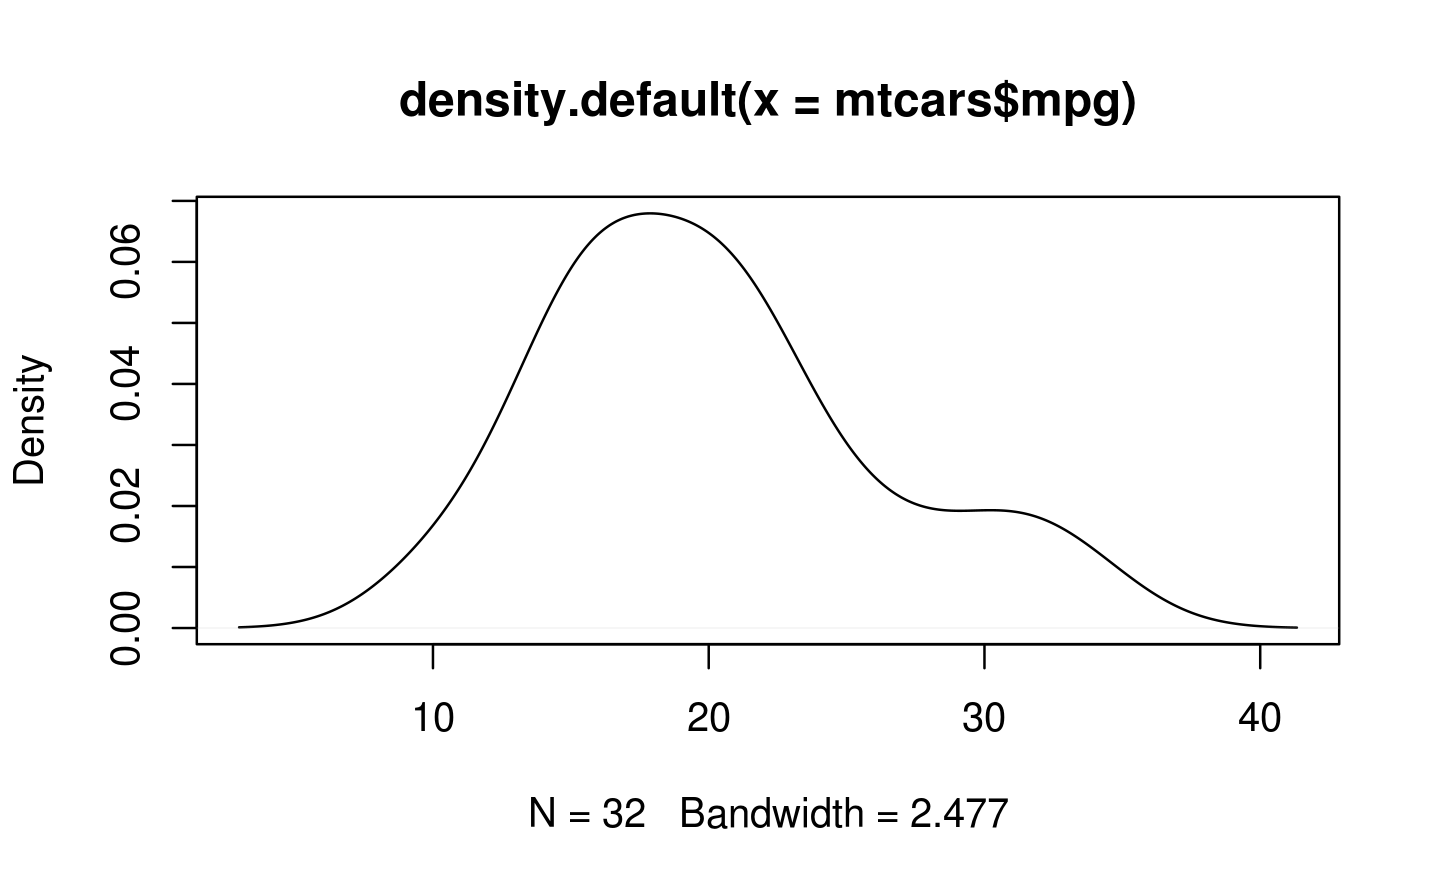
\includegraphics[width=0.7\linewidth]{rmi_copy_test_files/figure-latex/unnamed-chunk-371-1} \end{center}

To understand this graph, think of the full graph area as going from
(0,0) in the lower left corner to (1,1) in the upper right corner. The
format of the fig= parameter is a numerical vector of the form c(x1, x2,
y1, y2). The first fig= sets up the scatterplot going from 0 to 0.8 on
the x axis and 0 to 0.8 on the y axis. The top boxplot goes from 0 to
0.8 on the x axis and 0.55 to 1 on the y axis. I chose 0.55 rather than
0.8 so that the top figure will be pulled closer to the scatter plot.
The right hand boxplot goes from 0.65 to 1 on the x axis and 0 to 0.8 on
the y axis. Again, I chose a value to pull the right hand boxplot closer
to the scatterplot. You have to experiment to get it just right.

fig= starts a new plot, so to add to an existing plot use new=TRUE.

You can use this to combine several plots in any arrangement into one
graph.

\section{Add texts within the graph}\label{add-texts-within-the-graph}

The text() function can be used to draw text inside the plotting area. A
simplified format of the function is :

text(x, y, labels) x and y: 文字座標; labels: 例如 ``a label''

範例 :

\begin{Shaded}
\begin{Highlighting}[]
\NormalTok{d<-}\KeywordTok{head}\NormalTok{(mtcars)}
\KeywordTok{plot}\NormalTok{(d[,}\StringTok{'wt'}\NormalTok{], d[,}\StringTok{'mpg'}\NormalTok{], }
     \DataTypeTok{main=}\StringTok{"Milage vs. Car Weight}\CharTok{\textbackslash{}n}\StringTok{~~~~~~~~~~~~~~~~~~~"}\NormalTok{,}
      \DataTypeTok{xlab=}\StringTok{"Weight"}\NormalTok{, }\DataTypeTok{ylab=}\StringTok{"Miles/(US) gallon"}\NormalTok{,}
      \DataTypeTok{pch=}\DecValTok{19}\NormalTok{, }\DataTypeTok{col=}\StringTok{"darkgreen"}\NormalTok{)}
\KeywordTok{text}\NormalTok{(d[,}\StringTok{'wt'}\NormalTok{], d[,}\StringTok{'mpg'}\NormalTok{],  }\KeywordTok{row.names}\NormalTok{(d),     }\DataTypeTok{cex=}\FloatTok{0.65}\NormalTok{,}\DataTypeTok{pos=}\DecValTok{3}\NormalTok{,}\DataTypeTok{col=}\StringTok{"red"}\NormalTok{) }
\end{Highlighting}
\end{Shaded}

\begin{center}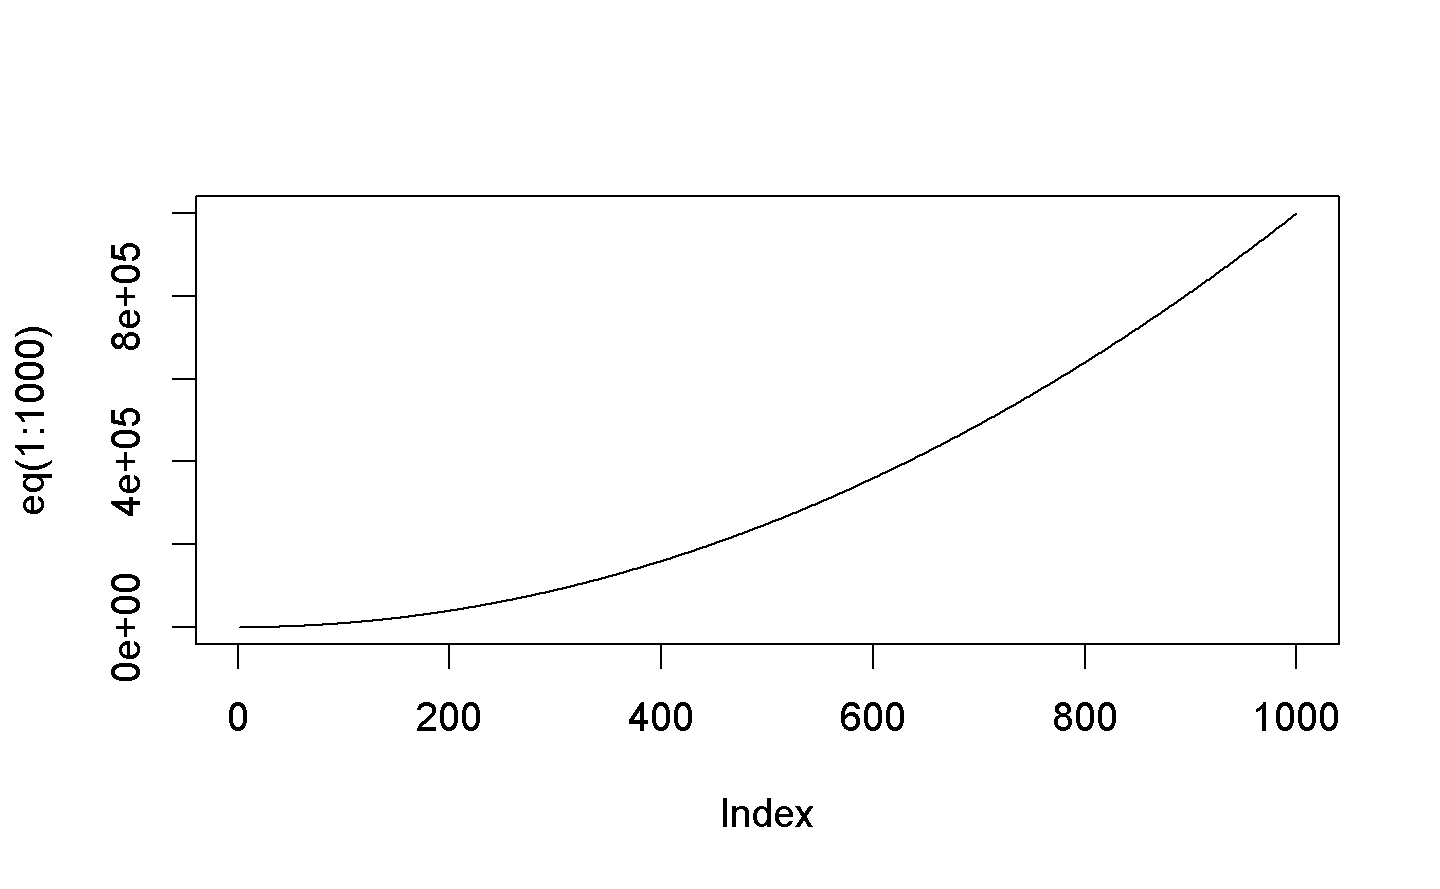
\includegraphics[width=0.7\linewidth]{rmi_copy_test_files/figure-latex/unnamed-chunk-374-1} \end{center}

\subsection{Add text in the margins of the
graph}\label{add-text-in-the-margins-of-the-graph}

在圖形周圍給文字:

mtext(text, side=3) text : 例如``a label'' side : 哪一側 :\\
順時針 1: 下 2: 左 3: 上 4: 又

範例 :

\begin{Shaded}
\begin{Highlighting}[]
\KeywordTok{plot}\NormalTok{(}\DecValTok{1}\OperatorTok{:}\DecValTok{10}\NormalTok{, }\DecValTok{1}\OperatorTok{:}\DecValTok{10}\NormalTok{, }
     \DataTypeTok{main=}\StringTok{"mtext(...) examples}\CharTok{\textbackslash{}n}\StringTok{~~~~~~~~~~~"}\NormalTok{)}
\KeywordTok{mtext}\NormalTok{(}\StringTok{"Magic function"}\NormalTok{, }\DataTypeTok{side=}\DecValTok{3}\NormalTok{)}
\end{Highlighting}
\end{Shaded}

\begin{center}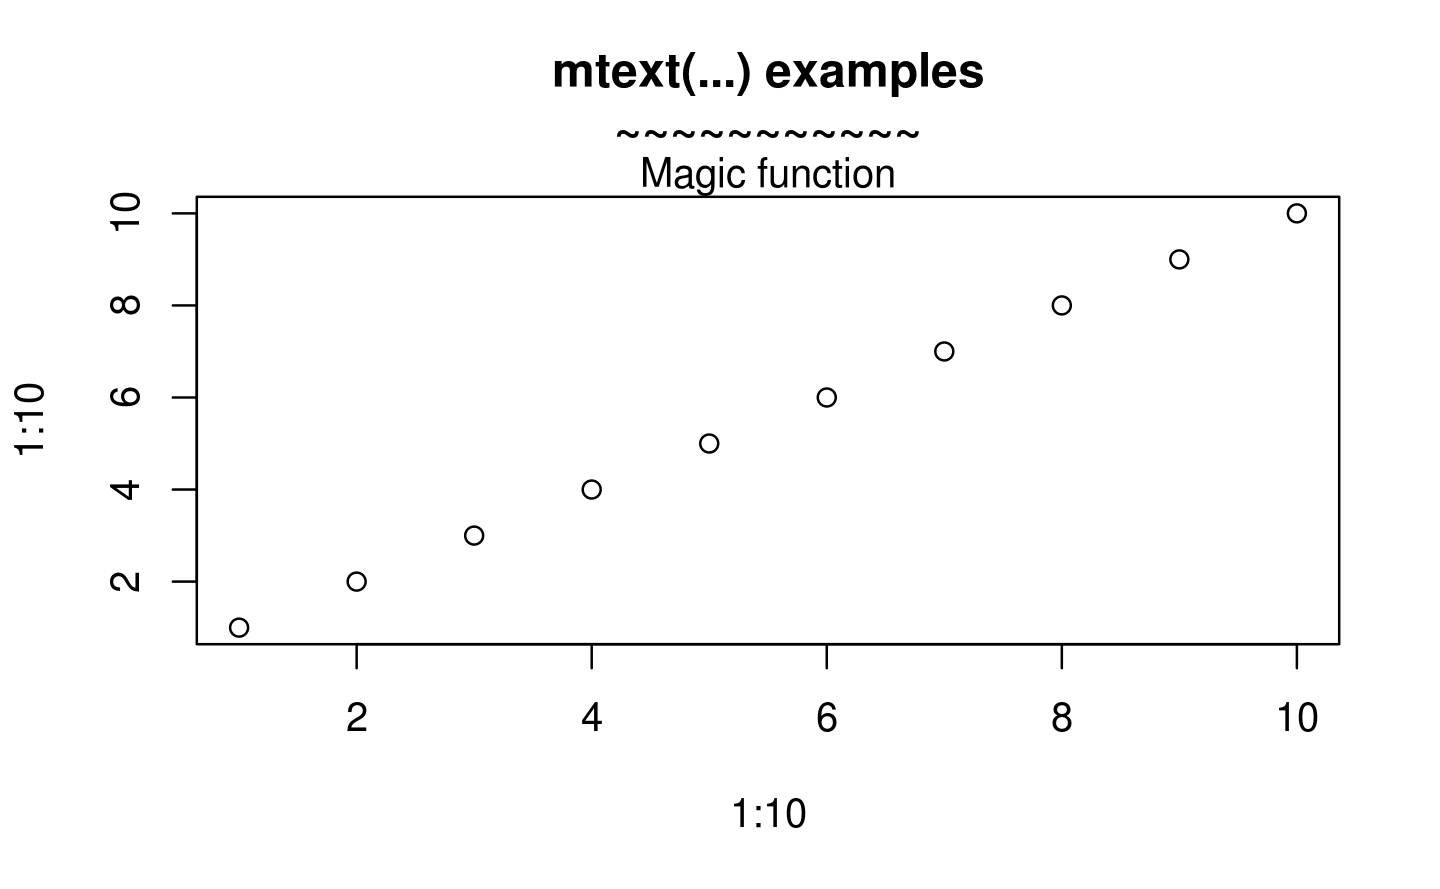
\includegraphics[width=0.7\linewidth]{rmi_copy_test_files/figure-latex/unnamed-chunk-375-1} \end{center}

\subsection{Add mathematical annotation to a
plot}\label{add-mathematical-annotation-to-a-plot}

\begin{Shaded}
\begin{Highlighting}[]
\KeywordTok{plot}\NormalTok{(}\DecValTok{1}\OperatorTok{:}\DecValTok{10}\NormalTok{, }\DecValTok{1}\OperatorTok{:}\DecValTok{10}\NormalTok{, }
     \DataTypeTok{main=}\StringTok{"text(...) examples}\CharTok{\textbackslash{}n}\StringTok{~~~~~~~~~~~"}\NormalTok{)}
\KeywordTok{text}\NormalTok{(}\DecValTok{4}\NormalTok{, }\DecValTok{9}\NormalTok{, }\KeywordTok{expression}\NormalTok{(}\KeywordTok{hat}\NormalTok{(beta) }\OperatorTok{==}\StringTok{ }\NormalTok{(X}\OperatorTok{^}\NormalTok{t }\OperatorTok{*}\StringTok{ }\NormalTok{X)}\OperatorTok{^}\NormalTok{\{}\OperatorTok{-}\DecValTok{1}\NormalTok{\} }\OperatorTok{*}\StringTok{ }\NormalTok{X}\OperatorTok{^}\NormalTok{t }\OperatorTok{*}\StringTok{ }\NormalTok{y))}
\KeywordTok{text}\NormalTok{(}\DecValTok{7}\NormalTok{, }\DecValTok{4}\NormalTok{, }\KeywordTok{expression}\NormalTok{(}\KeywordTok{bar}\NormalTok{(x) }\OperatorTok{==}\StringTok{ }\KeywordTok{sum}\NormalTok{(}\KeywordTok{frac}\NormalTok{(x[i], n), i}\OperatorTok{==}\DecValTok{1}\NormalTok{, n)))}
\end{Highlighting}
\end{Shaded}

\begin{center}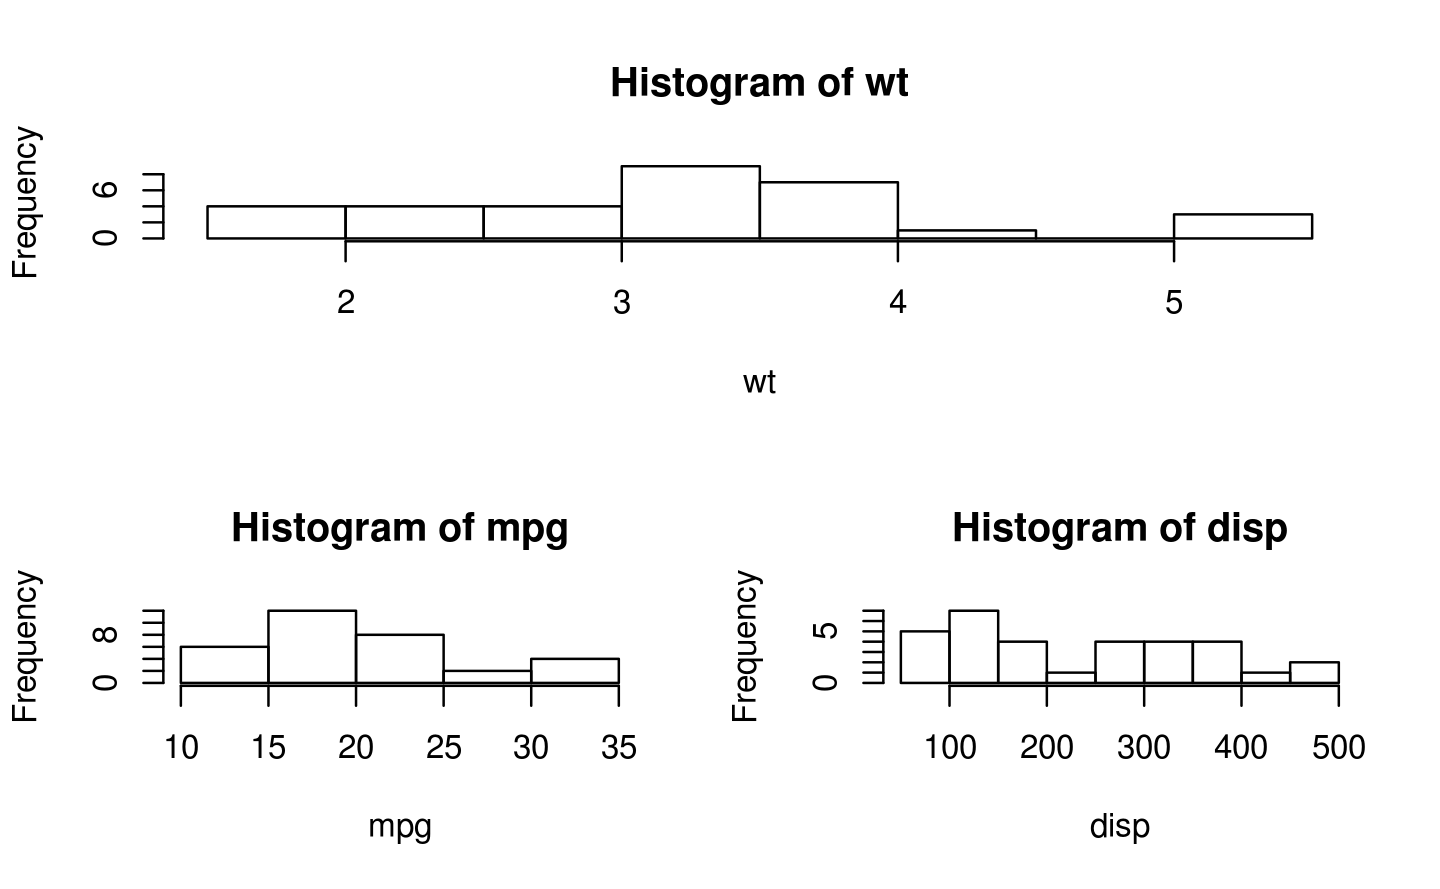
\includegraphics[width=0.7\linewidth]{rmi_copy_test_files/figure-latex/unnamed-chunk-376-1} \end{center}

\section{函數畫圖}

\begin{Shaded}
\begin{Highlighting}[]
\NormalTok{eq =}\StringTok{ }\ControlFlowTok{function}\NormalTok{(x)\{x}\OperatorTok{*}\NormalTok{x\}}
\KeywordTok{plot}\NormalTok{(}\KeywordTok{eq}\NormalTok{(}\DecValTok{1}\OperatorTok{:}\DecValTok{1000}\NormalTok{), }\DataTypeTok{type=}\StringTok{'l'}\NormalTok{)}
\end{Highlighting}
\end{Shaded}

\begin{center}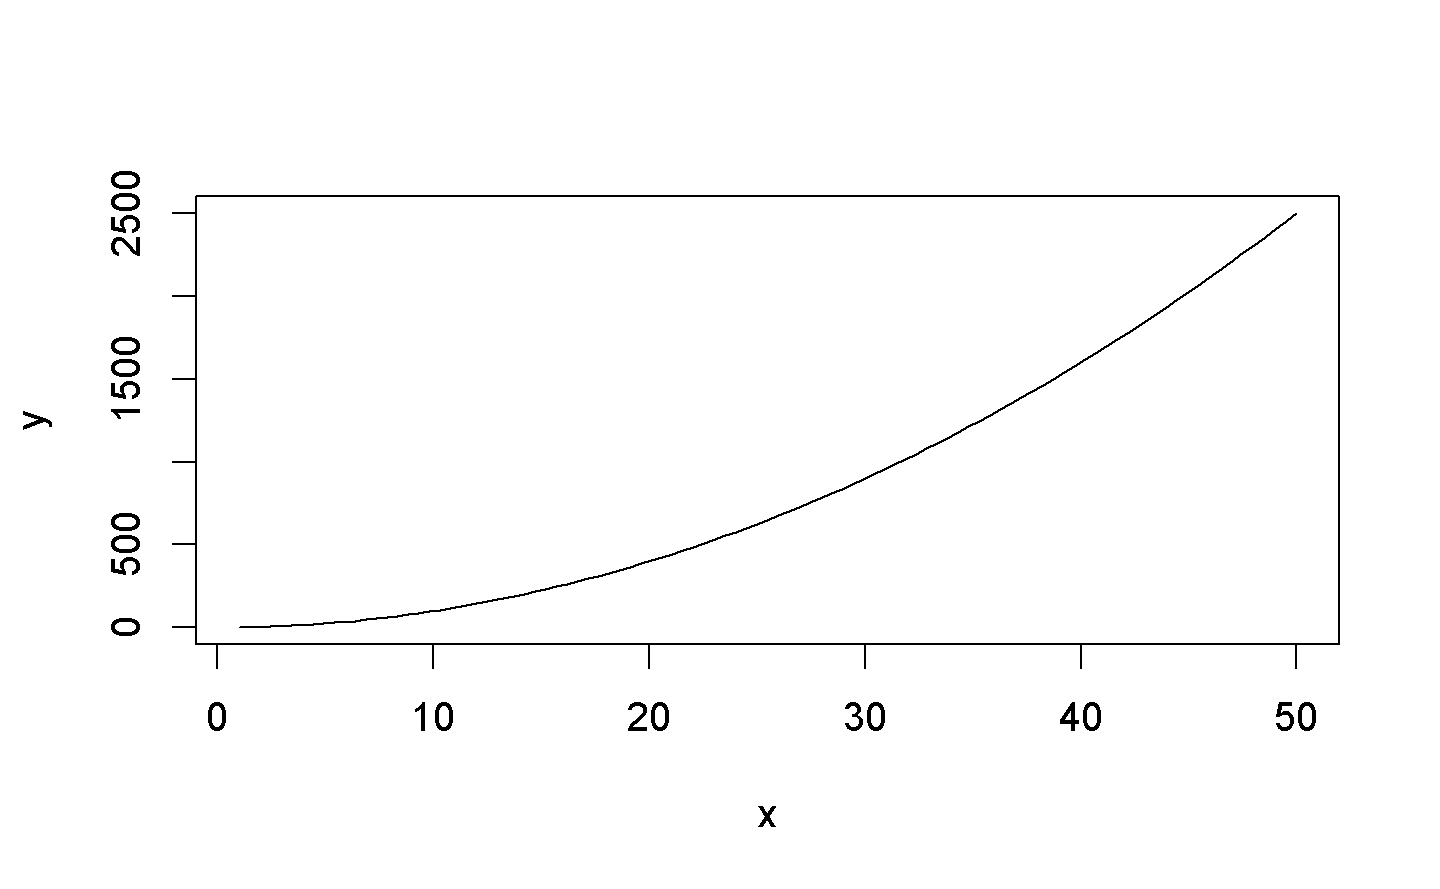
\includegraphics[width=0.7\linewidth]{rmi_copy_test_files/figure-latex/unnamed-chunk-377-1} \end{center}

問題是如果x座標的增加不是1單位?

\begin{Shaded}
\begin{Highlighting}[]
\NormalTok{x<-}\KeywordTok{seq}\NormalTok{(}\DecValTok{1}\NormalTok{,}\DecValTok{10}\NormalTok{,}\FloatTok{0.1}\NormalTok{)}
\NormalTok{y<-}\KeywordTok{exp}\NormalTok{(x)}
\NormalTok{x<-y}

\NormalTok{eq =}\StringTok{ }\ControlFlowTok{function}\NormalTok{(x)\{x}\OperatorTok{*}\NormalTok{x\}}
\KeywordTok{plot}\NormalTok{(x,}\KeywordTok{eq}\NormalTok{(x), }\DataTypeTok{type=}\StringTok{'l'}\NormalTok{)}
\end{Highlighting}
\end{Shaded}

\begin{center}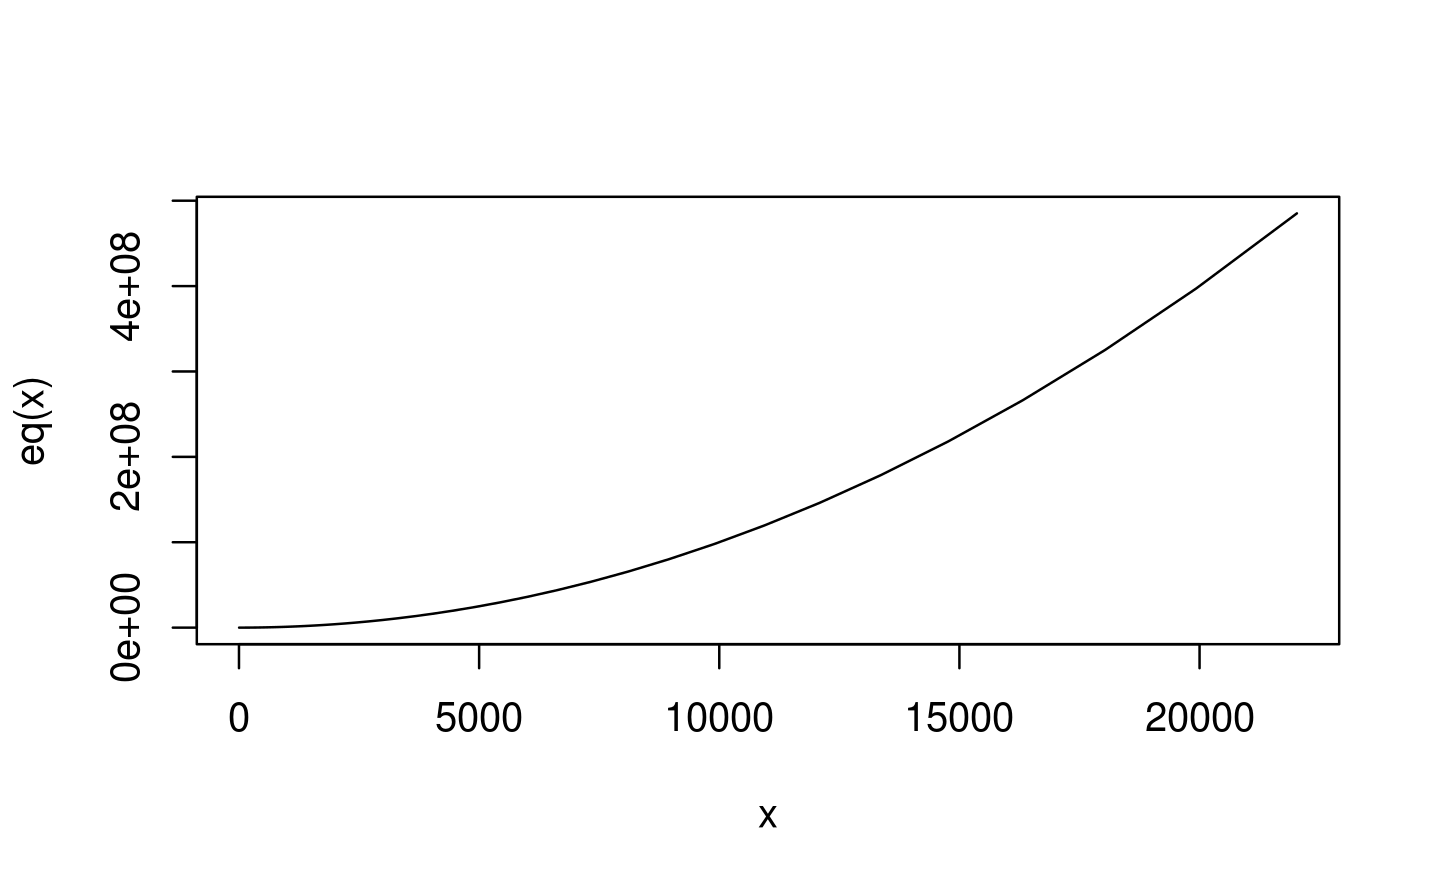
\includegraphics[width=0.7\linewidth]{rmi_copy_test_files/figure-latex/unnamed-chunk-378-1} \end{center}

\begin{Shaded}
\begin{Highlighting}[]
\NormalTok{eq =}\StringTok{ }\ControlFlowTok{function}\NormalTok{(x)\{x}\OperatorTok{*}\NormalTok{x\}}
\KeywordTok{curve}\NormalTok{(eq, }\DataTypeTok{from=}\DecValTok{1}\NormalTok{, }\DataTypeTok{to=}\DecValTok{50}\NormalTok{, }\DataTypeTok{xlab=}\StringTok{"x"}\NormalTok{, }\DataTypeTok{ylab=}\StringTok{"y"}\NormalTok{)}
\end{Highlighting}
\end{Shaded}

\begin{center}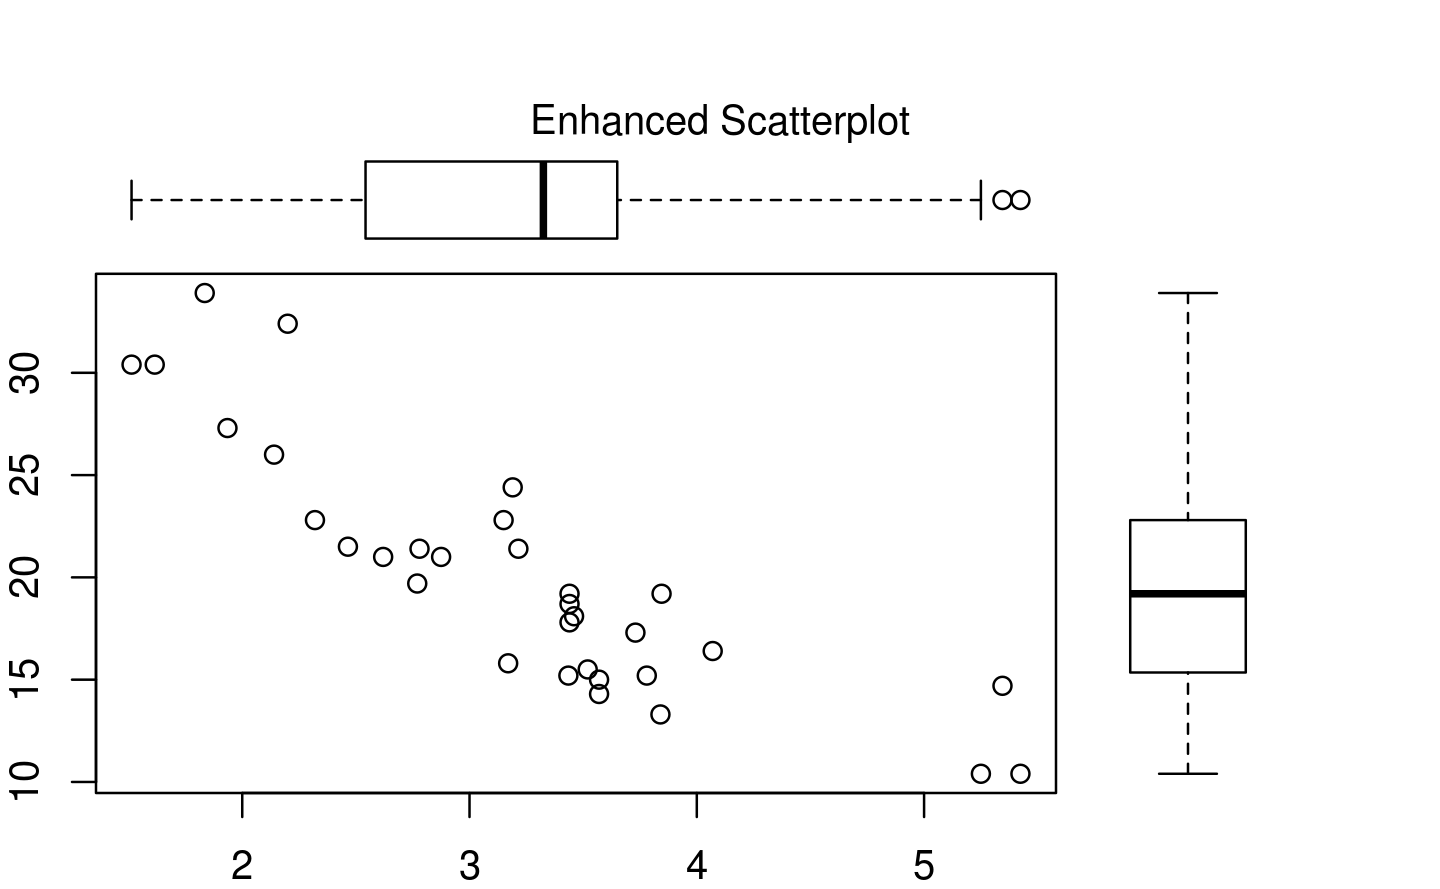
\includegraphics[width=0.7\linewidth]{rmi_copy_test_files/figure-latex/unnamed-chunk-379-1} \end{center}

問題:解釋為何錯誤

\begin{Shaded}
\begin{Highlighting}[]
\NormalTok{eq =}\StringTok{ }\ControlFlowTok{function}\NormalTok{(x)\{x}\OperatorTok{*}\NormalTok{x\}}
\NormalTok{y<-}\KeywordTok{eq}\NormalTok{(}\DecValTok{1}\OperatorTok{:}\DecValTok{50}\NormalTok{)}
\KeywordTok{curve}\NormalTok{(y, }\DataTypeTok{xlab=}\StringTok{"x"}\NormalTok{, }\DataTypeTok{ylab=}\StringTok{"y"}\NormalTok{)}
\end{Highlighting}
\end{Shaded}

問題:如何修正下面的錯誤?

\begin{Shaded}
\begin{Highlighting}[]
\NormalTok{eq =}\StringTok{ }\ControlFlowTok{function}\NormalTok{(x)\{x}\OperatorTok{*}\NormalTok{x\}}
\NormalTok{z<-}\DecValTok{1}\OperatorTok{:}\DecValTok{50}

\KeywordTok{curve}\NormalTok{(}\KeywordTok{eq}\NormalTok{(z), }\DataTypeTok{xlab=}\StringTok{"x"}\NormalTok{, }\DataTypeTok{ylab=}\StringTok{"y"}\NormalTok{)}
\end{Highlighting}
\end{Shaded}

solution:

\chapter{Sample and Distribution 01}\label{sample-and-distribution-01}

\section{ 隨機抽樣}

函數sample(x,n,replace=FALSE ). 其中x為要抽取的向量, n為樣本容量.
replace 預設為false

\begin{enumerate}
\def\labelenumi{\arabic{enumi}.}
\tightlist
\item
  no replacement, 等機率:
\end{enumerate}

例如從52張撲克牌中抽取5張:

\begin{Shaded}
\begin{Highlighting}[]
\KeywordTok{sample}\NormalTok{(}\DecValTok{1}\OperatorTok{:}\DecValTok{52}\NormalTok{, }\DecValTok{5}\NormalTok{)}
\end{Highlighting}
\end{Shaded}

\begin{enumerate}
\def\labelenumi{\arabic{enumi}.}
\setcounter{enumi}{1}
\tightlist
\item
  replacement: 例如拋一枚均勻的硬幣10次
\end{enumerate}

\begin{Shaded}
\begin{Highlighting}[]
 \KeywordTok{sample}\NormalTok{(}\KeywordTok{c}\NormalTok{(}\StringTok{"H"}\NormalTok{, }\StringTok{"T"}\NormalTok{), }\DecValTok{10}\NormalTok{, }\DataTypeTok{replace=}\NormalTok{T)}
\end{Highlighting}
\end{Shaded}

練習:一棵骰子擲10次可表示為:

\begin{enumerate}
\def\labelenumi{\arabic{enumi})}
\setcounter{enumi}{2}
\tightlist
\item
  不等可能的隨機抽樣: sample(x, n, replace=TRUE, prob=y)
  prob=y指定x中元素出現的概率, 向量y與x等長度.
  例如一娃娃機取出成功的概率為0.6, 那麼10次的試驗為:
\end{enumerate}

\begin{Shaded}
\begin{Highlighting}[]
\KeywordTok{sample}\NormalTok{(}\KeywordTok{c}\NormalTok{(}\StringTok{"sucess"}\NormalTok{, }\StringTok{"fail"}\NormalTok{), }\DecValTok{10}\NormalTok{, }\DataTypeTok{replace=}\NormalTok{T, }\DataTypeTok{prob=}\KeywordTok{c}\NormalTok{(}\FloatTok{0.6}\NormalTok{,}\FloatTok{0.4}\NormalTok{))}
\end{Highlighting}
\end{Shaded}

\section{排列組合與概率的計算}

例 從一副52張撲克中取4張, 求以下事件的概率:\\
1. 抽取的4張依次為紅心A,方塊A,黑桃A和梅花A的概率;\\
2. 一次抽取4張為紅心A,方塊A,黑桃A和梅花A的概率.

his summation expression \(\sum_{i=1}^n X_i\) appears inline.

解\\
1) 抽取的4張是有次序的, 因此使用排列來求解. 所求的事件(記為A)概率為
\(P(A)=\frac{1}{52 \times 51 \times 50 \times 49}\) 利用R函數

\begin{Shaded}
\begin{Highlighting}[]
\DecValTok{1}\OperatorTok{/}\KeywordTok{prod}\NormalTok{(}\DecValTok{52}\OperatorTok{:}\DecValTok{49}\NormalTok{)}
\end{Highlighting}
\end{Shaded}

\begin{enumerate}
\def\labelenumi{\arabic{enumi}.}
\setcounter{enumi}{1}
\tightlist
\item
  沒有次序的, 可以使用組合數來求解.
\end{enumerate}

\[ P(B)=\frac{1}{(52,4)} \]

其中 \((n,m)=\frac{n!}{m!(n-m)!}\),可以利用函數choose(),例如

\begin{Shaded}
\begin{Highlighting}[]
\DecValTok{1}\OperatorTok{/}\KeywordTok{choose}\NormalTok{(}\DecValTok{52}\NormalTok{,}\DecValTok{4}\NormalTok{)}
\end{Highlighting}
\end{Shaded}

\section{distribution}\label{distribution}

標準表格上下沒有線條,左右有

\begin{longtable}[]{@{}lll@{}}
\toprule
名稱 & R函數 & 選項\tabularnewline
\midrule
\endhead
beta & beta & shape1, shape2\tabularnewline
binomial & binom & size, prob\tabularnewline
Cauchy & cauchy & location=0, scale=1\tabularnewline
chi-sqaured (\(\chi^2\)) & chisq & df, ncp\tabularnewline
exponential & exp & rate\tabularnewline
Fisher (F) & f & df1, df2, ncp\tabularnewline
gamma & gamma & shape, scale=1\tabularnewline
geometric & geom & prob\tabularnewline
hypergeometric & hyper & m, n, k\tabularnewline
lognormal & lnorm & meanlog=0, sdlog=1\tabularnewline
logistic & logis & location=0, scale=1\tabularnewline
multinomial & multinom & size, prob\tabularnewline
normal & norm & mean=0, sd=1\tabularnewline
negative binomial & nbinom & size, prob\tabularnewline
Poisson & pois & lambda\tabularnewline
Student's (t) & t & df\tabularnewline
uniform & unif & min=0, max=1\tabularnewline
Weibull & weibull & shape, scale=1\tabularnewline
Wilcoxon's statistics & wilcox & m, n\tabularnewline
& signrank & n\tabularnewline
\bottomrule
\end{longtable}

對於所給的分佈名稱,有四類。

以func為例, 四類函數的對應為:\\
1. 「d」概率密度函數: dfunc(x, p1, p2, \ldots{}), x為數值向量;\\
1. 「p」(累積)分佈函數: pfunc(q, p1, p2, \ldots{}), q為數值向量;\\
1. 「q」分位數函數: qfunc(p, p1, p2, \ldots{}), p為由概率構成的向量;\\
1. 「r」隨機數函數: rfunc(n, p1, p2, \ldots{}), n為生成數據的個數

這四類函數的第一個參數是有規律的:
形為dfunc的函數為x,pfunc的函數為q,qfunc的函數為p,rfunc的函數為n

note: (但rhyper和rwilcox是特例,他們的第一個參數為nn).
非中心參數(non-centrality parameter)僅對CDF和 少數其它幾個函數有效.

\[ \frac{{\sum\limits_{i = 1}^n {{x_i} - n\mu } }}{{\sqrt {n{\sigma ^2}} }} \sim  N(0,1) \]

\[ \bar X = \frac{{\sum_{i = 1}^n {{x_i} } }}{n} \sim  N(\mu, \sigma^2/n) \]

uniform a\textasciitilde{}b \[\mu = (a+b)/2\]
\[\sigma^2=\frac{(b-a)^2}{12} \] data的每一個ROW有sample size
(=i=column)\\
共1000次(=N=row)

\begin{Shaded}
\begin{Highlighting}[]
\NormalTok{N=}\DecValTok{1000} 
\NormalTok{i=}\DecValTok{3} \CommentTok{#sample size}
\NormalTok{mu=}\FloatTok{0.5}
\NormalTok{sigma=}\DecValTok{1}\OperatorTok{/}\KeywordTok{sqrt}\NormalTok{(}\DecValTok{12}\NormalTok{)}
\NormalTok{data<-}\KeywordTok{matrix}\NormalTok{(}\KeywordTok{runif}\NormalTok{(i}\OperatorTok{*}\NormalTok{N),}\DataTypeTok{ncol=}\NormalTok{i)}
\NormalTok{rs<-}\KeywordTok{rowSums}\NormalTok{(data)}
\NormalTok{rs<-rs}\OperatorTok{/}\NormalTok{i}
\NormalTok{z<-(rs}\OperatorTok{-}\NormalTok{mu)}\OperatorTok{/}\NormalTok{(sigma}\OperatorTok{/}\KeywordTok{sqrt}\NormalTok{(i))}
\KeywordTok{hist}\NormalTok{(z)}
\KeywordTok{lines}\NormalTok{(}\KeywordTok{density}\NormalTok{(z), }\DataTypeTok{col =} \StringTok{'red'}\NormalTok{, }\DataTypeTok{lwd =} \DecValTok{3}\NormalTok{)}
\NormalTok{x<-z}
\KeywordTok{curve}\NormalTok{(}\KeywordTok{dnorm}\NormalTok{(x), }\DataTypeTok{col =} \StringTok{'blue'}\NormalTok{, }\DataTypeTok{lwd =} \DecValTok{3}\NormalTok{, }\DataTypeTok{lty =} \DecValTok{3}\NormalTok{, }\DataTypeTok{add =}\NormalTok{ T)}
\KeywordTok{rug}\NormalTok{(}\KeywordTok{sample}\NormalTok{(z,}\DecValTok{100}\NormalTok{))}
\end{Highlighting}
\end{Shaded}

\begin{center}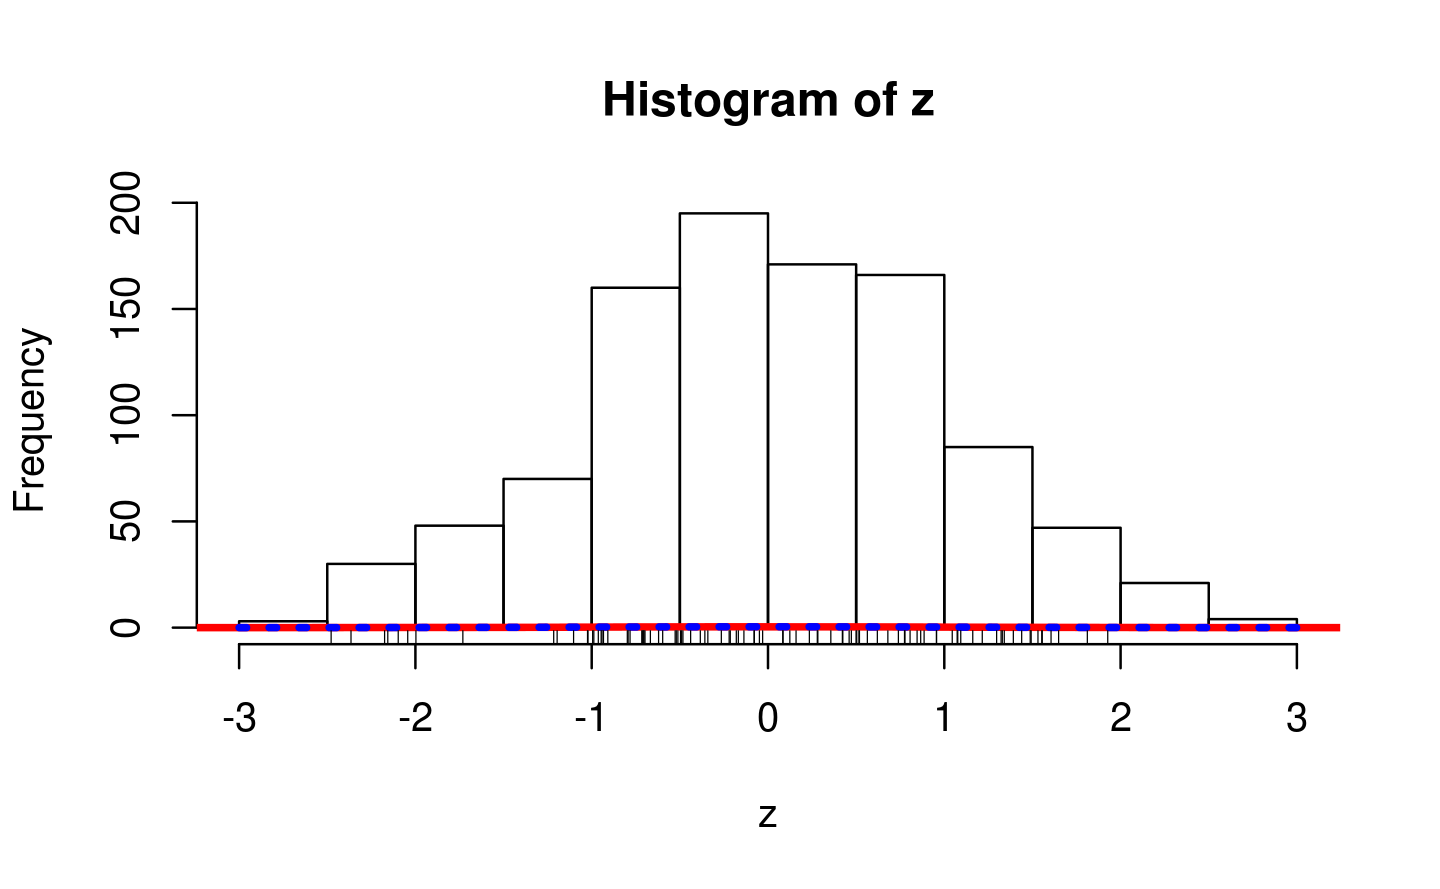
\includegraphics[width=0.7\linewidth]{rmi_copy_test_files/figure-latex/unnamed-chunk-391-1} \end{center}

\begin{Shaded}
\begin{Highlighting}[]
\NormalTok{limite.central <-}
\StringTok{  }\ControlFlowTok{function}\NormalTok{ (}\DataTypeTok{r =}\NormalTok{ runif, }\DataTypeTok{distpar =} \KeywordTok{c}\NormalTok{(}\DecValTok{0}\NormalTok{, }\DecValTok{1}\NormalTok{), }\DataTypeTok{m =}\NormalTok{ .}\DecValTok{5}\NormalTok{, }\DataTypeTok{s =} \DecValTok{1} \OperatorTok{/}\StringTok{ }\KeywordTok{sqrt}\NormalTok{(}\DecValTok{12}\NormalTok{), }\DataTypeTok{n =} \KeywordTok{c}\NormalTok{(}\DecValTok{1}\NormalTok{, }\DecValTok{3}\NormalTok{, }\DecValTok{10}\NormalTok{, }\DecValTok{30}\NormalTok{), }\DataTypeTok{N =} \DecValTok{1000}\NormalTok{) \{}
    \ControlFlowTok{for}\NormalTok{ (i }\ControlFlowTok{in}\NormalTok{ n) \{}
      \ControlFlowTok{if}\NormalTok{ (}\KeywordTok{length}\NormalTok{(distpar) }\OperatorTok{==}\StringTok{ }\DecValTok{2}\NormalTok{) \{}
\NormalTok{        x <-}\KeywordTok{matrix}\NormalTok{(}\KeywordTok{r}\NormalTok{(i }\OperatorTok{*}\StringTok{ }\NormalTok{N, distpar[}\DecValTok{1}\NormalTok{], distpar[}\DecValTok{2}\NormalTok{]), }\DataTypeTok{nc =}\NormalTok{ i)}
\NormalTok{      \} }\ControlFlowTok{else}\NormalTok{ \{}
\NormalTok{        x <-}\KeywordTok{matrix}\NormalTok{(}\KeywordTok{r}\NormalTok{(i }\OperatorTok{*}\StringTok{ }\NormalTok{N, distpar), }\DataTypeTok{nc =}\NormalTok{ i)}
\NormalTok{      \}}
\NormalTok{      x <-(}\KeywordTok{apply}\NormalTok{(x, }\DecValTok{1}\NormalTok{, sum) }\OperatorTok{-}\StringTok{ }\NormalTok{i }\OperatorTok{*}\StringTok{ }\NormalTok{m) }\OperatorTok{/}\StringTok{ }\NormalTok{(}\KeywordTok{sqrt}\NormalTok{(i) }\OperatorTok{*}\StringTok{ }\NormalTok{s)}
      \KeywordTok{hist}\NormalTok{(x, }\DataTypeTok{col =} \StringTok{'light blue'}\NormalTok{, }\DataTypeTok{probability =}\NormalTok{ T, }\DataTypeTok{main =} \KeywordTok{paste}\NormalTok{(}\StringTok{"n="}\NormalTok{, i),}
        \DataTypeTok{ylim =} \KeywordTok{c}\NormalTok{(}\DecValTok{0}\NormalTok{, }\KeywordTok{max}\NormalTok{(.}\DecValTok{4}\NormalTok{, }\KeywordTok{density}\NormalTok{(x) }\OperatorTok{$}\NormalTok{y)))}
      \KeywordTok{lines}\NormalTok{(}\KeywordTok{density}\NormalTok{(x), }\DataTypeTok{col =} \StringTok{'red'}\NormalTok{, }\DataTypeTok{lwd =} \DecValTok{3}\NormalTok{)}
      \KeywordTok{curve}\NormalTok{(}\KeywordTok{dnorm}\NormalTok{(x), }\DataTypeTok{col =} \StringTok{'blue'}\NormalTok{, }\DataTypeTok{lwd =} \DecValTok{3}\NormalTok{, }\DataTypeTok{lty =} \DecValTok{3}\NormalTok{, }\DataTypeTok{add =}\NormalTok{ T)}
      \ControlFlowTok{if}\NormalTok{ (N }\OperatorTok{>}\StringTok{ }\DecValTok{100}\NormalTok{) \{}
        \KeywordTok{rug}\NormalTok{(}\KeywordTok{sample}\NormalTok{(x, }\DecValTok{100}\NormalTok{))}
\NormalTok{      \} }\ControlFlowTok{else}\NormalTok{ \{}
        \KeywordTok{rug}\NormalTok{(x)}
\NormalTok{      \}}
\NormalTok{    \}}
\NormalTok{  \}}
\NormalTok{op <-}\StringTok{ }\KeywordTok{par}\NormalTok{(}\DataTypeTok{mfrow=}\KeywordTok{c}\NormalTok{(}\DecValTok{2}\NormalTok{,}\DecValTok{2}\NormalTok{))}
\KeywordTok{limite.central}\NormalTok{(rbinom, }\DataTypeTok{distpar=}\KeywordTok{c}\NormalTok{(}\DecValTok{10}\NormalTok{ ,}\FloatTok{0.1}\NormalTok{), }\DataTypeTok{m=}\DecValTok{1}\NormalTok{, }\DataTypeTok{s=}\FloatTok{0.9}\NormalTok{)}
\KeywordTok{par}\NormalTok{(op)}
\end{Highlighting}
\end{Shaded}

\begin{center}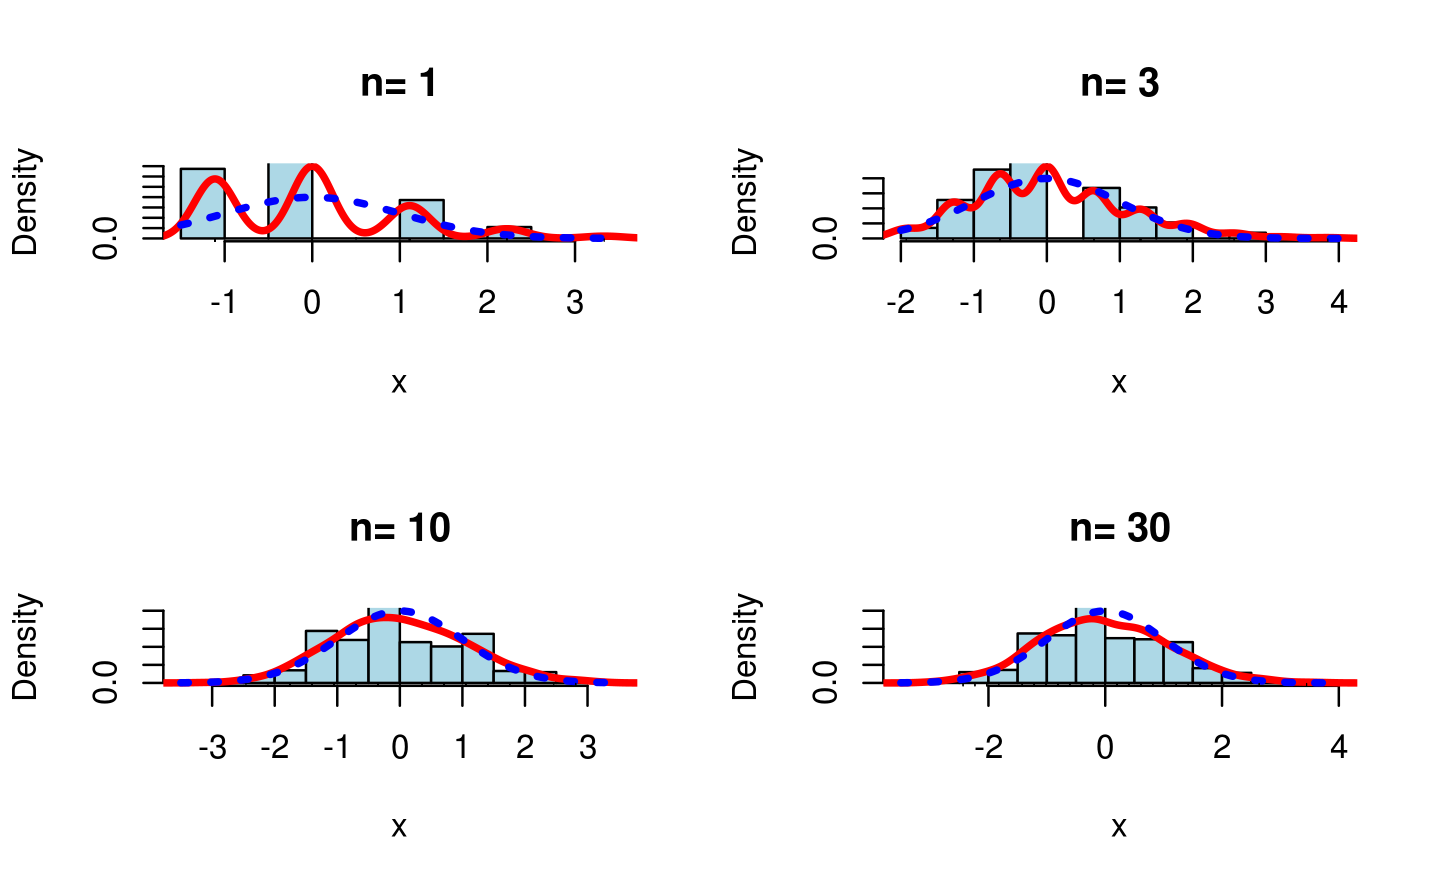
\includegraphics[width=0.7\linewidth]{rmi_copy_test_files/figure-latex/unnamed-chunk-392-1} \end{center}

\begin{itemize}
\tightlist
\item
  apply(x,1,sum) 第2個參數1表示row 方向,如果是2表示column 和matlab
  相反。
\end{itemize}

\begin{Shaded}
\begin{Highlighting}[]
\NormalTok{需要安裝babynames,ggplot2}
\end{Highlighting}
\end{Shaded}

\chapter{Tidy Basic 01}\label{tidy-basic-01}

\begin{Shaded}
\begin{Highlighting}[]
\KeywordTok{require}\NormalTok{(tidyr)}
\KeywordTok{require}\NormalTok{(dplyr) }\CommentTok{# data_frame}
\end{Highlighting}
\end{Shaded}

From \url{http://stackoverflow.com/questions/1181060}

\begin{Shaded}
\begin{Highlighting}[]
\NormalTok{stocks <-}\StringTok{ }\KeywordTok{data_frame}\NormalTok{(}
  \DataTypeTok{time =} \KeywordTok{as.Date}\NormalTok{(}\StringTok{'2009-01-01'}\NormalTok{) }\OperatorTok{+}\StringTok{ }\DecValTok{0}\OperatorTok{:}\DecValTok{9}\NormalTok{,}
  \DataTypeTok{X =} \KeywordTok{rnorm}\NormalTok{(}\DecValTok{10}\NormalTok{, }\DecValTok{0}\NormalTok{, }\DecValTok{1}\NormalTok{),}
  \DataTypeTok{Y =} \KeywordTok{rnorm}\NormalTok{(}\DecValTok{10}\NormalTok{, }\DecValTok{0}\NormalTok{, }\DecValTok{2}\NormalTok{),}
  \DataTypeTok{Z =} \KeywordTok{rnorm}\NormalTok{(}\DecValTok{10}\NormalTok{, }\DecValTok{0}\NormalTok{, }\DecValTok{4}\NormalTok{)}
\NormalTok{)}
\end{Highlighting}
\end{Shaded}

\begin{Shaded}
\begin{Highlighting}[]
\NormalTok{dset1 <-}\StringTok{ }\KeywordTok{head}\NormalTok{(stocks)}
\NormalTok{knitr}\OperatorTok{::}\KeywordTok{kable}\NormalTok{(dset1, }\DataTypeTok{format =} \StringTok{"html"}\NormalTok{)}
\end{Highlighting}
\end{Shaded}

time

X

Y

Z

2009-01-01

-1.400

-1.11

1.87

2009-01-02

0.255

1.26

1.45

2009-01-03

-2.437

4.13

-5.22

2009-01-04

-0.006

-3.26

2.95

2009-01-05

0.622

1.02

7.55

2009-01-06

1.148

-3.73

-0.39

\begin{Shaded}
\begin{Highlighting}[]
\KeywordTok{gather}\NormalTok{(stocks, stock, price, }\OperatorTok{-}\NormalTok{time)}
\end{Highlighting}
\end{Shaded}

\begin{Shaded}
\begin{Highlighting}[]
\NormalTok{stocks }\OperatorTok\StringTok{ }\KeywordTok{gather}\NormalTok{(stock, price, }\OperatorTok{-}\NormalTok{time)}
\end{Highlighting}
\end{Shaded}

\begin{Shaded}
\begin{Highlighting}[]
\NormalTok{dset1 <-}\StringTok{ }\KeywordTok{head}\NormalTok{(stocks)}
\NormalTok{knitr}\OperatorTok{::}\KeywordTok{kable}\NormalTok{(dset1, }\DataTypeTok{format =} \StringTok{"html"}\NormalTok{)}
\end{Highlighting}
\end{Shaded}

time

X

Y

Z

2009-01-01

-1.400

-1.11

1.87

2009-01-02

0.255

1.26

1.45

2009-01-03

-2.437

4.13

-5.22

2009-01-04

-0.006

-3.26

2.95

2009-01-05

0.622

1.02

7.55

2009-01-06

1.148

-3.73

-0.39

設定css

\begin{Shaded}
\begin{Highlighting}[]
\KeywordTok{writeLines}\NormalTok{(}\StringTok{"td, th \{ padding : 6px \} th \{ background-color : brown ; color : white; border : 1px solid white; \} td \{ color : brown ; border : 1px solid brown \}"}\NormalTok{, }\DataTypeTok{con =} \StringTok{"tableStyle.css"}\NormalTok{)}
\end{Highlighting}
\end{Shaded}

\begin{Shaded}
\begin{Highlighting}[]
\NormalTok{stocks <-}\StringTok{ }\KeywordTok{data_frame}\NormalTok{(}
  \DataTypeTok{time =} \KeywordTok{as.Date}\NormalTok{(}\StringTok{'2009-01-01'}\NormalTok{) }\OperatorTok{+}\StringTok{ }\DecValTok{0}\OperatorTok{:}\DecValTok{9}\NormalTok{,}
  \DataTypeTok{X =} \KeywordTok{rnorm}\NormalTok{(}\DecValTok{10}\NormalTok{, }\DecValTok{0}\NormalTok{, }\DecValTok{1}\NormalTok{),}
  \DataTypeTok{Y =} \KeywordTok{rnorm}\NormalTok{(}\DecValTok{10}\NormalTok{, }\DecValTok{0}\NormalTok{, }\DecValTok{2}\NormalTok{),}
  \DataTypeTok{Z =} \KeywordTok{rnorm}\NormalTok{(}\DecValTok{10}\NormalTok{, }\DecValTok{0}\NormalTok{, }\DecValTok{4}\NormalTok{)}
\NormalTok{)}
\NormalTok{dset1 <-}\StringTok{ }\KeywordTok{head}\NormalTok{(stocks)}
\NormalTok{knitr}\OperatorTok{::}\KeywordTok{kable}\NormalTok{(dset1, }\DataTypeTok{format =} \StringTok{"html"}\NormalTok{)}
\end{Highlighting}
\end{Shaded}

time

X

Y

Z

2009-01-01

0.935

0.140

3.448

2009-01-02

0.176

-1.278

-0.973

2009-01-03

0.244

-0.100

-0.824

2009-01-04

1.624

-0.503

0.077

2009-01-05

0.112

0.890

0.118

2009-01-06

-0.134

5.511

2.199

\begin{Shaded}
\begin{Highlighting}[]
\NormalTok{demo<-}\KeywordTok{gather}\NormalTok{(stocks, stock, price, }\OperatorTok{-}\NormalTok{time)}

\NormalTok{dset1 <-}\StringTok{ }\KeywordTok{head}\NormalTok{(demo)}
\NormalTok{knitr}\OperatorTok{::}\KeywordTok{kable}\NormalTok{(dset1, }\DataTypeTok{format =} \StringTok{"html"}\NormalTok{)}
\end{Highlighting}
\end{Shaded}

time

stock

price

2009-01-01

X

0.935

2009-01-02

X

0.176

2009-01-03

X

0.244

2009-01-04

X

1.624

2009-01-05

X

0.112

2009-01-06

X

-0.134

\section{long and wide data}\label{long-and-wide-data}

\subsection{gather: wide to long}\label{gather-wide-to-long}

\begin{Shaded}
\begin{Highlighting}[]
\NormalTok{wide <-}\StringTok{ }\KeywordTok{data_frame}\NormalTok{(}
  \DataTypeTok{time =} \KeywordTok{as.Date}\NormalTok{(}\StringTok{'2009-01-01'}\NormalTok{) }\OperatorTok{+}\StringTok{ }\DecValTok{0}\OperatorTok{:}\DecValTok{9}\NormalTok{,}
  \DataTypeTok{X =} \KeywordTok{rnorm}\NormalTok{(}\DecValTok{10}\NormalTok{, }\DecValTok{0}\NormalTok{, }\DecValTok{1}\NormalTok{),}
  \DataTypeTok{Y =} \KeywordTok{rnorm}\NormalTok{(}\DecValTok{10}\NormalTok{, }\DecValTok{0}\NormalTok{, }\DecValTok{2}\NormalTok{),}
  \DataTypeTok{Z =} \KeywordTok{rnorm}\NormalTok{(}\DecValTok{10}\NormalTok{, }\DecValTok{0}\NormalTok{, }\DecValTok{4}\NormalTok{)}
\NormalTok{)}

\NormalTok{long <-}\StringTok{ }\KeywordTok{gather}\NormalTok{(wide,stock,price,}\OperatorTok{-}\NormalTok{time)}
\KeywordTok{head}\NormalTok{(long)}
\end{Highlighting}
\end{Shaded}

\subsection{spread :long to wide}\label{spread-long-to-wide}

\begin{Shaded}
\begin{Highlighting}[]
\NormalTok{wide2 <-}\KeywordTok{spread}\NormalTok{(long,stock,price)}
\KeywordTok{head}\NormalTok{(wide2)}
\end{Highlighting}
\end{Shaded}

更多參考:
\href{http://www.cookbook-r.com/Manipulating_data/Converting_data_between_wide_and_long_format/}{cookbook
for R}

\section{dplyr}\label{dplyr}

函數名 功能

\begin{itemize}
\item
  row\_number 排序,如果數值一樣,則靠前出現的元素排名在前,例如(3,3) 則
  1,2
\item
  min\_rank 排序,如果數值一樣,則都是同一等級,但是,佔用下一名次。例如
\end{itemize}

\begin{Shaded}
\begin{Highlighting}[]
\NormalTok{data<-}\KeywordTok{c}\NormalTok{(}\DecValTok{3}\NormalTok{,}\DecValTok{3}\NormalTok{,}\DecValTok{4}\NormalTok{)  }
\NormalTok{data}
\end{Highlighting}
\end{Shaded}

\begin{Shaded}
\begin{Highlighting}[]
\KeywordTok{min_rank}\NormalTok{(data)}
\end{Highlighting}
\end{Shaded}

\begin{itemize}
\tightlist
\item
  dense\_rank
  排序,如果數值一樣,則都是同一等級,但是,\texttt{不}佔用下一名次
\end{itemize}

\begin{Shaded}
\begin{Highlighting}[]
\NormalTok{data<-}\KeywordTok{c}\NormalTok{(}\DecValTok{3}\NormalTok{,}\DecValTok{3}\NormalTok{,}\DecValTok{4}\NormalTok{)  }
\NormalTok{data}
\end{Highlighting}
\end{Shaded}

\begin{Shaded}
\begin{Highlighting}[]
\KeywordTok{dense_rank}\NormalTok{(data)}
\end{Highlighting}
\end{Shaded}

\begin{itemize}
\item
  percent\_rank 按百分比的排名\\
  percent\_rank = (min\_rank(x) - 1)/(sum(!is.na(x)) - 1)\\
\item
  cume\_dist 累計分佈
\item
  ntile : floor(n * (row\_number(x) - 1)/len + 1)
\end{itemize}

\begin{Shaded}
\begin{Highlighting}[]
\NormalTok{data<-}\KeywordTok{round}\NormalTok{(}\KeywordTok{runif}\NormalTok{(}\DecValTok{10}\NormalTok{)}\OperatorTok{*}\DecValTok{10}\NormalTok{)}
\NormalTok{pr<-}\KeywordTok{percent_rank}\NormalTok{(data)}
\NormalTok{cd<-}\KeywordTok{cume_dist}\NormalTok{(data)}
\NormalTok{mr<-}\KeywordTok{min_rank}\NormalTok{(data)}
\NormalTok{df<-}\KeywordTok{data.frame}\NormalTok{(data,pr,mr,cd)}
\KeywordTok{arrange}\NormalTok{(df,data)}
\end{Highlighting}
\end{Shaded}

note:

(2,3,3,3,3,4,5,6,6,9)

\begin{longtable}[]{@{}lllllllll@{}}
\caption{:: sidebar}\tabularnewline
\toprule
1 & 2 & 3 & 4 & 5 & 6 & 7 & 8 & 9\tabularnewline
\midrule
\endfirsthead
\toprule
1 & 2 & 3 & 4 & 5 & 6 & 7 & 8 & 9\tabularnewline
\midrule
\endhead
0 & 1 & 4 & 1 & 1 & 2 & 0 & 0 & 1\tabularnewline
\bottomrule
\end{longtable}

arrange(dataframe, col1, col2, col3)\\
vs.\\
dataframe{[}order(dataframe\(col1, dataframe\)col2, dataframe\$col3),
{]} vs.\\
with(dataframe, dataframe{[}order(col1, col2, col3), {]})\\
:::

::: sidebar 想要由大到小,例如分數等級

\texttt{r\ \ data}

\texttt{r\ \ row\_number(desc(data))}

:::

::: sidebar Percentile The nth percentile of an observation variable is
the value that cuts off the first n percent of the data values when it
is sorted in ascending order.

Problem Find the 32nd, 57th and 98th percentiles of runiform(200).

\begin{Shaded}
\begin{Highlighting}[]
\NormalTok{data<-}\KeywordTok{runif}\NormalTok{(}\DecValTok{200}\NormalTok{) }
\KeywordTok{quantile}\NormalTok{(data, }\KeywordTok{c}\NormalTok{(.}\DecValTok{32}\NormalTok{, .}\DecValTok{57}\NormalTok{, .}\DecValTok{98}\NormalTok{)) }
\end{Highlighting}
\end{Shaded}

:::

\section{other}\label{other}

\begin{Shaded}
\begin{Highlighting}[]
\KeywordTok{library}\NormalTok{(babynames)}
\NormalTok{babynames}
\end{Highlighting}
\end{Shaded}

\subsection{Basic verbs}\label{basic-verbs}

\begin{Shaded}
\begin{Highlighting}[]
\NormalTok{babynames }\OperatorTok\StringTok{ }\KeywordTok{select}\NormalTok{(}\OperatorTok{-}\NormalTok{prop)}
\end{Highlighting}
\end{Shaded}

\begin{Shaded}
\begin{Highlighting}[]
\NormalTok{babynames }\OperatorTok\StringTok{ }\KeywordTok{select}\NormalTok{(year}\OperatorTok{:}\NormalTok{n)}
\end{Highlighting}
\end{Shaded}

\begin{Shaded}
\begin{Highlighting}[]
\CommentTok{# starts_with(), ends_with(), contains()}

\NormalTok{babynames }\OperatorTok\StringTok{ }\KeywordTok{filter}\NormalTok{(name }\OperatorTok{==}\StringTok{ "Hadley"}\NormalTok{)}
\end{Highlighting}
\end{Shaded}

\begin{Shaded}
\begin{Highlighting}[]
\NormalTok{babynames }\OperatorTok\StringTok{ }\KeywordTok{filter}\NormalTok{(year }\OperatorTok{==}\StringTok{ }\DecValTok{1900}\NormalTok{, sex }\OperatorTok{==}\StringTok{ "F"}\NormalTok{)}
\end{Highlighting}
\end{Shaded}

\begin{Shaded}
\begin{Highlighting}[]
\NormalTok{babynames }\OperatorTok\StringTok{ }\KeywordTok{filter}\NormalTok{(year }\OperatorTok{==}\StringTok{ }\DecValTok{2013}\NormalTok{, sex }\OperatorTok{==}\StringTok{ "F"}\NormalTok{)}
\end{Highlighting}
\end{Shaded}

\begin{Shaded}
\begin{Highlighting}[]
\NormalTok{babynames }\OperatorTok
\StringTok{  }\KeywordTok{mutate}\NormalTok{(}
    \DataTypeTok{first =} \KeywordTok{tolower}\NormalTok{(}\KeywordTok{substr}\NormalTok{(name, }\DecValTok{1}\NormalTok{, }\DecValTok{1}\NormalTok{)),}
    \DataTypeTok{last =} \KeywordTok{substr}\NormalTok{(name, }\KeywordTok{nchar}\NormalTok{(name), }\KeywordTok{nchar}\NormalTok{(name))}
\NormalTok{  )}
\end{Highlighting}
\end{Shaded}

\begin{Shaded}
\begin{Highlighting}[]
\NormalTok{babynames }\OperatorTok
\StringTok{  }\KeywordTok{arrange}\NormalTok{(}\KeywordTok{desc}\NormalTok{(prop))}
\end{Highlighting}
\end{Shaded}

\begin{Shaded}
\begin{Highlighting}[]
\NormalTok{babynames }\OperatorTok
\StringTok{  }\KeywordTok{summarise}\NormalTok{(}\DataTypeTok{n =} \KeywordTok{sum}\NormalTok{(n))}
\end{Highlighting}
\end{Shaded}

\subsection{Group by}\label{group-by}

分組指令不會影響到原來的資料

\begin{Shaded}
\begin{Highlighting}[]
\KeywordTok{head}\NormalTok{(mtcars)}
\end{Highlighting}
\end{Shaded}

\begin{Shaded}
\begin{Highlighting}[]
\KeywordTok{str}\NormalTok{(mtcars)}
\end{Highlighting}
\end{Shaded}

\begin{Shaded}
\begin{Highlighting}[]
\NormalTok{by_cyl <-}\StringTok{ }\NormalTok{mtcars }\OperatorTok\StringTok{ }\KeywordTok{group_by}\NormalTok{(cyl)}
\KeywordTok{head}\NormalTok{(by_cyl)}
\end{Highlighting}
\end{Shaded}

\begin{Shaded}
\begin{Highlighting}[]
\KeywordTok{str}\NormalTok{(by_cyl)}
\end{Highlighting}
\end{Shaded}

但是分組結果會影響其他dplyr指令的計算結果:

\begin{Shaded}
\begin{Highlighting}[]
\NormalTok{by_cyl }\OperatorTok\StringTok{ }\KeywordTok{summarise}\NormalTok{(}
  \DataTypeTok{disp =} \KeywordTok{mean}\NormalTok{(disp),}
  \DataTypeTok{hp =} \KeywordTok{mean}\NormalTok{(hp)}
\NormalTok{)}
\end{Highlighting}
\end{Shaded}

\begin{Shaded}
\begin{Highlighting}[]
\NormalTok{by_cyl }\OperatorTok\StringTok{ }\KeywordTok{filter}\NormalTok{(disp }\OperatorTok{==}\StringTok{ }\KeywordTok{max}\NormalTok{(disp))}
\end{Highlighting}
\end{Shaded}

\subsection{summarize()}\label{summarize}

What other summary functions can we use inside the summarize() verb? Any
function in R that takes a vector of values and returns just one. Here
are just a few:

mean(): the mean AKA the average\\
sd(): the standard deviation, which is a measure of spread\\
min() and max(): the minimum and maximum values respectively\\
IQR(): Interquartile range\\
sum(): the sum\\
n(): a count of the number of rows/observations in each group. This
particular summary function will make more sense when group\_by() is
covered in Section 5.5.

\subsubsection{實驗 pipeline vs no
pipeline}\label{-pipeline-vs-no-pipeline}

產生資料

\begin{Shaded}
\begin{Highlighting}[]
\NormalTok{year=}\KeywordTok{c}\NormalTok{(}\DecValTok{1990}\NormalTok{,    }\DecValTok{1991}\NormalTok{,   }\DecValTok{1990}\NormalTok{,   }\DecValTok{1991}\NormalTok{,   }\DecValTok{1990}\NormalTok{,   }\DecValTok{1991}\NormalTok{,   }\DecValTok{1990}\NormalTok{,   }\DecValTok{1991}\NormalTok{,   }\DecValTok{1990}\NormalTok{,   }\DecValTok{1991}\NormalTok{) }
\NormalTok{sex=}\KeywordTok{c}\NormalTok{(}\StringTok{"f"}\NormalTok{,  }\StringTok{"f"}\NormalTok{,    }\StringTok{"f"}\NormalTok{,    }\StringTok{"f"}\NormalTok{,    }\StringTok{"f"}\NormalTok{,    }\StringTok{"m"}\NormalTok{,    }\StringTok{"m"}\NormalTok{,    }\StringTok{"m"}\NormalTok{,    }\StringTok{"m"}\NormalTok{,    }\StringTok{"m"}\NormalTok{)}
\CommentTok{#value=c(1, 2,  3,  4,  5,  1,  2,  3,  4,  5)}
\NormalTok{value=}\KeywordTok{c}\NormalTok{(}\DecValTok{1}\NormalTok{,  }\DecValTok{2}\NormalTok{,  }\DecValTok{3}\NormalTok{,  }\DecValTok{4}\NormalTok{,  }\DecValTok{5}\NormalTok{,  }\DecValTok{6}\NormalTok{,  }\DecValTok{7}\NormalTok{,  }\DecValTok{8}\NormalTok{,  }\DecValTok{9}\NormalTok{,  }\DecValTok{10}\NormalTok{)}
\NormalTok{df<-}\KeywordTok{data.frame}\NormalTok{(sex,year,value)}
\KeywordTok{head}\NormalTok{(df)}
\end{Highlighting}
\end{Shaded}

\subsubsection{不用 pipeline}\label{-pipeline}

\begin{Shaded}
\begin{Highlighting}[]
\NormalTok{df<-}\KeywordTok{group_by}\NormalTok{(df,sex)}
\NormalTok{ndf<-}\KeywordTok{mutate}\NormalTok{(df,}\DataTypeTok{rank=}\KeywordTok{min_rank}\NormalTok{(value))}
\KeywordTok{arrange}\NormalTok{(ndf,sex)}
\end{Highlighting}
\end{Shaded}

\subsubsection{使用 pipeline}\label{-pipeline}

\begin{Shaded}
\begin{Highlighting}[]
\NormalTok{ndf<-df }\OperatorTok
\StringTok{  }\KeywordTok{group_by}\NormalTok{(sex) }\OperatorTok
\StringTok{  }\KeywordTok{mutate}\NormalTok{(}\DataTypeTok{rank =} \KeywordTok{min_rank}\NormalTok{(value)) }

\KeywordTok{arrange}\NormalTok{(ndf,sex)}
\end{Highlighting}
\end{Shaded}

問題: 1. 如何知道min-rank(value)中的value 是全局或是欄位? hint:
rm(value) 2. 會出現甚麼結果

df \%\textgreater{}\% group\_by(sex) \%\textgreater{}\%str()

\begin{Shaded}
\begin{Highlighting}[]
\NormalTok{nb <-babynames }\OperatorTok
\StringTok{  }\KeywordTok{group_by}\NormalTok{(name)}
\end{Highlighting}
\end{Shaded}

\begin{Shaded}
\begin{Highlighting}[]
\NormalTok{babynames }\OperatorTok
\StringTok{  }\KeywordTok{group_by}\NormalTok{(name) }\OperatorTok
\StringTok{  }\KeywordTok{summarise}\NormalTok{(}\DataTypeTok{n =} \KeywordTok{sum}\NormalTok{(n))}
\end{Highlighting}
\end{Shaded}

\begin{Shaded}
\begin{Highlighting}[]
\NormalTok{babynames }\OperatorTok
\StringTok{  }\KeywordTok{filter}\NormalTok{(name }\OperatorTok\StringTok{ }\KeywordTok{c}\NormalTok{(}\StringTok{"John"}\NormalTok{, }\StringTok{"Mary"}\NormalTok{, }\StringTok{"William"}\NormalTok{)) }\OperatorTok
\StringTok{  }\KeywordTok{group_by}\NormalTok{(name, sex) }\OperatorTok
\StringTok{  }\KeywordTok{summarise}\NormalTok{(}\DataTypeTok{n =} \KeywordTok{sum}\NormalTok{(n))}
\end{Highlighting}
\end{Shaded}

\begin{Shaded}
\begin{Highlighting}[]
\NormalTok{babynames }\OperatorTok
\StringTok{  }\KeywordTok{group_by}\NormalTok{(year, sex) }\OperatorTok
\StringTok{  }\KeywordTok{mutate}\NormalTok{(}\DataTypeTok{rank =} \KeywordTok{min_rank}\NormalTok{(}\KeywordTok{desc}\NormalTok{(n))) }\OperatorTok
\StringTok{  }\KeywordTok{tail}\NormalTok{()}
\end{Highlighting}
\end{Shaded}

\subsubsection{Combining to answer more complex questions
-----------------------------------}\label{combining-to-answer-more-complex-questions}

\paragraph{How many Hadley's?}\label{how-many-hadleys}

\begin{Shaded}
\begin{Highlighting}[]
\NormalTok{babynames }\OperatorTok
\StringTok{  }\KeywordTok{filter}\NormalTok{(name }\OperatorTok{==}\StringTok{ "Hadley"}\NormalTok{) }\OperatorTok
\StringTok{  }\KeywordTok{group_by}\NormalTok{(sex) }\OperatorTok
\StringTok{  }\KeywordTok{summarise}\NormalTok{(}\DataTypeTok{n =} \KeywordTok{sum}\NormalTok{(n))}
\end{Highlighting}
\end{Shaded}

\paragraph{The travesty}\label{the-travesty}

\begin{Shaded}
\begin{Highlighting}[]
\KeywordTok{library}\NormalTok{(ggplot2)}
\NormalTok{babynames }\OperatorTok
\StringTok{  }\KeywordTok{filter}\NormalTok{(name }\OperatorTok{==}\StringTok{ "Hadley"}\NormalTok{) }\OperatorTok
\StringTok{  }\KeywordTok{ggplot}\NormalTok{(}\KeywordTok{aes}\NormalTok{(year, n)) }\OperatorTok{+}\StringTok{ }
\StringTok{    }\KeywordTok{geom_line}\NormalTok{(}\KeywordTok{aes}\NormalTok{(}\DataTypeTok{colour =}\NormalTok{ sex))}
\end{Highlighting}
\end{Shaded}

\begin{center}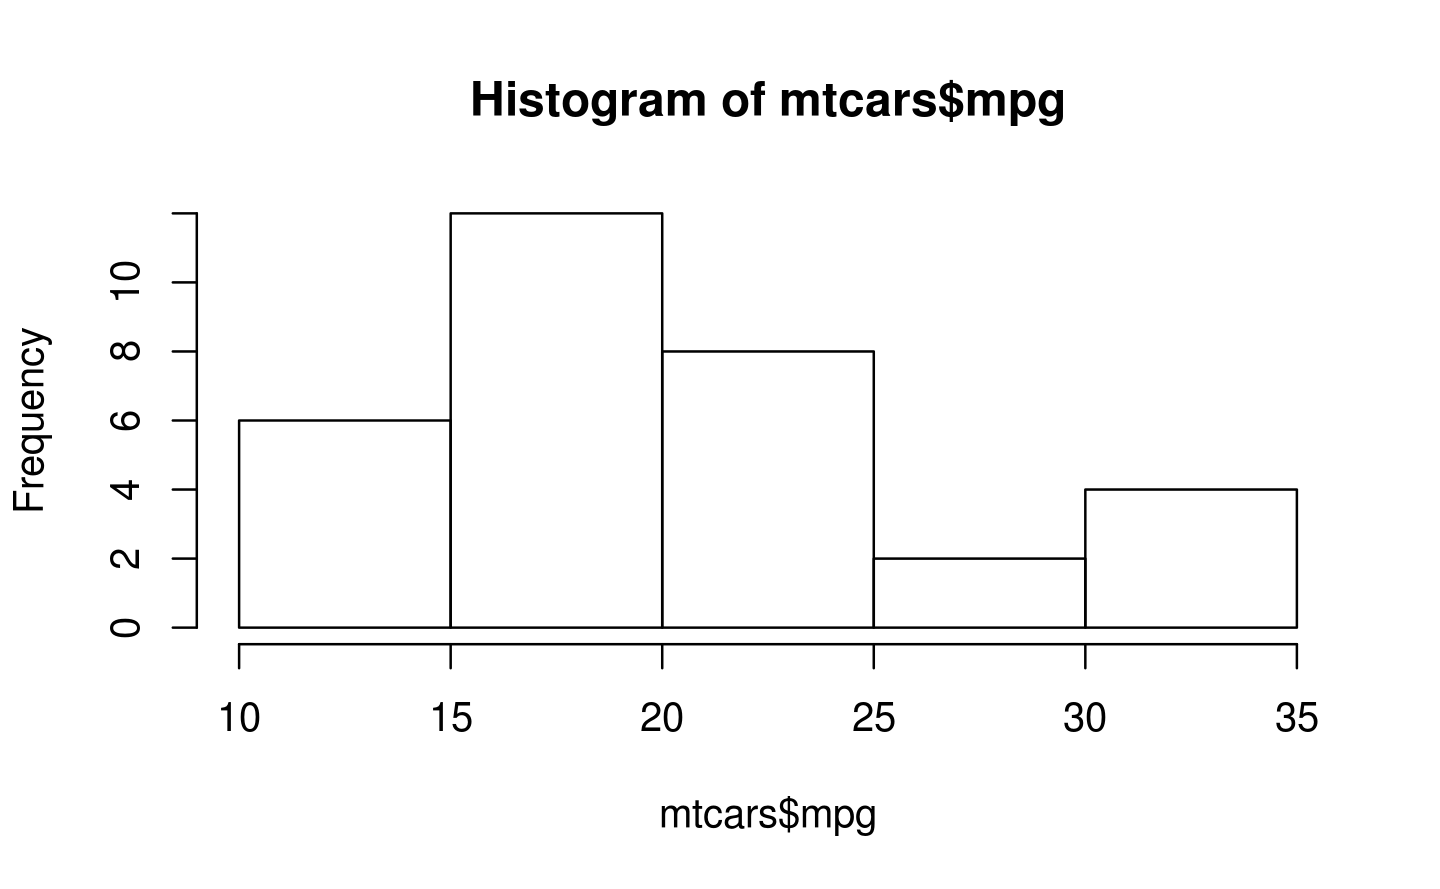
\includegraphics[width=0.7\linewidth]{rmi_copy_test_files/figure-latex/unnamed-chunk-417-1} \end{center}

\chapter{rbook 提要}\label{rbook-}

\section{index.Rmd}\label{index.rmd}

通常是一系列文章裡面的第一個文件。其他rmd文件的yml
頭部都可以統一放在這裡。

下面是一些選項,可以自行添加到上面:

\begin{Shaded}
\begin{Highlighting}[]
\FunctionTok{bibliography:}\AttributeTok{ }\KeywordTok{[}\NormalTok{book.bib}\KeywordTok{,}\NormalTok{ packages.bib}\KeywordTok{]}
\FunctionTok{biblio-style:}\AttributeTok{ apalike}
\FunctionTok{link-citations:}\AttributeTok{ yes}
\FunctionTok{github-repo:}\AttributeTok{ rstudio/bookdown-demo}
\end{Highlighting}
\end{Shaded}

bibliography 暫時沒有參考文件檔,所以我沒有放.

\hypertarget{section-1}{\section{}\label{section-1}}

\begin{itemize}
\tightlist
\item
  \href{https://rmarkdown.rstudio.com/r_notebook_format.html}{HTML
  Format} 來自\href{https://github.com/rstudio/rmarkdown}{rmarkdown from
  rstudio}
\item
  \href{http://conjugateprior.org/2012/12/r-markdown-to-other-document-formats/}{pandox}
\end{itemize}

\section{其他\_output.yml 範例}\label{_output.yml-}

簡單講,\_output.yml放的是輸出到哪裡?gitbook? pdf? 或者是簡單html格式。

::: sidebar \#\# \_output.yml 範例

\begin{Shaded}
\begin{Highlighting}[]
\FunctionTok{bookdown:}\AttributeTok{:gitbook:}
  \FunctionTok{css:}\AttributeTok{ style.css}
  \FunctionTok{config:}
    \FunctionTok{toc:}
      \FunctionTok{before:}\AttributeTok{ |}
\NormalTok{        <li><a href=}\StringTok{"./"}\NormalTok{>A Minimal Book Example</a></li>}
      \FunctionTok{after:}\AttributeTok{ |}
        \FunctionTok{<li><a href="https:}\AttributeTok{//github.com/rstudio/bookdown" target="blank">Published with bookdown</a></li>}
    \FunctionTok{edit:}\AttributeTok{ https://github.com/rstudio/bookdown-demo/edit/master/%s}
    \FunctionTok{download:}\AttributeTok{ }\KeywordTok{[}\StringTok{"pdf"}\KeywordTok{,} \StringTok{"epub"}\KeywordTok{]}

\CommentTok{# bookdown::pdf_book:}
\CommentTok{#   latex_engine: "xelatex"}
\CommentTok{#   keep_tex: true}
\CommentTok{#   includes:}
\CommentTok{#     in_header: header.tex}

 \FunctionTok{bookdown:}\AttributeTok{:pdf_book:}
   \FunctionTok{includes:}
     \FunctionTok{in_header:}\AttributeTok{ latex/preamble.tex}
     \FunctionTok{before_body:}\AttributeTok{ latex/before_body.tex}
     \FunctionTok{after_body:}\AttributeTok{ latex/after_body.tex}
   \FunctionTok{keep_tex:}\AttributeTok{ true}
   \FunctionTok{dev:}\AttributeTok{ }\StringTok{"cairo_pdf"}
   \FunctionTok{latex_engine:}\AttributeTok{ xelatex}
   \FunctionTok{citation_package:}\AttributeTok{ natbib}
   \FunctionTok{pandoc_args:}\AttributeTok{ }\KeywordTok{[}\StringTok{"--top-level-division=chapter"}\KeywordTok{,} \StringTok{"--lua-filter=latex/sidebar.lua"}\KeywordTok{]}
   \FunctionTok{template:}\AttributeTok{ }\DataTypeTok{null}
   \FunctionTok{quote_footer:}\AttributeTok{ }\DataTypeTok{null}
   \FunctionTok{toc_unnumbered:}\AttributeTok{ false}
   \FunctionTok{number_sections:}\AttributeTok{ true    }
\end{Highlighting}
\end{Shaded}

\begin{longtable}[]{@{}l@{}}
\caption{::}\tabularnewline
\toprule
``` yml\tabularnewline
\midrule
\endfirsthead
\toprule
``` yml\tabularnewline
\midrule
\endhead
output:\tabularnewline
html\_document:\tabularnewline
highlight: tango\tabularnewline
number\_sections: yes\tabularnewline
toc: yes\tabularnewline
\bottomrule
\end{longtable}

``\texttt{上面這段YML會被解譯到下面的R程式碼。\ 猜測:html\_document對應rmarkdown::html\_document\ \ \ 例如,\ number\_sections:\ yes\ 會被當成}html\_document()`的參數轉譯:

highlight: tango 對應到參數(沒有在下面)

\begin{Shaded}
\begin{Highlighting}[]
\NormalTok{rmarkdown}\OperatorTok{::}\KeywordTok{html_document}\NormalTok{( }\DataTypeTok{theme=} \StringTok{"lumen"}\NormalTok{,}
                               \DataTypeTok{template=}\NormalTok{ template,}
                               \DataTypeTok{css=}\NormalTok{ css,}
                               \DataTypeTok{toc=}\NormalTok{ toc,}
                               \DataTypeTok{toc_float=} \OtherTok{TRUE}\NormalTok{,}
                               \DataTypeTok{toc_depth=} \DecValTok{2}\NormalTok{,}
                               \DataTypeTok{number_sections=}\NormalTok{ number_sections,}
                               \DataTypeTok{df_print =} \StringTok{"paged"}\NormalTok{,}
                               \DataTypeTok{code_folding =}\NormalTok{ code_folding,}
                               \DataTypeTok{includes =} \KeywordTok{includes}\NormalTok{(}\DataTypeTok{before_body =}\NormalTok{ header)}
\NormalTok{                            )}
\ErrorTok{\}}
\end{Highlighting}
\end{Shaded}

\section{.travis.yml}\label{travis.yml}

\begin{quote}
\href{http://www.goring.org/resources/Adding_CI_To_RMarkdown.html}{rmarkdown
and travis}
\end{quote}

應該是用來指導怎麼建立專案的一個yml。 已知的部分有: directories :
可以指定子目錄,用來放暫存檔案(一些翻譯過程產生的中間黨),否則每個RMD都會產生一個組目錄。

\begin{Shaded}
\begin{Highlighting}[]
\FunctionTok{language:}\AttributeTok{ R}
\FunctionTok{sudo:}\AttributeTok{ false}
\FunctionTok{cache:}
  \FunctionTok{packages:}\AttributeTok{ true}
  \FunctionTok{directories:}
  \KeywordTok{-}\NormalTok{ _bookdown_files}
  \KeywordTok{-}\NormalTok{ $HOME/.npm}

\FunctionTok{pandoc_version:}\AttributeTok{ 2.1.1}
\end{Highlighting}
\end{Shaded}

\section{紀錄}

before\_chapter\_script: ``common.R'' 前面要有兩個空白

if(FALSE) \{ ' 兩個地方可以放, 1) 一個是在\_bookdown.yml中的最後一行:
before\_chapter\_script: ``common.R'' 2)一個是在每個RMD的第一個chunk執行
source(``common.R'')

' \}

\subsection{knitr hook}\label{knitr-hook}

\subsubsection{顏色}

設定警告訊息為紅色

\begin{Shaded}
\begin{Highlighting}[]
\NormalTok{knitr}\OperatorTok{::}\NormalTok{knit_hooks}\OperatorTok{$}\KeywordTok{set}\NormalTok{(}\DataTypeTok{error =} \ControlFlowTok{function}\NormalTok{(x, options) \{}
  \KeywordTok{paste0}\NormalTok{(}\StringTok{"<pre style=}\CharTok{\textbackslash{}"}\StringTok{color: red;}\CharTok{\textbackslash{}"}\StringTok{><code>"}\NormalTok{, x, }\StringTok{"</code></pre>"}\NormalTok{)}
\NormalTok{\})}
\end{Highlighting}
\end{Shaded}

其他範例

\begin{Shaded}
\begin{Highlighting}[]
\CommentTok{#Color Format}
\NormalTok{colFmt =}\StringTok{ }\ControlFlowTok{function}\NormalTok{(x,color)\{}
\NormalTok{  outputFormat =}\StringTok{ }\NormalTok{opts_knit}\OperatorTok{$}\KeywordTok{get}\NormalTok{(}\StringTok{"rmarkdown.pandoc.to"}\NormalTok{)}
  \ControlFlowTok{if}\NormalTok{(outputFormat }\OperatorTok{==}\StringTok{ 'latex'}\NormalTok{)}
    \KeywordTok{paste}\NormalTok{(}\StringTok{"}\CharTok{\textbackslash{}\textbackslash{}}\StringTok{textcolor\{"}\NormalTok{,color,}\StringTok{"\}\{"}\NormalTok{,x,}\StringTok{"\}"}\NormalTok{,}\DataTypeTok{sep=}\StringTok{""}\NormalTok{)}
  \ControlFlowTok{else} \ControlFlowTok{if}\NormalTok{(outputFormat }\OperatorTok{==}\StringTok{ 'html'}\NormalTok{)}
    \KeywordTok{paste}\NormalTok{(}\StringTok{"<font color='"}\NormalTok{,color,}\StringTok{"'>"}\NormalTok{,x,}\StringTok{"</font>"}\NormalTok{,}\DataTypeTok{sep=}\StringTok{""}\NormalTok{)}
  \ControlFlowTok{else}
\NormalTok{    x}
\NormalTok{\}}
\end{Highlighting}
\end{Shaded}

有關hook 的設定,參考
\href{https://yihui.name/knitr/hooks/\#output-hooks}{knitr hook}

\subsection{terminal output}\label{terminal-output}

問題:如果以要看檔案內容,而不想被無關的輸出符號干擾,例如{[}1{]},那麼如果再R
SCRIPT中可以使用 \texttt{system("cat\ 檔案名稱")} ,但是在R
Markdown中(如下)不會顯示出結果:

\begin{Shaded}
\begin{Highlighting}[]
\NormalTok{rst =}\StringTok{ }\KeywordTok{read.csv}\NormalTok{(}\StringTok{'resources/wh.csv'}\NormalTok{,}\DataTypeTok{comment.char=}\StringTok{"#"}\NormalTok{,}\DataTypeTok{na.string=}\StringTok{'.'}\NormalTok{)}
\KeywordTok{write.csv}\NormalTok{(rst, }\DataTypeTok{file =} \StringTok{"MyData.csv"}\NormalTok{,}\DataTypeTok{row.names=}\OtherTok{FALSE}\NormalTok{, }\DataTypeTok{na=}\StringTok{""}\NormalTok{)}
\KeywordTok{system}\NormalTok{(}\StringTok{"cat MyData.csv"}\NormalTok{)}
\end{Highlighting}
\end{Shaded}

You can use either

\{r, engine=`bash', comment=`'\} cat 'resources/hw.csv'

or

\begin{Shaded}
\begin{Highlighting}[]
\KeywordTok{cat}\NormalTok{(}\KeywordTok{readLines}\NormalTok{(}\StringTok{'resources/wh.csv'}\NormalTok{), }\DataTypeTok{sep =} \StringTok{'}\CharTok{\textbackslash{}n}\StringTok{'}\NormalTok{)}
\end{Highlighting}
\end{Shaded}

\section{python}\label{python}

First you need to set the knitr options.

\{r\} knitr::opts\_chunk\$set(engine.path = list(python =
`/anaconda/bin/python')) @@@ From that point on it just works.

\{python\} import this @@@ --\textgreater{}

\section{產生PDF 文件}\label{pdf-}

有關一些中文常常發生的錯誤:

\begin{itemize}
\tightlist
\item
  無法解決字型錯誤:Package fontspec Error: The font ``Inconsolata''
  cannot be found 改用其他字形
\end{itemize}

::: sidebar

\subsection{測試中文轉pdf}\label{pdf}

下列的檔案名稱為\texttt{x1.tx},測試的時候,可以利用\texttt{tinytex::xelatex(x1.tex)}
用來驗證是否中文可以轉pdf。

\begin{Shaded}
\begin{Highlighting}[]
\BuiltInTok{\textbackslash{}documentclass}\NormalTok{\{}\ExtensionTok{book}\NormalTok{\}}
\BuiltInTok{\textbackslash{}usepackage}\NormalTok{\{}\ExtensionTok{xeCJK}\NormalTok{\}}
\CommentTok{% \textbackslash{}setCJKmainfont\{Microsoft YaHei\}}
\FunctionTok{\textbackslash{}setCJKmainfont}\NormalTok{\{AR PL UMing TW\}}


\KeywordTok{\textbackslash{}begin}\NormalTok{\{}\ExtensionTok{document}\NormalTok{\}}
\NormalTok{早安,台灣}

\SpecialStringTok{$$a^2+b^2=c^2$$}

\NormalTok{Happy TeXing.}
\KeywordTok{\textbackslash{}end}\NormalTok{\{}\ExtensionTok{document}\NormalTok{\}}
\end{Highlighting}
\end{Shaded}

第一行\textbackslash{}documentclass\{book\}為什麼會在mybook專案中有衝突?
:::

\subsection{Overview}\label{overview}

\href{https://rmarkdown.rstudio.com/pdf_document_format}{參考}

\subsection{meta data 上的pdf 設定,常見版本}\label{meta-data-pdf-}

\begin{Shaded}
\begin{Highlighting}[]
\OtherTok{---}
\FunctionTok{title:}\AttributeTok{ }\StringTok{"Habits"}
\FunctionTok{author:}\AttributeTok{ lendjwjcen }
\FunctionTok{date:}\AttributeTok{ 3/1/2017}
\FunctionTok{output:}\AttributeTok{ pdf_document}
\OtherTok{---}
\end{Highlighting}
\end{Shaded}

\subsubsection{加入目錄}

\begin{Shaded}
\begin{Highlighting}[]
\OtherTok{---}
\FunctionTok{title:}\AttributeTok{ }\StringTok{"Habits"}
\FunctionTok{output:}
  \FunctionTok{pdf_document:}
    \FunctionTok{toc:}\AttributeTok{ true}
    \FunctionTok{toc_depth:}\AttributeTok{ 2}
\OtherTok{---}
\end{Highlighting}
\end{Shaded}

TOC深度預設是3。 yaml的註解符號是\texttt{\#} 。

如果要章節號碼,則利用\texttt{number\_sections\ option}:

\begin{Shaded}
\begin{Highlighting}[]
\OtherTok{---}
\FunctionTok{title:}\AttributeTok{ }\StringTok{"Habits"}
\FunctionTok{output:}
  \FunctionTok{pdf_document:}
    \FunctionTok{toc:}\AttributeTok{ true}
    \FunctionTok{number_sections:}\AttributeTok{ true}
\OtherTok{---}
\end{Highlighting}
\end{Shaded}

\subsubsection{圖形選項}

fig\_width 和 fig\_height 控制圖形的寬度和高度 (6 x 4.5 is used by
default)

fig\_crop 控制 pdfcrop utility (如果有)是否自動使用來修剪圖型(default).
如果我們的圖形設備是 postscript, 建議關掉這個選項。.

fig\_caption 控制是否有圖型標題(預設是否)

dev 控制用來描繪圖型的設備 (defaults to pdf)

例如:

\begin{Shaded}
\begin{Highlighting}[]
\OtherTok{---}
\FunctionTok{title:}\AttributeTok{ }\StringTok{"Habits"}
\FunctionTok{output:}
  \FunctionTok{pdf_document:}
    \FunctionTok{fig_width:}\AttributeTok{ 7}
    \FunctionTok{fig_height:}\AttributeTok{ 6}
    \FunctionTok{fig_caption:}\AttributeTok{ true}
\OtherTok{---}
\end{Highlighting}
\end{Shaded}

\subsubsection{Data Frame Printing}\label{data-frame-printing}

\texttt{df-print} 參數可以用來改進data frame的輸出,選項包括:

選項描述 default: 利用 print.data.frame 函數\\
kable 其實利用的是 knitr::kable 函數\\
tibble 則利用 tibble::print.tbl\_df 函數。.\\
例如:

\begin{Shaded}
\begin{Highlighting}[]
\OtherTok{---}
\FunctionTok{title:}\AttributeTok{ }\StringTok{"Habits"}
\FunctionTok{output:}
  \FunctionTok{pdf_document:}
    \FunctionTok{df_print:}\AttributeTok{ kable}
\OtherTok{---}
\end{Highlighting}
\end{Shaded}

\subsubsection{Syntax Highlighting}\label{syntax-highlighting}

打光型態有 ``default'', ``tango'', ``pygments'', ``kate'',
``monochrome'', ``espresso'', ``zenburn'', and ``haddock''
如果不要打光,則設定null:

例如:

\begin{Shaded}
\begin{Highlighting}[]
\OtherTok{---}
\FunctionTok{title:}\AttributeTok{ }\StringTok{"Habits"}
\FunctionTok{output:}
  \FunctionTok{pdf_document:}
    \FunctionTok{highlight:}\AttributeTok{ tango}
\OtherTok{---}
\end{Highlighting}
\end{Shaded}

\subsubsection{LaTeX Options}\label{latex-options}

有關LaTeX選項的設定位置並不是在\texttt{output:\ pdf\_document}的後續段落,而是在最頂層。
例如:

\begin{Shaded}
\begin{Highlighting}[]
\OtherTok{---}
\FunctionTok{title:}\AttributeTok{ }\StringTok{"Crop Analysis Q3 2013"}
\FunctionTok{output:}\AttributeTok{ pdf_document}
\FunctionTok{fontsize:}\AttributeTok{ 11pt}
\FunctionTok{geometry:}\AttributeTok{ margin=1in}
\OtherTok{---}
\end{Highlighting}
\end{Shaded}

\subsubsection{其他}

Available metadata variables include:

\begin{longtable}[]{@{}ll@{}}
\toprule
\begin{minipage}[b]{0.05\columnwidth}\raggedright\strut
Variable\strut
\end{minipage} & \begin{minipage}[b]{0.05\columnwidth}\raggedright\strut
Description\strut
\end{minipage}\tabularnewline
\midrule
\endhead
\begin{minipage}[t]{0.05\columnwidth}\raggedright\strut
papersize\strut
\end{minipage} & \begin{minipage}[t]{0.05\columnwidth}\raggedright\strut
paper size, e.g. \texttt{letter}, \texttt{A4}\strut
\end{minipage}\tabularnewline
\begin{minipage}[t]{0.05\columnwidth}\raggedright\strut
lang\strut
\end{minipage} & \begin{minipage}[t]{0.05\columnwidth}\raggedright\strut
Document language code\strut
\end{minipage}\tabularnewline
\begin{minipage}[t]{0.05\columnwidth}\raggedright\strut
fontsize\strut
\end{minipage} & \begin{minipage}[t]{0.05\columnwidth}\raggedright\strut
Font size (e.g.~10pt, 11pt, 12pt)\strut
\end{minipage}\tabularnewline
\begin{minipage}[t]{0.05\columnwidth}\raggedright\strut
documentclass\strut
\end{minipage} & \begin{minipage}[t]{0.05\columnwidth}\raggedright\strut
LaTeX document class (e.g.~article)\strut
\end{minipage}\tabularnewline
\begin{minipage}[t]{0.05\columnwidth}\raggedright\strut
classoption\strut
\end{minipage} & \begin{minipage}[t]{0.05\columnwidth}\raggedright\strut
Option for documentclass (e.g.~oneside); may be repeated\strut
\end{minipage}\tabularnewline
\begin{minipage}[t]{0.05\columnwidth}\raggedright\strut
geometry\strut
\end{minipage} & \begin{minipage}[t]{0.05\columnwidth}\raggedright\strut
Options for geometry class (e.g.~margin=1in); may be repeated\strut
\end{minipage}\tabularnewline
\begin{minipage}[t]{0.05\columnwidth}\raggedright\strut
linkcolor, urlcolor, citecolor\strut
\end{minipage} & \begin{minipage}[t]{0.05\columnwidth}\raggedright\strut
Color for internal, external, and citation links (red, green, magenta,
cyan, blue, black)\strut
\end{minipage}\tabularnewline
\begin{minipage}[t]{0.05\columnwidth}\raggedright\strut
thanks\strut
\end{minipage} & \begin{minipage}[t]{0.05\columnwidth}\raggedright\strut
specifies contents of acknowledgments footnote after document
title.\strut
\end{minipage}\tabularnewline
\bottomrule
\end{longtable}

更多控制可以在
\href{http://pandoc.org/MANUAL.html\#variables-for-latex}{here}.找到

\subsection{LaTeX Packages for
Citations}\label{latex-packages-for-citations}

citation的處理,預設是經由
\texttt{pandoc-citeproc}(不僅PDF文件,還有HTML),
但是對於PDF來講,最好還是使用 LaTeX 來處理例如 \texttt{natbib} or
\texttt{biblatex}。設定方法僅僅是設定 \texttt{citation\_package} 為
\texttt{natbib} 或 \texttt{biblatex}, 例如:

\begin{Shaded}
\begin{Highlighting}[]
\OtherTok{---}
\FunctionTok{output:}
  \FunctionTok{pdf_document:}
    \FunctionTok{citation_package:}\AttributeTok{ natbib}
\OtherTok{---}
\end{Highlighting}
\end{Shaded}

\section{中文}

建立中文PDF 需要安裝 TeX版本可以使用\texttt{tinytex}。

\begin{Shaded}
\begin{Highlighting}[]
\KeywordTok{install.packages}\NormalTok{(}\StringTok{'tinytex'}\NormalTok{)}
\NormalTok{tinytex}\OperatorTok{::}\KeywordTok{install_tinytex}\NormalTok{()}
\end{Highlighting}
\end{Shaded}

\section{Rstudio chinese}\label{rstudio-chinese}

\begin{Shaded}
\begin{Highlighting}[]
\BuiltInTok{cd}\NormalTok{ /usr/lib/rstudio/bin}
\FunctionTok{sudo}\NormalTok{ mkdir Qt}
\FunctionTok{sudo}\NormalTok{ mv libQt5* Qt}
\FunctionTok{sudo}\NormalTok{ mv qt.conf Qt}
\end{Highlighting}
\end{Shaded}

\subsubsection{拷貝Windows字型}\label{indows}

\begin{enumerate}
\def\labelenumi{\arabic{enumi}.}
\item
  建立Windows字型目錄WinFonts和Adobe字型目錄AdobeFonts。

\begin{Shaded}
\begin{Highlighting}[]
 \FunctionTok{sudo}\NormalTok{ mkdir /usr/share/fonts/WinFonts}
 \FunctionTok{sudo}\NormalTok{ mkdir /usr/share/fonts/AdobeFonts}
\end{Highlighting}
\end{Shaded}

  WinFonts位於\texttt{C:\textbackslash{}Windows\textbackslash{}fonts\textbackslash{}}文件夾下,只要ttf格式的中文字體;Adobe的字型則位於它的安裝目錄下,一個名叫font的文件夾內。
\item
  複製上述準備的字型到各自目錄。

\begin{Shaded}
\begin{Highlighting}[]
 \FunctionTok{sudo}\NormalTok{ cp /media/Ushe/WindowsFonts/* /usr/share/fonts/WinFonts}
 \FunctionTok{sudo}\NormalTok{ cp /media/Ushe/AdobeFonts/* /usr/share/fonts/AdobeFonts}
\end{Highlighting}
\end{Shaded}

  這裡需要注意:修改上面拷貝字型的許可權

\begin{Shaded}
\begin{Highlighting}[]
          \FunctionTok{sudo}\NormalTok{ chmod 644 /usr/share/fonts/WinFonts/*}

          \FunctionTok{sudo}\NormalTok{ chmod 644 /usr/share/fonts/AdobeFonts/*}
\end{Highlighting}
\end{Shaded}

  如果沒有這一步,會在編譯tex文件時出現下面類似的錯誤:

\begin{verbatim}
      SimSun at 17.28pt not loadable
\end{verbatim}
\item
  重新整理字型快取

\begin{Shaded}
\begin{Highlighting}[]
\FunctionTok{sudo}\NormalTok{  mkfontscale}
\FunctionTok{sudo}\NormalTok{  mkfontdir}
\FunctionTok{sudo}\NormalTok{  fc-cache -fsv}
\end{Highlighting}
\end{Shaded}

  \subsection{LaTeX Engine}\label{latex-engine}

  RStudio 預設使用 \texttt{pdflatex}. 我們可以使用
  \texttt{latex\_engine} 選項設定其他引擎例如, ``pdflatex'',
  ``xelatex'', and ``lualatex''. 而中文的引擎範例:

\begin{Shaded}
\begin{Highlighting}[]
\OtherTok{---}
\FunctionTok{title:}\AttributeTok{ }\StringTok{"Habits"}
\FunctionTok{output:}
  \FunctionTok{pdf_document:}
\FunctionTok{latex_engine:}\AttributeTok{ xelatex}
\OtherTok{---}
\end{Highlighting}
\end{Shaded}

  但是只有這樣還不夠,因為我們需要中文字型,這時可以利用\texttt{indclude}選項:\\
  \#\#\# Include
  要在文件本身(body)前面後面加上一些內容,可以利用\texttt{includes} 選項:
\end{enumerate}

\begin{Shaded}
\begin{Highlighting}[]
\OtherTok{---}
\FunctionTok{title:}\AttributeTok{ }\StringTok{"Habits"}
\FunctionTok{output:}
  \FunctionTok{pdf_document:}
    \FunctionTok{includes:}
      \FunctionTok{in_header:}\AttributeTok{ header.tex}
      \FunctionTok{before_body:}\AttributeTok{ doc_prefix.tex}
      \FunctionTok{after_body:}\AttributeTok{ doc_suffix.tex}
\OtherTok{---}
\end{Highlighting}
\end{Shaded}

::: sidebar 最後的中文設定可以是這樣

\begin{Shaded}
\begin{Highlighting}[]

\OtherTok{---}
\FunctionTok{title:}\AttributeTok{ }\StringTok{"Untitled"}
\FunctionTok{author:}\AttributeTok{ }\StringTok{"lin"}
\FunctionTok{date:}\AttributeTok{ }\StringTok{""}
\FunctionTok{output:}
  \FunctionTok{pdf_document:}\AttributeTok{ }
    \FunctionTok{latex_engine:}\AttributeTok{ xelatex    }
    \FunctionTok{includes:}
      \FunctionTok{in_header:}\AttributeTok{ header.tex    }
\end{Highlighting}
\end{Shaded}

\texttt{header.tex}的內容(\%是註解):

\begin{verbatim}
\usepackage{xeCJK}
% microsoft windows
% \setCJKmainfont{Microsoft YaHei}
\setCJKmainfont{NotoSansCJK}
% \setCJKmainfont{微軟正黑體}
%\setmainfont{Georgia} % 設定英文字型
%\setromanfont{Georgia} % 字型
%\setmonofont{Courier New}
\end{verbatim}

:::

好像沒用到 在ubuntu 中,移除Tex Live
\texttt{bash\ \ sudo\ apt-get\ purge\ texlive-*\ sudo\ apt-get\ autoremove\ sudo\ apt-get\ autoclean}
\#\#\# Custom Templates 也可以利用選項\texttt{template} 取代pandoc 模板
:

\begin{Shaded}
\begin{Highlighting}[]
\OtherTok{---}
\FunctionTok{title:}\AttributeTok{ }\StringTok{"Habits"}
\FunctionTok{output:}
  \FunctionTok{pdf_document:}
    \FunctionTok{template:}\AttributeTok{ quarterly_report.tex}
\OtherTok{---}
\end{Highlighting}
\end{Shaded}

參考 \href{http://pandoc.org/README.html\#templates}{pandoc templates}
上的說明。或者參考
\href{https://github.com/jgm/pandoc-templates/blob/master/default.latex}{default
LaTeX template} 中的範例。

\subsection{Pandoc Arguments}\label{pandoc-arguments}

如果在YAML中找不到相關於pandoc的選項,則可以直接利用
\texttt{pandoc\_args}. 例如:

\begin{Shaded}
\begin{Highlighting}[]
\OtherTok{---}
\FunctionTok{title:}\AttributeTok{ }\StringTok{"Habits"}
\FunctionTok{output:}
  \FunctionTok{pdf_document:}
    \FunctionTok{pandoc_args:}\AttributeTok{ }\KeywordTok{[}
      \StringTok{"--no-tex-ligatures"}
    \KeywordTok{]}
\OtherTok{---}
\end{Highlighting}
\end{Shaded}

\section{共用設定}

多個文件如果都有一樣的輸出格式,則可以利用檔案 \texttt{\_output.yaml}
例如:

**\_output.yaml**

\begin{Shaded}
\begin{Highlighting}[]
\FunctionTok{pdf_document:}
  \FunctionTok{toc:}\AttributeTok{ true}
  \FunctionTok{highlight:}\AttributeTok{ zenburn}
\end{Highlighting}
\end{Shaded}

做為文件中的YAML的比對,可以發現,只是把output:
的後面整個層級搬到\_output.yaml。

\begin{Shaded}
\begin{Highlighting}[]
\OtherTok{---}
\FunctionTok{title:}\AttributeTok{ }\StringTok{"Habits"}
\FunctionTok{output:}
  \FunctionTok{pdf_document:}
    \FunctionTok{includes:}
      \FunctionTok{in_header:}\AttributeTok{ header.tex}
      \FunctionTok{before_body:}\AttributeTok{ doc_prefix.tex}
      \FunctionTok{after_body:}\AttributeTok{ doc_suffix.tex}
\OtherTok{---}
\end{Highlighting}
\end{Shaded}

\section{討論}

\begin{itemize}
\tightlist
\item
  \href{https://github.com/lmmx/devnotes/wiki/Rmarkdown-custom-knit-hook-to-compile-a-multi-part-document}{hook}\\
  \href{https://rmarkdown.rstudio.com/articles_verbatim2.html}{Verbatim
  Chunks in R Markdow}\\
  *\href{https://github.com/rstudio/rmarkdown-book/blob/master/16-widgets.Rmd}{HTML
  widgets}\\
\item
  \href{https://rmarkdown.rstudio.com/r_notebook_format.html}{R Notebook
  HTML FOrmat}\\
\item
  \href{http://brooksandrew.github.io/simpleblog/articles/render-reports-directly-from-R-scripts/}{Render
  option}
  \href{https://selbydavid.com/2017/06/18/rmarkdown-alerts/}{hook
  example}\\
  *\href{https://gist.github.com/yihui/2629886}{more}\\
  \href{https://github.com/yihui/knitr-book}{dynamic book}
\end{itemize}

\subsection{inline code}\label{inline-code}

inline 讓內籤R程式碼不作用:方法是兩邊打上``。例如:

\begin{Shaded}
\begin{Highlighting}[]
\KeywordTok{inline}\NormalTok{(}\StringTok{"dd"}\NormalTok{)}
\OperatorTok{==}\ErrorTok{=>}\StringTok{  ``} \StringTok{`}\DataTypeTok{r dd}\StringTok{`} \StringTok{``}
\end{Highlighting}
\end{Shaded}

\begin{Shaded}
\begin{Highlighting}[]
\KeywordTok{cat}\NormalTok{(readr}\OperatorTok{::}\KeywordTok{read_file}\NormalTok{(}\StringTok{"rmd_topic_1.Rmd"}\NormalTok{))}
\end{Highlighting}
\end{Shaded}

\begin{Shaded}
\begin{Highlighting}[]
\NormalTok{rst =}\StringTok{ }\KeywordTok{read.csv}\NormalTok{(}\StringTok{'resources/wh.csv'}\NormalTok{,}\DataTypeTok{comment.char=}\StringTok{"#"}\NormalTok{,}\DataTypeTok{na.string=}\StringTok{'.'}\NormalTok{)}
\KeywordTok{write.csv}\NormalTok{(rst, }\DataTypeTok{file =} \StringTok{"MyData.csv"}\NormalTok{,}\DataTypeTok{row.names=}\OtherTok{FALSE}\NormalTok{, }\DataTypeTok{quote=}\NormalTok{F)}
\CommentTok{# system("cat myData.csv") # 這個不行}
\KeywordTok{cat}\NormalTok{(}\KeywordTok{readLines}\NormalTok{(}\StringTok{'MyData.csv'}\NormalTok{), }\DataTypeTok{sep =} \StringTok{'}\CharTok{\textbackslash{}n}\StringTok{'}\NormalTok{)}
\end{Highlighting}
\end{Shaded}

\begin{Shaded}
\begin{Highlighting}[]
\KeywordTok{cat}\NormalTok{(readr}\OperatorTok{::}\KeywordTok{read_file}\NormalTok{(}\StringTok{"MyData.csv"}\NormalTok{))}
\end{Highlighting}
\end{Shaded}

mtcas 中的資料筆數有 32

\chapter{gitbook introduction}\label{gitbook-introduction}

3個地方需要注意: \_output.yml \_bookdown.yml index.rmd

\section{\_output.yml:}\label{output.yml}

\begin{Shaded}
\begin{Highlighting}[]
\FunctionTok{bookdown:}\AttributeTok{:gitbook:}
  \FunctionTok{css:}\AttributeTok{ style.css}
  \FunctionTok{split_by:}\AttributeTok{ chapter}
  \FunctionTok{config:}
    \FunctionTok{toc:}
      \FunctionTok{collapse:}\AttributeTok{ subsection}
      \FunctionTok{before:}\AttributeTok{ |}
\NormalTok{        <li><a href=}\StringTok{"./"}\NormalTok{>A Minimal Bookdown Book</a></li>}
      \FunctionTok{after:}\AttributeTok{ |}
        \FunctionTok{<li><a href="https:}\AttributeTok{//github.com/rstudio/bookdown" target="blank">Published with bookdown</a></li>}
\FunctionTok{bookdown:}\AttributeTok{:pdf_book:}
  \FunctionTok{includes:}
    \FunctionTok{in_header:}\AttributeTok{ preamble.tex}
  \FunctionTok{latex_engine:}\AttributeTok{ xelatex}
  \FunctionTok{citation_package:}\AttributeTok{ natbib}
\FunctionTok{bookdown:}\AttributeTok{:epub_book:}
  \FunctionTok{stylesheet:}\AttributeTok{ style.css}
  
\end{Highlighting}
\end{Shaded}

上面要修改的部分只有書名(title of book)

\section{\_bookdown.yml:}\label{bookdown.yml}

\begin{Shaded}
\begin{Highlighting}[]

\FunctionTok{book_filename:}\AttributeTok{ }\StringTok{"bookdown-xx"}
\FunctionTok{chapter_name:}\AttributeTok{ }\StringTok{"Chapter "}
\FunctionTok{repo:}\AttributeTok{ https://github.com/seankross/bookdown-start}
\FunctionTok{output_dir:}\AttributeTok{ docs}
\FunctionTok{rmd_files:}\AttributeTok{ }\KeywordTok{[}\StringTok{"index.Rmd"}\KeywordTok{,} \StringTok{"01-Introduction.Rmd"}\KeywordTok{,} \StringTok{"02-Diving-In.Rmd"}\KeywordTok{]}
\FunctionTok{clean:}\AttributeTok{ }\KeywordTok{[}\NormalTok{packages.bib}\KeywordTok{,}\NormalTok{ bookdown.bbl}\KeywordTok{]}
\FunctionTok{new_session:}\AttributeTok{ yes}
\end{Highlighting}
\end{Shaded}

\begin{itemize}
\tightlist
\item
  欄位 book\_filename :書名(PDF
  或EPUB)例如本例的書名為bookdown\_xx.pdf。\\
\item
  欄位 chapter\_name:每個章節的前綴,例如 01-Introduction.Rmd 第一個H1
  標籤為 \# Introduction ,會變成 ``Chapter 1 Introduction''。\\
\item
  欄位 repo field just designates a GitHub repository associated with
  this book but this is not a required field.\\
\item
  欄位 output\_dir:
  HTML檔案的輸出位置。同時也是pdf檔案的輸出位置。如果沒有設定這個欄位,那麼預設輸出位置是
  \_book/ 。\\
\item
  欄位
  rmd\_files:這是選擇性的,如果沒有設定,那麼專案子目錄下的所有RMD都會被rendered。\\
\item
  欄位 new\_session: 這也是選擇性的。如果是 new\_session: yes
  那麼每個RMD都在新的R連結(session)描繪(rendered),否則在同一個session.
\end{itemize}

::: sidebar \#\# new\_session 注意事項 但是我注意到,new\_session
設定為yes的時候,md檔案會被留下,而設定為no的時候,則不會。

同時,在new\_session=no的時候,可以指定子目錄中的RMD檔案。

例如

\begin{Shaded}
\begin{Highlighting}[]
\FunctionTok{language:}
  \FunctionTok{ui:}
    \FunctionTok{chapter_name:}\AttributeTok{ }\StringTok{"Chapter "}
\FunctionTok{new_session:}\AttributeTok{ no}
\FunctionTok{after_chapter_script:}\AttributeTok{ clear_vars_and_pkgs.R}
\FunctionTok{rmd_files:}
  \KeywordTok{-} \StringTok{"index.Rmd"}
  \KeywordTok{-} \StringTok{"my_sub_dir/chapter1.Rmd"}
  \KeywordTok{-} \StringTok{"my_sub_dir/chapter2.Rmd"}
\end{Highlighting}
\end{Shaded}

注意: new\_session=yes
的時候,會產生md檔案,如果上傳到Github會被jekyll解讀
要避免這個情況發生,推測兩個解法 1. (OK) 在docs中放入.nojkeyll
這個檔案(在bash中執行指令 touch .nojkeyll)\\
1. (不確定)在\_bookdown.yml
的欄位after\_chapter\_script:中指定執行指令殺掉所有md檔案\\
::: \#\# index.rmd 另外一個相關設定的地方是index.rmd
。這個檔案用來設定書的cover, 和前幾頁。因此Preface
和簡介可以放在這個檔案。這個檔案的前幾行通常是有關yaml的一些設定,例如

\begin{Shaded}
\begin{Highlighting}[]
\OtherTok{---}
\FunctionTok{title:}\AttributeTok{ }\StringTok{"XXX title"}
\FunctionTok{author:}\AttributeTok{ }\StringTok{"len jwj cen"}
\FunctionTok{date:}\AttributeTok{ }\StringTok{"2018-1-1"}
\FunctionTok{site:}\AttributeTok{ bookdown::bookdown_site}
\FunctionTok{documentclass:}\AttributeTok{ book}
\CommentTok{#bibliography: [book.bib]}
\CommentTok{#biblio-style: apalike}
\FunctionTok{link-citations:}\AttributeTok{ yes}
\FunctionTok{github-repo:}\AttributeTok{ seankross/bookdown-start}
\FunctionTok{url:}\AttributeTok{ }\StringTok{'http\textbackslash{}://seankross.com/bookdown-start/'}
\FunctionTok{description:}\AttributeTok{ }\StringTok{"gitbook's simple setup"}
\OtherTok{---}
\end{Highlighting}
\end{Shaded}

應該更改的有 title, author, date, github-repo, url, and description
欄位。 其他設定有 cover-image:圖檔位置。

::: sidebar site: bookdown::bookdown\_site 有這行就不用設定\_site.yml。

::: \#\# 執行

bookdown::render\_book(``index.Rmd'')

\section{加入:Travis}\label{travis}

使用 Travis 產生書一需要3個檔案,這三個黨要放在github repo的根目錄:
3個檔案的前2個,可以直接從這裡複製: \#\#\# .Rbuildignore

\^{}.*.Rproj\$ \textsuperscript{.Rproj.user\$ }.travis.yml\$

\subsection{.travis.yml:}\label{travis.yml-1}

\begin{Shaded}
\begin{Highlighting}[]
\FunctionTok{language:}\AttributeTok{ r}
\FunctionTok{cache:}\AttributeTok{ packages}

\FunctionTok{script:}
  \KeywordTok{-} \FunctionTok{Rscript -e 'bookdown:}\AttributeTok{:render_book("index.rmd")'}
\end{Highlighting}
\end{Shaded}

\subsection{DESCRIPTION}\label{description}

要讓travis誤認為package 所以,只是放著,內容不管

\begin{verbatim}
Package: placeholder
Title: Does not matter.
Version: 0.0.1
Imports: bookdown
Remotes: rstudio/bookdown
\end{verbatim}


\end{document}
